% The Not So Short Introduction to LaTeX
%
% Copyright (C) 1995--2022 Tobias Oetiker, Marcin Serwin, Hubert Partl,
% Irene Hyna, Elisabeth Schlegl and Contributors.
%
% This document is free software: you can redistribute it and/or modify it
% under the terms of the GNU General Public License as published by the Free
% Software Foundation, either version 3 of the License, or (at your option) any
% later version.
%
% This document is distributed in the hope that it will be useful, but WITHOUT
% ANY WARRANTY; without even the implied warranty of MERCHANTABILITY or FITNESS
% FOR A PARTICULAR PURPOSE.  See the GNU General Public License for more
% details.
%
% You should have received a copy of the GNU General Public License along with
% this document.  If not, see <https://www.gnu.org/licenses/>.
% !TEX root = ./lshort.tex

%%%%%%%%%%%%%%%%%%%%%%%%%%%%%%%%%%%%%%%%%%%%%%%%%%%%%%%%%%%%%%%%%
% Contents: Main Input File of the LaTeX2e Introduction
% $Id$
%%%%%%%%%%%%%%%%%%%%%%%%%%%%%%%%%%%%%%%%%%%%%%%%%%%%%%%%%%%%%%%%%
% lshort.tex - The not so short introduction to LaTeX
%                                                      by Tobias Oetiker
%                                                     oetiker@ee.ethz.ch
%
%                           based on LKURTZ.TEX Uni Graz & TU Wien, 1987
%-----------------------------------------------------------------------
%
% To compile lshort, you need TeX 3.x, LaTeX and makeindex
%
% The sources files of the Intro are:
%      lshort.tex (this file),
%      title.tex, contrib.tex, biblio.tex
%      things.tex, typeset.tex, math.tex, lssym.tex, spec.tex,
%      lshort.sty, fancyheadings.sty
%
% Further the  verbatim.sty and the layout.sty
% from the LaTeX Tools distribution is
% required.
%
%
% To print the AMS symbols you need the AMS fonts and the packages
% amsfonts, eufrak and eucal from (AMS LaTeX 1.2)
%
% ---------------------------------------------------------------------
\begin{document}
%%%%%%%%%%%%%%%%%%%%%%%%%%%%%%%%%%%%%%%%%%%%%%%%%%%%%%%%%%%%%%%%%
% Contents: The title page
% $Id$
%%%%%%%%%%%%%%%%%%%%%%%%%%%%%%%%%%%%%%%%%%%%%%%%%%%%%%%%%%%%%%%%%

\ifpdf
  \pdfbookmark{Title Page}{title}
\fi
\newlength{\centeroffset}
\setlength{\centeroffset}{-0.5\oddsidemargin}
\addtolength{\centeroffset}{0.5\evensidemargin}
%\addtolength{\textwidth}{-\centeroffset}
\thispagestyle{empty}
\vspace*{\stretch{1}}
\noindent\hspace*{\centeroffset}\makebox[0pt][l]{\begin{minipage}{\textwidth}
\flushright
{\Huge\bfseries The Not So Short\\ 
Introduction to \LaTeXe

}
\noindent\rule[-1ex]{\textwidth}{5pt}\\[2.5ex]
\hfill\emph{\Large Or \LaTeXe{} in \pageref{LastPage} minutes}
\end{minipage}}

\vspace{\stretch{1}}
\noindent\hspace*{\centeroffset}\makebox[0pt][l]{\begin{minipage}{\textwidth}
\flushright
{\bfseries 
by Tobias Oetiker\\[1.5ex]
Hubert Partl, Irene Hyna and  Elisabeth Schlegl\\[3ex]} 
Version~5.00, December 14, 2010
\end{minipage}}

%\addtolength{\textwidth}{\centeroffset}
\vspace{\stretch{2}}


\pagebreak
\begin{small} 
  Copyright \copyright 1995-2010 Tobias Oetiker and Contributors.  All rights reserved.
 
  This document is free; you can redistribute it and/or modify it
  under the terms of the GNU General Public License as published by
  the Free Software Foundation; either version 2 of the License, or
  (at your option) any later version.
  
  This document is distributed in the hope that it will be useful, but
  \emph{without any warranty}; without even the implied warranty of
  \emph{merchantability} or \emph{fittness for a particular purpose}\@.  See the GNU
  General Public License for more details.
  
  You should have received a copy of the GNU General Public License
  along with this document; if not, write to the Free Software
  Foundation, Inc., 675 Mass Ave, Cambridge, MA 02139, USA.

\end{small}


\endinput

%

% Local Variables:
% TeX-master: "lshort2e"
% mode: latex
% mode: flyspell
% End:

% The Not So Short Introduction to LaTeX
%
% Copyright (C) 1995--2022 Tobias Oetiker, Marcin Serwin, Hubert Partl,
% Irene Hyna, Elisabeth Schlegl and Contributors.
%
% This document is free software: you can redistribute it and/or modify it
% under the terms of the GNU General Public License as published by the Free
% Software Foundation, either version 3 of the License, or (at your option) any
% later version.
%
% This document is distributed in the hope that it will be useful, but WITHOUT
% ANY WARRANTY; without even the implied warranty of MERCHANTABILITY or FITNESS
% FOR A PARTICULAR PURPOSE.  See the GNU General Public License for more
% details.
%
% You should have received a copy of the GNU General Public License along with
% this document.  If not, see <https://www.gnu.org/licenses/>.

% !TEX root = ./lshort.tex
%%%%%%%%%%%%%%%%%%%%%%%%%%%%%%%%%%%%%%%%%%%%%%%%%%%%%%%%%%%%%%%%%
% Contents: Who contributed to this Document
% $Id$
%%%%%%%%%%%%%%%%%%%%%%%%%%%%%%%%%%%%%%%%%%%%%%%%%%%%%%%%%%%%%%%%%
\thispagestyle{empty}
\begin{small}
  \noindent Copyright \copyright{} 1995--2022 Tobias~Oetiker, Marcin~Serwin,
  Hubert~Partl, Irene~Hyna, Elisabeth~Schlegl and Contributors.

  This document is free software: you can redistribute it and/or modify it under
  the terms of the GNU General Public License as published by the Free Software
  Foundation, either version 3 of the License, or (at your option) any later
  version.

  This document is distributed in the hope that it will be useful, but
  \emph{without any warranty}; without even the implied warranty of
  \emph{merchantability} or \emph{fitness for a particular purpose}.  See
  the GNU General Public License for more details.

  You should have received a copy of the GNU General Public License along with
  this document.  If not, see \url{https://www.gnu.org/licenses/}.
  \vspace{-5pt}
  \begin{flushright}
    \href{https://www.gnu.org/licenses/gpl-3.0.html}{%
      \includegraphics[width=2cm]{images/gpl3.pdf}}\hspace*{10pt}
  \end{flushright}

  \bigskip\noindent The illustration on the first page was created for this booklet by Roman Schmid
  (\href{https://github.com/bummzack}{@bummzack} on GitHub). It is dedicated to the
  public domain via CC0 1.0 Universal
  Public Domain Dedication. This means that you can use it freely in your own
  work without any licensing issues. See
  \url{https://creativecommons.org/publicdomain/zero/1.0/} for more details.
  \vspace{-15pt}
  \begin{flushright}
    \href{https://creativecommons.org/publicdomain/zero/1.0/}{%
      \includegraphics[width=2cm]{images/cc-zero.pdf}}\hspace*{10pt}
  \end{flushright}

  \bigskip\noindent
  Additionally, the code examples (text written using \texttt{monospace font}
  in this document) are dedicated to the public domain via CC0 1.0 Universal
  Public Domain Dedication. This means that you can use them freely in your own
  work without any licensing issues. See
  \url{https://creativecommons.org/publicdomain/zero/1.0/} for more details.
  \vspace{-15pt}
  \begin{flushright}
    \href{https://creativecommons.org/publicdomain/zero/1.0/}{%
      \includegraphics[width=2cm]{images/cc-zero.pdf}}\hspace*{10pt}
  \end{flushright}

  \vspace{\stretch{1}}
  \noindent The full text of the GNU General Public License can be found in
  \autoref{gplfull} on \autopageref{gplfull}.
\end{small}
\cleardoublepage

\frontmatter
%%%%%%%%%%%%%%%%%%%%%%%%%%%%%%%%%%%%%%%%%%%%%%%%%%%%%%%%%%%%%%%%%
% Contents: Who contributed to this Document
% $Id$
%%%%%%%%%%%%%%%%%%%%%%%%%%%%%%%%%%%%%%%%%%%%%%%%%%%%%%%%%%%%%%%%%
\chapter{Thank you!}
\noindent Much of the material used in this introduction comes from an
Austrian introduction to \LaTeX\ 2.09 written in German by:
\begin{verse}
\contrib{Hubert Partl}{partl@mail.boku.ac.at}%
{Zentraler Informatikdienst der Universit\"at f\"ur Bodenkultur Wien}
\contrib{Irene Hyna}{Irene.Hyna@bmwf.ac.at}%
   {Bundesministerium f\"ur Wissenschaft und Forschung Wien}
\contrib{Elisabeth Schlegl}{no email}%
   {in Graz}
\end{verse}

If you are interested in the German document, you can find a version
updated for \LaTeXe{} by J\"org Knappen at\\
\CTAN|info/lshort/german|

\newpage \noindent The
following individuals helped with corrections, suggestions and
material to improve this paper. They put in a big effort to help me
get this document into its present shape. I would like to
sincerely thank all of them. Naturally, all the mistakes you'll find
in this book are mine. If you ever find a word that is spelled
correctly, it must have been one of the people below dropping me a
line.

{ \flushleft\small
Eric~Abrahamsen,        %eric@ericabrahamsen.net
Rosemary~Bailey,        %r.a.bailey@qmw.ac.uk 0.2
Marc~Bevand,            % <bevand_m@epita.fr>
Friedemann~Brauer,      %fbrauer@is.dal.ca 3.4
Barbara~Beeton,         %bnb@ams.org
Salvatore~Bonaccorso,   % bonaccos@ee.ethz.ch
Jan~Busa,               % <busaj@ccsun.tuke.sk>
Markus~Br\"uhwiler,     % <m.br@switzerland.org>
Pietro~Braione,         % <braione@elet.polimi.it>
David~Carlisle,         %GONE carlisle@cs.man.ac.uk 1.0
Jos\'e~Carlos~Santos,   % <jcsantos@fc.up.pt>
Neil~Carter,            % N.Carter@Swansea.ac.uk
Mike~Chapman,           %chapman@eeh.ee.ethz.ch 3.16
Pierre~Chardaire,       % <pc@sys.uea.ac.uk
Christopher~Chin,       %chris.chin@rmit.edu.au 3.1
Carl~Cerecke,           %cdc@cosc.canterbury.ac.nz>
Chris~McCormack,        %GONE chrismc@eecs.umich.edu 0.1
Wim~van~Dam,            %GONE wimvdam@cs.kun.nl 2.2
Jan~Dittberner,         %jan@jan-dittberner.de 3.15
Michael~John~Downes,    %<mjd@ams.org> 14 Oct 1999
Matthias~Dreier,        %dreier@ostium.ch
David~Dureisseix,       %dureisse@lmt.ens-cachan.fr 1.1
Eilinger~August,        % <eaugust@student.ethz.ch>
Elliot,                 %GONE enh-a@minster.york.ac.uk 1.1
Hans~Ehrbar,            %ehrbar@econ.utah.edu
Daniel~Flipo,           %Daniel.Flipo@univ-lille1.fr
David~Frey,             %david@eos.lugs.ch 2.2
Hans~Fugal,             %hans@fugal.net
Robin~Fairbairns,       %Robin.Fairbairns@cl.cam.ac.uk 0.2 1.0
J\"org~Fischer,        %j.fischer@xpoint.at 3.16
Erik~Frisk,             %frisk@isy.liu.se 3.4
Mic~Milic~Frederickx,   % <mic.milic@web.de>
Frank,                  %frank@freezone.co.uk 11 Feb 2000
Kasper~B.~Graversen,    % <kbg@dkik.dk>
Arlo~Griffiths,         % <A.Griffiths@let.leidenuniv.nl>
Alexandre~Guimond,      %guimond@IRO.UMontreal.CA 0.9
Andy~Goth,              % <unununium@openverse.com>
Cyril~Goutte,           %goutte@ei.dtu.dk 2.1 2.2
Greg~Gamble,            %gregg@maths.uwa.edu.au 2.2
Frank~Fischli,          % <fischlifaenger@gmx.ch>
Morten~H�gholm,		% morten.hoegholm@latex-project.org
Neil~Hammond,           %nfh@dmu.ac.uk 0.3
Rasmus~Borup~Hansen,    %GONE rbhfamos@math.ku.dk 0.2 0.9 0.91 0.92 1.9.9
Joseph~Hilferty,        % <hilferty@fil.ub.es>
Bj\"orn Hvittfeldt,     %bjorn@hvittfeldt.com 3.13
Martien~Hulsen,         %M.A.Hulsen@WbMt.TUDelft.NL 1.0 1.1
Werner~Icking,          %<Werner.Icking@gmd.de> 3.1
Jakob,                  %diness@get2net.dk
Eric~Jacoboni,          %GONE jacoboni@enseeiht.fr 0.1 0.9
Alan~Jeffrey,           %alanje@cogs.sussex.ac.uk 0.2
Byron~Jones,            %bj@dmu.ac.uk 1.1
David~Jones,            %GONE djones@CA.McMaster.dcss.insight 1.1
Nils~Kanning,           % <nils@kanning.de>
Tobias~Krewer,          %tobias.krewer@googlemail.com
Johannes-Maria~Kaltenbach, %<kaltenbach@zeiss.de> 3.01
Michael~Koundouros,     % <mkoundouros@hotmail.com>
Andrzej~Kawalec,        %GONE akawalec@prz.rzeszow.pl 1.9.9
Sander~de~Kievit,       %Skievit@ucu.uu.nl
Alain~Kessi,            %ALAIN_KESSI@HOTMAIL.COM 2.2
Christian~Kern,         %ck@unixen.hrz.uni-oldenburg.de 2.1
Tobias~Klauser,		%tklauser@access.unizh.ch 4.17
J\"org~Knappen,         %knappen@vkpmzd.kph.uni-mainz.de 0.1
Kjetil~Kjernsmo,        %<kjetil.kjernsmo@astro.uio.no> 3.2
Maik~Lehradt,           %greek@uni-paderborn.de 0.1
R\'emi~Letot,           % <r_letot@yahoo.com>
Flori~Lambrechts,       % <f.lambrechts@softhome.net>
Axel~Liljencrantz,	% <Axel.Liljencrantz@byv.kth.se>
Johan~Lundberg,         %p99jlu@physto.se
Alexander~Mai,          %Alexander.Mai@physik.tu-darmstadt.de 3.8
Hendrik~Maryns,         %hendrik.maryns@ugent.be
Martin~Maechler,        %<maechler@stat.math.ethz.ch> 2.2
Aleksandar~S~Milosevic, % <aleksandar.milosevic@yale.edu>
Henrik~Mitsch,          % <Henrik.Mitsch@gmx.at>
Claus~Malten,           %GONE <ASI138%BITNET.DJUKFA11@BITNET.CEARN> 1.1
Kevin~Van~Maren,        % <vanmaren@fast.cs.utah.edu>  24 Nov 1999
Stefan~M.~Moser,        % stefan.moser@ieee.org 
Richard~Nagy,           % r.nagy@nameshield.net
Philipp~Nagele,         % Philipp.Nagele@t-systems.com
Lenimar~Nunes~de~Andrade, % <lenimar@mat.ufpb.br> Fri, 12 Nov 1999
I.~J.~Vera~ Mar\'un,    % I.J.Veramarun@ewi.utwente.nl
Manuel~Oetiker,         % manuel@oetiker.ch
Urs~Oswald,             % osurs@bluewin.ch
Lan~Thuy~Pham,          %<lan.thuy.pham@gmail.com>
Martin~Pfister,		% m@rtinpfister.ch
Demerson~Andre~Polli,   % polli@linux.ime.usp.br
Nikos~Pothitos,		% <n.pothitos@di.uoa.gr>
Maksym~Polyakov         % <polyama@myrealbox.com>
Hubert~Partl,           %partl@mail.boku.ac.at 0.2 1.1
John~Refling,           %refling@sierra.lbl.gov 0.1 0.9
Mike~Ressler,           %ressler@cougar.jpl.nasa.gov 0.1 0.2 0.9 1.0 1.9.9
Brian~Ripley,           %ripley@stats.ox.ac.uk 2.1
Young~U.~Ryu,           %ryoung@utdallas.edu 2.1
Bernd~Rosenlecher,      %9rosenle@informatik.uni-hamburg.de 10 Feb 2000
Kurt~Rosenfeld,		%kurt@isis.poly.edu
Chris~Rowley,           %C.A.Rowley@open.ac.uk 0.91
Risto~Saarelma,         %risto.saarelma@cs.helsinki.fi
Hanspeter~Schmid,       %schmid@isi.ee.ethz.ch
Craig~Schlenter,        %cschle@lucy.ee.und.ac.za 0.1 0.2 0.9
Gilles~Schintgen,       %gschintgen@internet.lu
Baron~Schwartz,         % <bps7j@cs.virginia.edu>      
Christopher~Sawtell,    %<csawtell@xtra.co.nz> 1 Sep 1999
Miles~Spielberg,        %zeibach@hotmail.com
Matthieu~Stigler,       % table row height
Geoffrey~Swindale,      % <geofftswin@ntlworld.com>
Laszlo~Szathmary,       % <szathml@delfin.klte.hu>
Boris~Tobotras,         % <tobotras@jet.msk.su>
Josef~Tkadlec,          %tkadlec@math.feld.cvut.cz 2.0 2.2
Scott~Veirs,            %scottv@ocean.washington.edu
Didier~Verna,           %verna@inf.enst.fr 2.2
Fabian~Wernli,          %wernli@iap.fr 3.2
Carl-Gustav~Werner,     % <Carl-Gustav.Werner@math.lu.se> 11 Oct 1999,3.16
David~Woodhouse,        % <dwmw2@infradead.org> 3.16
Chris~York,             % <c.s.york@Cummins.com>  21 Nov 1999
Fritz~Zaucker,          %zaucker@ee.ethz.ch 3.0
Rick~Zaccone,           %zaccone@bucknell.edu 2.2
and Mikhail~Zotov.      %zotov@eas.npi.msu.su 3.1

}

\vspace*{\stretch{1}}



\pagebreak
\endinput
%

% Local Variables:
% TeX-master: "lshort2e"
% mode: latex
% mode: flyspell
% End:

%%%%%%%%%%%%%%%%%%%%%%%%%%%%%%%%%%%%%%%%%%%%%%%%%%%%%%%%%%%%%%%%%
% Contents: Who contributed to this Document
% $Id$
%%%%%%%%%%%%%%%%%%%%%%%%%%%%%%%%%%%%%%%%%%%%%%%%%%%%%%%%%%%%%%%%%

% Because this introduction is the reader's first impression, I have
% edited very heavily to try to clarify and economize the language.
% I hope you do not mind! I always try to ask "is this word needed?"
% in my own writing but I don't want to impose my style on you... 
% but here I think it may be more important than the rest of the book.
% --baron

\chapter{Preface}

\LaTeX{} \cite{manual} is a typesetting system that is very 
suitable for producing scientific and mathematical documents of high
typographical quality. It is also suitable for producing all
sorts of other documents, from simple letters to complete books.
\LaTeX{} uses \TeX{} \cite{texbook} as its formatting engine.

This short introduction describes \LaTeXe{} and should be sufficient
for most applications of \LaTeX. Refer to~\cite{manual,companion} for
a complete description of the \LaTeX{} system.

\bigskip
\noindent This introduction is split into 6 chapters:
\begin{description}
\item[Chapter 1] tells you about the basic structure of \LaTeXe{}
  documents. You will also learn a bit about the history of \LaTeX{}.
  After reading this chapter, you should have a rough understanding how
  \LaTeX{} works.
\item[Chapter 2] goes into the details of typesetting your
  documents. It explains most of the essential \LaTeX{} commands and
  environments. After reading this chapter, you will be able to write
  your first documents. 
\item[Chapter 3] explains how to typeset formulae with \LaTeX. Many
  examples demonstrate how to use one of \LaTeX{}'s
  main strengths. At the end of the chapter are tables listing
  all mathematical symbols available in \LaTeX{}.
\item[Chapter 4] explains indexes,  bibliography generation and
  inclusion of EPS graphics. It introduces creation of PDF documents with pdf\LaTeX{}
  and presents some handy extension packages.
\item[Chapter 5] shows how to use \LaTeX{} for creating graphics. Instead
  of drawing a picture with some graphics program, saving it to a file and
  then including it into \LaTeX{} you describe the picture and have \LaTeX{}
  draw it for you.
\item[Chapter 6] contains some potentially dangerous information about
  how to alter the
  standard document layout produced by \LaTeX{}. It will tell you how  to
  change things such that the beautiful output of \LaTeX{}
  turns ugly or stunning, depending on your abilities.
\end{description}
\bigskip
\noindent It is important to read the chapters in order---the book is
not that big, after all. Be sure to carefully read the examples,
because a lot of the information is in the
examples placed throughout the book.

\bigskip
\noindent \LaTeX{} is available for most computers, from the PC and Mac to large
UNIX and VMS systems. On many university computer clusters you will
find that a \LaTeX{} installation is available, ready to use.
Information on how to access
the local \LaTeX{} installation should be provided in the \guide. If
you have problems getting started, ask the person who gave you this
booklet. The scope of this document is \emph{not} to tell you how to
install and set up a \LaTeX{} system, but to teach you how to write
your documents so that they can be processed by~\LaTeX{}.

\bigskip
\noindent If you need to get hold of any \LaTeX{} related material, 
have a look at one of the Comprehensive \TeX{} Archive Network
(CTAN) sites. The homepage is at
\url{http://www.ctan.org}.

You will find other references to CTAN throughout the book, especially
pointers to software and documents you might want to download. Instead
of writing down complete urls, I just wrote \texttt{CTAN:} followed by
whatever location within the CTAN tree you should go to.

If you want to run \LaTeX{} on your own computer, take a look at what
is available from \CTAN|systems|.

\vspace{\stretch{1}}
\noindent If you have ideas for something to be
added, removed or altered in this document, please let me know. I am
especially interested in feedback from \LaTeX{} novices about which
bits of this intro are easy to understand and which could be explained
better.

\bigskip
\begin{verse}
\contrib{Tobias Oetiker}{tobi@oetiker.ch}%
\noindent{OETIKER+PARTNER AG\\Aarweg 15\\4600 Olten\\Switzerland}
\end{verse}
\vspace{\stretch{1}}
\noindent The current version of this document is available on\\
\CTAN|info/lshort|

\endinput



%

% Local Variables:
% TeX-master: "lshort2e"
% mode: latex
% mode: flyspell
% End:

\tableofcontents
\listoffigures
\listoftables
\enlargethispage{\baselineskip}
\mainmatter
% The Not So Short Introduction to LaTeX
%
% Copyright (C) 1995--2022 Tobias Oetiker, Marcin Serwin, Hubert Partl,
% Irene Hyna, Elisabeth Schlegl and Contributors.
%
% This document is free software: you can redistribute it and/or modify it
% under the terms of the GNU General Public License as published by the Free
% Software Foundation, either version 3 of the License, or (at your option) any
% later version.
%
% This document is distributed in the hope that it will be useful, but WITHOUT
% ANY WARRANTY; without even the implied warranty of MERCHANTABILITY or FITNESS
% FOR A PARTICULAR PURPOSE.  See the GNU General Public License for more
% details.
%
% You should have received a copy of the GNU General Public License along with
% this document.  If not, see <https://www.gnu.org/licenses/>.

% !TEX root = ./lshort.tex

\chapter{\LaTeX{} Basics}\label{chap:basics}
\begin{intro}
  The first part of this chapter presents a short
  overview of the philosophy and history of \LaTeX. The second part
  focuses on the basic structures of a \LaTeX{} document.
  After reading this chapter, you should have a rough knowledge
  of how \LaTeX{} works, which you will need to understand the rest
  of this book.
\end{intro}

\section{A Bit of History}
\subsection{\TeX}

\TeX{} is a computer program created by Donald E. Knuth\index{Knuth, Donald
  E.}~\cite{texbook}. The original program was aimed at typesetting text and
mathematical formulae. Knuth started writing the \TeX{} typesetting engine in
1977 to explore the potential of digital printing equipment. These new devices
were beginning to infiltrate the publishing industry at that time.
His goal was to reverse the trend of deteriorating typographical
quality that he saw affecting his own books and articles. The first stable
version of \TeX{} was released in 1982. Version 3.0 was released in 1989 to
better support 8-bit characters and multiple languages. Knuth considered the
\TeX-design to be complete with the release of Version 3. \TeX{} is renowned
for being extremely stable, for running on many kinds of computers,
and for being virtually bug free. The version number of \TeX{} is converging
to the \(\pi\) constant and is now at \(3.141592653\).

\TeX{} is pronounced \enquote{Tech}, with a \enquote{ch} as in the German word
\enquote{Ach}\footnote{In German, there are actually two pronunciations for
  \enquote{ch} and one might assume that the soft \enquote{ch} sound from
  \enquote{Pech} would be a more appropriate. When asked about this by one of
  the German Wikipedia contributors, Knuth wrote:
  \textquote[\cite{germanwikiknuth}]{I do not get angry when people pronounce
    \TeX{} in their favorite way\ldots{}and in Germany many use a soft ch
    because the {\fontspec{cmunrm.otf}χ} follows the vowel e, not the harder ch
    that follows the vowel a. In Russia, \enquote*{tex} is a very common word,
    pronounced \enquote*{tyekh}. But I believe the most proper pronunciation is
    heard in Greece, where you have the harsher ch of ach and Loch.}} or in the
Scottish \enquote{Loch}' The \enquote{ch} originates from the Greek alphabet
where X is the letter \enquote{ch} or \enquote{chi}. \TeX{} is also the first
syllable of the Greek word technique. In an ASCII environment, \TeX{} becomes
\texttt{TeX}.

\subsection{Other \TeX{} engines}

While the original \TeX{} engine is still fully functional, and can be used to
typeset documents, some of the technical solutions it uses are now dated. Over
the years, the \TeX{} engine has been extended, introducing many new features.
Due to the way \TeX{} is licensed, anyone is free to produce enhanced versions
of \TeX{}, but they must not call the program \TeX{} anymore. The first widely
popular enhanced version of \TeX{} was \hologo{eTeX}~\cite{etex}.

The original program produced \eei{.dvi} files which were meant only to be sent
to a printer. With the proliferation of high resolution displays, it became more
common to read documents directly on-screen without printing them. This
prompted the creation of another extension, called \hologo{pdfTeX}, which could
produce standard PDF files. Yet another problem was the original font format,
which was incompatible with modern font formats. This was, in turn, solved in
\hologo{XeTeX}.

Today, four \TeX{} engines are actively maintained: the original \TeX{},
\hologo{pdfTeX}, \hologo{XeTeX} and \hologo{LuaTeX}. This book recommends using
either \hologo{XeTeX} or \hologo{LuaTeX}. The examples presented should produce
the same results on both engines (except where otherwise noted). The basic
examples will work with \hologo{pdfTeX}\footnote{The original \TeX{} will not
  work at all, because \LaTeX{} requires an \hologo{eTeX}-enabled engine since
  2017~\cite{etex-kernel}.} too, but we suggest to switch to \hologo{XeTeX} or
\hologo{LuaTeX} from the start, to avoid complications down the road as you
explore more advanced concepts.

\subsection{\LaTeX{}}

\LaTeX{} is a set of macros\footnote{Macros are short names for long lists of
  instructions, which are created to avoid retyping the instructions each time
  they are needed.} for the \TeX{} engine. \LaTeX{} was originally developed by
Leslie Lamport\index{Lamport, Leslie} for his own use. After some
consideration, he decided to make them more general so that others could use
them for their own projects. Thus, in 1985, the first version of \LaTeX{} ---
named \LaTeX{} 2.09 --- was released~\cite{manual}.

The original \LaTeX{} became quite popular and promoted the creation of many
extension packages. Unfortunately, some of the more popular extensions were not
compatible with each other. \LaTeXe{} managed to unify many of the extensions,
and also provided an extension packaging system, dealing with third-party
extensions in a standardized way.

The same year \LaTeXe{} was released, the \LaTeX3 project was started. Its aim
was to create improved standards for writing \LaTeX{} documents, fixing some of
the mistakes that were made when defining the initial \LaTeX{} macros. While at
the beginning, it was planned to release \LaTeX3 as a standalone system that was
not backward compatible with \LaTeXe{}, in the end, the consensus was that
abandoning the huge collection of third-party packages written for \LaTeXe{},
would be a mistake. Thus, the development team decided that
\LaTeX3 would be slowly backported into \LaTeXe{} format, while avoiding
breaking changes as much as reasonably possible~\cite{quovadis}.

\LaTeX{} is pronounced \enquote{Lay-tech} or \enquote{Lah-tech.} If you refer
to \LaTeX{} in an ASCII environment, you type \texttt{LaTeX}. \LaTeXe{} is
pronounced \enquote{Lay-tech two e} and typed \texttt{LaTeX2e}. \LaTeX3 is
pronounced \enquote{Lay-tech three} and typed \texttt{LaTeX3}.

\section{Basics}

\subsection{Author, Book Designer, and Typesetter}

To publish something, authors give their typed manuscript to a
publishing company. One of their book designers then
decides the layout of the document (column width, fonts, space before
and after headings,~\ldots). The book designer writes his instructions
into the manuscript and then gives it to a typesetter, who typesets the
book according to these instructions.

A human book designer tries to find out what the author had in mind
while writing the manuscript. He decides on chapter headings,
citations, examples, formulae, etc., based on his professional
knowledge and from the contents of the manuscript.

In a \LaTeX{} environment, \LaTeX{} takes the role of the book designer and
uses \TeX{} as its typesetter. But \LaTeX{} is \enquote{only} a program and
therefore needs more guidance. The author has to provide additional information
to describe the logical structure of his work. This information is written into
the text as \enquote{\LaTeX{} commands.}

This is quite different from the \wi{WYSIWYG}\footnote{What You See Is
  What You Get.} approach that most modern word processors, such as
\emph{MS Word} or \emph{LibreOffice}, take. With these
applications, authors specify the document layout interactively while
typing text into the computer. They can see on the
screen how the final work will look when it is printed.

When using \LaTeX{}, it is not normally possible to see the final output
while typing the text, but the final output can be previewed on the
screen after processing the file with \LaTeX. Corrections can then be
made before actually sending the document to the printer.

\subsection{Layout Design}\label{sec:layout_design}

Typographical design is a craft. Unskilled authors often commit
serious formatting errors by assuming that book design is mostly a
question of aesthetics---\enquote{If a document looks good artistically,
  it is well-designed.} But as a document has to be read and not hung
up in a picture gallery, the readability and comprehensibility is
much more important than the beautiful look of it.
Examples:
\begin{itemize}
  \item The font size and the numbering of headings have to be chosen to make
        the structure of chapters and sections clear to the reader.
  \item The line length has to be short enough not to strain
        the eyes of the reader, while long enough to fill the page
        beautifully.
\end{itemize}

With \wi{WYSIWYG} systems, authors tend to generate aesthetically
pleasing documents with very little, or inconsistent, structure.
\LaTeX{} prevents such problems by forcing the author to
declare the \emph{logical} structure of his document. \LaTeX{} then
chooses the most suitable layout.

\subsection{Advantages and Disadvantages}

When people from the \wi{WYSIWYG} world meet people who use \LaTeX{},
they often discuss \enquote{the \wi{advantages of \LaTeX{}} over a normal
  word processor}, or the opposite.  The best thing to do when such
a discussion starts, is to keep a low profile, since such discussions
like to get out of hand. But sometimes there is no escaping \ldots

\medskip\noindent So here is some ammunition. The main advantages
of \LaTeX{} over normal word processors are the following:

\begin{itemize}

  \item Professionally crafted layouts are available, which make a
        document really look as if \enquote{printed}.
  \item The typesetting of mathematical formulae is supported out of the box.
  \item Users only need to learn a few easy-to-understand commands
        that specify the logical structure of a document. They almost never
        need to tinker with the actual layout of the document.
  \item Even complex structures, such as footnotes, references, table of
        contents, and bibliographies, can be generated easily.
  \item Free add-on packages exist for many typographical tasks not directly
        supported by basic \LaTeX. For example, packages are available to
        include \PSi{} graphics or to typeset bibliographies conforming to
        exact standards. Many of these add-on packages are described in
        \companion.
  \item \LaTeX{} encourages authors to write well-structured texts,
        because this is how \LaTeX{} works---by specifying structure.
  \item \TeX, the formatting engine of \LaTeX, is highly portable and free.
        Therefore, the system runs on almost any hardware platform
        available.

        %
        % Add examples ...
        %
\end{itemize}

\medskip

\noindent\LaTeX{} also has some disadvantages, and I guess it's a bit
difficult for me to find any sensible ones, though I am sure other people
can tell you hundreds \smiley.

\begin{itemize}
  \item \LaTeX{} does not work well for people who have sold their
        souls \ldots
  \item Although some parameters can be adjusted within a predefined
        document layout, the design of a whole new layout is difficult and
        takes a lot of time.
  \item It is very hard to write unstructured and disorganized documents.
  \item Your hamster might, despite some encouraging first steps, never be
        able to fully grasp the concept of Logical Markup.
\end{itemize}

\section{\LaTeX{} Input Files}

The input for \LaTeX{} is a plain text file. On \Unix{} systems text files are
pretty common. On Windows, one could use Notepad to create a text file. It
contains the text of the document, as well as the commands that tell \LaTeX{}
how to typeset the text. For beginners, it is recommended to use a \LaTeX{}
IDE.\footnote{Some examples of these are listed in
  \autoref{installinglatex}.}

\subsection{Spaces}\label{sec:spaces}

\enquote{Whitespace} characters, such as blank or tab, are treated uniformly as
\enquote{\wi{space}} by \LaTeX{}. Several consecutive \wi{whitespace}
characters are treated as \emph{one} \enquote{space}. The whitespace at the start
of a line is generally ignored, and a single line break has the same effect as
\enquote{whitespace}\index{whitespace!at the start of a line}.

An empty line between two lines of text defines the end of a paragraph. Multiple
empty lines are treated the same as \emph{one} empty line. The text below is an
example. On the left-hand side is the text from the input file, and on the
right-hand side is the formatted output.

\begin{example}
It does not matter whether you
enter one or many     spaces
after a word.

An empty line starts a new
paragraph.
\end{example}

\subsection{Comments}\index{comments}\label{sec:comments}

When \LaTeX{} encounters a \ai{\%} character while processing an input file,
it ignores the rest of the present line, the line break, and all
whitespace at the beginning of the next line.

This can be used to write notes into the input file, which will not show up
in the printed version.

\begin{example}
This is an % stupid
% Better: instructive <----
example: Supercal%
              ifragilist%
    icexpialidocious
\end{example}

The \ai{\%} character can also be used to split long input lines where no
whitespace or line breaks are allowed.

\subsection{Special Characters}

The following symbols are \wi{reserved characters} that have a special meaning
under \LaTeX{}. If you enter them directly in your text, they will normally not
print, but rather coerce \LaTeX{} to do things you did not intend.
\begin{code}
\verb.#  $  %  ^  &  _  {  }  ~  \ .
\end{code}

As you will see, these characters can be used in your documents all
the same by using a prefix backslash:

\begin{example}
\# \$ \% \^{} \& \_ \{ \} \~{}
\textbackslash{}
\end{example}

Many more other symbols and many more can be printed with special commands
in mathematical formulae or as accents. The backslash character
\textbackslash{} can \emph{not} be entered by adding another backslash
in front of it (\csi{\bs}); this sequence is used for
line breaking. Use the \csi{textbackslash} command instead.

\subsection{\LaTeX{} Commands}

\LaTeX{} \wi{commands} are case-sensitive, and take one of the following
two formats:

\begin{itemize}
  \item They start with a \wi{backslash} \verb|\| and then have a name
        consisting of letters only. Command names are terminated by a space, a
        number or any other \enquote*{non-letter}, for example:
        \begin{chktexignore}
          \mintinline{latex}|\emph|, \mintinline{latex}|\begin|,
          \mintinline{latex}|\LaTeX|.
        \end{chktexignore}
  \item They consist of a backslash and exactly one non-letter, for example:
        \begin{chktexignore}
          \mintinline{latex}|\\|, \mintinline{latex}|\{|, \mintinline{latex}|\"|.
        \end{chktexignore}
\end{itemize}
Many commands also exist in a `starred variant' where a star is appended to the
command name.

\subsection{Groups}

Many commands act on parameters. Parameters are the first things the command
encounters after its name ends in the source file. If the command name consists
of letters, then it ignores following spaces. For example, if command
\enquote*{foo} accepts two arguments, then
\begin{code}
  \mintinline{latex}+\foo bar+
\end{code}
will be read as command \enquote*{foo} with first argument \enquote*{b} and
second argument \enquote*{a} followed by the letter \enquote*{r}. In order to
pass more than one letter as a parameter, groups are used.

Groups are delimited by \ai{\{} and \ai{\}}. They tell \LaTeX{} to treat the
content between them as a single unit. For example,
\begin{code}
  \mintinline{latex}+\foo{bar}{baz}qux+
\end{code}
will be interpreted as command \enquote*{foo} with first argument
\enquote*{bar} and second argument \enquote*{baz} followed by text
\enquote*{qux}. Always using groups when passing parameters makes the
source code easier to read.

Commands that do not take any parameters still ignore any spaces after them.
The easiest way to stop this behaviour, is to follow them by an empty group.

\begin{chktexignore}
  \begin{example}[examplewidth=0.45\linewidth]
New \TeX users may miss
the whitespace
after a command. % renders wrong
Experienced \TeX{} users are
\TeX nicians, and know how to use
whitespace. % renders correct
\end{example}
\end{chktexignore}

\subsection{Optional parameters}

Many \LaTeX{} commands also accept optional parameters. The optional parameters
are normally enclosed
within square brackets \verb|[ ]|, and usually come right after the command
name. The following notation will often be used within this book to denote a
command with one optional parameter and one required parameter:
\begin{code}
  \cs{command}[optional parameter: o, parameter: m]
\end{code}

\section{Input File Structure}\label{sec:structure}
When \LaTeX{} processes an input file, it expects it to follow a
certain \wi{structure}. Input files must start with the
command
\begin{code}
  \csi{documentclass}[class: m]
\end{code}
The \carg{class} argument specifies what sort of document you intend to write.
Available classes are listed in \autoref{documentclasses}. Usually the
\cli{article} class is sufficient.

\begin{table}
  \caption{Document Classes.}\label{documentclasses}
  \begin{tabular}{@{}lp{8cm}@{}}
    \toprule
    Class         & Description                                       \\
    \midrule
    \cli{article} & for articles in
    scientific journals, short reports, and any other short document. \\
    \cli{proc}    & a class for
    proceedings based on the article class.                           \\
    \cli{report}  & for longer reports.
    containing several chapters, small books, PhD theses, \ldots      \\
    \cli{book}    & for real books.                                   \\
    \cli{beamer}  & for presentations.                                \\
    \cli{letter}  & for letters.                                      \\
    \bottomrule
  \end{tabular}
\end{table}

Now begins an area of the input file that is called the \emph{\wi{preamble}}.
Inside it, you add commands to influence the style of the whole document, or
load \wi{package}s that add new features to the \LaTeX{} system. To load such a
package, you use the command
\begin{code}
  \csi{usepackage}[package: m]
\end{code}

When the preamble is finished, you start the \emph{body} of the text with the
command
\begin{code}
  \ltx|\begin{document}|
\end{code}

Inside the body, you enter the text mixed with some useful \LaTeX{} commands.
Mark the end of the document with the
\begin{code}
  \ltx|\end{document}|
\end{code}
command, which tells \LaTeX{} to call it a day. Anything that
follows this command will be ignored by \LaTeX.

\autoref{mini} shows the contents of a minimal \LaTeX{} file. A
slightly more complicated \wi{input file} is given in
\autoref{document}.

\begin{listing}
  \begin{lined}{10cm}
    \begin{example}[standalone, template=empty, noextend]
\documentclass{article}

\usepackage[paperheight=\height,paperwidth=\width,margin=1cm,includefoot]{geometry} %!hide
\begin{document}
Small is beautiful.
\end{document}
\end{example}
  \end{lined}
  \caption{A Minimal \LaTeX{} File.}\label{mini}
\end{listing}

\begin{listing}
  \begin{lined}{\textwidth}
    \begin{example}[standalone, template=empty, noextend]
\documentclass[a4paper,11pt]{article}

\usepackage[paperheight=2\height,paperwidth=2\width,margin=0.8cm,includefoot]{geometry} %!hide
\author{H.~Partl}
\title{Minimalism}

\begin{document}
\maketitle
\tableofcontents

\section{Some Interesting Words}
Well, and here begins my lovely
article.

\section{Goodbye World}
\ldots{} and here it ends.

\end{document}
\end{example}
  \end{lined}
  \caption[Example of a realistic journal article.]{Example of a realistic
    journal article. Note that all the commands you see in this example will be
    explained later.}\label{document}
\end{listing}

\section{A Typical Command Line Session}

I bet you must be dying to try out the neat small \LaTeX{} input file shown on
\autopageref{mini}. Here is some help: \LaTeX{} itself comes without a GUI or
fancy buttons to press. It is just a program that crunches away at your input
file. Some \LaTeX{} installations feature a graphical front-end where there is
a \LaTeX{} button to start compiling your input file. On other systems, there
might be some typing involved, so here is how to coax \LaTeX{} into compiling
your input file on a text based system. Please note: this description assumes
that a working \LaTeX{} installation already sits on your computer. If this is
not the case, you may want to look at \autoref{installinglatex} on
\autopageref{installinglatex} first.

\begin{enumerate}
  \item Edit/Create your \LaTeX{} input file. This file must be plain text.  On
        \Unix{} systems, most of the editors will create just that. On Windows,
        you might want to make sure that you save the file in \emph{Plain Text}
        format. When picking a name for your file, make sure it bears the
        extension \eei{.tex}.

  \item Open a shell or cmd window, \texttt{cd} to the directory where your
        input file is located and run \LaTeX{} on your input file using either
        \begin{lscommand}
          \verb+xelatex foo.tex+
        \end{lscommand}
        or
        \begin{lscommand}
          \verb+lualatex foo.tex+
        \end{lscommand}
\end{enumerate}

If successful, you will end up with a \eei{.pdf} file. It may be necessary to
run \LaTeX{} several times to get the table of contents and all internal
references right. When your input file has a bug, \LaTeX{} will tell you about
it and stop processing your input file. Type \texttt{ctrl-D} to get back to the
command line.

\section{Logical Structure of Your Document}\label{sec:logical_structure}

In \autoref{sec:layout_design}, we mentioned that one of the
differences between \LaTeX{} and WYSIWYG editors is that in \LaTeX{} you write
the document by specifying its logical structure. This section will explore
this idea in more detail by presenting a problem and demonstrating how it can be
solved with logical markup. If you are familiar with the idea (for example, you
have worked with HTML and CSS), you can safely skip this section.

\subsection{A Neverending Story of Problems with WYSIWYG Editors}

Let us imagine that you are writing a novel in your favourite WYSIWYG editor. In
this book, there are two parallel storylines happening in different dimensions.
In order to communicate to the reader which of the dimensions is currently
described, you have decided to use different colours for them. Thus, your book
may look like this:
\begin{quotation}
  {\color[HTML]{B71C1C}

    \enquote{No, thou canst leave me!} shouted Peredur to the Launcelot.

    \enquote{I have to} he replied. \enquote{Destiny calls upon me. But we shall
      meet again. I promise.} }

  {\color[HTML]{2E7D32}

    Shao felt inexplicable sadness, as if they had just lost something or
    someone important to them.

    \enquote{Are you okay?} asked Ashby while eating her slurry. \enquote{You
      don't look well.}

    \enquote{I'm fine, just tired.}
  }
\end{quotation}

After you finish your first draft, you decided to email it over to your friend
so they can share their opinion about it. However, it turns out that your
friend's printer can only print black and white, so they cannot print the file
you sent them.

After some consideration, you decided to simply use cursive font for one
dimension, while keeping upright font for the other. After some time of manually
changing each paragraph of your book to match the correct font, you remembered
that you have already used cursive font for emphasis in some cases, such as
\enquote{{\color[HTML]{2E7D32} Are you gonna eat \emph{that}?}}. Continuing
with your current approach you, would also have to check each paragraph for
emphasis and change it to something else before changing the font to cursive.

The above problems with changing the style of paragraphs are caused by the fact
that your WYSIWYG editor doesn't know that all green paragraphs somehow
represent common concept (events in one dimension). It just remembers that you
want these words in green, those in red and that one in cursive. Thus, changing
it to a different style means going over everything again, and manually changing
the style of each and every paragraph and word.

Wouldn't it be nice if you could somehow communicate to your editor
\enquote{these paragraphs are happening in dimension A}, and then simply decide
that all such paragraphs are green or use a different font? This is exactly
what logical markup does.

\subsection{Your First Text Command}

To see how this example would play out differently in \LaTeX{}, let's introduce
our first text command:
\begin{lscommand}
  \csi{emph}[text: m]
\end{lscommand}
It stands for \enquote{emphasise} and does just that: it emphasises the
\carg{text} it received as a parameter.
\begin{example}
Are you gonna eat \emph{that}?
\end{example}
If you write the code on the left in the body of your document (you can use
\autoref{mini} as a template), you will get the output on the right in the
PDF file you produce.

As you can see, \LaTeX{} typesets the emphasised text in cursive font by
default. It is important to understand that the \csi{emph} command
\emph{does not} mean \enquote{write this text in cursive}. It is much smarter
than that. To illustrate this, let's see how \csi{emph} behaves when used inside
text that is already in cursive
\begin{example}
  \itshape%!hide
Are you gonna eat \emph{that}?
\end{example}
As you can see, in this case it changed the font back to upright.

Remember that you should only use the \csi{emph} command to emphasise text and
nothing else, even if the resulting output would be the same (for example
cursive font). If you stick to this rule, then if you later decide to use a
different form of emphasis, you can simply change the definition of the
\csi{emph} command and other things that just \emph{happened} to be in cursive
will be unaffected.
\begin{example}
  \RenewCommandCopy{\emph}{\strong}%!hide
Are you gonna eat \emph{that}?
\end{example}

\subsection{Your First Environment}

If you have played with the \csi{emph} command a bit, you may have noticed that
trying to write several paragraphs inside it results in an error. This is the
case for most \LaTeX{} commands. The reason is that putting a lot of
text inside their parameters could result in poor performance and excessive
memory consumption. In order to overcome that, \LaTeX{} uses a concept of
\emph{environments}.

Environments are started using the \csi{begin} command and ended using the
\csi{end} command. You have already seen one environment --- the
\cargv{document} environment that holds the body of the document. This one is
present exactly once in every \LaTeX{} document. To explore the concept a bit,
let's introduce another one that is not very useful in practice, but is easy to
understand: the \ei{em} environment, short for
\enquote{emphasise}.\footnote{It is not useful because there is very little
  reason to emphasise more than one paragraph. In order to make the emphasis
  effective, it should be used with restraint. After all, if everything is
  emphasised then nothing is.}
\begin{example}
\begin{em}
  This paragraph is emphasised.

  This one is \emph{too}.
\end{em}
\end{example}

\subsection{Summary}

Using logical markup, we can embed the logical structure of our document inside
the document itself. Instead of saying \enquote{write this in green and write
  this word in cursive}, we say \enquote{this text happens in dimension A and
  this word is emphasised}. The style of all text in \enquote*{dimension A},
or of emphasised words, can be decided later and easily changed.

If you started writing your hypothetical novel using \LaTeX{} instead of a
WYSIWYG editor, and used custom environments for typesetting events in different
dimensions, and \csi{emph} for emphasis, then changing it to a black and white
version would come down to simply changing the definition of the custom
environments.

Before learning how to define your own commands and environments, this book
will introduce you to many of the standard ones that are provided either by
\LaTeX{} itself or third-party packages.

\section{Packages}\index{package} While writing your document, you will
probably find that there are some areas where basic \LaTeX{} cannot solve your
problem. If you want to include \wi{graphics}, \wi{coloured text} or source
code from a file in your document, then you need to enhance the capabilities of
\LaTeX. Such enhancements are called packages. Packages are activated with the
\begin{lscommand}
  \csi{usepackage}[options: o, package: m]
\end{lscommand}
command, where \carg{package} is the name of the package and
\carg{options} is a list of keywords that trigger special features in
the package. The \csi{usepackage} command goes into the preamble of the
document. See \autoref{sec:structure} for details.

This book will describe some packages that the authors thought were especially
useful and should be installed along with your \LaTeX{} distribution. See
\autoref{packages} for some examples. The versions installed on your system may
be different than
the ones described in this book, which in turn may lead to differences in the
produced output. Along with each package's description, we will also point
to its entry in our bibliography. In the bibliography entry, you will find
information about the package version that was used when writing this booklet.
You can check the versions of all packages used in a document by looking
at the \eei{.log} file that is produced when compiling it. If the
package versions aren't very different (usually the first number is the most
important) then you should be fine.

Modern \LaTeX{} distributions come with many packages
preinstalled. If you are working on a \Unix{} system, try using the command
\texttt{texdoc} for accessing package documentation. Alternatively, you can
search for the package on \url{https://www.ctan.org/}, and its documentation
should be present under the \enquote*{Documentation} field.

\begin{table}[htp]
  \centering
  \caption{Examples of \LaTeX{} packages.}\label{packages}
  \begin{tabular}{@{}lp{9cm}@{}}
    \toprule
    Package            & Description                                         \\
    \midrule
    \pai*{amsmath}     & Provides additional commands for typesetting
    mathematical symbols, and environments for aligning equations. Described
    in \autoref{chap:math}.                                                  \\

    \pai*{polyglossia} & Makes it easy to write \LaTeX{} documents in
    languages other than English, or even in multiple languages.
    Described in \autoref{sec:polyglossia}.                                  \\

    \pai*{booktabs}    & Provides commands for producing beautifully
    formatted tables for your document. Described in
    \autoref{sec:tables}.                                                    \\

    \pai*{biblatex}    & Provides commands for automatically specifying and
    producing a bibliography for your document. Described in
    \autoref{chap:bibliography}.                                             \\

    \pai*{makeidx}     & Provides commands for producing indexes. Described
    in \autoref{sec:indexing}.                                               \\

    \pai*{fancyhdr}    & Lets you easily customise page headers and footers.
    Described in \autoref{sec:fancy}.                                        \\

    \pai*{beamer}      & Provides a document class that changes output to
    produce presentations and provides command to typeset slides.
    Described in \autoref{sec:beamer}.                                       \\
    \bottomrule
  \end{tabular}
\end{table}

\section{The Structure of Text and Language}
\secby{Hanspeter Schmid}{hanspi@schmid-werren.ch}
The main point of writing a text, is to convey ideas, information, or
knowledge to the reader.  The reader will understand the text better
if these ideas are well-structured, and will see and feel this
structure much better if the typographical form reflects the logical
and semantic structure of the content.

As we have seen, \LaTeX{} is different from other typesetting systems in that
you just have to tell it the logical and semantic structure of a text.  It then
derives the typographical form of the text according to the \enquote{rules}
given in the document class file and in various style files.

The most important text unit in \LaTeX{} (and in typography) is the
\wi{paragraph}.  We call it \enquote{text unit} because a paragraph is a
typographical form that should reflect one coherent thought or idea.
Therefore, if a new thought begins, a new paragraph should begin, and if not,
only line breaks should be used.  If in doubt about paragraph breaks, think
about your text as a conveyor of ideas and thoughts.  If you have a paragraph
break, but the old thought continues, it should be removed.  If some totally
new line of thought occurs in the same paragraph, then it should be broken.

Most people completely underestimate the importance of well-placed paragraph
breaks. Many people do not even know what the meaning of a paragraph break is,
or, especially in \LaTeX, introduce paragraph breaks without knowing it.  The
latter mistake is especially easy to make if equations are used in the text.
You have already learned in \autoref{sec:spaces} that paragraph breaks are
introduced by leaving an empty line in the source code. Look at the following
examples, and figure out why sometimes empty lines (paragraph breaks) are used
before and after the equation, and sometimes not. (Ignore the contents of the
equations themselves as they are not important.)

\begin{example}[standalone, paperwidth=5cm, paperheight=4cm]
\begin{document}%!hide
% Example 1
\ldots when Einstein introduced
his formula
\begin{equation}
  e = m \cdot c^2 \; ,
\end{equation}
which is at the same time the
most widely known and the least
well-understood physical formula.
\end{document}%!hide
\end{example}
\begin{example}[standalone, paperwidth=5cm, paperheight=4cm]
\begin{document}%!hide
% Example 2
\ldots from which follows
Kirchhoff's current law:
\begin{equation}
  \sum_{k=1}^{n} I_k = 0 \; .
\end{equation}

Kirchhoff's voltage law can
be derived \ldots
\end{document}%!hide
\end{example}
\begin{example}[standalone, paperwidth=5cm, paperheight=4cm]
\begin{document}%!hide
% Example 3
\ldots which has several
advantages.

\begin{equation}
  I_D = I_F - I_R
\end{equation}
is the core of a very different
transistor model. \ldots
\end{document}%!hide
\end{example}

The next smaller text unit is the sentence.  In English texts, there is
a larger space after a period that ends a sentence than after one
that ends an abbreviation.  \LaTeX{} tries to figure out which one
you want to have.  If \LaTeX{} gets it wrong, you must tell it what
you want.  This is explained later in the next chapter.

The structuring of text even extends to parts of sentences.  Most
languages have very complicated punctuation rules, but in many
languages (including German and English), you will get almost every
comma right if you remember what it represents: a short stop in the
the flow of language.  If you are not sure about where to put a comma,
read the sentence aloud and take a short breath at every comma.  If
this feels awkward at some places, delete that comma; if you feel the
urge to breathe (or make a short stop) at some other place, insert a
comma.

Finally, the paragraphs of a text should also be structured logically in a
higher level, by putting them into chapters, sections, subsections, and so on.

\section{Files You Might Encounter}

When you work with \LaTeX{}, you will soon find yourself in a maze of
files with various \wi{extension}s and probably no clue. The following
list explains the various \wi{file types} you might encounter when
working with \TeX{}. Please note that this table does not claim to be
a complete list of extensions, but if you find one missing that you
think is important, please drop me a line.

\begin{description}

  \item[\eei{.tex}] \LaTeX{} or \TeX{} input file. Can be compiled with
    \texttt{latex}.
  \item[\eei{.sty}] \LaTeX{} Macro package. Load this
    into your \LaTeX{} document using the \csi{usepackage} command.
  \item[\eei{.dtx}] Documented \TeX{}. This is the main distribution
    format for \LaTeX{} style files. If you process a \eei{.dtx} file you get
    documented macro code of the \LaTeX{} package contained in the \eei{.dtx}
    file.
  \item[\eei{.ins}] The installer for the files contained in the
    matching \eei{.dtx} file. If you download a \LaTeX{} package from the net,
    you will normally get a \eei{.dtx} and a \eei{.ins} file. Run \LaTeX{} on the
    \eei{.ins} file to unpack the \eei{.dtx} file.
  \item[\eei{.cls}] Class files define what your document looks
    like. They are selected with the \csi{documentclass} command.
  \item[\eei{.fd}] Font description file, telling  \LaTeX{} about new fonts.
\end{description}

The following files are generated when you run \LaTeX{} on your input
file:
\begin{description}
  \item[\eei{.log}] Gives a detailed account of what happened during the
    last compiler run.
  \item[\eei{.toc}] Stores all your section headers. It gets read in for the
    next compiler run and is used to produce the table of contents.
  \item[\eei{.lof}] This is like \eei{.toc}, but for the list of figures.
  \item[\eei{.lot}] Same again, for the list of tables.
  \item[\eei{.aux}] Another file that transports information from one
    compiler run to the next. Among other things, the \eei{.aux} file is used
    to store information associated with cross-references.
  \item[\eei{.idx}] If your document contains an index, \LaTeX{} stores all
    the words that go into the index in this file. Process this file with
    \texttt{makeindex}. Refer to \autoref{sec:indexing} on
    \autopageref{sec:indexing} for more information on indexing.
  \item[\eei{.ind}] The processed \eei{.idx} file, ready for inclusion into your
    document on the next compile cycle.
  \item[\eei{.ilg}] Log file, telling what \texttt{makeindex} did.
\end{description}

% The Not So Short Introduction to LaTeX
%
% Copyright (C) 1995--2022 Tobias Oetiker, Marcin Serwin, Hubert Partl,
% Irene Hyna, Elisabeth Schlegl and Contributors.
%
% This document is free software: you can redistribute it and/or modify it
% under the terms of the GNU General Public License as published by the Free
% Software Foundation, either version 3 of the License, or (at your option) any
% later version.
%
% This document is distributed in the hope that it will be useful, but WITHOUT
% ANY WARRANTY; without even the implied warranty of MERCHANTABILITY or FITNESS
% FOR A PARTICULAR PURPOSE.  See the GNU General Public License for more
% details.
%
% You should have received a copy of the GNU General Public License along with
% this document.  If not, see <https://www.gnu.org/licenses/>.

% !TEX root = ./lshort.tex
%%%%%%%%%%%%%%%%%%%%%%%%%%%%%%%%%%%%%%%%%%%%%%%%%%%%%%%%%%%%%%%%%
% Contents: Typesetting Part of LaTeX Introduction
%%%%%%%%%%%%%%%%%%%%%%%%%%%%%%%%%%%%%%%%%%%%%%%%%%%%%%%%%%%%%%%%%

\chapter{Real World \LaTeX{}}\label{chap:realworld}

\begin{intro}
  After reading the previous chapter, you should have some general idea
  about \LaTeX{}. This chapter
  will fill in the remaining structure you will need to know in order
  to produce real world documents.
\end{intro}

\section{Line Breaking and Page Breaking}

\subsection{Justified Paragraphs}

Books are often typeset with each line having the same length.
\LaTeX{} inserts the necessary \wi{line break}s and spaces between words
by optimising the contents of a whole paragraph. If necessary, it
also hyphenates words that would not fit comfortably on a line.
How the paragraphs are typeset depends on the document class.
Normally the first line of a paragraph is indented, and there is no
additional space between two paragraphs. Refer to \autoref{parsp}
for more information.

In special cases it might be necessary to order \LaTeX{} to break a
line.
\begin{lscommand}
  \csi{\bs}[length:o] or \csi{newline}
\end{lscommand}
starts a new line without starting a new paragraph. The optional \carg{length}
argument adds additional space after the line.

\begin{lscommand}
  \csi{\bs*}[length:o]
\end{lscommand}
additionally prohibits a page break after the forced line break.

\begin{lscommand}
  \csi{newpage}
\end{lscommand}
starts a new page.

\begin{lscommand}
  \csi{linebreak}[n:o] \\
  \csi{nolinebreak}[n:o] \\
  \csi{pagebreak}[n:o] \\
  \csi{nopagebreak}[n:o]
\end{lscommand}
suggest places where a break may (or may not) happen.
They enable the author to influence their
actions with the optional argument \emph{n}, which can be set to a number
between zero and four. By setting \emph{n} to a value below 4, you leave
\LaTeX{} the option of ignoring your command if the result would look very
bad. Do not confuse these \enquote{break} commands with the \enquote{new}
commands. Even when you give a \enquote{break} command, \LaTeX{} still tries to
even out the right border of the line and the total length of the page. As
described in the next paragraph, this can lead to unpleasant gaps in your text.
If you really want to start a \enquote{new line} or a \enquote{new page}, then
use the corresponding command. Guess their names!
\begin{example}[examplewidth=0.4\linewidth]
  Start a new line here,\\
  and also here but make
  it bigger.\\[1cm]
  Do a linebreak here\linebreak
  and maybe here, \linebreak[1]
  but no pressure.
  Linebreak here\linebreak[3]
  would be \emph{really} cool.
\end{example}

\LaTeX{} always tries to produce the best line breaks possible. If it
cannot find a way to break the lines in a manner that meets its high
standards, it lets one line stick out on the right of the paragraph.
\LaTeX{} then complains (\enquote{\wi{overfull hbox}}) while processing the
input file. This happens most often when \LaTeX{} cannot find a
suitable place to hyphenate a word.\footnote{Although \LaTeX{} gives
  you a warning when that happens (\texttt{Overfull \bs{}hbox}) and displays the
  offending line, such lines are not always easy to find. If you use
  the option \texttt{draft} in the \csi{documentclass} command, these
  lines will be marked with a thick black line on the right margin.}
Instruct \LaTeX{} to lower its standards a little by giving
the \csi{sloppy} command. It prevents such over-long lines by
increasing the inter-word spacing---even if the final output is not
optimal.  In this case a warning (``\wi{underfull hbox}'') is given to
the user.  In most such cases the result doesn't look very good. The
command \csi{fussy} brings \LaTeX{} back to its default behaviour.

\subsection{Hyphenation}\label{hyph}

\LaTeX{} hyphenates words whenever necessary. If the hyphenation
algorithm does not find the correct hyphenation points,
remedy the situation by using the following commands to tell \TeX{}
about the exception.

The command
\begin{lscommand}
  \csi{hyphenation}[word list: m]
\end{lscommand}
causes the words listed in the argument to be hyphenated only at the points
marked by \enquote*{\texttt{-}}.  The argument of the command should only contain
words built from normal letters, or rather glyphs that are considered to be
normal letters by \LaTeX{}. The hyphenation hints are stored for the language
that is active when the hyphenation command occurs. This means that if you
place a hyphenation command into the preamble of your document, it will
influence the English language hyphenation. If you place the command after the
\begin{chktexignore}
  \mintinline{latex}|\begin{document}|
\end{chktexignore}
and you are using a package for national language
support, like \pai{polyglossia}, then the hyphenation hints will be active in
the language activated through \pai{polyglossia}.

The example below allows the word \enquote{locomotion} to be hyphenated, as
well as \enquote{Locomotion}, and it prevents \enquote{FORTRAN},
\enquote{Fortran} and \enquote{fortran} from being hyphenated at all.  No
special characters or symbols are allowed in the argument.
\begin{code}
\csi{hyphenation}[FORTRAN Lo-co-mo-tion:vm]
\end{code}

The command \csi{-} inserts a discretionary hyphen into a word. This also
becomes the only point hyphenation is allowed in this word. This command is
especially useful for words containing special characters, because \LaTeX{}
does not automatically hyphenate them.
\begin{example}
I think this is: su\-per\-%
cal\-i\-frag\-i\-lis\-tic\-%
ex\-pi\-al\-i\-do\-cious
\end{example}

Several words can be kept together on one line with the command
\begin{lscommand}
  \csi{mbox}[text: m]
\end{lscommand}
\noindent It causes its argument to be kept together under all circumstances.

\begin{example}
My phone number will
change soon. It will
be \mbox{0116 291 2319}.

The parameter
\mbox{[filename]} should
contain the name of the file.
\end{example}

\section{Ready-Made Strings}

In some of the examples on the previous pages, you have seen
some very simple \LaTeX{} commands for typesetting special
text strings:
\begin{center}
  \begin{tabular}{@{}lll@{}}
    \toprule
    Command      & Example   & Description               \\
    \midrule
    \csi{today}  & \today    & Current date              \\
    \csi{TeX}    & \TeX{}    & Your favourite typesetter \\
    \csi{LaTeX}  & \LaTeX{}  & The Name of the Game      \\
    \csi{LaTeXe} & \LaTeXe{} & The current incarnation   \\
    \bottomrule
  \end{tabular}
\end{center}

\section{Dashes and Hyphens}

\LaTeX{} knows four kinds of \wi{dash}es. You access three of them with
different numbers of consecutive dashes. The fourth sign is actually not a dash
at all---it is the mathematical minus sign. It is typed automatically when
inside math mode, as described later in \autoref{chap:math}.
\begin{example}
daughter-in-law, X-rated\\
pages 13--67\\
yes---or no?
\end{example}

The names for these dashes are: `-' \wi{hyphen}\index{-}, `--'
\wi{en-dash}\index{--} and `---' \wi{em-dash}\index{---}. Hyphens are used when
writing compound words (and inserted automatically by \LaTeX{} when splitting a
single word), en-dashes are used for writing a range of numbers, and em-dashes
are used to mark an interruption in speech or an abrupt change of thought.

\section{Slash (/)}\index{Slash}

In order to typeset a slash between two words, one can simply type, for example,
\texttt{read/write}, but this makes \LaTeX{} treat the two words as one.
Hyphenation is disabled by the slash character (see \autoref{hyph}), so there
may be \enquote*{overfull} errors.  To overcome this, use \csi{slash}.
For example, type
\begin{code}
  \mintinline{latex}|read\slash write|
\end{code}
which allows hyphenation.  Normal
\enquote*{\texttt{/}} characters may be still used for inline fractions.
The typesetting of units, such as \unit[per-mode = symbol]{\mebi\byte\per\s},
will be described in \autoref{sec:units}.

\section{Ellipsis (\ldots)}

On a typewriter, a \wi{comma} or a \wi{period} takes the same amount of
space as any other letter. In book printing, these characters occupy
only a little space and are set very close to the preceding letter.
Therefore, entering \enquote*{\wi{ellipsis}} by just typing three
dots would produce the wrong result. Instead, there is a special
command for these dots. It is called
\begin{lscommand}
  \csi{ldots} (low dots)\index{...@\ldots}
\end{lscommand}

\begin{chktexignore}
  \begin{example}
Not like this ...
but like this:\\
New York, Tokyo,
Budapest, \ldots
\end{example}
\end{chktexignore}

\section{Ligatures}

Some letter combinations are typeset not just by setting the
different letters one after the other, but by actually using special
symbols.
\begin{code}
{\large ff fi fl ffi \ldots}\quad
instead of\quad {\large f\mbox{}f f\mbox{}i f\mbox{}l f\mbox{}f\mbox{}i \ldots}
\end{code}
These so-called \wi{ligature}s can be prohibited by inserting an \mintinline{latex}|\mbox{}|
between the two letters in question. This might be necessary with
words built from two words.

\begin{example}
\Large %!hide
Not shelfful\\
but shelf\mbox{}ful
\end{example}

\section{Abstract}

In scientific publications, it is customary to start with an abstract which
gives the reader a quick overview of what to expect. \LaTeX{} provides the
\ei{abstract} environment for this purpose. Normally \ei{abstract} is used
in documents typeset with the article document class.

\begin{example}[standalone, paperheight=3.5cm]
\begin{document}%!hide
\begin{abstract}
  This paper will talk about
  abstracts.
\end{abstract}

Abstracts are very important \ldots
\end{document}%!hide
\end{example}

\section{International Language Support}\label{sec:polyglossia}%
\index{international}
\secby{Axel Kielhorn}{A.Kielhorn@web.de}

When you write documents in \wi{language}s other than English, there are three
areas where \LaTeX{} has to be configured appropriately:

\begin{enumerate}
  \item All automatically generated text strings (\enquote{Table of Contents},
        \enquote{List of Figures}, \ldots) have to be adapted to the new
        language.
  \item \LaTeX{} needs to know the hyphenation rules for the current language.
  \item Language-specific typographic rules. For example, in French there is a
        mandatory space before each colon character (:).
\end{enumerate}

The package \pai*{polyglossia} is a replacement for the venerable \pai{babel}
package. It takes care of the hyphenation patterns and automatically-generated
text strings in your documents. Polyglossia works only with the \hologo{XeTeX}
and \hologo{LuaTeX} engines, so if you are using \hologo{pdfTeX} you'll have to
stick with \pai{babel}.

\subsection{Entering Characters}

Early versions of \TeX{} were only intended to support the English language,
and thus assumed that source files were ASCII encoded; that is, in a format
that only supports the Latin alphabet plus few symbols common on computers. With
the popularization of \LaTeX{} outside the English-speaking world, the situation
has slowly improved. These days \TeX{} engines speak UTF-8 natively, which
considerably eases the usage of \LaTeX{} when typesetting non-English
documents. Thus, inputting non-English characters is as easy as:
\begin{chktexignore}
\begin{example}[examplewidth=0.4\textwidth]
Hôtel, naïve, élève, \\
smørrebrød, ¡Señorita!, \\
Schönbrunner Schloß, Żółć
\end{example}
\end{chktexignore}

If your keyboard does not have all the special characters, you can also enter
\wi{accent}s and \wi{special character}s via dedicated commands.
The commands for adding accents to characters are listed in \autoref{accents}.
Keep in mind that while older \TeX{} engines worked by combining accents with existing
letters manually, nowadays they simply look up the correct glyph in the font.
This means that accents and characters can no longer be freely combined, and
output is produced only if the font supports the combination. The example above would
look like this if entered on an english keyboard:
\begin{chktexignore}
\begin{example}[examplewidth=0.4\textwidth]
H\^otel, na\"{\i}ve, \'el\`ve, \\
sm{\o}rrebr{\o}d, !`Se\~norita!, \\
Sch\"onbrunner Schlo\ss, \.Z\'o\l\'c
\end{example}
\end{chktexignore}

\begin{table}
  \caption{Accents and Special Characters.}\label{accents}
  \begin{tabular}{@{}*3{ll@{\qquad}}ll@{}}
    \toprule
    Code         & Result       & Code          & Result       & Code & Result    & Code & Result \\
    \midrule
    \mstA{\`o}   & \mstA{\'o}   & \mstA{\^o}    & \mstA{\~o}                                      \\
    \mstA{\=o}   & \mstA{\.o}   & \mstA{\"o}    & \mstB{\c}{c}                                    \\[6pt]
    \mstB{\u}{o} & \mstB{\v}{o} & \mstB{\H}{o}  & \mstB{\k}{a}                                    \\
    \mstB{\d}{o} & \mstB{\b}{o} & \mstB{\t}{oo} & \mstB{\r}{o}                                    \\[6pt]
    \mstA{\oe}   & \mstA{\OE}   & \mstA{\ae}    & \mstA{\AE}                                      \\
    \mstA{\aa}   & \mstA{\AA}   &               &              &      &                           \\[6pt]
    \mstA{\o}    & \mstA{\O}    & \mstA{\l}     & \mstA{\L}                                       \\
    \mstA{\i}    & \mstA{\j}    & !`            & \verb|!`|    & ?`   & \verb|?`|                 \\ %chktex 26
    \bottomrule
  \end{tabular}%
  \index{dotless \i{} and \j}\index{Scandinavian letters}%
  \index{ae@\ae}\index{umlaut}\index{grave}\index{acute}%
  \index{oe@\oe}\index{aa@\aa}
\end{table}

The Unicode standard defines over \num{100 000} glyphs for use across many
languages and specialized disciplines. Currently, no font implements the whole
set, so if you are working with a lot of non-Latin characters you will, sooner
or later, find one that is not supported by your currently selected font. In
such cases, \LaTeX{} will not typeset the requested character, and prints a
\enquote{Missing character} warning in its log. Because such warnings are easy
to overlook, we recommend you put
\begin{minted}{latex}
\tracinglostchars=3
\end{minted}
somewhere in the preamble of the document. This command will elevate the
warnings to error status, so they will be much harder to miss.

\subsection{Polyglossia Usage}

Writing in different languages is easy. Just load the \pai{polyglossia} package
and specify the languages in the preamble using
\begin{lscommand}
  \csi{setdefaultlanguage}[options: o, language: m] \\
  \csi{setotherlanguage}[options: o, language: m]
\end{lscommand}
where \carg{language} is either the name of the language to use, such as
\cargv{gaelic} or \cargv{japanese}, or its BCP-47 tag such as \cargv{de-CH} or
\cargv{ru-luna1918}. When specifying language via its name you may pass
additional \carg{options} to decide between its variants, for example
\cargv{variant=british} or \cargv{script=Arabic}. Note that when loading a
language, either via tag or with options, all variants are loaded and the
tag\slash{}options specified are just the defaults. For a full list of
supported languages and variants, see the \pai{polyglossia} package
documentation.

To write a paragraph in German, you can use the \ei{german} environment:

\begin{example}
%!showbegin !hide
% In the preamble
\setdefaultlanguage{english}
\setotherlanguage{german}
% ...
%!showend !hide
\year=3022 \month=1 \day=19 %!hide
Today is not \today.

\begin{german}
  Heute ist nicht \today.
\end{german}
\end{example}

You can also use \ei{lang} environment, which accepts the \carg{language} as its
first argument. This is especially useful if you prefer to specify the language
via a BCP-47 tag, since environment names cannot contain the
\enquote*{\texttt{-}} symbol.
\begin{example}
\year=3022 \month=1 \day=19 %!hide
\begin{lang}{de-AT}
  Heute ist nicht \today.
\end{lang}
\end{example}

You can also pass \carg{options} to the environment.
\begin{example}
\year=3023 \month=8 \day=17 %!hide
\begin{german}[
  script=blackletter
]
  Heute ist nicht \today.
\end{german}
\end{example}

If you just need a word or short phrase in a foreign language, you can use
either the
\begin{lscommand}
  \csi{text«\bs carg*{language}»}[options:o, text:m]
\end{lscommand}
or the
\begin{lscommand}
  \csi{textlang}[options:o, language:m, text:m]
\end{lscommand}
command:
\begin{example}[examplewidth=0.8\linewidth, vertical_mode]
In Austria they write
\textlang[variant=austrian]{de}{Jänner}
instead of \textgerman{Januar}. And in the olden
days \textlang{de}{August} was written
\textgerman[script=blackletter]{Auguſt}.
\end{example}

For languages that are not very different from English, the results are not
very impressive. We get correct hyphenation, and some context-aware commands,
such as \csi{today}, adjust their output. However, the further we stray from
English, the more useful these commands become.

Sometimes the font used in the main document does not contain glyphs required
by the second language. The default Latin Modern font, for example, does
not contain Cyrillic letters. The solution is to define a custom font that will
be used for that language.

To set the fonts, use the preamble command
\begin{lscommand}
  \csi{newfontfamily}[familyname:M, options:o, font:m]
\end{lscommand}
from the \pai{fontspec} package,\footnote{\pai{fontspec} is loaded automatically
  by \pai{polyglossia}, so you don't need to add it to the preamble of your
  document.} which is described in much more detail in
\autoref{sec:fontspec}.
When changing the text language, \pai{polyglossia} checks whether a font family
named \cargv{\textit{language}font} exists, and switches to that if it's
available.

If you are happy with the default Latin Modern font, you may want to try the
\enquote{CMU} font, which contains some additional Cyrillic or Greek glyphs
while looking nearly identical to Latin Modern.\footnote{Both fonts are
  actually based on the Computer Modern font, designed by Donald Knuth for the
  first \TeX{} versions.}
If you have the CMU font installed in your system (unlikely), or if you are
using \hologo{LuaLaTeX}, then you can simply write
\begin{minted}{latex}
  \newfontfamily\greekfont{CMU Serif}
\end{minted}
If you are using \hologo{XeLaTeX} and don't have the font installed, then you
need to specify the font by its file name.
\begin{minted}{latex}
  \newfontfamily\greekfont[
    Extension=.otf, UprightFont=*rm, ItalicFont=*ti,
    BoldFont=*bx, BoldItalicFont=*bi,
  ]{Cm}
\end{minted}

With the appropriate fonts loaded, you can now write:
\begin{example}[examplewidth=0.8\linewidth, vertical_mode,noextend]
%!showbegin !hide
% In the preamble (LuaLaTeX)
\setotherlanguage{greek}
\newfontfamily\greekfont{CMU Serif}
\setotherlanguage{russian}
\newfontfamily\russianfont{CMU Serif}
% ...
%!showend !hide

\begin{chktexignore} %!hide
\textrussian{Правда} is a Russian newspaper. %!hide
\textlang{greek}{ἀλήθεια} is truth or disclosure in %!hide
%!showbegin %!hide
\textrussian{«\fontspec{cmuntt.otf}Правда»} is a Russian newspaper.
\textlang{greek}{«\fontspec{cmuntt.otf}ἀλήθεια»} is truth or disclosure in
%!showend %!hide
philosophy.
\end{chktexignore} %!hide
\end{example}

\LaTeX{} actually uses three different fonts for typesetting documents. The
above commands only set the default serif font used for the body text. The
other fonts are \textsf{sans serif} (used in presentation slides) and
\texttt{monospace} (used when displaying code). In order to adjust the fonts
used for a particular language, define the \cargv{\textit{language}fontsf}
family for sans serif, and \cargv{\textit{language}fonttt} for monospace. For
example, to define CMU as the font for Greek in all three fonts when using
\hologo{LuaLaTeX}, you would write
\begin{minted}{latex}
  \newfontfamily\greekfont{CMU Serif}
  \newfontfamily\greekfontsf{CMU Sans Serif}
  \newfontfamily\greekfonttt{CMU Typewriter Text}
\end{minted}
\pagebreak[3]
or in \hologo{XeLaTeX}
\begin{minted}{latex}
  \newfontfamily\greekfont[
    Extension=.otf, UprightFont=*rm, ItalicFont=*ti,
    BoldFont=*bx, BoldItalicFont=*bi,
  ]{cmun}
  \newfontfamily\greekfontsf[
    Extension=.otf, UprightFont=*ss, ItalicFont=*si,
    BoldFont=*sx, BoldItalicFont=*so,
  ]{cmun}
  \newfontfamily\greekfonttt[
    Extension=.otf, UprightFont=*btl, ItalicFont=*bto,
    BoldFont=*tb, BoldItalicFont=*tx,
  ]{cmun}
\end{minted}

The commands above redefine the fonts for languages used as \enquote*{other} in
polyglossia. If you want to influence the font of the main document language,
use \csi{setmainfont}, \csi{setsansfont} and \csi{setmonofont}. These work the
same way, but without the \carg{familyname} argument.
\begin{minted}{latex}
  \setmainfont{CMU Serif}
  \setsansfont{CMU Sans Serif}
  \setmonofont{CMU Typewriter Text}
\end{minted}

If you want to learn even more about fonts, have a look at
\autoref{sec:fontspec}.

\subsection{Right to Left (RTL) languages}

Some languages are written left to right, others are written right to left
(RTL). In order to support RTL languages, \pai{polyglossia} needs the
\pai*{bidi} package.\footnote{\pai{bidi}
  supports only the \hologo{XeTeX} engine. If you use \hologo{LuaTeX},
  \pai{polyglossia} uses the \pai*{luabidi} package, but keep in mind that it
  is much more limited than \pai{bidi}.}
The \pai{bidi} package should be the last package you load; even after
\pai{hyperref}, which is otherwise usually the last package. (Since
\pai{polyglossia}
loads \pai{bidi}, this means that \pai{polyglossia} should be the last package
loaded.)

To typeset Arabic, you can use the Iran Nastaliq font~\cite{font:IranNastaliq}
developed by the SCICT and updated by Mohammad Saleh Souzanchi.
\begin{example}[standalone, template=empty, paperwidth=0.35\linewidth, paperheight=4cm]
\documentclass{article}

\usepackage{polyglossia}
\setdefaultlanguage{arabic}
%!hidebegin
\usepackage[paperheight=\height,paperwidth=\width,margin=1cm,includefoot]{geometry}
\defaultfontfeatures[Iran Nastaliq] {
  Path=src/font-IranNastaliq/WebFonts/,
  Extension=.ttf,
  UprightFont=IranNastaliq-Web,
  Script=Arabic,
}
%!hideend
\newfontfamily\arabicfont{Iran Nastaliq}

\begin{document}
%!showbegin !hide
«\textarabic{هذا نص عربي}»
%!showend !hide
هذا نص عربي % !hide
\end{document}
\end{example}

The package \pai*{xepersian}\footnote{Works only with
  \hologo{XeLaTeX}.}\index{Persian} offers support for the Persian language. It
supplies Persian \LaTeX-commands that allows you to enter commands like
\csi{section} in Persian, which makes this really attractive to native speakers.
\pai{xepersian} is the only package that supports kashida\index{kashida} with
\hologo{XeLaTeX}. A package for Syriac, which uses a similar algorithm, is under
development.

The \pai*{arabxetex} package supports several languages with
an Arabic script:
\begin{itemize}
  \item arab (Arabic)\index{Arabic}
  \item persian\index{Persian}
  \item urdu\index{Urdu}
  \item sindhi\index{Sindhi}
  \item pashto\index{Pashto}
  \item ottoman (turk)\index{Ottoman}\index{Turkish}
  \item kurdish\index{Kurdish}
  \item kashmiri\index{Kashmiri}
  \item malay (jawi)\index{Malay}\index{Jawi}
  \item uighur\index{Uighur}
\end{itemize}
It offers a font mapping that enables \hologo{XeLaTeX} to process input
using the Arab\TeX{} ASCII transcription.

There is no package available for Hebrew\index{Hebrew}, because none is needed.
The Hebrew support in \pai{polyglossia} should be sufficient, but you do need a
suitable font with real Unicode Hebrew. An extension to the default Latin
Modern font, called
\citetitle{font:NewComputerModern}~\cite{font:NewComputerModern}, adds, among
other things, a full Hebrew character set. It's distributed with \TeXLive, so
there is a good chance you already have it. Another Hebrew font, available under
the SIL Open Font License, is Ezra SIL~\cite{font:ezrasil}.

\subsection{Chinese, Japanese and Korean (CJK)}%
\index{Chinese}\index{Japanese}\index{Korean}

The package \pai*{xeCJK}\footnote{Works only with
  \hologo{XeLaTeX}.} takes care of font selection and
punctuation for these languages.

\section{Simple Commands}\label{sec:simple_commands}

You may find yourself retyping the same name\slash{}logo\slash{}complicated text
in multiple places of your documents. This is tedious and bears the risk of
introducing typos. Brand logos also often have special casing rules, such as
all uppercase or starting with a lowercase letter even at the beginning of the
sentence.

We have already seen a solution for this problem---commands. For example, to
refer to \LaTeX{}, which uses a rather complicated logo within text, you don't
need to insert pictures or manually space letters---just use the \csi{LaTeX}
command. In \LaTeX{}, you can define your own commands to replace
complicated sequences producing given text.

For example, let's imagine that you are writing an article about Polish
notation. In doing so, you may have to refer to the the inventor of the
notation, Jan Łukasiewicz. His last name may not be easy to remember or
type for someone who does not speak Polish. It also starts with letter
\enquote*{Ł}, which may not be easily accessible on your keyboard, so
you will have to use \csi{L}, making the code less readable.

\LaTeX{} enables you to define your own commands using the
\begin{lscommand}
  \csi{NewDocumentCommand}[name:M, {{}}:c, definition:m]
\end{lscommand}
command. The \carg{name} is the name of the command that you will use in the
code, while the \carg{definition} is the output it will produce. The second
argument is left empty for now, but will be explored in
\autoref{sec:new_commands}.
\begin{example}
\NewDocumentCommand{\lukas}{}{%
  Łukasiewicz%
}

Polish notation (also known as
\lukas{} notation, due to its
inventor, Jan \lukas) is a
mathematical notation \ldots{}
\end{example}
In the example above, we have used \ai{\%} comments to avoid introducing spaces.
If you need a refresher on this technique, refer to \autoref{sec:comments}.

While the \enquote*{Ł} character is available in \LaTeX{} from the \csi{L}
command, this is not the case for all unicode characters. For example, the
default font contains a glyph for the commercial minus sign (⁒), used in some
German speaking countries, but \LaTeX{} does not define a command to enter it.
If you want to avoid continuously copy-pasting it into your code, you can set
up a command to typeset it for you.
\begin{example}
\NewDocumentCommand{%
  \comminus}{}{⁒}

Now I can type ⁒ or \comminus.
\end{example}

Yet another use is to define a command for a simple string you may
want to change later. For example, let's imagine you are writing a novel, but
are not so sure about your protagonist's name. You can define a command for it,
and in the event you change your mind, you need only modify it
in one place instead of hunting down every single instance
throughout the book.
\begin{example}
\NewDocumentCommand{%
  \hero}{}{Launcelot}

\hero{} unsheathed his sword.
He  had a bad feeling about
this place from the start.
\end{example}

The \csi{NewDocumentCommand} checks if a command with the given name is already
defined, and raises an error if it is. This means you can freely use it
to define your own commands without worrying about breaking internal
commands used by \LaTeX{} or its packages. But sometimes, redefining existing
commands is actually what you want. For example, many packages allow
customisation in this way. In this, case you should use
\csi{RenewDocumentCommand}. It works the same way as the former command, but
raises an error if a command with the given name is \emph{not} already defined.
\begin{example}
\RenewDocumentCommand{%
  \ldots}{}{...}

I like my ellipsis looking
uglier \ldots
\end{example}

These commands can be used with nearly all features of \LaTeX{}. Although
we have only dealt with text here, the same commands may be used to insert
pictures or mathematical expressions. They are especially useful in the latter
case, since mathematical symbols are often repurposed to mean different things,
and consistency of their usage is very important.

Note that these commands are actually much more powerful than described here.
Their full capabilities are discussed in \autoref{sec:new_commands}.

\section{The Space Between Words}

To produce a straight right-margin in its output, \LaTeX{} inserts varying
amounts of space between words. It inserts slightly more space at
the end of a sentence, as this makes the text more readable.  \LaTeX{}
assumes that sentences end with periods, question marks or exclamation
marks. If a period follows an uppercase letter, this is not taken as the end
of a sentence, since periods after uppercase letters normally occur in
abbreviations.

Any exception from these assumptions has to be specified by the author. A
backslash in front of a space generates a space that will not be enlarged. A
tilde~\enquote*{\ai{\~}} character generates a non-breaking space (prohibits a
line break). The command \csi{@} in front of a period specifies that this
period terminates a sentence even when it follows an uppercase letter.
\csih{@}\index{tilde@tilde (\verb.~.)}% chktex 18
\index{., space after}

\begin{example}
Mr.~Smith was happy to see her\\
cf.~Fig.~5\\
I like BASIC\@. What about you?
\end{example}

The additional space after periods can be disabled with the command
\begin{lscommand}
  \csi{frenchspacing}
\end{lscommand}
which tells \LaTeX{} \emph{not} to insert more space after a period than after
an ordinary character. This is very common in non-English languages
(\pai{polyglossia} sets it automatically, based on the main language).

\section{Titles, Chapters, and Sections}

To help the reader find his or her way through your work, you should
divide it into chapters, sections, and subsections.  \LaTeX{} supports
this with special commands that take the section title as their
argument.  It is up to you to use them in the correct order.

The following sectioning commands are available for the
\texttt{article} class: \nopagebreak

\begin{lscommand}
  \csi{section}[title: m]\\
  \csi{subsection}[title: m]\\
  \csi{subsubsection}[title: m]\\
  \csi{paragraph}[title: m]\\
  \csi{subparagraph}[title: m]
\end{lscommand}

If you want to split your document into parts without influencing the
section or chapter numbering use
\begin{lscommand}
  \csi{part}[title: m]
\end{lscommand}

When you work with the \texttt{report} or \texttt{book} class,
an additional top-level sectioning command becomes available:
\begin{lscommand}
  \csi{chapter}[title: m]
\end{lscommand}

As the \texttt{article} class does not know about chapters, it is quite easy
to add articles as chapters to a book.
The spacing between sections, the numbering, and the font size of the
titles will be set automatically by \LaTeX.

\LaTeX{} creates a table of contents by taking the section headings
and page numbers from the last compile cycle of the document. The command
\begin{lscommand}
  \csi{tableofcontents}
\end{lscommand}
\noindent expands to a table of contents at the place it is issued. A new
document has to be compiled twice to get a correct \wi{table of contents}.
Sometimes it might be necessary to compile the document a third time. \LaTeX{}
will tell you when this is necessary.

All sectioning commands listed above also exist as starred versions. This
generates section headings that do not show up in the table of contents and are
not numbered. The command \mintinline{latex}|\section{Help}|, for example,
would become \mintinline{latex}|\section*{Help}|.

Normally, the section headings show up in the table of contents exactly
as they are entered in the text. Sometimes this is not possible,
because the heading is too long to fit into the table. The
entry for the table of contents can then be specified as an
optional argument in front of the actual heading.

\begin{example}[standalone, paperwidth=6cm,paperheight=5cm]
\begin{document}%!hide
\tableofcontents

\section[Title for the
  table of contents]{A long
  and especially boring title,
  shown in the text}
\end{document}%!hide
\end{example}

The \wi{title} of the whole document is generated by issuing a
\begin{lscommand}
  \csi{maketitle}
\end{lscommand}
command. The contents of the title have to be defined by the commands
\begin{lscommand}
  \csi{title}[title: m], \csi{author}[author: m]
  and optionally \csi{date}[date: m]
\end{lscommand}
before calling \mintinline{latex}|\maketitle|. In the argument to \csi{author},
you can supply several names separated by \csi{and} commands.

An example of some of the commands mentioned above can be found in
\autoref{document} on \autopageref{document}.

Apart from the sectioning commands explained above, \LaTeX{} defines four
additional commands for use with the \texttt{book} class. They are useful for
dividing your publication. The commands alter chapter headings and page
numbering to work as you would expect in a book:
\begin{description}
  \item[\csi{frontmatter}] should be the very first command after the start of
    the document body
    \begin{chktexignore}
  (\mintinline{latex}|\begin{document}|).
\end{chktexignore}
    It will switch page
    numbering to Roman numerals and sections will be non-enumerated as if you were
    using the starred sectioning commands (for example
    \mintinline{latex}|\chapter*{Preface}|) but the sections will still show up in
    the table of contents.
  \item[\csi{mainmatter}] comes right before the first chapter of
    the book. It turns on Arabic page numbering and restarts the page
    counter.
  \item[\csi{appendix}] marks the start of additional material in your book.
    After this command chapters will be numbered with letters. Unlike others
    this method can also be used inside articles. In this case, it changes the
    numbering of sections.
  \item[\csi{backmatter}] should be inserted before the very last items
    in your book, such as the bibliography and the index. In the standard
    document classes, this has no visual effect.
\end{description}

\section{Cross References}\label{sec:crossref}

In books, reports and articles, there are often
\wi{cross-references} to figures, tables and special segments of text.
\LaTeX{} provides the following commands for cross referencing
\begin{lscommand}
  \csi{label}[marker: m], \csi{ref}[marker: m]
  and \csi{pageref}[marker: m]
\end{lscommand}
where \carg{marker} is an identifier chosen by the user. \LaTeX{} replaces
\csi{ref} by the number of the section, subsection, figure, table, or theorem
after which the corresponding \csi{label} command was issued. \csi{pageref}
prints the page number of the page where the \csi{label} command
occurred.\footnote{Note that these commands are not aware of what they refer
  to. \csi{label} just saves the last automatically generated number.} As with
section titles and page numbers for the table of contents, the numbers from the
previous compile cycle are used.

\begin{example}[examplewidth=0.4\textwidth]
A reference to this subsection%
\label{sec:this} looks like:
\enquote{see Section~\ref{sec:this}
on page~\pageref{sec:this}.}
\end{example}

\section{Footnotes}
With the command
\begin{lscommand}
  \csi{footnote}[footnote text: m]
\end{lscommand}
a footnote is printed at the foot of the current page.  Footnotes should always
be put after the word or sentence they refer to. Footnotes referring to a
sentence or part of it should therefore be put after the comma or period.

\begin{example}
Footnotes\footnote{This is
  a footnote.} are often used
by people using \LaTeX.
\end{example}

\section{Lists}

The \ei{itemize} environment is suitable for simple lists, the
\ei{enumerate} environment for enumerated lists, and the
\ei{description} environment for descriptions.
\csih{item}

\begin{example}
\begin{enumerate}
\item You can nest the list
environments to your taste:
\begin{itemize}
\item But it might start to
look silly.
\item[-] With a dash.
\end{itemize}
\item Therefore remember:
\begin{description}
\item[Stupid] things will not
become smart because they are
in a list.
\item[Smart] things, though,
can be presented beautifully
in a list.
\end{description}
\end{enumerate}
\end{example}

\section{Non-Justified Text}\label{sec:ragged}

By default, \LaTeX{} justifies text inside a document. While this is desirable
for the main text there may be occasions where you want the text to be left- or
\wi{right-aligned}\index{left-aligned}. This is where the \pai*{ragged2e}
package is useful. It defines environments
\begin{lscommand}
  \ei{FlushLeft} \\
  \ei{FlushRight} \\
  \ei{Center}
\end{lscommand}
which allow you to achieve left-aligned, right-aligned and centred text.

\begin{example}
\begin{FlushLeft}
  This text is\\ left-aligned.
  \LaTeX{} is not trying to make
  each line the same length.
\end{FlushLeft}
\end{example}

\begin{example}
\begin{FlushRight}
  This text is right-\\aligned.
  \LaTeX{} is not trying to make
  each line the same length.
\end{FlushRight}
\end{example}

\begin{example}
\begin{Center}
  At the centre\\of the earth
\end{Center}
\end{example}

\section{Quotations}\label{sec:csquotes}

You should \emph{not} use the \enquote*{\texttt{"}} character for %chktex 18
\wi{quotation marks}\index{""@\texttt{""}} as you would in a WYSIWYG program.
In publishing, there are special opening and closing
quotation marks. In \LaTeX{}, the \pai*{csquotes} package provides the
\begin{lscommand}
  \csi{enquote}[text: m]
\end{lscommand}
command that automatically encloses the \carg{text} within the right
quotes.
\begin{example}
\enquote{Please press
  the \enquote{x} key.}
\end{example}

If you want to skip directly to the inner form of quotation, use the starred
version of the command:
\begin{example}
The \enquote*{x} key is here.
\end{example}

\subsection{Formal Quotes}

The above commands are useful when you want to use, for example, scare quotes.
If you are actually quoting someone else, it is better to use the
\csi{textquote} command.
It accepts an optional argument with the source of the quote.
\begin{example}
\textquote[A.~Einstein]{Why
  is it nobody understands
  me and everybody likes me?}
\end{example}

For longer quotations you may want to use the \ei{displayquote} environment.
\begin{example}[examplewidth=0.5\linewidth]
As Einstein once said
\begin{displayquote}[%
  Albert Einstein]
  Whoever undertakes to
  set himself up as a judge
  of Truth and Knowledge is
  shipwrecked by the laughter
  of the gods.
\end{displayquote}
\end{example}

In academic writing, there may be strict rules present when quotes should be
typeset inline, and when they should be typeset in display style, based on their
length. This can be achieved automatically with the \csi{blockquote} command.
It will scan the text inside and typeset the quote accordingly.
\begin{example}[examplewidth=0.5\textwidth]
\csdisplaytrue%!hide
\blockquote[Me]{A short quote}

\blockquote[Also Me]{A very long
  quote that spans over multiple
  lines and should be typeset in
  display quote style
  according to my publisher.}
\end{example}
By default, \csi{blockquote} will switch to display quote style if the quote
spans more than three lines or contains more than one paragraph. The number of
lines may be changed using the \cargv{threshold} package options. If you prefer
to count words instead of lines, you may change the \cargv{thresholdtype} from
lines to words and set \cargv{threshold} accordingly. If you want to ignore
paragraphs, and rely only on automatic line\slash{}word counting, set the
\cargv{parthreshold} to false.

The quote attribution shown in the previous examples is especially useful when
combined with bibliography commands described in
\autoref{chap:bibliography}.

\subsection{Foreign Quotes}

The \pai{csquotes} package has excellent integration with \pai{polyglossia}.
Thus, simply changing the document's main language automatically adapts the
quotation marks used.
\begin{example}
%!showbegin !hide
% In preamble
\setmainlanguage{french}
% ...
%!showend !hide
\setquotestyle{french} %!hide

\textquote[Antoine de
  Saint Exupéry]{Toute
  nation est égoïste.
  Toute nation considère
  son égoïsme comme sacré.}
\end{example}

If you load the package with the \cargv{autostyle} option, it will also adapt
the quotation marks to the language of the surrounding text.
\begin{example}
%!showbegin !hide
% In preamble
\usepackage[autostyle]{csquotes}
% ...
%!showend !hide

\enquote{English quote}

\begin{german}
  \enquote{Deutsches zitat}
\end{german}
\end{example}

If frequently quoting in foreign languages, you may get tired of first
switching to a given language with a polyglossia command, and then using
\csi{textquote}. In order to avoid this, \pai{csquotes} defines an additional
\csi{foreignquote} command, which takes the language as its first language.
\begingroup
\setmonofont{cmuntt.otf}
\begin{example}
As Dostoevsky once wrote
\foreignquote{russian}{%
  Мир спасёт красота}.
\end{example}
\endgroup
The commands \csi{foreigntextquote} and \csi{foreignblockquote}, and the
environment\ei{foreigndisplayquote}, are also available, and work like those
described in the previous section.

Some languages use multiple variants of quotes. To change the variant
used by the given language, add option \cargv{\carg{language}=\carg{variant}}
when loading the \pai{csquotes} package.
\begin{example}
%!showbegin !hide
% In preamble
\usepackage[
  autostyle,
  german=guillemets,
]{csquotes}
% ...
%!showend !hide

\setquotestyle[guillemets]{german} %!hide
\foreignquote{german}{%
  Deutsches zitat}
\end{example}

\subsection{Long Quotations and Poetry}
\LaTeX{} provides two additional environments: \ei{quotation} and \ei{verse}.
The \texttt{quotation} environment is useful for
longer quotes running over several paragraphs, because it indents the first line
of each paragraph. The \texttt{verse} environment is useful for poems where the
line breaks are important. The lines are separated by issuing a \csi{\bs} at the
end of a line, and an empty line after each verse. Note that these environments
are not defined by \pai{csquotes}, so they do not accept the optional
attribution argument, and are not context sensitive.

\begin{example}
I wanted to quote my
favourite speech:
\begin{quotation}
  This is a very
  long speech.

  It spans over multiple
  paragraphs.
\end{quotation}
\end{example}

\begin{example}
I know only one English
poem by heart. It is
about Humpty Dumpty.
\begin{verse}
  Humpty Dumpty sat
  on a wall:\\
  Humpty Dumpty had
  a great fall.\\
  All the King's horses
  and all the King's men\\
  Couldn't put Humpty
  together again.
\end{verse}
\end{example}

\section{Code Listings}\label{sec:code_listings}

When writing about \LaTeX{}, or other programming languages, you often need to
insert short code snippets like this \verb|\LaTeX{}|. While you could escape
all the characters, this would quickly become rather tiresome, especially for
longer pieces of code where correct spacing is crucial for readability
(multiple spaces being collapsed by \LaTeX{} to singles).
We will present three solutions to this problem.

\subsection{Verbatim}\label{sec:verbatim}

\LaTeX{} itself comes with the \csi{verb} command. It is unusual in that it does
not use groups for getting its first argument. Instead, you pass the argument
between a chosen delimiter that can be any character except a letter, \verb|*|
or space. For example, to use \cargv{|} as the delimiter (as is typical),
you type
\begin{lscommand}
  \csi{verb}[|«\bs carg{text}»|: c]
\end{lscommand}
Any text that is enclosed between these delimiters will be directly printed, as
if typed on an old typewriter (in a monospaced font), with all spaces, and without any \LaTeX{} commands
being executed.
\begin{example}
Use \verb|\LaTeX{}| to
print \LaTeX.

We normally use \verb+|+ but
when it's not available we
use \verb|+| to delimit the
argument of the \verb|\verb|
command.
\end{example}

The starred version of the \csi{verb} command replaces spaces with the
\enquote*{\textvisiblespace{}} symbol.

\begin{chktexignore}
\begin{example}
\verb*|\TeX user| will
produce \TeX user.

To get proper spacing use
\verb*|\TeX{} user|.

Several spaces are treated
by \LaTeX{} as one space,
so \verb*|a     b| will
produce a     b.
\end{example}
\end{chktexignore}

For longer text, you may want to use the \ei{verbatim} environment from the
\pai*{verbatim} package.
\begin{example}
\begin{verbatim}
\documentclass{article}

\begin{document}
Small is beautiful.
\end{document}
\end{verbatim}
\end{example}
Its starred version will draw the \enquote*{\textvisiblespace}
symbol instead of spaces.

For code snippets, it may be useful to store them in separate files,
outside of the \LaTeX{} document. This allows you to edit them in your editor of
choice, and makes the \LaTeX{} code less cluttered. To accomplish this, use the
\csi{verbatiminput}[file: m] command from the \pai{verbatim} package.\footnote{This
  and the following examples use code snippets that can be found at \url{https://github.com/oetiker/lshort/tree/master/src/examples}.}
\begin{example}[examplewidth=0.55\linewidth, vertical_mode]
\verbatiminput{hello.c}
\end{example}
\csi{verbatiminput*} also exists and works exactly as you would predict.

The \texttt{verbatim} environment, and the \csi{verb} and \csi{verbatiminput}
commands, may not be used within parameters of other commands, so the below code
will result in an error.
\begin{minted}{latex}
Text\footnote{\verb|abc| cannot be used here.}
\end{minted}
If this is a problem for you, look at the \pai*{fancyvrb} package.

\subsection{The \ei{listings} Package}

While the \ei{verbatim} environment is fine for small snippets, they are very
crude and look basic. In order to make them a bit more fancy, you can use the
\pai*{listings} package. It defines the
\begin{lscommand}
  \csi{lstinline} command that works like \csi{verb} \\
  \ei{lstlisting} environment that works like \ei{verbatim} \\
  \csi{lstinputlisting} command that works like \csi{verbatiminput}
\end{lscommand}
\begin{example}[examplewidth=0.6\linewidth, vertical_mode]
\lstinline|\LaTeX{}|

\begin{lstlisting}
Here is some \LaTeX{} code.
\end{lstlisting}

\lstinputlisting{hello.c}
\end{example}

As you can see, by default it isn't much different from the \ei{verbatim
  environment}. The big difference is that every command accepts optional
argument that allows you to customise the output. The argument accepts a
comma-delimited key-value list. For example, to automatically highlight the
code, we may pass the \cargv{language} key.

\begin{example}[examplewidth=0.6\linewidth, vertical_mode]
\lstinputlisting[language=C]{hello.c}
\end{example}

For many, the default style of the listings may look a bit strange. No
worries, this is easily fixed. The output can be customized using the
following keys:
\begin{lscommand}
  \cargv{basicstyle}, \cargv{keywordstyle}, \cargv{identifierstyle} and
  \cargv{commentstyle}
\end{lscommand}
Note that you will need to use some font changing commands, when configuring
the styles. More about font changing command can be found in \autoref{sec:fontsize}.
\begin{example}[examplewidth=0.55\linewidth]
\lstinputlisting[
  language=SQL,
  basicstyle=\ttfamily,
  commentstyle=\color{gray},
  keywordstyle=\itshape,
]{employee.sql}
\end{example}

If you intend to use similar options for many listings in the document, you can
use the \csi{lstset} command to set them beforehand. In this way, you will avoid
repeating them every time you want to typeset some code.

\begin{example}[examplewidth=0.55\linewidth]
\lstset{
  language=C,
  numbers=left,
  xleftmargin=1.2em, %!hide
  breaklines,
  basicstyle=\ttfamily,
  commentstyle=\color{gray},
  prebreak=\textrightarrow,
}

\lstinputlisting{hello.c}

The statement
\lstinline|int x = 1;|
assigns 1 to variable
\lstinline|x|.
\end{example}

\lstset{basicstyle=\ttfamily,commentstyle=\color{gray}}

If a language has several dialects, you may specify which inside square brackets
before the language name. You must enclose the value in curly brackets.
\begin{example}[examplewidth=0.8\linewidth, vertical_mode]
\lstinputlisting[language={[LaTeX]TeX}]{hello.tex}
\end{example}
When presenting code, it is often that we want to point to a specific line. To
save the reader from counting which line we mean, it is possible to print line
numbers by using the \cargv{numbers} key. Its possible values are \cargv{none},
\cargv{left} and \cargv{right}.
\begin{example}[examplewidth=0.8\linewidth, vertical_mode]
\lstset{xleftmargin=1.2em}%!hide
\lstinputlisting[language=C, numbers=left]{hello.c}
\end{example}
The appearance of numbers may be further customised with the following keys:
\begin{description}
  \item[\cargv{firstnumber}] allows you to specify the first number. Besides
    numbers, this key can also contain two special values: \cargv{last} and
    \cargv{auto} (the default). \cargv{last} continues numbering from the last
    listing, while \cargv{auto} continues it from the last listing with the
    same \cargv{name} argument, or starts over if no \cargv{name} is present.
  \item[\cargv{stepnumber}] prints only every \(n\)-th number. For
    example, if you pass \cargv{stepnumber=7}, then only line numbers \(1, 8,
    15, 22, \ldots\) will be printed.
  \item[\cargv{numberblanklines}] controls whether or not line numbers are
    printed on empty lines. Either \cargv{true} or \cargv{false}.
  \item[\cargv{numberstyle}] allows you to customise the font for printing
    numbers. It accepts switch commands, as described in \autoref{sec:fontsize}.
\end{description}
\begin{example}[examplewidth=0.61\linewidth]
\lstinputlisting[
  language=C,
  numbers=left,
  stepnumber=2,
  numberblanklines=false,
  firstnumber=4,
  xleftmargin=1.2em, %!hide
  numberstyle=\tiny,
]{hello.c}
\end{example}

If you have a long file and want to show it piecewise, you can use the
\cargv{firstline} and \cargv{lastline} keys.
\begin{example}[examplewidth=0.6\linewidth]
The \lstinline|main|
function body
consists of:
\lstinputlisting[
  language=C,
  firstline=5,
  lastline=6,
]{hello.c}
\end{example}

If you are trying to typeset long lines, you may order the \pai{listings} to
automatically break them by using the \cargv{breaklines} key.
\begin{example}[examplewidth=0.6\linewidth]
\lstinputlisting[
  language=python,
  numbers=left,
  xleftmargin=1.2em, %!hide
  breaklines,
]{factorial.py}
\end{example}
You can customise the indentation width with the \cargv{breakindent} key. It
may be useful to indicate that a line break has occurred by using the
\cargv{prebreak} and \cargv{postbreak} keys, which print their value
respectively before and after an artificial line break.
\autoref{lst:prepostbreak} shows an example of this.
\begin{listing}
  \begin{example}[examplewidth=0.6\linewidth, vertical_mode]
\lstinputlisting[
  language=python,
  numbers=left,
  xleftmargin=1.2em, %!hide
  breaklines,
  breakindent=1cm,
  prebreak=\textrightarrow,
  postbreak=\textleftarrow,
]{factorial.py}
\end{example}
  \caption{An example of marking the artificial linebreaks in \ei{listing}
    package.}\label{lst:prepostbreak}
\end{listing}

One of the neat features of the \pai{listings} package is that you can evaluate
\LaTeX{} code inside the listing. The easiest way is to pass the
\cargv{texcl} key, which enables \LaTeX{} syntax within comments.
\begin{example}
\begin{lstlisting}[
  texcl,
  language=haskell,
]
-- I can use \LaTeX{} here.
-- The cost is in \texteuro{}
cost x = show (
    foldr (+) 0 x
  ) ++ " eur"
\end{lstlisting}
\end{example}

This feature is especially useful in combination with the \csi{label} command.
We can use it to point to a specific line of code without hardcoding it into the
document.
\begin{example}
\begin{lstlisting}[
  texcl,
  numbers=left,
  xleftmargin=1.2em, %!hide
  language=haskell,
]
cost x = show (
    foldr (+) 0 x
  ) ++ " eur" -- \label{concat}
\end{lstlisting}
The \lstinline|++| in Haskell
as seen in line~\ref{concat}
means string concatenation.
\end{example}
This has the downside that it introduces empty comments that are just there to
include label. To fix this we may use the \cargv{escapeinside} key that accepts
sets the two delimiters between which \LaTeX{} code can be typed. The
delimiters themselves will not be printed.
\begin{example}
\begin{lstlisting}[
  escapeinside={(*}{*)},
  numbers=left,
  xleftmargin=1.2em, %!hide
  language=haskell,
]
cost x = show ( (*\label{show}*)
    foldr (+) 0 x
  ) ++ " eur" (*(\texteuro)*)
\end{lstlisting}
The \lstinline|show| in Haskell
as seen in line~\ref{show}
converts its argument to a string.
\end{example}

\subsection{The \pai{minted} Package}

While the \pai{listings} package allows you to typeset pretty decent looking
code snippets, you may still find it lacking in some respects. The most obvious
problem is the syntax highlighting: you may find that your language of choice
is not supported. You can write a custom style for the language, but it relies
on a simple keyword search, so this is an option only for simple languages.

If this is a problem for you, it may be worth considering the \pai*{minted}
package. It relies on the Pygments~\cite{pygments} program to highlight code.
In contrast to the \pai{listings} package, this program uses pushdown automata
to colour the code, which may produce much better results. Moreover, the
predefined styles and language support are much richer than those offered by
the \pai{listings} package. This is the package that is used to colour examples
throughout this booklet.

Due to the fact that the \pai{minted} package relies on an external program,
there are two things that you need to do before using it:
\begin{enumerate}
  \item Ensure that the Pygments program is installed. If you are using a
        \Unix{} system it is probably enough to execute\\
        \verb|pip install Pygments|\\
        You can find more information at their official website:
        \citeurl{pygments} and in the \pai*{minted} package documentation.

  \item
        Add the \verb|--shell-escape| flag when the compiling \LaTeX{} document,
        for example:\\
        \verb|xelatex --shell-escape document.tex|
\end{enumerate}
It is important to understand what the cryptic flag mentioned in the second
point actually means. It allows the \LaTeX{} document to call any external
program via the shell. Let me repeat this to make the point clear:
\emph{Enabling this flag allows the \LaTeX{} document to call any program via
  the shell}. This means that a maliciously crafted document could, for example,
delete all files from your computer. Only enable this flag if the document comes
from a trusted source.

Once you meet these requirements, you can use the package in a manner similar to
the previous approach with \pai{listings}. It provides
\begin{lscommand}
  \csi{mintinline}[options:o, language:m, code:m] \\
  \csi{inputminted}[options:o, language:m, code:m] \\
  \ei*{minted}[options:o, language:m]
\end{lscommand}
In contrast to \pai{listings}, the \carg{language} is a required parameter.
The command \csi{mintinline} works with both normal groups and custom
delimiters.
\begin{example}[examplewidth=0.56\linewidth]
\mintinline{latex}|\LaTeX{}|

\begin{minted}{python}
x = 0
for i in range(10):
  x += 2**i
print(f"Result: {x}")
\end{minted}

\inputminted{rust}{age.rs}
\end{example}

\pai{minted}'s capabilities are comparable to those of the \pai{listings}
package. Some of the options have synonyms that makes their usage identical to
the \pai{listings} package. For example, to enable line numbers you can use
either the \cargv{linenos} key (which is a boolean value) or the \cargv{numbers}
key (which accepts \cargv{left}, \cargv{right}, \cargv{none} or \cargv{both}).
\begin{example}[examplewidth=0.56\linewidth]
\inputminted[
  linenos,
  xleftmargin=1.2em, %!hide
]{css}{review.css}
\end{example}
You can change the line numbering using \cargv{firstnumber} and
\cargv{stepnumber}. Additionally you may highlight some lines using the
\cargv{highlightlines} key to draw attention to them. Note that
\cargv{highlightlines} uses the transformed line numbers.
\begin{chktexignore}
\begin{example}[examplewidth=0.56\linewidth]
\inputminted[
  linenos,
  xleftmargin=1.2em, %!hide
  firstnumber=5,
  stepnumber=3,
  highlightlines={6, 10-12}
]{coq}{em.v}
\end{example}
\end{chktexignore}

As in the \pai{listings} package, \cargv{breaklines} enables automatic
breaking of long lines, however it will only break the lines at whitespace
characters. If you want the breaks to occur anywhere, use the
\cargv{breakanywhere} key. The breaking behaviour may be
fine-tuned by using the keys \cargv{breakbytoken}, \cargv{breakbytokenanywhere},
\cargv{breakbefore} and \cargv{breakafter}.
\begin{example}[examplewidth=0.55\linewidth]
\inputminted[
  linenos,
  xleftmargin=1.2em, %!hide
  breaklines,
]{haskell}{quicksort.hs}
\end{example}
As you can see, by default it inserts \enquote{\(\hookrightarrow\)} to indicate
that an automatic line break occurred. You can customise the printed symbols
with the \cargv{breaksymbolleft} and \cargv{breaksymbolright} keys.

In order to use \LaTeX{} inside the comments, you can use either the
\cargv{texcl} or its synonym \cargv{texcomments}. You can also add custom
\LaTeX{} escape delimiters with \cargv{escapeinside}, but these must be single
tokens (unlike in \pai{listings}).
\begin{example}
\begin{minted}[
  linenos,
  xleftmargin=1.2em, %!hide
  texcomments,
  escapeinside=||,
]{html}
<!DOCTYPE html>
<html>
  <head> |\label{head}|
    <title>On |\LaTeX{}|</title>
  </head>
  <body>
    <div class="review">
      <!-- \LaTeX{} review -->
      <p>It's awesome!</p>
    </div>
  </body>
</html>
\end{minted}
The \mintinline{html}{<head>}
element in line~\ref{head}
contains page metadata.
\end{example}

The Pygments program comes with numerous predefined styles for typesetting your
code. In order to choose between them use the \cargv{style} key.
\begin{example}
\inputminted[
  style=bw,
]{bash}{echo.sh}
\inputminted[
  style=sas,
]{bash}{echo.sh}
\inputminted[
  style=xcode,
]{bash}{echo.sh}
\end{example}

To avoid having to set the options for every listing and code snippet,
you can use \csi{setminted} to define the default values.
\begin{example}
\setminted{
  linenos,
  xleftmargin=1.2em, %!hide
  breaklines,
  style=xcode,
}
\inputminted{c++}{goodbye.cpp}
\end{example}

\section{Tables}\label{sec:tables}

In \LaTeX{}, the environment to typeset tables (and more) is called
\ei{tabular}. While it can be used on its own, the resulting table layouts look
extremely old fashioned. We recommend adding the \pai*{booktabs} package, which
provides several commands that let you typeset beautiful modern looking tables.

Note that the \pai*{booktabs} package does not modify the tabular environment,
it just adds some extra commands for spacing and adding lines to your tables.
If you write for a publication which has other requirements, like not using
any extra packages, simply do not use the extra commands from \pai*{booktabs}.

To achieve some more advanced table layouts, you will also learn about the
\pai*{longtable}, \pai*{array} and \pai*{multirow} packages in this section.
They are so useful, that you'll probably want to put them all into the preamble
of your document right away.

In addition to a description of its commands, the \pai{booktabs}
documentation~\cite{pack:booktabs} contains guidelines on typesetting
professional-looking tables. We have taken these guidelines to heart when
writing this booklet. You will find some of them in this section.

\subsection{Basic Tables}

The environment \ei{tabular} has the following form
\begin{lscommand}
  \ei*{tabular}[pos:o, colspec:m]
\end{lscommand} %
The \carg{colspec} argument, which stands for column specifiers, defines the
format of the columns in the table. Use an \cargv{l} for a column of
left-aligned text, \cargv{r} for right-aligned text, and \cargv{c} for centred
text. Within the environment, use \ai{\&} to begin the next cell within the
current row, and \csi{\bs} to begin the next row.
\begin{example}
\begin{tabular}{lcr}
  left & centre & right \\
  1    & 2      & 3     \\
\end{tabular}
\end{example}
Note that the text inside the cells will not be wrapped. If you want the column
to contain justified text with line breaks, use the \cargv{p\{\carg{width}\}}
column specifier, where \carg{width} is the width of the column.
\begin{example}
\begin{tabular}{lp{3cm}}
  left & Very long paragraph
         that gets broken into
         multiple lines. \\
  1    & Another one,
         but shorter. \\
\end{tabular}
\end{example}

The optional \carg{pos} argument specifies the vertical position of the table
with respect to the baseline of the text. There are three possible alignments:
\cargv{c} centres the table (the default), \cargv{t} matches the baseline of
the top row, and \cargv{b} matches the baseline of the bottom row.
\begin{example}[examplewidth=0.85\linewidth, vertical_mode]
text
\begin{tabular}{ll} 1 & 2 \\ 3 & 4 \\ \end{tabular}
text
\begin{tabular}[t]{ll} 1 & 2 \\ 3 & 4 \\ \end{tabular}
text
\begin{tabular}[b]{ll} 1 & 2 \\ 3 & 4 \\ \end{tabular}
text
\end{example}

What we have seen so far, allows aligning some items in rows and columns,
but real tables need visible headings. To insert them, use the commands
\csi{toprule}, \csi{midrule} and \csi{bottomrule} from the \pai{booktabs}
package.
All of these accept an optional argument that specifies their thickness, but
usually the default settings are just fine. See
\autoref{lst:booktabssimple} for an example of using these commands.
\begin{listing}
  \begin{example}[examplewidth=0.6\linewidth, vertical_mode]
\begin{tabular}{lcl}
  \toprule
  Alignment & Letter & Niceness  \\
  \midrule
  Left      & l      & Very nice \\
  Centre    & c      & Very nice \\
  Right     & r      & Very nice \\
  \bottomrule
\end{tabular}
\end{example}
  \caption{A simple table using the \ei{booktabs} commands.}\label{lst:booktabssimple}
\end{listing}

With these commands you are already able to produce simple, yet nicely looking
tables. You may be are wondering why we have not mentioned how to add vertical
lines between the columns. Well, we did not mention them because the first rule
of producing professional-looking tables is that you \emph{must not} use
vertical lines.

The second rule is to never use double lines such as these shown in
\autoref{lst:doublerule}.
\begin{listing}
  \begin{chktexignore}
  \begin{example}[examplewidth=0.6\linewidth, vertical_mode]
\begin{tabular}{lll}
  \toprule[0.1cm]
  \toprule
  Person      & Face & Table    \\
  \midrule
  \midrule
  Me          & :(   & Not nice \\
  You         & :[   & Awful    \\
  Your reader & :<   & Terrible \\
  \bottomrule
  \bottomrule[0.1cm]
\end{tabular}
\end{example}
\end{chktexignore}
  \caption{An anti-example of using double rules inside a table.}\label{lst:doublerule}
\end{listing}
The default lines are already of different weight in order to signify
their meaning. Using more lines than is necessary means cluttering the space
without adding information. If you stick to these two rules, your tables will
look quite good already.

To make the tables look even more sleek, you may want to remove the padding in
the first and last column. To control the space between the columns use the
\cargv{@\{\carg{sep}\}} column specifier, where \carg{sep} is either text or
space. Space of arbitrary length can be inserted using the \csi{hspace}[width:
  m] command. The contents of the \carg{sep} arguments will be put between cells
in the relevant column.
\begin{example}[examplewidth=0.3\linewidth]
\begin{tabular}{
  @{a} c @{\hspace{1cm}} c @{|} c @{ b}
}
  1 & 2 & 3 \\
  4 & 5 & 6\\
  7 & 8 & 9\\
\end{tabular}
\end{example}
If you leave the \carg{sep} empty it will suppress the padding between the
columns. See \autoref{lst:sleek} for an example.
\begin{listing}
  \begin{chktexignore}
  \begin{example}[examplewidth=0.6\linewidth, vertical_mode]
\begin{tabular}{@{}lll@{}}
  \toprule
  Person      & Face & Table       \\
  \midrule
  Me          & :)   & Nice        \\
  You         & :]   & Sleek       \\
  Your reader & :>   & Informative \\
  \bottomrule
\end{tabular}
\end{example}
\end{chktexignore}
  \caption{An example of using \cargv{@\{\}} column specifier to suppress outer separators.}\label{lst:sleek}
\end{listing}

Sometimes it may make sense to group columns under one heading. To achieve this,
we need two things: a way to group multiple heading columns, and to have a line
covering the same columns (sitting underneath the merged heading cell). Use the
\begin{lscommand}
  \csi{multicolumn}[ncols:m, colspec:m, text:m]
\end{lscommand}
command to merge the cells. The \carg{ncols} argument indicates how many
columns should the \carg{text} span, while the \carg{colspec} is the column
specification for the new content---the same as when starting a \ei{tabular}
environment. See \autoref{lst:multicolumn} for an example.
\begin{listing}
  \begin{chktexignore}
  \begin{example}[examplewidth=0.8\linewidth, vertical_mode]
\begin{tabular}{@{}lll@{}}
  \toprule
  Person      & Face & Table                      \\
  \midrule
  Me          & :)   & Nice                       \\
  You         & :]   & Sleek                      \\
  Your reader & \multicolumn{2}{c}{Not available} \\
  \bottomrule
\end{tabular}
\end{example}
\end{chktexignore}
  \caption{An example of using the \csi{multicolumn} command in a table.}\label{lst:multicolumn}
\end{listing}

To get a horizontal line to span multiple columns, use the command
\begin{lscommand}
  \csi{cmidrule}[dim:o, trim:p, a-b:m]
\end{lscommand}
While the command uses nonstandard syntax for \carg{trim}, this is just an
optional argument with different pair of delimiters.\footnote{This syntax
  allows specification of the second optional argument without the first,
  which would be impossible if square brackets were used for both.} The
\carg{dim} allows us to specify the thickness of the line. The \carg{trim}
argument accepts any combination of \cargv{r}, \cargv{r\{\carg{dim}\}},
\cargv{l} or \cargv{l\{\carg{dim}\}}. This allows you trim the rule from right
or left, either by the package default or the specified \carg{dim}. It is
usually recommended to trim the rules from the side where they touch other
columns. The command's only required argument is the span of columns
to draw the line over (\carg{a-b}). See \autoref{lst:cmidrule} for an example.
\begin{listing}
  \begin{chktexignore}
  \begin{example}[examplewidth=0.85\linewidth, vertical_mode]
\begin{tabular}{@{}lll@{}}
  \toprule
              & \multicolumn{2}{c}{Reaction}      \\
  \cmidrule(l){2-3}
  Person      & Face & Exclamation                \\
  \midrule
  Me          & :)   & Nice                       \\
  You         & :]   & Sleek                      \\
  Your reader & \multicolumn{2}{c}{Not available} \\
  \bottomrule
\end{tabular}
\end{example}
\end{chktexignore}
  \caption{An example of using the \csi{cmidrule} command inside a table.}\label{lst:cmidrule}
\end{listing}

If you need a cell to span multiple rows instead of columns, then you have to
use package \pai{multirow}. Its main command is a little more complicated
\begin{lscommand}
  \csi{multirow}[vpos:o, nrows:m, width:m, vmove:o, text:m]
\end{lscommand}
The arguments are
\begin{description}
  \item[\carg{vpos}] is the vertical position of the text within the cell.
    Can be either \cargv{c} for centre (the default), \cargv{t} for top or
    \cargv{b} for bottom.
  \item[\carg{nrows}] is the number of rows for the new cell to span.
  \item[\carg{width}] is the width of the cell. Apart from a regular length,
    you can also pass two special arguments here: \cargv{*} for the natural
    length of the text and \cargv{=} for the same width as the column (this
    only makes sense if the column width was specified, for example via
    \cargv{p\{3cm\}}).
  \item[\carg{vmove}] allows adjusting the position of the text if it sits too
    low or too high.
  \item[\carg{text}] is the text to be put in the cell.
\end{description}
Unlike with \csi{multicolumn} you still have to write all the cells in remaining
rows, but they should be empty. See \autoref{lst:multirow} for an example.
\begin{listing}
  \begin{chktexignore}
  \begin{example}[examplewidth=0.85\linewidth, vertical_mode]
\begin{tabular}{@{}lll@{}}
  \toprule
              & \multicolumn{2}{c}{Reaction}      \\
  \cmidrule(l){2-3}
  Person      & Face            & Exclamation     \\
  \midrule
  \multirow[t]{2}{*}{VIPs} & :) & Nice            \\
              & :]              & Sleek           \\
  Others      & \multicolumn{2}{c}{Not available} \\
  \bottomrule
\end{tabular}
\end{example}
\end{chktexignore}
  \caption{An example of using \csi{multirow} inside a table.}\label{lst:multirow}
\end{listing}

In general it is not a good idea to use the \csi{multirow} command for showing
values common to multiple rows. Usually repeating the values in question makes
the table more readable.

When typesetting numerical data in the table, you may want to align it by
decimal point. A way to do this (and more) is described in
\autoref{sec:sitables}. The section also contains some guidelines about
typesetting numerical data in tables.

\subsection{Long Tables}

Material typeset with the tabular environment always stays together on one
page. This poses a problem for especially long tables. If your table is not
very wide, you may get away with it by typesetting its rows side by side. You
should then put a bigger space between those to indicate that these are
separate; either by using \cargv{@\{...\}} or by putting an empty column between
those as shown in \autoref{lst:rowsnext}.
\begin{listing}
  \begin{example}[vertical_mode, examplewidth=0.6\linewidth]
\begin{tabular}{@{}cllcl@{}}
  \toprule
  Digit & Word  && Digit & Word  \\
  \midrule
  0     & Zero  && 5     & Five  \\
  1     & One   && 6     & Six   \\
  2     & Two   && 7     & Seven \\
  3     & Three && 8     & Eight \\
  4     & Four  && 9     & Nine  \\
  \bottomrule
\end{tabular}
\end{example}
  \caption{An example of producing table with rows next to each other.}\label{lst:rowsnext}
\end{listing}

This approach will obviously not work for \emph{really} long tables. This is
where the \pai{longtable} package shines. It defines a \ei{longtable}
environment that works in a similar way to the \ei{tabular} environment, but
allows page breaks inside.

\begin{lscommand}
  \ei*{longtable}[align:o, colspec:m]
\end{lscommand}
In contrast to \ei{tabular}, \ei{longtable} always starts a new paragraph
and is centred by default. Thus the optional argument \carg{align} specifies
whether the table should be centred, on the left, or on the right. Use
\cargv{c}, \cargv{l} and \cargv{r} to specify this. The \carg{colspec} argument
is the same as in the \ei{tabular} environment. See \autoref{lst:longtable}
for an example.

\begin{listing}
  \begin{lined}{0.8\linewidth}
    \begin{example}[standalone, to_page=2, paperwidth=4.5cm, paperheight=3.5cm, vertical_pages]
%!hidebegin
\geometry{margin=0.1cm}
\usepackage{longtable}
\usepackage{booktabs}
\begin{document}
%!hideend
\begin{longtable}{cl}
  \toprule
  Number & Word \\
  \midrule
  0      & Zero \\
  1      & One  \\
  2      & Two  \\
  % ...
%!hidebegin
  3      & Three \\
  4      & Four  \\
  5      & Five  \\
  6      & Six   \\
  7      & Seven \\
  8      & Eight \\
  9      & Nine  \\
%!hideend
  10     & Ten  \\
  \bottomrule
\end{longtable}
\end{document} %!hide
\end{example}
  \end{lined}
  \caption{An example of using the \ei{longtable} environment.}\label{lst:longtable}
\end{listing}

Note that the page breaks are always placed between rows. If you have a tall
row, thanks to a \cargv{p\{...\}} specification, it will not broken (as seen in
\autoref{lst:longtablepars}).
\begin{listing}
  \begin{lined}{12cm}
    \begin{example}[standalone, to_page=3, paperwidth=5.5cm, paperheight=2cm, vertical_pages]
%!hidebegin
\usepackage{longtable}
\usepackage{booktabs}
\begin{document}
%!hideend
\begin{longtable}{
  cp{2cm}
}
  \toprule
  Number & Words              \\
  \midrule
  0      & Zero               \\
  1      & Multi paragraph
           text.

           It makes the table
           cell very tall.    \\
  2      & Two                \\
  \bottomrule
\end{longtable}
\end{document} %!hide
\end{example}
  \end{lined}

  \caption{An anti-example of using \ei{longtable} assuming it will break
    the paragraphs inside the cells.}\label{lst:longtablepars}
\end{listing}

The \ei{longtable} environment also defines some additional commands that end
table rows. One of them is \csi{textbackslash*} which, similarly to its
use in a paragraph, prohibits a page break after the row. Other useful commands
are \csi{endhead}, \csi{endfirsthead}, \csi{endfoot} and \csi{endlastfoot}. If
you end a row with them, they will set the preceding rows as headers and
footers of the table. The \csi{endhead} and \csi{endfoot} commands put the
headers and footers on every page, while \csi{endfirsthead} and
\csi{endlastfoot} put them on the first and last page. An example of using these
commands is presented in \autoref{lst:longtablerunning}.
\begin{listing}
  \begin{example}[
    standalone,
    to_page=2,
    paperwidth=4.3cm,
    paperheight=5cm,
    examplewidth=8.7cm,
    vertical_mode,
  ]
%!hidebegin
\usepackage{longtable}
\usepackage{booktabs}
\begin{document}
%!hideend
\begin{longtable}{cl}
  \toprule
  \multicolumn{2}{c}{V.~Important Table} \\
  Number & Word                           \\
  \midrule \endfirsthead

  \toprule
  \multicolumn{2}{c}{VIT (continued)}    \\
  Number & Word                          \\
  \midrule \endhead

  \midrule
  \multicolumn{2}{c}{Not the end}        \\
  \bottomrule \endfoot

  \midrule
  \multicolumn{2}{c}{The end of VIT}     \\
  \bottomrule \endlastfoot

  0      & Zero   \\
  1      & One    \\
  % ...
%!hidebegin
  2      & Two     \\
  3      & Three \\
  4      & Four  \\
  5      & Five  \\
  6      & Six   \\
  7      & Seven \\
  8      & Eight \\
  9      & Nine  \\
  %!hideend
  10     & Ten    \\
\end{longtable}
\end{document} %!hide
\end{example}
  \caption{An example of \ei{longtable} with running headers and
    footers.}\label{lst:longtablerunning}
\end{listing}

Note that while you can use \csi{multicolumn} and \csi{multirow} normally within
the \ei{longtable} environment, the table may get very complicated. \LaTeX{}
will then need several passes to properly calculate the column widths.

\subsection{Advanced Tables and Non-Tables}

In regular text, you can specify the amount of space between two lines as an
optional argument to the \csi{\textbackslash} command. Can the same be done
within a table? It turns out that it can, but there is one caveat. If you use
it together with a \cargv{p\{...\}} column, the resulting space will be
different depending on column order.
\begin{example}[standalone, paperheight=3cm, paperwidth=0.57\linewidth]
\begin{document} %!hide
\noindent %!hide
\begin{tabular}{lp{1cm}}
  1 & 2\newline x \\[1cm]
  3 & 4           \\
\end{tabular}
\begin{tabular}{p{1cm}l}
  2\newline x & 1 \\[1cm]
  4           & 3 \\
\end{tabular}
\end{document} %!hide
\end{example}
This counterintuitive behaviour is caused by the fact that the space to add is
calculated based on the last column. In order to prevent that, simply add
\mintinline{latex}|\usepackage{array}| to your preamble. Since there are no
downsides to this, it is recommended to always use this package when starting a
new document, to avoid breaking tables that rely on the original behaviour
later. The \pai{array} package also defines some additional column specifiers.

The \cargv{p\{...\}} specifier allows the insertion of text with line breaks
into the table. The text always starts from the top though, so the \pai{array}
package defines two additional specifiers: \cargv{m\{...\}} for vertically
centred text, and \cargv{b\{...\}} for text placed vertically from the bottom.
\begin{example}[examplewidth=0.57\linewidth]
\begin{tabular}{
  lp{1.4cm}m{1.4cm}b{1.4cm}
}
  Cell                 &
  Top matches cell.    &
  Centre matches cell. &
  Bottom matches cell. \\
\end{tabular}
\end{example}

When a column must be formatted a certain way, it is inconvenient to put
the same commands in every cell. Moreover, if you decide that something needs to
be changed about the formatting, then you would have to edit every cell
individually. To avoid that, the \pai{array} package defines
\cargv{>\{\carg{cmds}\}} and \cargv{<\{\carg{cmds}\}} column specifiers which
can be used to put some code before and after a column.
\begin{example}
\begin{tabular}{
  l
  >{\begin{em}}l<{\end{em}}
}
  text & emphasised text \\
  text & emphasised text \\
  text & emphasised text \\
\end{tabular}
\end{example}

% TODO: Find a useful environment that still does this.
\begin{comment}
Some environments change the meaning of the \csi{\textbackslash} command thus
making it unavailable to go to the next row. In such occasions you may use the
\csi{tabularnewline} command.
\begin{example}
\begin{tabular}{
  >{\begin{FlushLeft}}
    p{2cm}
  <{\end{FlushLeft}}
  >{\begin{FlushRight}}
    p{2cm}
  <{\end{FlushRight}}
}
  This cell will
    be flushed left. &
  This cell will
    be flushed right.
  \tabularnewline

  This \\ is newline &
  Here \\ too
  \tabularnewline
\end{tabular}
\end{example}
\end{comment}

While using \cargv{>\{...\}} and \cargv{<\{...\}} comes in handy if we only have
one such column, it quickly becomes inconvenient when many columns of the same
type appear in any tables. In that case, it may be desirable to use the command
\begin{lscommand}
  \csi{newcolumntype}[newcolspec:m, definition:m]
\end{lscommand}
where \carg{newcolspec} is a single letter used for specification of columns,
and the \carg{definition} is what should be inserted in the table when using
it.
\begin{example}
\newcolumntype{e}{
  >{\begin{em}\begin{FlushLeft}}
  p{2.5cm}
  <{\end{FlushLeft}\end{em}}
}
\begin{tabular}{ee}
  This cell will
    be flushed left
    and emphasised. &
  This cell will
    be flushed left
    and emphasised.
  \tabularnewline

  This cell will
    be flushed left
    and emphasised. &
  This cell will
    be flushed left
    and emphasised.
  \tabularnewline
\end{tabular}
\end{example}

In order to create a tic-tac-toe grid, you need to put some vertical and
horizontal lines of the same width. In order to do so, you may use the
\cargv{|}~(vertical bar) column specifier for vertical rules and \csi{hline} for
horizontal rules.
\begin{chktexignore}
  \begin{example}
\begin{tabular}{c|c|c}
  O & X & O \\
  \hline
  X & X & O \\
  \hline
  X & O & X \\
\end{tabular}
\end{example}
\end{chktexignore}
In case your grid gets more complicated, you may need the \csi{cline}[a-b: m] %chktex 8
command, which draws a horizontal line spanning only the specified rows.
\begin{chktexignore}
  \begin{example}[examplewidth=0.35\linewidth]
\begin{tabular}{|cccc|}
  \cline{4-4}
  a & a & \multicolumn{1}{c|}{a} & b \\
  \cline{2-3}
  a & \multicolumn{1}{|c}{b} & b & b \\
  \cline{2-2}
  a & a & \multicolumn{1}{|c}{b} & b \\
  \cline{1-2}
\end{tabular}
\end{example}
\end{chktexignore}

\section{Including Graphics and Images}\label{sec:images}

\LaTeX{} itself does not provide facilities to include images. In order to so,
it is necessary to use the \pai*{graphicx} package. It provides the
\begin{lscommand}
  \csi{includegraphics}[options: o, file: m]
\end{lscommand}
command that can be used to include the \carg{file} in the
document.\footnote{In the subsequent examples, we are using images from the
  \pai*{mwe} package that should be installed with your \LaTeX{} distribution.}
\begin{example}
Here is an image:
%!showbegin !hide
\includegraphics{example-image}
%!showend !hide
\includegraphics[width=3cm]{example-image}%!hide
\end{example}
The file may be a PDF, PNG or JPEG\@. If you omit the extension, then
\LaTeX{} will try the following in order: \eei{.pdf}, \eei{.png}, \eei{.jpg},
\eei{.mps}, \eei{.jpeg}, \eei{.jbig2}, \eei{.jb2}. Note that if your filename
contains dots (other than the extension dot), then its basename has to be put in
curly braces like so:
\begin{code}
  \mintinline{latex}|\includegraphics{{image.with.dots}.jpg}|
\end{code}

The \carg{options} parameter is a comma delimited list of keys and values. The
most basic keys are \cargv{width} and \cargv{height}. If only one is supplied,
then \LaTeX{} will calculate the other to keep the aspect ratio of the
original image.
\begin{example}[examplewidth=0.85\linewidth, vertical_mode]
\includegraphics[width=2cm]{example-image}
\includegraphics[height=1cm]{example-image}
\includegraphics[width=2cm, height=1cm]{example-image}
\end{example}

You may also pass the \cargv{keepaspectratio} key. This will change the meaning
of \cargv{width} and \cargv{height} keys to the \emph{maximum} possible width
and height.
\begin{example}[examplewidth=0.6\linewidth]
\includegraphics[
  width=2cm,
  height=2cm,
]{example-image}
\includegraphics[
  width=2cm,
  height=2cm,
  keepaspectratio,
]{example-image}
\end{example}

Instead of specifying width or height, you may also pass the \cargv{scale}
argument to scale it by a specific amount. Passing negative values will
reflect the image.
\begin{example}[examplewidth=0.6\linewidth]
\includegraphics[
  scale=0.1,
]{example-image}
\includegraphics[
  scale=0.3,
]{example-image}
\includegraphics[
  scale=-0.15,
]{example-image}
%!hidebegin
\vspace{1.3cm}
\end{example}

If you want to rotate the picture, you can pass the \cargv{angle} key. By
default, the image is rotated about its bottom-left corner. You can change the
anchor point by specifying the \cargv{origin} key. Its value may contain one or
two of the following specifications: \cargv{l} for left, \cargv{r} for right,
\cargv{c} for centre, \cargv{t} for top, \cargv{b} for bottom, and \cargv{B} for
baseline (useful with \TikZ{} pictures as described in
\autoref{chap:graphics}). So, for example, \cargv{lc} will rotate the image
about the centre of its left edge, while \cargv{c} will rotate it about its
centre.
\begin{example}
Text \includegraphics[
  scale=0.1, %!hide
  angle=45,
]{example-image}
Text \includegraphics[
  scale=0.1, %!hide
  angle=180,
]{example-image}  \\
Text \includegraphics[
  scale=0.1, %!hide
  angle=180,
  origin=c,
]{example-image}
Text \includegraphics[
  scale=0.1, %!hide
  angle=180,
  origin=lt,
]{example-image}
\end{example}

If you want to show only a part of the picture, you may specify the
\cargv{clip} key and set the \cargv{viewport} key to required part of the
image. The \cargv{viewport} takes as its value four numbers: the first two
specify the bottom-left point of a rectangle, while the last two specify the
top-right point of rectangle.
\begin{example}
\includegraphics[
  clip,
  viewport=3cm 3cm 8.5cm 5.5cm,
]{example-image}
\end{example}

If you are including a PDF file, \csi{includegraphics} will only include its
first page. If you want to specify a different page, pass it to the \cargv{page}
key.
\begin{example}
\includegraphics[
  width=1.5cm,
]{example-image-a4-numbered}
\includegraphics[
  width=1.5cm,
  page=2,
]{example-image-a4-numbered}
\includegraphics[
  width=1.5cm,
  page=11,
]{example-image-a4-numbered}
\end{example}

If you pass the \cargv{draft} option then, instead of the actual images, only
their names are printed, to save on file size and processing time. This key will
be inherited from the \csi{documentclass} options, if specified there.
\begin{example}
\includegraphics[
  scale=0.3,
  draft,
]{example-image}
\end{example}

\section{Floating Bodies}
If you try writing a longer text with tables and images, you will soon notice a
problem: they cannot be broken across multiple pages (except for
\pai{longtable}s). If you simply include them in normal text flow, this will
lead to a lot of empty space if the image is large and the text preceding it
would be to close to the bottom of the page. In \autoref{lst:floatrationale}
the first page is half empty.
\begin{listing}
  \begin{lined}{11cm}
    \begin{example}[standalone, paperheight=4cm, to_page=2, vertical_pages]
\usepackage{graphicx} %!hide
\usepackage{ragged2e} %!hide
\geometry{includefoot} %!hide
\begin{document}%!hide
Here is some text
to take up some space.

Below this text is an image.

\begin{Center}
  \includegraphics[
    scale=0.2
  ]{example-image}
\end{Center}

Here is more text.
\end{document}%!hide
\end{example}
  \end{lined}
  \caption{An anti-example of half-empty page due to a large, non-floated
    image.}\label{lst:floatrationale}
\end{listing}

The solution to this problem is to \enquote*{float} any figure or table that
does not fit on the current page to a later page, while filling the
current page with body text. \LaTeX{} offers two environments for
\wi{floating bodies}; one for tables and  one for figures.  To
take full advantage of these two environments, it is important to
understand approximately how \LaTeX{} handles floats internally.
Otherwise, floats may become a major source of frustration, because
\LaTeX{} never puts them where you want them to be.

Let's first have a look at the commands \LaTeX{} supplies
for floats.
Any material enclosed in a \ei{figure} or \ei{table} environment will
be treated as floating matter.
\begin{lscommand}
  \ei*{figure}[placement specifier:o] \\
  \ei*{table}[placement specifier:o]
\end{lscommand}
The optional \carg{placement specifier} parameter is used to tell \LaTeX{}
about the locations to which the float is allowed to be moved.  A
\carg{placement specifier} is constructed by building a string of
\emph{float-placing permissions}. See \autoref{tab:permiss} for a description
of available specifiers. Note that the order of the specifiers does not matter.

\begin{table}
  \begin{minipage}{\textwidth}
    \centering
    \caption{Float Placing Permissions.}\label{tab:permiss}
    \begin{tabular}{@{}cp{8cm}@{}}
      \toprule
      Spec       & Permission to place the float \ldots             \\
      \midrule
      \texttt{h} & \emph{here} at the very place in the text
      where it occurred.  This is useful mainly for small floats.   \\
      \texttt{t} & at the \emph{top} of a page                      \\
      \texttt{b} & at the \emph{bottom} of a page                   \\
      \texttt{p} & on a special \emph{page} containing only floats. \\
      \texttt{!} & without considering most of the
      internal parameters\footnote{Such as the
        maximum number of floats allowed  on one page.},
      which could otherwise stop this
      float from being placed.                                      \\
      \bottomrule
    \end{tabular}
  \end{minipage}
\end{table}

For example, a table float could be started with the following line:
\begin{code}
\mintinline{latex}|\begin{table}[!hbp]|
\end{code}
The \wi{placement specifier} \cargv{[!hbp]} allows \LaTeX{} to
place the table right here (\cargv{h}) or at the bottom (\cargv{b})
of some page
or on a special floats page (\cargv{p}), and all this even if it does not
look that good (\cargv{!}). If no placement specifier is given, the standard
classes assume \cargv{[tbp]}.

\LaTeX{} will place every float it encounters according to the placement
specifier supplied by the author. If a float cannot be placed on the current
page it is deferred either to the figures queue or the tables
queue.\footnote{These are FIFO---`first in first out'---queues!}  When a new
page is started, \LaTeX{} first checks if it is possible to fill a special
\enquote*{float page} with floats from the queues. If this is not possible, the
first float on each queue is treated as if it had just occurred in the text:
\LaTeX{} tries again to place it according to its respective placement
specifiers (except \cargv{h}, which is no longer possible).  Any new floats
occurring in the text get placed into the appropriate queues. \LaTeX{} strictly
maintains the original order of appearance for each type of float. That's why a
figure that cannot be placed pushes all subsequent figures to the end of the
document. Therefore:
\begin{quote}
  If \LaTeX{} is not placing the floats as you expected,
  it is often only one float jamming one of the two float queues.
\end{quote}

While it is possible to give \LaTeX{}  single-location placement specifiers,
this causes problems.  If the float does not fit in the location specified it
becomes stuck, blocking subsequent floats. In particular, you should never,
ever use the [h] option---it is so bad that in more recent versions of \LaTeX,
it is automatically replaced by [ht].

Using floats, \autoref{lst:floatrationale} could be made better by
rewriting it like \autoref{lst:floatexample}. As you can see there,
\LaTeX{} proceeded to typeset the remaining text and delayed inserting the image
until the next page.
\begin{listing}
  \begin{lined}{11cm}
    \begin{example}[standalone, paperheight=4cm, to_page=2, vertical_pages]
\usepackage{graphicx} %!hide
\geometry{includefoot} %!hide
\begin{document}%!hide
Here is some text
to take up some space.

Below this text is an image.

\begin{figure}
  \centering
  \includegraphics[
    scale=0.2
  ]{example-image}
\end{figure}

Here is more text.
\end{document}%!hide
\end{example}
  \end{lined}
  \caption{An example of using \ei{figure} float to achieve dynamic image
    placement inside a document.}\label{lst:floatexample}
\end{listing}

Having explained the difficult bit, there are some more things to mention about
the \ei{table} and \ei{figure} environments. Use the
\begin{lscommand}
  \csi{caption}[short caption: o, full caption: m]
\end{lscommand}
command to define a caption for the float. A running number, and
the string \enquote{Figure} or \enquote{Table}, will be added by \LaTeX.

The two commands
\begin{lscommand}
  \csi{listoffigures} and \csi{listoftables}
\end{lscommand}
operate similar to the \csi{tableofcontents} command, printing a list of
figures or tables, respectively.  These lists will display the whole caption,
so if you tend to use long captions you must have a shorter version of the
caption for the lists. This is accomplished by entering the short version in
brackets after the \csi{caption} command.
\begin{code}
\mintinline{latex}|\caption[Short]{LLLLLoooooonnnnnggggg}|
\end{code}

Use \csi{label} and \csi{ref} to create a reference to a float within
your text. Note that the \csi{label} command must come \emph{after} the
\csi{caption} command, since you want it to reference the number of the
caption. \autoref{lst:floatrefs} presents an example usage of these
commands.
\begin{listing}
  \begin{lined}{11cm}
    \begin{example}[standalone, paperheight=4.5cm, to_page=2, vertical_pages]
\usepackage{graphicx} %!hide
\geometry{includefoot} %!hide
\begin{document}%!hide
\listoffigures
\vspace{.3cm}%!hide

Here is some text describing
the Figure~\ref{figure}.

\begin{figure}
  \centering
  \includegraphics[
    scale=0.2
  ]{example-image}
  \caption[A figure]{An
    interesting figure}%
  \label{figure}
\end{figure}

Here is more text.
\end{document}%!hide
\end{example}
  \end{lined}
  \caption{An example of using \ei{figure} float together with references and
    list of figures.}\label{lst:floatrefs}
\end{listing}

Under certain circumstances it might be necessary to use the
\begin{lscommand}
  \csi{clearpage} or even the \csi{cleardoublepage}
\end{lscommand}
command. It orders \LaTeX{} to immediately place all floats remaining in the
queues and then start a new page. \csi{cleardoublepage} even goes to a new
right-hand page.

\subsection{Other Floats}

If you want to have other float lists besides \enquote{Table} and
\enquote{Figure}, use the \pai*{newfloat} package. It provides the
\begin{lscommand}
  \csi{DeclareFloatingEnvironment}[options: o, name: m]
\end{lscommand}
For example, the \mintinline{latex}|\DeclareFloatingEnvironment{cat}| will
define a new environment, \mintinline{latex}|cat|, which can be used like
the \ei{figure} and \ei{table} environments, and command
\mintinline{latex}|\listofcats|, which works in the same way as
\csi{listoftables}. You can customise the floats using the
\carg{options} to change the printed captions (\cargv{name}), list title
(\cargv{listname}) or default placement (\cargv{placement}).

\subsection{The \ei{longtable} Environment}

Floating bodies occupy only a single page. Thus, putting a \ei{longtable} into
one does not make sense. Still, you may want to have the \ei{longtable} listed
in the list of tables with some caption. The \pai{longtable} package defines
its own \csi{caption} command, which you can use inside the environment. Its use
is similar to the standard \csi{caption} command, except that it is treated as a
row. If you pass an empty optional argument to the \csi{caption} command, it
will typeset normally but it won't be put in the list of tables, which is useful
if you want to have a running caption. See \autoref{lst:longrunningcaption}, for
an example.

\begin{listing}
  \begin{lined}{0.8\linewidth}
    \begin{example}[standalone,
    to_page=2,
    paperwidth=4.1cm,
    paperheight=4cm,
    vertical_pages,
]
%!hidebegin
\usepackage{longtable}
\usepackage{booktabs}

\begin{document}
%!hideend
\begin{longtable}{@{}cl@{}}
  \caption{Numbers}       \\
  \toprule
  Number & Word           \\
  \midrule \endfirsthead

  \caption[]{(continued)} \\
  \toprule
  Number & Word           \\
  \midrule \endhead

  \bottomrule \endfoot
  \bottomrule \endlastfoot

  0      & Zero   \\
  % ...
%!hidebegin
  1      & One    \\
  2      & Two     \\
  3      & Three \\
  4      & Four  \\
  5      & Five  \\
  6      & Six   \\
  7      & Seven \\
  8      & Eight \\
  9      & Nine  \\
  10     & Ten    \\
  11     & Eleven \\
  12     & Twelve \\
  %!hideend
\end{longtable}
\end{document} %!hide
\end{example}
  \end{lined}
  \caption{An example of \ei{longtable} with running caption.}\label{lst:longrunningcaption}
\end{listing}

\section{Big Projects}
When working on big documents, you might want to split the input file
into several parts. \LaTeX{} has two commands that help you do this.

Use the
\begin{lscommand}
  \csi{include}[filename: m]
\end{lscommand}
command in the document body to insert the contents of another file named
\emph{filename.tex}. Note that \LaTeX{} will start a new page before processing
the material input from \emph{filename.tex}.

The second command can be used in the preamble. It allows you to
instruct \LaTeX{} to only input some of the \mintinline{latex}|\include|d % chktex 27
files.
\begin{lscommand}
  \csi{includeonly}[{{«\bs carg{filename}», «\bs carg{filename}», ...}}: c]
\end{lscommand}
After this command is executed in the preamble of the document, only
\csi{include} commands for the filenames that are listed in the
argument of the \csi{includeonly} command will be executed.

The \csi{include} command starts typesetting the included text on a new
page. This is helpful when you use \csi{includeonly}, because the
page breaks will not move, even when some \csi{include} files are omitted.
Sometimes this might not be desirable. In this case, use the
\begin{lscommand}
  \csi{input}[filename: m]
\end{lscommand}
command. It simply includes the file specified.
No flashy suits, no strings attached.

To make \LaTeX{} quickly check your document, use the \pai{syntonly}
package. This makes \LaTeX{} skim through your document, only checking for
proper syntax and usage of commands, but doesn't produce any (PDF) output.
As \LaTeX{} runs faster in this mode, you may save yourself valuable time.
Usage is very simple:

\begin{minted}{latex}
  \usepackage{syntonly}
  \syntaxonly
\end{minted}
When you want to produce pages, just comment out the second line
(by adding a percent sign).

%%%%%%%%%%%%%%%%%%%%%%%%%%%%%%%%%%%%%%%%%%%%%%%%%%%%%%%%%%%%%%%%
% Contents: Math typesetting with LaTeX
% $Id$
%
% Changes by Stefan M. Moser: 2008/10/22
%
% -Section 2: "Single Equations": added comment about preference of
%  equation* over \[
% -Replaced (almost) all examples with \[ by equation*
% -New section 4: "Single Equations that are Too Long: multline"
% -New section 5: "Multiple Equations"
% -Section 6: "Arrays and Matrices": made a full section and added
%  some material
% -Section 9: "Theorems, Lemmas, ...": added a subsection about proofs
%  with new material
%
% Other Changes:
% -in lshort.sty: 
%    *example environment adapted: changed in three places
%     \textwidth by \linewidth. This is necessary for
%     example-environment within a itemize-list.
%    *added \RequirePackage[retainorgcmds]{IEEEtrantools}
%
% THINGS TO DO:
% -adapt typesetting of new sections to rest of lshort, including all
%  the usual commands used so far. In particular, I guess we have to
%  get rid of the \verb-commands everywhere
% -include index-commands
%%%%%%%%%%%%%%%%%%%%%%%%%%%%%%%%%%%%%%%%%%%%%%%%%%%%%%%%%%%%%%%%%
 
\chapter{Typesetting Mathematical Formulae}

\begin{intro}
  Now you are ready! In this chapter, we will attack the main strength
  of \TeX{}: mathematical typesetting. But be warned, this chapter
  only scratches the surface. While the things explained here are
  sufficient for many people, don't despair if you can't find a
  solution to your mathematical typesetting needs here. It is highly likely
  that your problem is addressed in \AmS-\LaTeX{}.
\end{intro}
  


\section{The \texorpdfstring{\AmS}{AMS}-\LaTeX{} bundle}

If you want to typeset (advanced) \wi{mathematics}, you should
use \AmS-\LaTeX{}. The \AmS-\LaTeX{} bundle is a collection of packages and classes for
mathematical typesetting. We will mostly deal with the \pai{amsmath} package
which is a part of the bundle. \AmS-\LaTeX{} is produced by The \emph{\wi{American Mathematical Society}} 
and it is used extensively for mathematical typesetting. \LaTeX{} itself does provide
some basic features and environments for mathematics, but they are limited (or
maybe it's the other way around: \AmS-\LaTeX{} is \emph{unlimited}!) and
in some cases inconsistent. 

\AmS-\LaTeX{} is a part of the required distribution and is provided
with all recent \LaTeX{} distributions.\footnote{If yours is missing it, go to
  \CTAN|macros/latex/required/amslatex|.} In this chapter, we assume
  \pai{amsmath} is loaded in the preamble; \verb|\usepackage{amsmath}|.

\section{Single Equations}
  
There are two ways to typeset mathematical \wi{formulae}: in-line within a paragraph
(\emph{\wi{text style}}), or the paragraph can be broken to 
typeset it separately (\textit{\wi{display style}}). Mathematical \wi{equation}s 
\emph{within} a paragraph are entered \index{$@\texttt{\$}} %$
between \texttt{\$} and \texttt{\$}:
\begin{example}
Add $a$ squared and $b$ squared
to get $c$ squared. Or, using 
a more mathematical approach:
$a^2 + b^2 = c^2$
\end{example}
\begin{example}
\TeX{} is pronounced as 
$\tau\epsilon\chi$\\[5pt]
100~m$^{3}$ of water\\[5pt]
This comes from my $\heartsuit$
\end{example}

If you want your larger equations to be set apart
from the rest of the paragraph, it is preferable to \emph{display} them
rather than to break the paragraph apart.
To do this, you enclose them between \verb|\begin{|\ei{equation}\verb|}| and
\verb|\end{equation}|.\footnote{This is an \textsf{amsmath} command. If you don't
have access to the package for some obscure reason, you can use \LaTeX's own
\ei{displaymath} environment instead.} You can then \ci{label} an equation number and refer to
it somewhere else in the text by using the \ci{eqref} command. If you want to
name the equation something specific, you \ci{tag} it instead.
\begin{example}
Add $a$ squared and $b$ squared
to get $c$ squared. Or, using
a more mathematical approach
 \begin{equation}
   a^2 + b^2 = c^2
 \end{equation}
Einstein says
 \begin{equation}
   E = mc^2 \label{clever}
 \end{equation}
He didn't say
 \begin{equation}
  1 + 1 = 3 \tag{dumb}
 \end{equation}
This is a reference to 
\eqref{clever}. 
\end{example}

If you don't want \LaTeX{} to number the equations, use the starred
version of \texttt{equation} using an asterisk, \ei{equation*}, or even easier, enclose the
equation in \ci{[} and \ci{]}:\footnote{\index{equation!\textsf{amsmath}}
  \index{equation!\LaTeX{}}This is again from \textsf{amsmath}. Standard \LaTeX{}'s has only the \texttt{equation} environment without the star.}
\begin{example}
Add $a$ squared and $b$ squared
to get $c$ squared. Or, using
a more mathematical approach
 \begin{equation*}
   a^2 + b^2 = c^2
 \end{equation*}
or you can type less for the
same effect:
 \[ a^2 + b^2 = c^2 \]
\end{example}
While \ci{[} is short and sweet, it does not allow to switch between numbered and not numbered style as easily as
nicely \ei{equation} and \ei{equation*}.

Note the difference in typesetting style between \wi{text style} and \wi{display style}
equations: 
\begin{example}
This is text style: 
$\lim_{n \to \infty} 
 \sum_{k=1}^n \frac{1}{k^2} 
 = \frac{\pi^2}{6}$.
And this is display style:
 \begin{equation}
  \lim_{n \to \infty} 
  \sum_{k=1}^n \frac{1}{k^2} 
  = \frac{\pi^2}{6}
 \end{equation}
\end{example}

In text style, enclose tall or deep math expressions or sub
expressions in \ci{smash}. This makes \LaTeX{} ignore the height of
these expressions. This keeps the line spacing even.

\begin{example}
A $d_{e_{e_p}}$ mathematical
expression  followed by a
$h^{i^{g^h}}$ expression. As
opposed to a smashed 
\smash{$d_{e_{e_p}}$} expression 
followed by a
\smash{$h^{i^{g^h}}$} expression.
\end{example}

\subsection{Math Mode}

There are also differences between \emph{\wi{math mode}} and \emph{text mode}. For
example, in \emph{math mode}: 

\begin{enumerate}

\item \index{spacing!math mode} Most spaces and line breaks do not have any significance, as all spaces
are either derived logically from the mathematical expressions, or
have to be specified with special commands such as \ci{,}, \ci{quad} or
\ci{qquad} (we'll get back to that later, see section~\ref{sec:math-spacing}).
 
\item Empty lines are not allowed. Only one paragraph per formula.

\item Each letter is considered to be the name of a variable and will be
typeset as such. If you want to typeset normal text within a formula
(normal upright font and normal spacing) then you have to enter the
text using the \verb|\text{...}| command (see also section \ref{sec:fontsz} on
page \pageref{sec:fontsz}).

\end{enumerate}
\begin{example}
$\forall x \in \mathbf{R}:
 \qquad x^{2} \geq 0$
\end{example}
\begin{example}
$x^{2} \geq 0\qquad
 \text{for all }x\in\mathbf{R}$
\end{example}
 
Mathematicians can be very fussy about which symbols are used:
it would be conventional here to use the `\wi{blackboard bold}' font,
\index{bold symbols} which is obtained using \ci{mathbb} from the
package \pai{amssymb}.\footnote{\pai{amssymb} is not a part
  of the \AmS-\LaTeX{} bundle, but it is perhaps still a part of your \LaTeX{}
  distribution. Check your distribution
  or go to \texttt{CTAN:/fonts/amsfonts/latex/} to obtain it.}
\ifx\mathbb\undefined\else
The last example becomes
\begin{example}
$x^{2} \geq 0\qquad
 \text{for all } x 
 \in \mathbb{R}$
\end{example}
\fi
See Table~\ref{mathalpha} on page~\pageref{mathalpha} and
Table~\ref{mathfonts} on page~\pageref{mathfonts} for more math fonts.



\section{Building Blocks of a Mathematical Formula}

In this section, we describe the most important commands used in mathematical
typesetting. Most of the commands in this section will not require
\textsf{amsmath} (if they do, it will be stated clearly), but load it anyway.


\textbf{Lowercase \wi{Greek letters}} are entered as \verb|\alpha|,
 \verb|\beta|, \verb|\gamma|, \ldots, uppercase letters
are entered as \verb|\Gamma|, \verb|\Delta|, \ldots\footnote{There is no
  uppercase Alpha, Beta etc. defined in \LaTeXe{} because it looks the same as a 
  normal roman A, B\ldots{} Once the new math coding is done, things will
  change.} 

Take a look at Table~\ref{greekletters} on page~\pageref{greekletters} for a
list of Greek letters.
\begin{example}
$\lambda,\xi,\pi,\theta,
 \mu,\Phi,\Omega,\Delta$
\end{example}


\textbf{Exponents and Subscripts} can be specified using\index{exponent}\index{subscript}
the \verb|^|\index{^@\verb"|^"|} and the \verb|_|\index{_@\verb"|_"|} character.
Most math mode commands act only on the next character, so if you
want a command to affect several characters, you have to group them
together using curly braces: \verb|{...}|.

Table~\ref{binaryrel} on page \pageref{binaryrel} lists a lot of other binary
relations like $\subseteq$ and $\perp$.

\begin{example}
$p^3_{ij} \qquad
 m_\text{Knuth} \\[5pt]
 a^x+y \neq a^{x+y}\qquad 
 e^{x^2} \neq {e^x}^2$
\end{example}


The \textbf{\wi{square root}} is entered as \ci{sqrt}; the
$n^\text{th}$ root is generated with \verb|\sqrt[|$n$\verb|]|. The size of
the root sign is determined automatically by \LaTeX. If just the sign
is needed, use \verb|\surd|.

See other kinds of arrows like $\hookrightarrow$ and $\rightleftharpoons$ on
Table~\ref{tab:arrows} on page \pageref{tab:arrows}. 
\begin{example}
$\sqrt{x} \Leftrightarrow x^{1/2}
 \quad \sqrt[3]{2}
 \quad \sqrt{x^{2} + \sqrt{y}}
 \quad \surd[x^2 + y^2]$
\end{example}


\index{dots!three}
\index{vertical!dots}
\index{horizontal!dots}
Usually you don't typeset an explicit \textbf{\wi{dot}} sign to indicate
the multiplication operation when handling symbols; however sometimes it is written
to help the reader's eyes in grouping a formula.
You should use \ci{cdot} which typesets a single dot centered. \ci{cdots} is
three centered \textbf{\wi{dots}} while \ci{ldots} sets the dots on the
baseline. Besides that, there are \ci{vdots} for 
vertical and \ci{ddots} for \wi{diagonal dots}. You can find another example in
section~\ref{sec:arraymat}.
\begin{example}
$\Psi = v_1 \cdot v_2
 \cdot \ldots \qquad 
 n! = 1 \cdot 2 
 \cdots (n-1) \cdot n$
\end{example}

The commands \ci{overline} and \ci{underline} create
\textbf{horizontal lines} directly over or under an expression:
\index{horizontal!line} \index{line!horizontal}
\begin{example}
$0.\overline{3} = 
 \underline{\underline{1/3}}$
\end{example}

The commands \ci{overbrace} and \ci{underbrace} create
long \textbf{horizontal braces} over or under an expression:
\index{horizontal!brace} \index{brace!horizontal} 
\begin{example}
$\underbrace{\overbrace{a+b+c}^6 
 \cdot \overbrace{d+e+f}^9}
 _\text{meaning of life} = 42$
\end{example}

\index{mathematical!accents} To add mathematical accents such as \textbf{small
arrows} or \textbf{\wi{tilde}} signs to variables, the commands
given in Table~\ref{mathacc} on page~\pageref{mathacc} might be useful.  Wide hats and
tildes covering several characters are generated with \ci{widetilde}
and \ci{widehat}. Notice the difference between \ci{hat} and \ci{widehat} and the placement of
\ci{bar} for a variable with subscript. The \wi{apostrophe} mark
\verb|'|\index{'@\verb"|'"|} gives a \wi{prime}:
% a dash is --
\begin{example}
$f(x) = x^2 \qquad f'(x) 
 = 2x \qquad f''(x) = 2\\[5pt]
 \hat{XY} \quad \widehat{XY}
 \quad \bar{x_0} \quad \bar{x}_0$
\end{example}


\textbf{Vectors}\index{vectors} are often specified by adding small
\wi{arrow symbols} on top of a variable. This is done with the
\ci{vec} command. The two commands \ci{overrightarrow} and
\ci{overleftarrow} are useful to denote the vector from $A$ to $B$:
\begin{example}
$\vec{a} \qquad
 \vec{AB} \qquad
 \overrightarrow{AB}$
\end{example}


Names of log-like functions are often typeset in an upright
font, and not in italics as variables are, so \LaTeX{} supplies the
following commands to typeset the most important function names:
\index{mathematical!functions}

\begin{tabular}{llllll}
\ci{arccos} &  \ci{cos}  &  \ci{csc} &  \ci{exp} &  \ci{ker}    & \ci{limsup} \\
\ci{arcsin} &  \ci{cosh} &  \ci{deg} &  \ci{gcd} &  \ci{lg}     & \ci{ln}     \\
\ci{arctan} &  \ci{cot}  &  \ci{det} &  \ci{hom} &  \ci{lim}    & \ci{log}    \\
\ci{arg}    &  \ci{coth} &  \ci{dim} &  \ci{inf} &  \ci{liminf} & \ci{max}    \\
\ci{sinh}   & \ci{sup}   &  \ci{tan}  & \ci{tanh}&  \ci{min}    & \ci{Pr}     \\
\ci{sec}    & \ci{sin} \\
\end{tabular}

\begin{example}
\begin{equation*}
  \lim_{x \rightarrow 0}
  \frac{\sin x}{x}=1
\end{equation*}
\end{example}

For functions missing from the list, use the \ci{DeclareMathOperator}
command. There is even a starred version for functions with limits.
This command works only in the preamble so the commented lines in the
example below must be put into the preamble.

\begin{example}
%\DeclareMathOperator{\argh}{argh}
%\DeclareMathOperator*{\nut}{Nut}
\begin{equation*}
  3\argh = 2\nut_{x=1}    
\end{equation*}
\end{example}

For the \wi{modulo function}, there are two commands: \ci{bmod} for the
binary operator ``$a \bmod b$'' and \ci{pmod}
for expressions
such as ``$x\equiv a \pmod{b}$:''
\begin{example}
$a\bmod b \\
 x\equiv a \pmod{b}$
\end{example}

A built-up \textbf{\wi{fraction}} is typeset with the
\ci{frac}\verb|{...}{...}| command. In in-line equations, the fraction is shrunk to
fit the line. This style is obtainable in display style with \ci{tfrac}. The
reverse, i.e.\ display style fraction in text, is made with \ci{dfrac}.
Often the slashed form $1/2$ is preferable, because it looks better
for small amounts of `fraction material:'
\begin{example}
In display style:
\begin{equation*}
  3/8 \qquad \frac{3}{8} 
  \qquad \tfrac{3}{8}
\end{equation*}
\end{example}

\begin{example}
In text style:
$1\frac{1}{2}$~hours \qquad
$1\dfrac{1}{2}$~hours
\end{example}
 
Here the \ci{partial} command for \wi{partial derivative}s is used:
\begin{example}
\begin{equation*} 
  \sqrt{\frac{x^2}{k+1}}\qquad
  x^\frac{2}{k+1}\qquad
  \frac{\partial^2f}
  {\partial x^2} 
\end{equation*}
\end{example}

To typeset \wi{binomial coefficient}s or similar structures, use
the command \ci{binom} from \pai{amsmath}:
\begin{example}
Pascal's rule is
\begin{equation*}
 \binom{n}{k} =\binom{n-1}{k}
 + \binom{n-1}{k-1}
\end{equation*}
\end{example}

For \wi{binary relations} it may be useful to stack symbols over each other.
\ci{stackrel}\verb|{#1}{#2}| puts the symbol given
in \verb|#1| in superscript-like size over \verb|#2| which
is set in its usual position.
\begin{example}
\begin{equation*}
 f_n(x) \stackrel{*}{\approx} 1
\end{equation*}
\end{example}

The \textbf{\wi{integral operator}} is generated with \ci{int}, the
\textbf{\wi{sum operator}} with \ci{sum}, and the \textbf{\wi{product operator}}
with \ci{prod}. The upper and lower limits are specified with~\verb|^|
and~\verb|_| like subscripts and superscripts:
\begin{example}
\begin{equation*}
\sum_{i=1}^n \qquad
\int_0^{\frac{\pi}{2}} \qquad
\prod_\epsilon
\end{equation*}
\end{example}

To get more control over the placement of indices in complex
expressions, \pai{amsmath} provides the \ci{substack} command:
\begin{example}
\begin{equation*}
\sum^n_{\substack{0<i<n \\ 
        j\subseteq i}}
   P(i,j) = Q(i,j)
\end{equation*}
\end{example}



\LaTeX{} provides all sorts of symbols for \textbf{\wi{braces}} and other
\textbf{\wi{delimiters}} (e.g.~$[\;\langle\;\|\;\updownarrow$).
Round and square braces can be entered with the corresponding keys and
curly braces with \verb|\{|, but all other delimiters are generated with
special commands (e.g.~\verb|\updownarrow|).
\begin{example}
\begin{equation*}
{a,b,c} \neq \{a,b,c\}
\end{equation*}
\end{example}

If you put \ci{left} in front of an opening delimiter and
\ci{right} in front of a closing delimiter, \LaTeX{} will automatically
determine the correct size of the delimiter. Note that you must close
every \ci{left} with a corresponding \ci{right}. If you
don't want anything on the right, use the invisible ``\ci{right.}'':
\begin{example}
\begin{equation*}
1 + \left(\frac{1}{1-x^{2}}
    \right)^3 \qquad 
\left. \ddagger \frac{~}{~}\right)
\end{equation*}
\end{example}

In some cases it is necessary to specify the correct size of a
mathematical delimiter\index{mathematical!delimiter} by hand,
which can be done using the commands \ci{big}, \ci{Big}, \ci{bigg} and
\ci{Bigg} as prefixes to most delimiter commands:
\begin{example}
$\Big((x+1)(x-1)\Big)^{2}$\\
$\big( \Big( \bigg( \Bigg( \quad
\big\} \Big\} \bigg\} \Bigg\} \quad
\big\| \Big\| \bigg\| \Bigg\| \quad
\big\Downarrow \Big\Downarrow 
\bigg\Downarrow \Bigg\Downarrow$
\end{example}
 For a list of all delimiters available, see Table~\ref{tab:delimiters} on page
\pageref{tab:delimiters}. 


\section{Single Equations that are Too Long: multline}
\index{long equations}
\label{sec:multline}

If an equation is too long, we have to wrap it somehow. Unfortunately,
wrapped equations are usually less easy to read than not wrapped
ones. To improve the readability, there are certain rules on how to do
the wrapping:
\begin{enumerate}
\item In general one should always wrap an equation \textbf{before} an
  equality sign or an operator.
\item A wrap before an equality sign is preferable to a wrap before
  any operator.
\item A wrap before a plus- or minus-operator is preferable to a wrap
  before a multiplication-operator.
\item Any other type of wrap should be avoided if ever possible.
\end{enumerate}
The easiest way to achieve such a wrapping is the use of the
\ei{multline} en\-vi\-ron\-ment:\footnote{The
  \texttt{multline}-environment is from \texttt{amsmath}.}
\begin{example}
\begin{multline}
  a + b + c + d + e + f 
  + g + h + i  
  \\
  = j + k + l + m + n 
\end{multline}
\end{example}
\noindent
The difference to the \ei{equation} environment is that an arbitrary
line-break (or also multiple line-breaks) can be introduced. This is
done by putting a \verb+\\+ on those places where the equation needs
to be wrapped. Similarly to \ei{equation*} there also exists a
\ei{multline*} version for preventing an equation number.

However, in spite of its ease in use, often the
\ei{IEEEeqnarray} environment (see section~\ref{sec:IEEEeqnarray})
will yield better results.  Particularly, consider the following
common situation:
\begin{example}
\begin{equation}
  a = b + c + d + e + f 
  + g + h + i + j 
  + k + l + m + n + o + p  
  \label{eq:equation_too_long}
\end{equation}
\end{example}
\noindent
Here it is actually the RHS that is too long to fit on one line. The
\ei{multline} environment will now yield the following:
\begin{example}
\begin{multline}
  a = b + c + d + e + f 
  + g + h + i + j \\
  + k + l + m + n + o + p
\end{multline}
\end{example}

This is of course much better than \eqref{eq:equation_too_long}, but
it has the disadvantage that the equality sign loses its natural
stronger importance with respect to the plus operator in front of
$k$. The better solution is provided by the
\ei{IEEEeqnarray} environment that will be discussed in detail in
Section~\ref{sec:IEEEeqnarray}: 
\begin{example}
\begin{IEEEeqnarray}{rCl}
  a & = & b + c + d + e + f 
  + g + h + i + j \nonumber\\
  && +\: k + l + m + n + o + p 
  \label{eq:dont_use_multline}
\end{IEEEeqnarray}
\end{example}
In this case the second line is vertically aligned to the first line:
the $+$ in front of $k$ is exactly below $b$, \emph{i.e.}, the RHS is
clearly visible as contrast to the LHS of the equation.




\section{Multiple Equations}
\index{equation!multiple}
\label{sec:IEEEeqnarray}

In the most general situation we have a sequence of several
equalities that do not fit onto one line. Here we need to work with
vertical alignment in order to keep the array of equations in a nice
and readable structure.

Before we offer our suggestions on how to do this, we start with a few
bad examples that show the biggest drawbacks of some common solutions.


\subsection{Problems with Traditional Commands}
\label{sec:problems_traditional}

To group multiple equations the
\ei{align} environment\footnote{The \texttt{align}-environment can
  also be used to group several blocks of equations beside each other.
  However, for this rather rare situation we also recommend to use the
  \ei{IEEEeqnarray} environment with an argument like,
  \texttt{\{rCl+rCl\}}.} could be used:
\begin{example}
\begin{align}
  a & = b + c \\
  & = d + e
\end{align}
\end{example}

However, this approach does not work once a single line is too long:
\begin{example}
\begin{align}
  a & = b + c \\
  & = d + e + f + g + h + i 
  + j + k + l \nonumber \\
  & + m + n + o \\
  & = p + q + r + s
\end{align}
\end{example}
\noindent
Here $+\:m$ should be below $d$ and not below the equality sign. Of
course, one could add some space (\verb+\hspace{...}+),
but this will never yield a precise arrangement (and is bad
style\ldots).

A better solution is offered by the \ei{eqnarray} environment:
\begin{example}
\begin{eqnarray}
  a & = & b + c \\
  & = & d + e + f + g + h + i 
  + j + k + l \nonumber \\
  && +\: m + n + o \\
  & = & p + q + r + s
\end{eqnarray}
\end{example}

The \ei{eqnarray} environment, however, has a few very severe
disadvantages:
\begin{itemize}
\item The spaces around the equality signs are too big.
  Particularly, they are \textbf{not} the same as in the
  \ei{multline} and \ei{equation} environments:
\begin{example}
\begin{eqnarray}
  a & = & a = a
\end{eqnarray}
\end{example}

\item The expression sometimes overlaps with the equation number even
  though there would be enough room on the left:
\begin{example}
\begin{eqnarray}
  a & = & b + c 
  \\
  & = & d + e + f + g + h^2 
  + i^2 + j 
  \label{eq:faultyeqnarray}
\end{eqnarray}
\end{example}

\item The environment offers a command \ci{lefteqn} that can
  be used when the LHS is too long:
\begin{example}
\begin{eqnarray}
  \lefteqn{a + b + c + d 
    + e + f + g + h}\nonumber\\
  & = & i + j + k + l + m 
  \\
  & = & n + o + p + q + r + s
\end{eqnarray}
\end{example}
Unfortunately, this command is faulty: if the RHS is too short, the array is
not properly centered:
\begin{example}
\begin{eqnarray}
  \lefteqn{a + b + c + d 
    + e + f + g + h} 
  \nonumber \\
  & = & i + j 
\end{eqnarray}
\end{example}
Moreover, it is very complicated to change the vertical alignment of
the equality sign on the second line.
\end{itemize}

Fortunately there is a better way\ldots.


\subsection{IEEEeqnarray-Environment}
\label{sec:IEEEeqnarray_intro}

The \ei{IEEEeqnarray} environment is a very powerful command with
many options. Here, we will only introduce its basic
functionalities. For more information we refer to the
manual.\footnote{The official manual is called
  \texttt{IEEEtran\_HOWTO.pdf}. The part about \texttt{IEEEeqnarray}
  can be found in Appendix~F.}

First of all, in order to be able to use the
\ei{IEEEeqnarray} environment one needs to load the
package\footnote{This package can be found on CTAN.}
\pai{IEEEtrantools}. Include the following line in the header of
your document: \small
\begin{verbatim}
\usepackage[retainorgcmds]{IEEEtrantools}
\end{verbatim}
\normalsize

The strength of \ei{IEEEeqnarray} is the possibility of specifying
the number of \emph{columns} in the equation array. Usually, this
specification will be \verb+{rCl}+, \emph{i.e.}, three columns, the
first column right-justified, the middle one centered with a little
more space around it (therefore we specify capital \texttt{C} instead of
lower-case \texttt{c}) and the third column left-justified:
\begin{example}
\begin{IEEEeqnarray}{rCl}
  a & = & b + c 
  \\
  & = & d + e + f + g + h 
  + i + j + k \nonumber\\
  && +\: l + m + n + o 
  \\
  & = & p + q + r + s
\end{IEEEeqnarray}
\end{example}

However, any number of columns can be specified:
\verb+{c}+ will give only one column with all entries centered, or
\verb+{rCll}+ would add a fourth, left-justified column to use
for comments. Moreover, beside \texttt{l}, \texttt{c}, \texttt{r}, \texttt{L},
\texttt{C}, \texttt{R} for math mode entries there are also \texttt{s},
\texttt{t}, \texttt{u} for left, centered, and right text mode entries.
Additional space can be added with \texttt{.} and
\texttt{/} and \texttt{?} in increasing order.\footnote{For more spacing
  types refer to Section~\ref{sec:putting-qed-right}.}

In contrast to \texttt{eqnarry} the spaces around the equality
signs are correct!

\subsection{Common Usage}
\label{sec:common-usage}

In the following we will describe how we use \texttt{IEEEeqnarray} to
solve the most common situations.
\begin{itemize}
\item If a line overlaps with the equation number as in
  \eqref{eq:faultyeqnarray}, the command 
\small
\begin{verbatim}
\IEEEeqnarraynumspace
\end{verbatim} 
\normalsize
  can be used: it has to be added in the corresponding line and makes
  sure that the whole equation array is shifted by the size of the
  equation numbers (the shift depends on the size of the number!):
  instead of
\begin{example}
\begin{IEEEeqnarray}{rCl}
  a & = & b + c 
  \\
  & = & d + e + f + g + h 
  + i + j + k 
  \\
  & = & l + m + n
\end{IEEEeqnarray}
\end{example}
  we get
\begin{example}
\begin{IEEEeqnarray}{rCl}
  a & = & b + c 
  \\
  & = & d + e + f + g + h 
  + i + j + k 
  \IEEEeqnarraynumspace\\
  & = & l + m + n.
\end{IEEEeqnarray}
\end{example}

\item If the LHS is too long, as a replacement for the faulty
  \ci{lefteqn} command, \texttt{IEEEeqnarray} offers the
  \ci{IEEEeqnarraymulticol} command which works in all situations:
\begin{example}
\begin{IEEEeqnarray}{rCl}
  \IEEEeqnarraymulticol{3}{l}{
    a + b + c + d + e + f 
    + g + h
  }\nonumber\\ \quad
  & = & i + j 
  \\
  & = & k + l + m
\end{IEEEeqnarray}
\end{example}
The usage is identical to the \ci{multicolumns} command in the
\texttt{tabular}-en\-vi\-ron\-ment. The first argument \verb+{3}+
specifies that three columns shall be combined to one which will be
left-justified \verb+{l}+.

Note that by adapting the \ci{quad} command one can easily adapt
the depth of the equation signs,\footnote{I think that one quad is the
  distance that looks good for most cases.} \emph{e.g.},
\begin{example}
\begin{IEEEeqnarray}{rCl}
  \IEEEeqnarraymulticol{3}{l}{
    a + b + c + d + e + f 
    + g + h
  }\nonumber\\ \qquad\qquad
  & = & i + j
  \\
  & = & k + l + m
\end{IEEEeqnarray}
\end{example}

\item If an equation is split into two or more lines, \LaTeX\
  interprets the first $+$ or $-$ as sign instead of operator.
  Therefore, it is necessary to add an additional space \ci{:}
  between the operator and the term: instead of
\begin{example}
\begin{IEEEeqnarray}{rCl}
  a & = & b + c 
  \\
  & = & d + e + f + g + h 
  + i + j + k \nonumber\\
  && + l + m + n + o 
  \\
  & = & p + q + r + s
\end{IEEEeqnarray}
\end{example}
  we should write
\begin{example}
\begin{IEEEeqnarray}{rCl}
  a & = & b + c 
  \\
  & = & d + e + f + g + h 
  + i + j + k \nonumber\\
  && +\: l + m + n + o 
  \\
  & = & p + q + r + s
\end{IEEEeqnarray}
\end{example}
  (Compare the space between $+$ and $l$!)
  
  \textbf{Attention:} \LaTeX\ is not completely silly: in certain
  situations like, \emph{e.g.}, in front of
  \begin{itemize}
  \item an operator name like \ci{log}, \ci{sin}, \ci{det},
    \ci{max}, \emph{etc.},
  \item an integral \ci{int} or sum \ci{sum},
  \item a bracket with adaptive size using \ci{left} and
      \ci{right} (this is in contrast to normal brackets or
    brackets with fixed size like \ci{big(} ),
  \end{itemize}
  a $+$ or $-$ cannot be a sign, but must be an operator. In those
  situations \LaTeX\ will add the correct spacing and no additional
  space is needed.
  \begin{itemize}
  \item[$\rhd$] \it Whenever you wrap a line, quickly check the result
    and verify that the spacing is correct!
  \end{itemize}

\item If a particular line should not have an equation number, the
  number can be suppressed using \ci{nonumber} (or
  \ci{IEEEnonumber}). If on such a line a label
  \verb+\label{eq:...}+ is defined, then this label is passed on
  further to the next equation number that is not suppressed. However,
  it is recommended to put the labels right before the line-break
  \verb+\\+ or the end of the equation it belongs to. Apart from
  improving the readability of the source code this prevents a
  compilation error in the situation of a \ci{IEEEmulticol} command
  after the label-definition.
  
\item There also exists a *-version where all equation numbers are
  suppressed. In this case an equation number can be made to appear
  using the command \ci{IEEEyesnumber}:
\begin{example}
\begin{IEEEeqnarray*}{rCl}
  a & = & b + c \\
  & = & d + e \IEEEyesnumber\\
  & = & f + g
\end{IEEEeqnarray*}
\end{example}

\item Sub-numbers are also easily possible using 
  \ci{IEEEyessubnumber}:
\begin{example}
\begin{IEEEeqnarray}{rCl}
  a & = & b + c 
  \IEEEyessubnumber\\
  & = & d + e 
  \nonumber\\
  & = & f + g 
  \IEEEyessubnumber  
\end{IEEEeqnarray}
\end{example}
  
\end{itemize}



\section{Arrays and Matrices} \label{sec:arraymat}

To typeset \textbf{arrays}, use the \ei{array} environment. It works
somewhat similar to the \texttt{tabular} environment. The \verb|\\| command is
used to break the lines:
\begin{example}
  \begin{equation*}
    \mathbf{X} = \left( 
      \begin{array}{ccc}
        x_1 & x_2 & \ldots \\
        x_3 & x_4 & \ldots \\
        \vdots & \vdots & \ddots
      \end{array} \right)
  \end{equation*}
\end{example}

The \ei{array} environment can also be used to typeset \wi{piecewise function}s by
using a ``\verb|.|'' as an invisible \ci{right} delimiter:
\begin{example}
\begin{equation*}
  |x| = \left\{
    \begin{array}{rl}
      -x & \text{if } x < 0,\\
      0 & \text{if } x = 0,\\
      x & \text{if } x > 0.
    \end{array} \right.
\end{equation*}
\end{example}
However the \ei{cases} environment from \textsf{amsmath} simplifies
the syntax, so it is worth a look:
\begin{example}
  \begin{equation*}
    |x| = 
    \begin{cases}
      -x & \text{if } x < 0,\\
      0 & \text{if } x = 0,\\
      x & \text{if } x > 0.
    \end{cases} 
\end{equation*}
\end{example}


Matrices\index{matrix} can also be typeset by \ei{array}, but
\pai{amsmath} provides a better solution using the different \ei{matrix}
environments. There are six versions with different delimiters: \ei{matrix}
(none), \ei{pmatrix} $($, \ei{bmatrix} $[$, \ei{Bmatrix} $\{$, \ei{vmatrix} $\vert$ and
\ei{Vmatrix} $\Vert$. You don't have to specify the number of columns as with
\ei{array}. The maximum number is 10, but it is customisable (though it is not
very often you need 10 columns!):
\begin{example}
\begin{equation*}
  \begin{matrix} 
    1 & 2 \\
    3 & 4 
  \end{matrix} \qquad
  \begin{bmatrix} 
    p_{11} & p_{12} & \ldots 
    & p_{1n} \\
    p_{21} & p_{22} & \ldots 
    & p_{2n} \\
    \vdots & \vdots & \ddots 
    & \vdots \\
    p_{m1} & p_{m2} & \ldots 
    & p_{mn} 
  \end{bmatrix}
\end{equation*}
\end{example}



\section{Spacing in Math Mode} \label{sec:math-spacing}

\index{math spacing} If the spacing within formulae chosen by \LaTeX{}
is not satisfactory, it can be adjusted by inserting special spacing
commands: \ci{,} for $\frac{3}{18}\:\textrm{quad}$
(\demowidth{0.166em}), \ci{:} for $\frac{4}{18}\: \textrm{quad}$
(\demowidth{0.222em}) and \ci{;} for $\frac{5}{18}\: \textrm{quad}$
(\demowidth{0.277em}).  The escaped space character \verb*|\ |
generates a medium sized space comparable to the interword spacing and
\ci{quad} (\demowidth{1em}) and \ci{qquad} (\demowidth{2em}) produce
large spaces. The size of a \ci{quad} corresponds to the width of the
character `M' of the current font. \verb|\!|\cih{"!} produces a
negative space of $-\frac{3}{18}\:\textrm{quad}$
($-$\demowidth{0.166em}).

Note that `d' in the differential is conventionally set in roman:
\begin{example}
\begin{equation*}
  \int_1^2 \ln x \mathrm{d}x 
  \qquad
  \int_1^2 \ln x \,\mathrm{d}x
\end{equation*}
\end{example}


In the next example, we define a new command \ci{ud} which produces
``$\,\mathrm{d}$'' (notice the spacing \demowidth{0.166em} before the
$\text{d}$), so we don't have to write it every time. The \ci{newcommand} is
placed in the preamble. %  More on
% \ci{newcommand} in section~\ref{} on page \pageref{}. To Do: Add label and
% reference to "Customising LaTeX" -> "New Commands, Environments and Packages"
% -> "New Commands".
\begin{example}
\newcommand{\ud}{\,\mathrm{d}}

\begin{equation*}
 \int_a^b f(x)\ud x 
\end{equation*}
\end{example}

If you want to typeset multiple integrals, you'll discover that the spacing
between the integrals is too wide. You can correct it using \ci{!}, but
\pai{amsmath} provides an easier way for fine-tuning
the spacing, namely the \ci{iint}, \ci{iiint}, \ci{iiiint}, and \ci{idotsint}
commands.

\begin{example}
\newcommand{\ud}{\,\mathrm{d}}

\begin{IEEEeqnarray*}{c}
  \int\int f(x)g(y) 
                  \ud x \ud y \\
  \int\!\!\!\int 
         f(x)g(y) \ud x \ud y \\
  \iint f(x)g(y)  \ud x \ud y 
\end{IEEEeqnarray*}
\end{example}

See the electronic document \texttt{testmath.tex} (distributed with
\AmS-\LaTeX) or Chapter 8 of \companion{} for further details.

\subsection{Phantoms}

When vertically aligning text using \verb|^| and \verb|_| \LaTeX{} is sometimes
just a little too helpful. Using the \ci{phantom} command you can
reserve space for characters that do not show up in the final output.
The easiest way to understand this is to look at an example:
\begin{example}
\begin{equation*}
{}^{14}_{6}\text{C}
\qquad \text{versus} \qquad
{}^{14}_{\phantom{1}6}\text{C}
\end{equation*}
\end{example}
If you want to typeset a lot of isotopes as in the example, the \pai{mhchem}
package is very useful for typesetting isotopes and chemical formulae too.


\section{Fiddling with the Math Fonts}\label{sec:fontsz}
Different math fonts are listed on Table~\ref{mathalpha} on page
\pageref{mathalpha}.
\begin{example}
 $\Re \qquad
  \mathcal{R} \qquad
  \mathfrak{R} \qquad
  \mathbb{R} \qquad $  
\end{example}
The last two require \pai{amssymb} or \pai{amsfonts}.

Sometimes you need to tell \LaTeX{} the correct font
size. In math mode, this is set with the following four commands:
\begin{flushleft}
\ci{displaystyle}~($\displaystyle 123$),
 \ci{textstyle}~($\textstyle 123$), 
\ci{scriptstyle}~($\scriptstyle 123$) and
\ci{scriptscriptstyle}~($\scriptscriptstyle 123$).
\end{flushleft}

If $\sum$ is placed in a fraction, it'll be typeset in text style unless you tell
\LaTeX{} otherwise:
\begin{example}
\begin{equation*}
 P = \frac{\displaystyle{ 
   \sum_{i=1}^n (x_i- x)
   (y_i- y)}} 
   {\displaystyle{\left[
   \sum_{i=1}^n(x_i-x)^2
   \sum_{i=1}^n(y_i- y)^2
   \right]^{1/2}}}
\end{equation*}    
\end{example}
Changing styles generally affects the way big operators and limits are displayed.

% This is not a math accent, and no maths book would be set this way.
% mathop gets the spacing right.


\subsection{Bold Symbols}
\index{bold symbols}

It is quite difficult to get bold symbols in \LaTeX{}; this is
probably intentional as amateur typesetters tend to overuse them.  The
font change command \verb|\mathbf| gives bold letters, but these are
roman (upright) whereas mathematical symbols are normally italic, and
furthermore it doesn't work on lower case Greek letters.
There is a \ci{boldmath} command, but \emph{this can only be used
outside math mode}. It works for symbols too, though:
\begin{example}
$\mu, M \qquad 
\mathbf{\mu}, \mathbf{M}$
\qquad \boldmath{$\mu, M$}
\end{example}

The package \pai{amsbsy} (included by \pai{amsmath}) as well as the
\pai{bm} from the \texttt{tools} bundle make this much easier as they include
a \ci{boldsymbol} command:

\begin{example}
$\mu, M \qquad
\boldsymbol{\mu}, \boldsymbol{M}$
\end{example}


\section{Theorems, Lemmas, \ldots}

When writing mathematical documents, you probably need a way to
typeset ``Lemmas'', ``Definitions'', ``Axioms'' and similar
structures.
\begin{lscommand}
\ci{newtheorem}\verb|{|\emph{name}\verb|}[|\emph{counter}\verb|]{|%
         \emph{text}\verb|}[|\emph{section}\verb|]|
\end{lscommand}
The \emph{name} argument is a short keyword used to identify the
``theorem''. With the \emph{text} argument you define the actual name
of the ``theorem'', which will be printed in the final document.

The arguments in square brackets are optional. They are both used to
specify the numbering used on the ``theorem''. Use  the \emph{counter}
argument to specify the \emph{name} of a previously declared
``theorem''. The new ``theorem'' will then be numbered in the same
sequence.  The \emph{section} argument allows you to specify the
sectional unit within which the ``theorem'' should get its numbers.

After executing the \ci{newtheorem} command in the preamble of your
document, you can use the following command within the document.
\begin{code}
\verb|\begin{|\emph{name}\verb|}[|\emph{text}\verb|]|\\
This is my interesting theorem\\
\verb|\end{|\emph{name}\verb|}|     
\end{code}

The \pai{amsthm} package (part of \AmS-\LaTeX) provides the 
\ci{theoremstyle}\verb|{|\emph{style}\verb|}|
command which lets you define what the theorem is all about by picking
from three predefined styles: \texttt{definition} (fat title, roman body),
\texttt{plain} (fat title, italic body) or \texttt{remark} (italic
title, roman body).

This should be enough theory. The following examples should
remove any remaining doubt, and make it clear that the
\verb|\newtheorem| environment is way too complex to understand.

% actually define things
\theoremstyle{definition} \newtheorem{law}{Law}
\theoremstyle{plain}      \newtheorem{jury}[law]{Jury}
\theoremstyle{remark}     \newtheorem*{marg}{Margaret}

First define the theorems:

\begin{verbatim}
\theoremstyle{definition} \newtheorem{law}{Law}
\theoremstyle{plain}      \newtheorem{jury}[law]{Jury}
\theoremstyle{remark}     \newtheorem*{marg}{Margaret}
\end{verbatim}

\begin{example}
\begin{law} \label{law:box}
Don't hide in the witness box
\end{law}
\begin{jury}[The Twelve]
It could be you! So beware and
see law~\ref{law:box}.\end{jury}
\begin{marg}No, No, No\end{marg}
\end{example}

The ``Jury'' theorem uses the same counter as the ``Law''
theorem, so it gets a number that is in sequence with
the other ``Laws''. The argument in square brackets is used to specify 
a title or something similar for the theorem.
\begin{example}
\newtheorem{mur}{Murphy}[section]

\begin{mur} If there are two or 
more ways to do something, and 
one of those ways can result in
a catastrophe, then someone 
will do it.\end{mur}
\end{example}

The ``Murphy'' theorem gets a number that is linked to the number of
the current section. You could also use another unit, for example chapter or
subsection.

If you want to customize your theorems down to the last dot, the
\pai{ntheorem} package offers a plethora of options.


\subsection{Proofs and End-of-Proof Symbol}
\label{sec:putting-qed-right}

The \pai{amsthm} package also provides the \ei{proof} environment.

\begin{example}
\begin{proof}
 Trivial, use
 \begin{equation*}
   E=mc^2.
 \end{equation*}
\end{proof}
\end{example}

With the command \ci{qedhere} you can move the `end of proof' symbol
around for situations where it would end up alone on a line.

\begin{example}
\begin{proof}
 Trivial, use
 \begin{equation*}
   E=mc^2. \qedhere
 \end{equation*}
\end{proof}
\end{example}

Unfortunately, this correction does not work for \texttt{IEEEeqnarray}:
\begin{example}
\begin{proof}
  This is a proof that ends
  with an equation array:
  \begin{IEEEeqnarray*}{rCl}
    a & = & b + c \\
    & = & d + e. \qedhere
  \end{IEEEeqnarray*}  
\end{proof}
\end{example}
\noindent
The reason for this is the internal structure of \texttt{IEEEeqnarray}:
it always puts two invisible columns at both sides of the array that
only contain a stretchable space. By this \texttt{IEEEeqnarray} ensures
that the equation array is horizontally centered. The
\ci{qedhere} command should actually be put \emph{outside} this
stretchable space, but this does not happen as these columns are
invisible to the user.

There is, however, a very simple remedy: we define these stretching
columns ourselves!
\begin{example}
\begin{proof}
  This is a proof that ends
  with an equation array:
  \begin{IEEEeqnarray*}{+rCl+x*}
    a & = & b + c \\
    & = & d + e. & \qedhere
  \end{IEEEeqnarray*}  
\end{proof}
\end{example}
\noindent
Note that the \verb=+= in \verb={+rCl+x*}= denotes stretchable spaces, one
on the left of the equations (which, if not specified, will be done
automatically by \texttt{IEEEeqnarray}!) and one on the right of the
equations. But now on the right, \emph{after} the stretching column,
we add an empty column \verb=x=. This column will be only needed on
the last line when we will put the \ci{qedhere} command
there. Finally, we specify a \verb=*=. This is a null-space that
prevents \texttt{IEEEeqnarray} to add another unwanted \verb=+=-space!

In case of equation numbering, we have a similar problem. If you compare
\begin{example}
\begin{proof}
  This is a proof that ends
  with a numbered equation:
  \begin{equation}
    a = b + c.
  \end{equation}
\end{proof}
\end{example}
\noindent
with
\begin{example}
\begin{proof}
  This is a proof that ends
  with a numbered equation:
  \begin{equation}
    a = b + c. \qedhere
  \end{equation}
\end{proof}
\end{example}
\noindent
you notice that in the (correct) second version the $\Box$ is much
closer to the equation than in the first version.

Similarly, the correct way of putting the QED-symbol at the end of an
equation array is as follows:
\begin{example}
\begin{proof}
  This is a proof that ends
  with an equation array:
  \begin{IEEEeqnarray}{+rCl+x*}
    a & = & b + c \\
    & = & d + e. \\
    &&& \qedhere\nonumber
  \end{IEEEeqnarray}  
\end{proof}
\end{example}
\noindent
which contrasts with
\begin{example}
\begin{proof}
  This is a proof that ends
  with an equation array:
  \begin{IEEEeqnarray}{rCl}
    a & = & b + c \\
    & = & d + e.
  \end{IEEEeqnarray}  
\end{proof}
\end{example}


%

% Local Variables:
% TeX-master: "lshort"
% mode: latex
% mode: flyspell
% End:

% The Not So Short Introduction to LaTeX
%
% Copyright (C) 1995--2022 Tobias Oetiker, Marcin Serwin, Hubert Partl,
% Irene Hyna, Elisabeth Schlegl and Contributors.
%
% This document is free software: you can redistribute it and/or modify it
% under the terms of the GNU General Public License as published by the Free
% Software Foundation, either version 3 of the License, or (at your option) any
% later version.
%
% This document is distributed in the hope that it will be useful, but WITHOUT
% ANY WARRANTY; without even the implied warranty of MERCHANTABILITY or FITNESS
% FOR A PARTICULAR PURPOSE.  See the GNU General Public License for more
% details.
%
% You should have received a copy of the GNU General Public License along with
% this document.  If not, see <https://www.gnu.org/licenses/>.

% !TEX root = ./lshort.tex
\chapter{Bibliographies}\label{chap:bibliography}
\begin{intro}
  When writing articles or books concerned with some topic you will often need
  to reference other books and articles to point out where some information
  might be found. You have already seen this done multiple times throughout
  this book. Doing this by hand would be tedious, so \LaTeX{} comes with an
  option to manage the bibliographic data of our document.
\end{intro}

This chapter will describe two approaches to bibliography management in \LaTeX{}:
\begin{description}
  \item[\ei{thebibliography} environment] which is suitable for rather small
    bibliographies.
  \item[\pai{biblatex} with \hologo{biber}] which is an advanced bibliography
    management system that is suitable for books and publications with extensive
    bibliographies. These systems also make it easy to format all bibliography
    entries in exactly the style required by the publisher.
\end{description}

\section{\ei{thebibliography} environment}

Produce a \wi{bibliography} with the \ei{thebibliography}
environment.  Each entry starts with
\begin{lscommand}
  \csi{bibitem}[label: o, marker: m]
\end{lscommand}
The \carg{marker} is then used to cite the book, article, or paper
within the document.
\begin{lscommand}
  \csi{cite}[marker: m]
\end{lscommand}
If you do not use the \carg{label} option, the entries will get enumerated
automatically.  The parameter after the \verb|\begin{thebibliography}|
command defines how much space to reserve for the number of labels. In the example below,
\cargv{\{99\}} tells \LaTeX{} to expect that none of the bibliography item numbers will be wider
than the number 99.
\begin{example}[standalone, paperwidth=6cm, paperheight=4cm]
\begin{document} %!hide
Partl~\cite{pa} has
proposed that \ldots
\begin{thebibliography}{99}
\bibitem{pa} H.~Partl:
\emph{German \TeX},
TUGboat Volume~9, Issue~1 (1988)
\end{thebibliography}
\end{document} %!hide
\end{example}

In order to get the citations typeset properly, two passes of \LaTeX{} compiler
are needed similar to how tables of contents are done.

This approach has the advantage that it is simple and entirely self-contained---no external packages and programs are needed since it is supported out
of the box by \LaTeX{}. There are however many problems:
\begin{itemize}
  \item Each entry has to be formatted manually, which may lead to inconsistent
        styling. Moreover, simple changes in format will require editing each entry by
        hand.
  \item There is no logical/structural markup to imply which part of
        bibliographic entry is author, title, journal, etc.
  \item No sorting is performed. If you want the entries to be processed in
        citation order, you have to ensure this manually.
  \item If you want to use different citation style than numeric, you have to
        manually set all the labels.
\end{itemize}
For all projects that contain more than few citations \pai{biblatex} is
strongly recommended.

% For larger projects, you might want to check out the Bib\TeX{}
% program. Bib\TeX{} is included with most \TeX{} distributions. It
% allows you to maintain a bibliographic database and then extract the
% references relevant to things you cited in your paper. The visual
% presentation of Bib\TeX{}-generated bibliographies is based on a style-sheets concept that allows you to create bibliographies following
% a wide range of established designs.

\section{\pai{biblatex} with \hologo{biber}}

The \pai*{biblatex} package uses a separate program, \pai*{biber}, for
bibliography management. \hologo{biber} is a successor of the popular
\hologo{BibTeX} program. Its main advantage is UTF-8 support, which was lacking
in the original \hologo{BibTeX}. The database format is largely backward
compatible, so on many sites you can find ``BibTeX entry'' or ``Export Bibtex
Citation'', which will be useful when compiling your own citation database.

\subsection{Database files}
The bibliographic database is stored in special \eei{.bib} files with their own
syntax. A single bibliographic entry is of the form
\begin{lscommand}
  \texttt{@}\carg{entry type}\texttt{\{}\carg{marker},\\
  \hspace*{1em}\carg{field1}\texttt{ = \{}\carg{value1}\texttt{\}},\\
  \hspace*{1em}\carg{field2}\texttt{ = \{}\carg{value2}\texttt{\}},\\
  \hspace*{1em}\carg{field3}\texttt{ = \{}\carg{value3}\texttt{\}},\\
  \hspace*{3em}\(\vdots\)\\
  \texttt{\}}
\end{lscommand}
The fields required depend on the bibliography style you choose,
the default style of \pai{biblatex} will accept
the following \carg{entry type}s:
\begin{description}
  \item[\cargv{article}] for articles from journals or other periodicals. Important fields are
    \cargv{author}, \cargv{title}, \cargv{journaltitle},
    \cargv{date}, \cargv{url}, \cargv{doi}.
  \item[\cargv{book}] for single-volume book. With the fields
    \cargv{author}, \cargv{title}, \cargv{date}, \cargv{publisher},
    \cargv{volume}.
  \item[\cargv{online}] for accessed online resources. With
    \cargv{author}, \cargv{title}, \cargv{date}, \cargv{url}, \cargv{urldate}.
  \item[\cargv{manual}] for technical documentation. With
    \cargv{author}, \cargv{title}, \cargv{date}, \cargv{url}, \cargv{version}.
  \item[\cargv{misc}] for entries that do not fit any of the predefined
    categories. With \cargv{author}, \cargv{title},
    \cargv{date}, \cargv{howpublished}, \cargv{note}.
\end{description}
Note that the above list is far from exhaustive both in terms of \carg{entry
  type}s and the field names mentioned. For a full list check the \pai{biblatex}
manual or the style you are using.

Each \eei{.bib} file will typically contain multiple entries. See
\autoref{lst:bibfile} for an example.

\begin{listing}[htp]
  \begin{lined}{\textwidth}
    \inputminted{bibtex}{src/examples/example.bib}
  \end{lined}
  \caption[An example of bibliography database]{An example bibliography
    database for \hologo{biber} (\eei{.bib} file)}\label{lst:bibfile}
\end{listing}

\subsection{Using \pai{biblatex}}

In order to use biblatex, the following three commands are necessary.

The \pai{biblatex} package must be loaded with the
\begin{lscommand}
  \csi{usepackage}[options:o, biblatex:vm]
\end{lscommand}
command. The \carg{options} are comma delimited key value pairs that allow to
customise the behaviour of biblatex package. Some of them will be explained
later.

The command
\begin{lscommand}
  \csi{addbibresource}[options:o, file:m]
\end{lscommand}
must be put in the preamble. The \carg{file} is the name of the \eei{.bib} file
containing bibliographic entries. You may also specify a remote location here,
but then you must also put \cargv{location=remote} in the \carg{options}.

Finally the
\begin{lscommand}
  \csi{printbibliography}[options:o]
\end{lscommand}
typesets the loaded bibliography. The \carg{options} may be used to alter the
title or filter the entries included.

Processing files requires three \LaTeX{} passes in addition to the biber
command. A typical command line run may look like this:
\begin{code}
\begin{minted}{console}
$ xelatex document.tex
$ biber document
$ xelatex document.tex
$ xelatex document.tex
\end{minted}
\end{code}
The first \LaTeX{} pass extracts the citation data from the document which are
then read by \hologo{biber}. In the second pass, the bibliography is placed in the
document and the third pass finally typesets the document with all the correct citations.

\autoref{lst:biblatexfull} is a complete example that shows how the bits
work together. In this and all the following examples, the \texttt{example.bib}
file is assumed to be the same as in the \autoref{lst:bibfile}.
\begin{listing}
  \begin{example}[standalone,
  template=empty,
  biber,
  paperwidth=10cm,
  paperheight=7.5cm,
  vertical_mode,
  examplewidth=0.9\linewidth,
]
\documentclass{article}

\usepackage[paperheight=\height,paperwidth=\width,margin=0.3cm]{geometry} %!hide
\usepackage{biblatex}
\addbibresource{example.bib}

\begin{document}
\setlength{\parindent}{0pt} %!hide
\ldots{} Recently I was learning to use Bib\LaTeX{}
from~\cite{lshort}. It seems very useful. \ldots

\ldots{} which was already shown by Mrs.~Curie
in~\cite{curie}. \ldots

\ldots{} this can be easily explained by
the fact that Einstein was a time
traveller~\cite{dream}. \ldots

\printbibliography
\end{document}
\end{example}
  \caption{An example of using \pai{biblatex} to manage references in
    an article}\label{lst:biblatexfull}
\end{listing}

\subsection{Controlling the bibliography}

The default sorting order is \emph{N}ame (author\slash{}editor), \emph{T}itle,
\emph{Y}ear or \cargv{nty} in short. This order can be changed by passing
\cargv{sorting=}\carg{order} as a package option. For example if you want to sort
entries in chronological order simply pass the \cargv{ynt} option. Other options
allow sorting by citation order (\cargv{none}) and by the number of citations
(\cargv{count}).
\begin{example}[standalone,
  biber,
  paperwidth=6.5cm,
  paperheight=5.5cm,
]
% In preamble
\usepackage[
  sorting=ynt
]{biblatex}

% ...
%!hidebegin
\sloppy
\addbibresource{example.bib}

\begin{document}
\nocite{*}
\printbibliography[heading=none]
\end{document}
\end{example}

While the default citation style is \cargv{numeric}, this can be easily changed by
setting the preferred style via the \carg{style} option. Choose from
\cargv{alphabetic},
\cargv{authoryear}, \cargv{authortitle} or \cargv{verbose}. Some styles come in
several variations.
\begin{example}[standalone,
  biber,
  paperwidth=6.5cm,
  paperheight=7.2cm,
]
% In preamble
\usepackage[
  style=alphabetic
]{biblatex}

% ...

%!hidebegin
\addbibresource{example.bib}
\sloppy

\begin{document}
%!hideend
\setlength{\parindent}{0pt} %!hide
The validity of~\cite{dream}
as a scientific source was
recently called into question
though it correctly claims
that polonium was first
described in~\cite{curie}.
%!hidebegin
\printbibliography
\end{document}
\end{example}

In contrast to the \ei{thebibliography} environment, the \pai{biblatex}'s
\csi{printbibliography} command only prints entries that were referenced in the
document. If you want to print entries not mentioned in the document, you may
use the \csi{nocite}[marker: m] command. It will insert invisible citations, thus
instructing \pai{biblatex} to put them in the bibliography. The special value
\cargv{*} can be passed as a \carg{marker} if you want to print all entries in
the database.
\begin{example}[standalone,
  biber,
  paperwidth=7cm,
  paperheight=7cm,
]
%!hidebegin
\usepackage{biblatex}
\addbibresource{example.bib}
\begin{document}
\setlength{\parindent}{0pt}
%!hideend
I've only
cited~\cite{lshort}.

\nocite{*}
\printbibliography
%!hidebegin
\end{document}
\end{example}

If your bibliography gets really large it may make sense to split it into
several parts. This can be done by passing filter options to the
\csi{printbibliography} command. Available filters include \cargv{type},
\cargv{category}, \cargv{keyword}. It may be useful to also change the titles of
different categories using \cargv{title} option.

\begin{example}[standalone,
  biber,
  paperwidth=6.5cm,
  paperheight=6.5cm,
]
%!hidebegin
\usepackage{biblatex}
\addbibresource{example.bib}
\begin{document}
\setlength{\parindent}{0pt}
\nocite{*}
%!hideend
\printbibliography[
  type=book,
  title=Books I've referenced
]

\printbibliography[
  keyword=unreliable,
  title=Don't trust those
]
%!hidebegin
\end{document}
\end{example}

By default, the bibliography does not appear in the table of contents. This is
because it is using starred version of \csi{chapter}\slash\csi{section}
(depending on the class) to generate its heading. In order to change the default we
may pass the option \cargv{heading} to \csi{printbibliography}. Available
options include
\begin{description}
  \item[\cargv{bibliography}] the default, starred version of heading
  \item[\cargv{bibintoc}] starred version of heading, will appear in table of contents
  \item[\cargv{subbibliography}] will drop the bibliography one level in
    hierarchy (\csi{section*} instead of \csi{chapter*} and so on)
  \item[\cargv{bibnumbered}] will use non starred version for heading, thus
    numbering it and appearing in table of contents
  \item[\cargv{subbibintoc}] will drop the bibliography one level and put it in
    table of contents
  \item[\cargv{subbibnumbered}] will drop the bibliography one level and use
    non starred version of heading
  \item[\cargv{none}] will not print the heading
\end{description}

\begin{example}[
  standalone,
  biber,
  paperwidth=7cm,
  paperheight=7.5cm,
]
%!hidebegin
\usepackage{biblatex}
\addbibresource{example.bib}
\begin{document}
\setlength{\parindent}{0pt}
\nocite{curie}
%!hideend
\tableofcontents
\section{Important section}

% ...

\section{Other}

\printbibliography[
  heading=subbibnumbered,
  title=Bibliography,
]

% ...

%!hidebegin
\end{document}
\end{example}

As you may have noticed, when entries have many authors, then not all of
them will be printed; instead ``et al.'' shows up at the end of the author list. This behaviour
may be controlled via \cargv{maxnames} (default $3$) and \cargv{minnames}
(default $1$) options. If the number of names is greater than \carg{maxnames}
then it will be shortened to \carg{minnames} and ``et al.'' will be added.

\begin{example}[standalone,
  biber,
  paperwidth=7cm,
  paperheight=3cm,
]
\usepackage[
  maxnames=4,
]{biblatex}
%!hidebegin
\addbibresource{example.bib}
\sloppy
\begin{document}
\nocite{lshort}
\printbibliography[heading=none]

\end{document}
\end{example}

\begin{example}[standalone,
  biber,
  paperwidth=7cm,
  paperheight=3cm,
]
\usepackage[
  minnames=2,
]{biblatex}
%!hidebegin
\addbibresource{example.bib}
\sloppy
\begin{document}
\nocite{lshort}
\printbibliography[heading=none]

\end{document}
\end{example}

\subsection{Citing commands}

Until now we have only used the basic \csi{cite} command. \pai{biblatex} extends
the command set to allow extra control with
citations.

Most of the citing commands (\csi{cite} included) allow inserting notes
around citations:
\begin{lscommand}
  \csi{cite}[pre:o, post:o, marker:m]
\end{lscommand}
Other standard citation commands include \csi{parencite} (citation in
parentheses), \csi{footcite} (in footnotes), \csi{textcite} (citation intended to
be subject in a sentence), \csi{smartcite} (context dependent).

\begin{example}[standalone,
  biber,
  paperwidth=5cm,
  paperheight=5cm,
]
%!hidebegin
\usepackage[style=alphabetic]{biblatex}
\usepackage{csquotes}
\addbibresource{example.bib}
\sloppy
\begin{document}
%!hideend
Indicate page in
citation~\cite[25]{lshort}. 
This citation is in
parentheses~\parencite{curie}.
Footnote cite~\footcite{dream}.
Smart \smartcite[See][78]{lshort}.
Again\footnote{Smart
\smartcite[12--56]{dream}.}.
\enquote{\Textcite{curie}
  was an important paper.
}
%!hidebegin
\end{document}
\end{example}

Another set of commands allows us to extract specific information from
the bibliographic entry, and use the information directly in the text. This is includes commands such as \csi{citeauthor},
\csi{citetitle}, \csi{citeyear}, \csi{citedate}, \csi{citeurl}.

\begin{example}[standalone,
  biber,
  paperwidth=5cm,
  paperheight=4cm,
]
%!hidebegin
\usepackage{biblatex}
\addbibresource{example.bib}
\sloppy
\begin{document}
\noindent
%!hideend
\Citetitle{lshort} is a book by
\citeauthor{lshort}. Latest version
was released in \citeyear{lshort},
or to be more precise on
\citedate{lshort}. It is available
at \citeurl{lshort}.
%!hidebegin
\end{document}
\end{example}

If you want to be less tied to a specific style, the \csi{autocite}
command follows the citation style specified in the package options.

\begin{example}[standalone,
  biber,
  paperwidth=5cm,
  paperheight=4cm,
]
\usepackage[
  style=verbose,
  autocite=footnote,
]{biblatex}

% ...

%!hidebegin
\addbibresource{example.bib}
\sloppy
\begin{document}
\noindent
%!hideend
This is auto citation
\autocite{curie}.
%!hidebegin
\end{document}
\end{example}

\begin{example}[standalone,
  biber,
  paperwidth=5cm,
  paperheight=2cm,
]
\usepackage[
  style=authoryear,
  autocite=inline,
]{biblatex}

% ...
%!hidebegin
\addbibresource{example.bib}
\sloppy
\begin{document}
\noindent
This is auto citation \autocite{curie}.
\end{document}
\end{example}

\subsection{More about entries}

\hologo{biber} uses ``and'' as a separator in author entries. To prevent
this behaviour, enclose ``and'' in curly brackets
\begin{minted}{bibtex}
@book{kru,
  author = {Kruger {and} sons}
}
\end{minted}
The same trick may be useful when \hologo{biber} changes capitalisation, even
though it shouldn't.

When writing about certain subject it often happens that the same author or
publishing company released several books. In order to reuse the information in
several entries in the \eei{.bib} file, a special entry \cargv{xdata} is available. It may be used
like this

\begin{example}[standalone,
  biber,
  paperwidth=5cm,
  paperheight=7cm,
  minted_language=bibtex,
]
%!hidebegin
\begin{filecontents}{example2.bib} 
%!hideend
@xdata{krugers,
  author    = {Kruger {and} sons},
  publisher = {Krugers Inc.},
  location  = {Paris}
}

@book{kru21,
  title = {Why is \LaTeX{} so hard?},
  year  = {2021},
  xdata = {krugers}
}

@book{kru22,
  title = {\LaTeX{} is awesome!},
  year  = {2022},
  xdata = {krugers}
}
\end{filecontents} %!hidebegin
\usepackage{biblatex}
\addbibresource{example2.bib}
\sloppy
\begin{document}
\nocite{*}
\noindent
\printbibliography
\end{document}
\end{example}

% The Not So Short Introduction to LaTeX
%
% Copyright (C) 1995--2022 Tobias Oetiker, Marcin Serwin, Hubert Partl,
% Irene Hyna, Elisabeth Schlegl and Contributors.
%
% This document is free software: you can redistribute it and/or modify it
% under the terms of the GNU General Public License as published by the Free
% Software Foundation, either version 3 of the License, or (at your option) any
% later version.
%
% This document is distributed in the hope that it will be useful, but WITHOUT
% ANY WARRANTY; without even the implied warranty of MERCHANTABILITY or FITNESS
% FOR A PARTICULAR PURPOSE.  See the GNU General Public License for more
% details.
%
% You should have received a copy of the GNU General Public License along with
% this document.  If not, see <https://www.gnu.org/licenses/>.

% !TEX root = ./lshort.tex
%%%%%%%%%%%%%%%%%%%%%%%%%%%%%%%%%%%%%%%%%%%%%%%%%%%%%%%%%%%%%%%%%
% Contents: Specialities of the LaTeX system
% $Id$
%%%%%%%%%%%%%%%%%%%%%%%%%%%%%%%%%%%%%%%%%%%%%%%%%%%%%%%%%%%%%%%%%

\chapter{Specialities}\label{specialities}
\begin{intro}
  When putting together a large document, \LaTeX{} will help with some special
  features like index generation, automatic linking to relevant pages and other
  things. A much more complete description of specialities and enhancements
  possible with \LaTeX{} can be found in the {\normalfont\manual{}} and
    {\normalfont\companion}.
\end{intro}

\section{Indexing}\label{sec:indexing}
A very useful feature of many books is their \wi{index}. With \LaTeX{}
and the support program \texttt{makeindex},\footnote{On systems not
  necessarily supporting
  filenames longer than 8~characters, the program may be called
  \texttt{makeidx}.} an index can be generated quite easily.  This
introduction will only explain the basic index generation commands.
For a more in-depth view, please refer to \companion.\index{makeindex
  program}\index{makeidx package}

To enable the indexing feature of \LaTeX{}, the \pai{makeidx} package
must be loaded in the preamble with
\begin{lscommand}
  \mintinline{latex}|\usepackage{makeidx}|
\end{lscommand}
\noindent and the special indexing commands must be enabled by putting
the
\begin{lscommand}
  \csi{makeindex}
\end{lscommand}
\noindent command in the preamble.

The content of the index is specified with
\begin{lscommand}
  \csi{index}[{{«\bs carg{key}»@«\bs carg{formatted entry}»}}: c]
\end{lscommand}
\noindent commands, where \carg{formatted entry} will appear in the index
and \carg{key} will be used for sorting.  The \carg{formatted entry} is
optional. If it is missing the \carg{key} will be used. You enter the index
commands at the points in the text that you want the final index entries to
point to. \autoref{index} explains the syntax with several examples.

\begin{table}[!tp]
  \centering
  \caption{Index Key Syntax Examples.}\label{index}
  \begin{tabular}{@{}lll@{}}
    \toprule
    Code                                   & Entry                 & Explanation            \\
    \midrule
    \rule{0pt}{1.05em}\verb|\index{hello}| & hello, 1              & Plain entry            \\
    \verb|\index{hello!Peter}|             & \hspace*{2ex}Peter, 3 & Subentry under `hello' \\
    \verb|\index{Sam@\emph{Sam}}|          & \emph{Sam}, 2         & Formatted entry        \\
    \verb|\index{Kaese@\emph{K\"ase}}|     & \emph{K\"ase}, 33     & Formatted entry        \\
    \verb.\index{ecole@\'ecole}.           & \'ecole, 4            & Formatted entry        \\
    \verb.\index{Jenny|emph}.              & Jenny, \emph{3}       & Formatted page number  \\
    \verb.\index{Joe@\emph{Joe}|emph}.     & \emph{Joe}, \emph{5}  & Formatted page number  \\
    \bottomrule
  \end{tabular}
\end{table}

When the input file is processed with \LaTeX{}, each \verb|\index|
command writes an appropriate index entry, together with the current
page number, to a special file. The file has the same name as the
\LaTeX{} input file, but a different extension (\verb|.idx|). This
\eei{.idx} file can then be processed with the \texttt{makeindex}
program:
\begin{lscommand}
  \texttt{makeindex} \emph{filename}
\end{lscommand}

The \texttt{makeindex} program generates a sorted index with the same base
file name, but this time with the extension \eei{.ind}. If now the
\LaTeX{} input file is processed again, this sorted index gets
included into the document at the point where \LaTeX{} finds
\begin{lscommand}
  \csi{printindex}
\end{lscommand}

The \pai{showidx} package that comes with \LaTeX{} prints out all
index entries in the left margin of the text. This is quite useful for
proofreading a document and verifying the index. Make sure to load the package
afer the \pai{hyperref} package.

Note that the \csi{index} command can affect your layout if not used carefully.

\begin{chktexignore}
  \begin{example}
My Word \index{Word}. As opposed
to Word\index{Word}. Note the
position of the full stop.
\end{example}
\end{chktexignore}

Note that the texttt{makeindex} has no clue about characters outside the ASCII range. To
get the sorting correct, use the \verb|@| character as shown in the K\"ase
and \'ecole examples above.

\section{Fancy Headers}\label{sec:fancy}

\subsection{Basic commands}

%$$ Not sure if the overall conversational tone of this subsection is in keeping
%$$ with the bulk of the rest of the document.

The \pai*{fancyhdr} package provides a few simple commands that allow you to
customise the header and footer lines of your document. It defines an
additional page style \cargv{fancy} and a set of commands to customise it to
your liking. By default, it only adds a line separating the header from the page
body.
\begin{example}[standalone, paperheight=3cm]
\geometry{includefoot, includehead, headsep=.5em, footskip=1em} %!hide
%!showbegin %!hide
\documentclass{article}

%!showend %!hide
\usepackage{fancyhdr}
\pagestyle{fancy}

\begin{document}
\noindent %!hide
This statement is false.
\end{document}
\end{example}

The primary command of the package is
\begin{lscommand}
  \csi{fancyhf}[places: o, field: m]
\end{lscommand}
The \carg{places} is a comma separated list of places where the \carg{field} should be displayed. There are total of 12 different places and each is identified by a
combination of three letters:
\begin{itemize}
  \item The first specifies whether the location is in the header (\cargv{H}) or
        in the footer (\cargv{F}).
  \item The second letter specifies the location within the header or footer:
        \cargv{L} for left, \cargv{C} for centre, and \cargv{R} for right.
  \item The third letter defines whether the field should be printed on even
        (\cargv{E}) or odd (\cargv{O}) pages. If the document is not two sided,
        then all pages are treated as odd.
\end{itemize}
For example, the combination \cargv{FCE} identifies the centre part of the
footer on even pages. If any of the letters is omitted, then the identifier
points toward all positions specifiable by the omitted letter. For example,
\cargv{HR} is right side of the header on both odd and even pages.
\begin{example}[template=empty, standalone, paperheight=2.3cm, paperwidth=6cm, to_page=2,vertical_pages]
\documentclass[twoside]{article}

%!hidebegin
\usepackage[paperheight=\height,
    paperwidth=\width,
    margin=0.3cm,
    includefoot,
    includehead,
    headsep=.5em,
    footskip=1em
]{geometry}
%!hideend
\usepackage{fancyhdr}
\pagestyle{fancy}

\fancyhf[HCE]{A}
\fancyhf[L]{\emph{B}}
\fancyhf[FR]{\textbf{C}}
\fancyhf[HCO, HRE]{\textsl{D}}

\begin{document}
\noindent %!hide
The next statement is false.
The previous statement is true.
\end{document}
\end{example}

There are two additional commands, \csi{fancyhead} and \csi{fancyfoot}, that
work in the same way, except that they respectively assume \cargv{H} and
\cargv{F} in their \carg{places} argument, unless otherwise specified.
\begin{example}[standalone, paperheight=3.5cm]
\geometry{includefoot, includehead, headsep=.5em, footskip=1em} %!hide
\sloppy %!hide
\usepackage{csquotes} %!hide
\usepackage{fancyhdr}%!hide
\pagestyle{fancy}%!hide

\fancyhead[L]{A}
\fancyfoot[R]{B}

\begin{document}%!hide
\noindent %!hide
\enquote{Yields a falsehood when
appended to its own quotation}
yields a falsehood when appended
to its own quotation.
\end{document}%!hide
\end{example}

The lines drawn by the \pai{fancyhdr} package may also be customised. To change
%$$ Inserted comma after 'thickness'.
their thickness, redefine the
\begin{lscommand}
  \csi{headrulewidth} \\
  \csi{footrulewidth}
\end{lscommand}
macros to the desired size.
\begin{example}[standalone, paperheight=3cm, paperwidth=3cm]
\geometry{includefoot, includehead, headsep=.5em, footskip=1em} %!hide
\sloppy %!hide
\usepackage{fancyhdr} %!hide
\pagestyle{fancy} %!hide
\RenewDocumentCommand{\headrulewidth}{}{.2cm}
\RenewDocumentCommand{\footrulewidth}{}{.5cm}

\begin{document}%!hide
\noindent %!hide
Do not read this sentence.
\end{document}%!hide
\end{example}

%$$ Inserted comma after 'default'.
By default, headers and footers are as long as the text on the page. If you want
%$$ Changed 'extend\slash{}shorten' to 'extend or shorten'.
%$$ Added comma after 'them'.
to extend\slash{}shorten them, use the
\begin{lscommand}
  \csi{fancyhfoffset}[places: o, offset: m]
\end{lscommand}
%$$ Added comma after \csi{fancyhf}.
command. The \carg{places} argument is the same as in \csi{fancyhf}, except that
it cannot contain \cargv{C}.
\begin{example}[standalone, paperheight=3cm]
\geometry{includehead, includefoot, headsep=.5em, footskip=1em} %!hide
\sloppy %!hide
\usepackage{fancyhdr}%!hide
\pagestyle{fancy}%!hide
\fancyhfoffset[L]{-1cm}
\fancyhfoffset[R]{.2cm}

\begin{document}%!hide
\noindent %!hide
If this sentence is true,
then \(2 + 2 = 5\).
\end{document}%!hide
\end{example}
The command \csi{fancyheadoffset} and \csi{fancyfootoffset} are
used the same way as \csi{fancyf}, but they only modify header or footer respectively.

\subsection{Contents of the headers}

%$$ Not sure if the overall conversational tone of this subsection is in keeping
%$$ with the bulk of the rest of the document.

The default footer of the article class contains the current page number. To
use it inside the fancy header, simply use the command \csi{thepage}.
\begin{example}[standalone, paperheight=2.5cm, to_page=2, vertical_pages]
\geometry{includehead, includefoot, headsep=.5em, footskip=1em} %!hide
\sloppy %!hide
\usepackage{fancyhdr}%!hide
\pagestyle{fancy}%!hide
\fancyhf{Page~\thepage}

\begin{document}%!hide
\noindent %!hide
This statement is dedicated to
all statements that are not
dedicated to themselves.
\end{document}%!hide
\end{example}

It is often useful to have the header and footer contain information based on
the content of the page. These are called \enquote{marks} in \LaTeX{}
terminology. Before we talk about the default ones, let's consider how you can
define your own using the \pai{extramarks}\footnote{\pai{extramarks} is part
  of \pai*{fancyhdr}.} package.
\begin{lscommand}
  \csi{extramarks}[left:m, right:m] \\
  \csi{firstleftxmark} \\
  \csi{firstrightxmark} \\
  \csi{lastleftxmark} \\
  \csi{lastrightxmark}
\end{lscommand}
The \csi{extramarks} command sets the contents of \carg{left} and \carg{right}
marks. Then you can access these marks inside the headers by using the appropriate
command. The \texttt{first}- commands refer to the first mark occurring on the
page, while the \texttt{last}- refer to the last one.
\begin{example}[standalone, paperheight=4cm]
\geometry{includehead, includefoot, headsep=.5em, footskip=1em} %!hide
\sloppy %!hide
\usepackage{fancyhdr}%!hide
\usepackage{extramarks}
\pagestyle{fancy}%!hide

\fancyhead[L]{\firstleftxmark}
\fancyhead[R]{\lastleftxmark}
\fancyfoot[L]{\firstrightxmark}
\fancyfoot[R]{\lastrightxmark}

\begin{document} %!hide
\noindent %!hide
The second statement is false.
\extramarks{One}{2 is false}
The third statement is false.
\extramarks{Two}{3 is false}
The first statement is false.
\extramarks{Three}{1 is false}
\end{document} %!hide
\end{example}

Let us now look at the default marks defined by \LaTeX{}. After loading
\pai{extramarks}, these may be set and accessed similarly:
\begin{lscommand}
  \csi{markboth}[left:m, right:m] \\
  \csi{firstleftmark} \\
  \csi{firstrightmark} \\
  \csi{lastleftmark} \\
  \csi{lastrightmark}
\end{lscommand}
The only difference between these and the extra marks is that \LaTeX{} classes
automatically fill them. Hence, if you are not careful, you may lose your
content.\footnote{You may prevent this by setting the pagestyle to
  \cargv{myheadings} and then redefining it to use it with \pai{fancyhdr} as
  described later.}
For example, in the article class, \carg{left} is set by the \csi{section}
command, while \carg{right} is set by the \csi{subsection} command.
\begin{example}[standalone, paperheight=5cm]
\geometry{includehead, includefoot, headsep=.5em, footskip=1em} %!hide
\sloppy %!hide
\usepackage{fancyhdr}%!hide
\usepackage{extramarks}%!hide
\pagestyle{fancy}%!hide
\fancyhead[L]{\firstleftmark}
\fancyhead[R]{\lastleftmark}
\fancyfoot[L]{\firstrightmark}
\fancyfoot[R]{\lastrightmark}

\begin{document}%!hide
\section{First}
\subsection{Sub}
\section{Second}
\subsection{Sub}
\end{document}%!hide
\end{example}
Note that \csi{firstrightmark} is empty in the above example. This is caused by
the fact that \csi{section} commands set both marks, leaving the right one
empty.

You may have noticed that section titles are typeset in uppercase when provided
by -\texttt{mark} commands. To disable this use the \csi{nouppercase} command inside the
\csi{fancyhf} command.
\begin{example}[standalone, paperheight=3cm]
\geometry{includehead, includefoot, headsep=.5em, footskip=1em} %!hide
\sloppy %!hide
\usepackage{fancyhdr}%!hide
\usepackage{extramarks}%!hide
\pagestyle{fancy}%!hide
\fancyhead[R]{%
  \nouppercase{\firstleftmark}%
}

\begin{document}%!hide
\section{Today}
is opposite day.
\end{document}%!hide
\end{example}

\subsection{Advanced commands}

If you want even more control over section titles, you can redefine the
\csi{sectionmark}.\footnote{Or \csi{chaptermark}, \csi{subsectionmark} \ldots} The
command receives the section title as its first argument, while the section
number is available as \csi{thesection}.
\begin{example}[standalone, paperheight=4.5cm, paperwidth=4cm]
\geometry{includehead, includefoot, headsep=.5em, footskip=1em} %!hide
\sloppy %!hide
\usepackage{fancyhdr}%!hide
\usepackage{extramarks}%!hide
\pagestyle{fancy}%!hide
\fancyhead[R]{\firstleftmark}
\RenewDocumentCommand{\sectionmark}{m}{%
  \markboth{%
    Section no.\,\thesection: #1}{}%
}

\begin{document}%!hide
\section{Person}
There exists a person such that
if they are reading this then
everybody is reading this.
\end{document}%!hide
\end{example}
If you only want to change the right mark, use the \csi{markright} command.

By default, the field in the centre of the header or footer will expand equally
to the left and right. This is usually the desired behaviour, but in some
cases it may overlap with either left or right text, while still having some
space on the other side.
\begin{example}[standalone, paperheight=3cm]
\geometry{includehead, includefoot, headsep=.5em, footskip=1em} %!hide
\sloppy %!hide
\usepackage{fancyhdr}%!hide
\usepackage{extramarks}%!hide
\pagestyle{fancy}%!hide
\fancyhead[L]{\thepage}
\fancyhead[C]{\firstleftmark}
\fancyhead[R]{Jane Doe}

\begin{document}%!hide
\section{Section}
Section by Jane Doe
\end{document}%!hide
\end{example}
In this situation you may want to use the
\begin{lscommand}
  \csi{fancycenter}[distance:o, stretch:o, left:m, centre:m, right:m]
\end{lscommand}
command, which automatically shifts the centre toward the shorter text. The
\carg{distance} is the minimum distance by which the elements are always
surrounded (\cargv{1em}, by default). The \carg{stretch} controls the preference
for shifting the \carg{centre}; \cargv{1} means shift only when and as much
as necessary. Higher numbers will start shifting sooner and more aggressively.
The default is \cargv{3}. This command writes over the whole header\slash{}footer
space so it should only be put in one place (typically \cargv{C}) and other
places (\cargv{L,R}) should be empty.
\begin{example}[standalone, paperheight=3cm]
\geometry{includehead, includefoot, headsep=.5em, footskip=1em} %!hide
\sloppy %!hide
\usepackage{fancyhdr}%!hide
\usepackage{extramarks}%!hide
\pagestyle{fancy}%!hide
\fancyhead[L,R]{}
\fancyhead[C]{%
  \fancycenter%
    {\thepage}%
    {\firstleftmark}%
    {Jane Doe}%
}

\begin{document}%!hide
\section{Section}
Section by Jane Doe
\end{document}%!hide
\end{example}

You may want to present different headers or footers when the corresponding
page starts with a float or ends with a footnote. The \pai{fancyhdr} package
defines four commands that let you achieve this.
\begin{lscommand}
  \csi{iftopfloat}[true branch:m, false branch:m] \\
  \csi{ifbotfloat}[true branch:m, false branch:m] \\
  \csi{iffloatpage}[true branch:m, false branch:m] \\
  \csi{iffootnote}[true branch:m, false branch:m]
\end{lscommand}
Commands \csi{iftopfloat} and \csi{ifbotfloat} execute their \carg{true branch}
if a float sits at the top or bottom of the page (respectively).

Similarly, \csi{iffloatpage} checks whether
the page is a special float-only page, while \csi{iffootnote} checks for a
footnote at the bottom of the page.
\begin{example}[standalone, paperheight=4cm, to_page=2, vertical_pages]
\geometry{includehead, includefoot, headsep=.5em, footskip=1em} %!hide
\sloppy %!hide
\usepackage{fancyhdr}%!hide
\usepackage{extramarks}%!hide
\pagestyle{fancy}%!hide

\fancyhead[C]{%
  \iftopfloat{%
    A float is below me%
  } {}
}
\fancyfoot[C]{%
  \iffootnote{%
    A footnote is above me%
  } {%
    \thepage%
  }%
}

\begin{document}%!hide
\noindent %!hide
Ignore this footnote.%
\footnote{Read this.}
\begin{figure}[t]
  \centering
  A floating float.
  \caption{Hmm}
\end{figure}
\end{document}%!hide
\end{example}

The ruled lines in headers and footers are created by invoking \csi{headrule}
and \csi{footrule} commands. If you want finer control over the lines, consider
redefining these macros. Use \csi{headruleskip} and \csi{footruleskip} to raise
or lower them, if necessary.
\begin{example}[standalone, paperheight=4cm, paperwidth=3.2cm]
\geometry{includehead, includefoot, headsep=.5em, footskip=1em} %!hide
\sloppy %!hide
\usepackage{fancyhdr}%!hide
\usepackage{extramarks}%!hide
\pagestyle{fancy}%!hide
\RenewDocumentCommand{\headrule}{}{
  \rule{0.05\headwidth}{0.2cm}%
  \rule[0.1cm]{0.9\headwidth}{\headrulewidth}%
  \rule{0.05\headwidth}{0.2cm}%
}

\RenewDocumentCommand{\headruleskip}{}{-0.2cm}

\begin{document}%!hide
\noindent %!hide
My age is the first number not
nameable in under twenty words.
\end{document} %!hide
\end{example}

While working on a longer document, you may want to have several page styles for
different occasions. You may also notice that some commands (\csi{chapter} and
\csi{maketitle}, for example) change the page style to \cargv{plain}.
The solution to both of these problems is the
\begin{lscommand}
  \csi{fancypagestyle}[name:m, code:m]
\end{lscommand}
command. The \carg{name} is the name of page style to (re)define, while the %chktex 36
\carg{code} is the code to set the page style. All page styles declared this
way use the \cargv{fancy} page style as their basis, so if empty \carg{code} is
given they will match \cargv{fancy} exactly.
\begin{example}[standalone, paperheight=3cm]
\geometry{includehead, includefoot, headsep=.5em, footskip=1em} %!hide
\sloppy %!hide
\usepackage{fancyhdr}%!hide
\usepackage{extramarks}%!hide
\fancypagestyle{mine}{
  \fancyhead[L]{My style}
}
\pagestyle{mine}

\begin{document}%!hide
%!showbegin %!hide
Were you expecting a paradox here?
%!showend !hidebegin
\noindent
You may be disappointed.
\end{document}
\end{example}

\section{Installing Extra Packages}\label{sec:Packages}

Most \LaTeX{} installations come with a large set of pre-installed
style packages, but many more are available on the net. The main
place to look for style packages on the Internet is CTAN (\url{http://www.ctan.org/}).

Packages such as \pai{geometry}, \pai{hyphenat}, and many
others are typically made up of two files: a file with the extension
\texttt{.ins} and another with the extension \texttt{.dtx}. There
will often be a \texttt{readme.txt} with a brief description of the
package. You should of course read this file first.

In any event, once you have copied the package files onto your
machine, you still have to process them in a way that (a) tells your
\TeX\ distribution about the new style package, and (b) gives you
the documentation.  Here's how you do the first part:

\begin{enumerate}
  \item Run \LaTeX{} on the \texttt{.ins} file. This will
        extract a \eei{.sty} file.
  \item Move the \eei{.sty} file to a place where your distribution
        can find it. Usually this is in your \texttt{\ldots/\emph{localtexmf}/tex/latex}
        subdirectory (Windows or OS/2 users should feel free to change the
        direction of the slashes).
  \item Refresh your distribution's file-name database. The command
        depends on the \LaTeX{} distribution you use:
        \TeXLive{} --- \texttt{texhash}; web2c --- \texttt{maktexlsr};
        MiK\TeX{} --- \texttt{initexmf -{}-update-fndb} or use the GUI\@.
\end{enumerate}

\noindent Now extract the documentation from the
\texttt{.dtx} file:

\begin{enumerate}
  \item Run \hologo{XeLaTeX} on the \texttt{.dtx} file.  This will generate a
        \texttt{.pdf} file. Note that you may have to run \hologo{XeLaTeX}
        several times before it gets the cross-references right.
  \item Check to see if \LaTeX\ has produced a \texttt{.idx} file
        among the various files you now have.
        If you do not see this file, then the documentation has no index. Continue
        with step~\ref{step:final}.
  \item In order to generate the index, type the following:\\
        \fbox{\texttt{makeindex -s gind.ist \textit{name}}}\\
        (where \textit{name} stands for the main-file name without any
        extension).
  \item Run \LaTeX\ on the \texttt{.dtx} file once again.\label{step:next}

  \item Last but not least, make a \texttt{.ps} or \texttt{.pdf}
        file to increase your reading pleasure.\label{step:final}

\end{enumerate}

Sometimes you will see that a \texttt{.glo}
(glossary) file has been produced. Run the following
command between
step~\ref{step:next} and~\ref{step:final}:

\noindent\texttt{makeindex -s gglo.ist -o \textit{name}.gls \textit{name}.glo}

\noindent Be sure to run \LaTeX\ on the \texttt{.dtx} one last
time before moving on to step~\ref{step:final}.

%%%%%%%%%%%%%%%%%%%%%%%%%%%%%%%%%%%%%%%%%%%%%%%%%%%%%%%%%%%%%%%%%
% Contents: Chapter on pdfLaTeX
% French original by Daniel Flipo 14/07/2004
%%%%%%%%%%%%%%%%%%%%%%%%%%%%%%%%%%%%%%%%%%%%%%%%%%%%%%%%%%%%%%%%%

\section{\LaTeX{} and PDF}\label{sec:pdftex}\index{PDF}
\begingroup
\LshortExampleSetup{hide_hyperref=false}

The initial release of \TeX{} predated the PDF format by nearly 16 years. The
original output files it produced---\eei{.dvi}s---were meant to be only
printed. Today many documents are never or seldom printed, we read them
directly on a screen. PDF format contains many improvements for viewing
documents like this but they are not implemented in core \LaTeX{}. These are
accessible via the \pai*{hyperref} package.

\subsection{Hypertext Links}\label{hyperlinks}

Hyperlinks are used to quickly jump around the document. The prime example of
using them is the table of contents, you don't have to manually scroll to a
given page---just click on a given chapter and you will be immediately
transported there. You already know that table of contents can be typeset using
the \csi{tableofcontents} command, but it doesn't contain any hyperlinks.

Luckily the process of updating your document is extremely easy: just add
\mintinline{latex}|\usepackage{hyperref}| as the \emph{last} package loaded in
your preamble. Doing so redefines internal \LaTeX{} commands to produce
hyperlinks.
\begin{example}
%!hidebegin
\hypersetup{
  hidelinks,
  pdfborder=0 0 1,
}
%!showbegin !hideend
% In preamble
\usepackage{hyperref}
%!showend !hide
% ...
The reference to this section
now looks like that:\footnote{
  Footnotes are also
  made into hyperlinks.}
Section~\ref{hyperlinks} is
on page~\pageref{hyperlinks}.
The hyperref bibliographic
entry is~\cite{pack:hyperref}.
\end{example}
By default links are marked by a red box around them. This box
is only visible when viewing the document on screen and will not be printed.
The boxes are, however, rather ugly, so you may want to add the \cargv{colorlinks}
option while loading the package.
\begin{example}
%!showbegin !hide
% In preamble
\usepackage[
  colorlinks
]{hyperref}
%!showend !hide
% ...
The reference to this section
now looks like that:
Section~\ref{hyperlinks} is
on page~\pageref{hyperlinks}.
\end{example}
This is the option used throughout this booklet and assumed in further
examples. While this makes the links more visually appealing, it has the
disadvantage that the coloured links will be printed. To marry the best of both
worlds you can use the \pai*{ocgx2} package with the option
\cargv{ocgcolorlinks} like this
\begin{code}
\begin{minted}{latex}
\usepackage{hyperref}
\usepackage[ocglinks]{ocgx2}
\end{minted}
\end{code}
Be warned though that it is not well supported by popular PDF viewers. Another
option is to use option \cargv{hidelinks} that makes the links clickable but
does not distinguish them visually.

In addition to redefining internal \LaTeX{} command, \pai{hyperref} defines
some additional ones. To typeset URLs you can now use the \csi{url} command.
\begin{example}
\url{https://www.ctan.org/}
\end{example}
If you want to display different text for the clickable link you can use the
\begin{lscommand}
  \csi{href}[URL: m, text: m]
\end{lscommand}
command. Note that if you intend for the document to be useful when printed,
you have to provide the full URLs anyway.
\begin{example}
Packages can be found on
\href{https://www.ctan.org/}{
  CTAN}.
\end{example}

A similar command is
\begin{lscommand}
  \csi{hyperref}[marker: o, text: m]
\end{lscommand}
that allows to create a hyperlink within the document with a different text.
\begin{example}
\hyperref[hyperlinks]{
  Hyperlinks section}
describes the usage of
hyperlinks.
\end{example}
To avoid nesting hyperlinks inside one another, \pai{hyperref} provides starred
versions of \csi{ref} and \csi{pageref} commands that produce text without
hyperlinking them.
\begin{example}
\hyperref[hyperlinks]{
  Section~\ref*{hyperlinks}}
describes the usage of
hyperlinks.

This ref~\ref*{hyperlinks}
is not hyperlinked.
\end{example}

Throughout this booklet you have seen references such as
\enquote*{\autoref{hyperlinks} on \autopageref{hyperlinks}}. While this could
be achieved using the aforementioned \csi{hyperref} command, this usecase is so
common that \pai{hyperref} provides two commands that make it much easier:
\begin{lscommand}
  \csi{autoref}[marker: m] \\
  \csi{autopageref}[marker: m]
\end{lscommand}
Their usage is identical to the \csi{ref} and \csi{pageref} commands, but they
produce additional text based on the counter the \carg{marker} refers to.
\begin{example}
\RenewDocumentCommand{\chapterautorefname}{}{chapter} %!hide
\autoref{hyperlinks} in
\autoref{specialities} on
\autopageref{hyperlinks}.
\end{example}
The names are controlled by commands such as \cs{autorefchaptername} or
\cs{autorefsectionname}. See the \pai*{hyperref} documentation for a full list.

So far we have used the default colours for URLs, hyperlinks. These can be
changed using the \csi{hypersetup} command. It accepts a key value list
customising the appearance of links. Colours may be specified using
\cargv{linkcolor}, \cargv{citecolor} and \cargv{urlcolor}. If you have the
\pai{xcolor} package loaded, you may specify colours the same way as described
in \autoref{sec:colors}.
\begin{chktexignore}
\begin{example}
\hypersetup{
  urlcolor = pink,
  citecolor = purple,
  linkcolor = teal!50!yellow,
}
\url{https://www.ctan.org/} \\
\cite{pack:hyperref} \\
\autoref{hyperlinks}
\end{example}
\end{chktexignore}

You can also adjust the borders around the links. The basic key is
\cargv{pdfborder}. It accepts three numbers: horizontal corner radius, vertical
corner radius and border width.
\begin{example}
\hypersetup{pdfborder = 0 0 1}
\url{https://www.ctan.org/} \\
\hypersetup{pdfborder = 10 10 3}
\url{https://www.ctan.org/} \\
\hypersetup{pdfborder = 10 5 2}
\url{https://www.ctan.org/} \\
\hypersetup{pdfborder = 2 7 5}
\url{https://www.ctan.org/}
\end{example}
The colour of the boxes may be adjusted with the
\cargv{linkbordercolor}, \cargv{citebordercolor} and \cargv{urlbordercolor}
keys, assuming the \pai{xcolor} package is loaded.
\begin{chktexignore}
  \begin{example}
\hypersetup{
  pdfborder = 0 0 2,
  urlbordercolor = violet,
  citebordercolor = pink,
  linkbordercolor = teal,
}
\url{https://www.ctan.org/} \\
\cite{pack:hyperref} \\
\autoref{hyperlinks}
\end{example}
\end{chktexignore}

\subsection{Document Metadata}\label{sec:pdfmeta}

Another thing that may be adjusted with the \pai{hyperref} package is document
metadata. These are information about your document that are not visible in the
document itself, but may be used by your PDF viewer in various ways. For
example, the title of the document may be shown in its top window bar.

Additional information about your document may be set using \cargv{pdfinfo}
key. This key itself accepts a key value list of document properties.
\begin{minted}{latex}
\hypersetup{
  pdfinfo = {
    Title = Title of the Book,
    Author = {Us, Ourselves and We},
    Subject = Book creation with LaTeX,
    Creator = Our House,
    Keywords = {LaTeX, typesetting},
    Producer = LuaTeX,
  }
}
\end{minted}

You can also control the way your document presents itself when opening. For
example you can choose whether the bookmarks should be shown
(\cargv{bookmarksopen}), whether external links should be opened in new windows
(\cargv{pdfnewwindow}) whether the pages should initially fit the window
(\cargv{pdffitwindow}).

If you want to set the metadata without redefining internal \LaTeX{} commands
to produce links, you may pass \mintinline{latex}{implicit=false} to
\pai{hyperref} package options.
\endgroup

\subsection{Problems with Outline}

The \pai{hyperref} package automatically uses table of contents generated by
the document as a document outline for easier navigation. This may lead to some
problems if your section titles contain some non-text content (for example,
\enquote{\LaTeX}). If this is the case, then it will be ignored by the
\pai{hyperref}
package and the following warning will be reported
\begin{code}
\begin{verbatim}
Package hyperref Warning:
Token not allowed in a PDFDocEncoded string:
\end{verbatim}
\end{code}
To get around this problem you can use the
\begin{lscommand}
  \csi{texorpdfstring}[\bs TeX{} text: m, outline text: m]
\end{lscommand}
command. Its first argument, \carg{\TeX{} text}, is the text to be displayed
inside the document, while the second is the fallback for \pai{hyperref} to
use. An example would be to change
\begin{minted}{latex}
\section{\LaTeX{} is awesome!}
\end{minted}
to
\begin{minted}{latex}
\section{\texorpdfstring{\LaTeX}{LaTeX} is awesome!}
\end{minted}

While the above method may be necessary for some complicated math formulae
that need to be nicely printed in the outline, usually the replacement texts
are rather obvious for a given command. In this case you can use the
\begin{lscommand}
  \csi{pdfstringdefDisableCommands}[commands: m]
\end{lscommand}
command, which allows you to define general fallbacks for some commands. The
\carg{commands} argument is a list of redefinitions to be done when evaluating
outline titles. Commands may be redefined using the
\csi{RenewExpandableDocumentCommand} command. For a description of how to
redefine the commands see \autoref{sec:new_commands}. An example of using this
command would be
\begin{minted}{latex}
\pdfstringdefDisableCommands {
  \RenewExpandableDocumentCommand{\ldots}{}{...}
  \RenewExpandableDocumentCommand{\LaTeX}{}{LaTeX}
  \RenewExpandableDocumentCommand{\emph}{m}{*#1*}
}
\end{minted}

\section{Creating Presentations}\label{sec:beamer}
\begingroup
\LshortExampleSetup{
  paperheight=4.5cm,
  paperwidth=6cm,
  template=beamer,
  standalone,
}

\TeX{} and \LaTeX{} were primarily designed for creating text documents, and
that is where they shine. Still, it is also possible to use them for creating
presentations. These lack fancy animations and transitions---they are just
%$ 'lack fancy animations' - not entirely true, with some effort and JavaScript.
%$ animation package: https://ctan.org/pkg/animate
%$ and: https://tex.stackexchange.com/questions/22412/beamer-transition-effect
cleverly set up PDF files, after all. But on the plus side, you will be able to
tap into the strengths of \LaTeX{} such as logical markup, mathematical
typesetting and all the typesetting magic provided by the various \LaTeX{}
extension packages.

Historically, there have been several ways to create presentations; for example,
the standard \LaTeX{} \cli{slides} class, or the \pai{powerdot} package. While
these are still supported, this booklet will focus on the \pai*{beamer} package,
which is the most popular option these days. This section only scratches the
surface of \pai{beamer}'s capabilities. For a more in-depth tutorial please see
the User Guide~\cite{pack:beamer} distributed with \pai{beamer}.

\subsection{Basic Usage}

The \pai{beamer} package provides the \cli{beamer} class, which loads all the
necessary packages. The most basic environment is the \ei{frame} environment
%$ consider 'fundamental' instead of 'most basic', and the 'environment' after
%$ 'frame' may be redundant, since the beginning of the sentence has already
%$ identified 'frame' as an environment.
which adds a single page to your presentation.\footnote{Other presentation
  software often uses the term \enquote{slide} instead of frame, but slides are
  a slightly different concept in \pai{beamer}.}
\begin{example}
%!showbegin !hide
\documentclass{beamer}
%!showend !hide

\begin{document}
\begin{frame}
  Small is beautiful.
\end{frame}
\end{document}
\end{example}
The full syntax of the \ei{frame} is
\begin{lscommand}
  \ei*{frame}[options: o, title: m, subtitle: m]
\end{lscommand}
where \carg{options} is a key-value list applied to the frame, while
\carg{title} and \carg{subtitle} are displayed at the top of the slide. Despite
the curly brackets, these are optional arguments and have been
omitted in the previous example.
\begin{example}
\begin{document} %!hide
\begin{frame}{%
  Interesting title}{%
  Even more interesting
  subtitle}

  Not so interesting contents.
\end{frame}
\end{document} %!hide
\end{example}
The title and subtitle can also be specified using the \csi{frametitle} and
\csi{framesubtitle} commands.

As in the standard classes, you can specify a title, author and date in the preamble
by using the \csi{title}, \csi{author} and \csi{date} commands. The
\csi{maketitle} command uses these settings to create a title frame.
\begin{example}
\author{Jane Doe}
\title{Interesting Title}
\date{\today}
% ...

\begin{document} %!hide
\maketitle
\end{document} %!hide
\end{example}
Additionally, \csi{subtitle}, \csi{institute} and \csi{titlegraphic} are
available to add extra information to the title frame. The \csi{date} is often
repurposed to hold the conference name, since it is more informative than the
exact date. Some themes (discussed later) display these fields on each slide.
If you find that they are too long for such use, you may specify shorter
versions via an optional argument, like this:
\begin{minted}{latex}
  \title[Short Title]{A Title That Is Too Long}
\end{minted}

Sectioning commands, such as \csi{section}, are meant to be used between frames
and define the structure of the presentation. Using them has no visible impact
on the frames themselves, but they allow for a  nice \csi{tableofcontents} with
properly hyperlinked entries.
\begin{example}
\begin{document} %!hide
\begin{frame}{Outline}
  \tableofcontents
\end{frame}

\section{A Section}
\begin{frame}
  % ...
\end{frame}
\section{A Longer Section}
% ...
\subsection{A Subsection}
% ...
%!hidebegin
\begin{frame}
  a dummy frame so the table of contents renders properly
\end{frame}
\end{document} %!hide
\end{example}

%$ Should this be \pai{beamer}?
\cli{beamer} provides special commands for emphasising information on the slide.
The \csi{alert} command typesets its argument using a bright red colour. The
\ei{block} environment displays its contents with a title and separation from
the rest of the text.
\begin{example}
\begin{document} %!hide
\begin{frame} %!hide
Here we will talk about
\alert{emphasis}. It is a
\emph{very} interesting topic.
\begin{block}{Font Shape}
  \emph{Italic type} is often
  used.
\end{block}
\begin{block}{Colour}
  A distinct \alert{colour}
  also works.
\end{block}
\end{frame} %!hide
\end{document} %!hide
\end{example}
%$ Previously just said 'Beamer' here. Changed for consistency with section.
\pai{beamer} redefines many \pai{amsmath}\footnote{\pai{amsmath} is loaded
  automatically by \cli{beamer}.} environments, including \ei{theorem} and
\ei{proof}, to also produce blocks.

You will find that most of the \LaTeX{} commands and environments, such as
\cs{ref}s or \env{itemize}, work just as expected with \cli{beamer}. A notable %$ \pai instead of \cli?
exception is the verbatim input and similar constructs described in
\autoref{sec:code_listings}. Using them requires you to pass the
\cargv{fragile} option to the frame options.
\begin{example}
\begin{document} %!hide
\begin{frame}[fragile]
  Inside \verb|fragile| frames
  you can use the verbatim
  freely.
  \begin{verbatim}
Hello!
  \end{verbatim}
\end{frame}
\end{document} %!hide
\end{example}

\subsection{Overlay Specification}

So far, our frames have been static---they show all of their contents
at once. It is, however, possible to show a frame piece-wise, in order to not
overwhelm an audience with too much information.

The simplest way to do this is the \csi{pause} command. It splits the frame so
that the content before the pause is presented on the current page, while the
rest of the frame is presented on the next page. These partial frames are called
slides.
\begin{example}[
  vertical_mode,
  to_page=3,
  paperheight=2.8cm,
  paperwidth=3.7cm,
  examplewidth=.95\linewidth,
]
\begin{document} %!hide
\begin{frame}
  This will be shown first. \pause Then this. \pause
  And finally this.
\end{frame}
\end{document} %!hide
\end{example}
While presenting, this has the effect of revealing sentences one by one.
%$ Not, strictly speaking, sentences. Statements?

%$ Consider simply 'A more powerful splitting command is', or similar.
If the \csi{pause} command is not enough for you, a more powerful variant
exists:
\begin{lscommand}
  \csi{onslide}[<«\bs carg{overlay specification}»>: c]
\end{lscommand}
The \carg{overlay specification} argument specifies which slides the contents
should appear on. It may be a single number (slides start at 1), a range of
numbers (separated by \cargv{-}) or a comma delimited list of the two.
\begin{chktexignore}
\begin{example}[
  vertical_mode,
  to_page=3,
  paperheight=2.8cm,
  paperwidth=3.7cm,
  examplewidth=.95\linewidth,
]
\begin{document} %!hide
\begin{frame}
  \onslide<1> One. \onslide<2> Two. \onslide<1,3> One and
  three. \onslide<2-> Two onwards. \onslide<1-2> One to two.
\end{frame}
\end{document} %!hide
\end{example}
\end{chktexignore}
%$ 'together with a counter' superfluous.
%$ Alt. 'Internally, the \csi{pause} command uses \csi{onslide} with a counter'
The \csi{pause} command uses \csi{onslide} internally together with a counter,
so these can be mixed together as desired (although care is required to set the
slide numbers correctly).

A similar command is \csi{uncover}. It accepts the same optional \carg{overlay
  specification} argument, but only applies it to its mandatory argument.
\begin{chktexignore}
\begin{example}[
  vertical_mode,
  to_page=3,
  paperheight=2.8cm,
  paperwidth=3.7cm,
  examplewidth=.95\linewidth,
]
\begin{document} %!hide
\begin{frame}
  \uncover<1>{One.} \uncover<2>{Two.} \uncover<1,3>{One
    and three.} All.
\end{frame}
\end{document} %!hide
\end{example}
\end{chktexignore}
There are more commands that accept \carg{overlay specification} argument, and
many more preexisting commands and environments that are extended by
\pai{beamer} to support them. Refer to its User Guide~\cite{pack:beamer} for
more examples.

%$ 'not shown at all' untrue; does get shown eventually.
By default, content remains invisible until uncovered. If you
don't want a lot of empty space on your slides, or if you prefer not to
surprise your audience, you may adjust this behaviour to typeset the covered
text as transparent. To do so, use the \csi{setbeamercovered} with the
\cargv{transparent} option.
\begin{example}[
  vertical_mode,
  to_page=3,
  paperheight=2.8cm,
  paperwidth=3.7cm,
  examplewidth=.95\linewidth,
]
\setbeamercovered{transparent}
% ...

\begin{document} %!hide
\begin{frame}
  This will be shown first. \pause Then this. \pause
  And finally this.
\end{frame}
\end{document} %!hide
\end{example}
%$ No mention any of 'the other possible arguments' besides 'dynamic'.
Among the other possible arguments to these commands, \cargv{dynamic} makes the
text increasingly transparent the later it is
shown.\footnote{The effect is amplified a bit in the below example, so it is
  more visible. The default variant works better when there are more
  \csi{pause}s.}
\begin{example}[
  vertical_mode,
  to_page=3,
  paperheight=2.8cm,
  paperwidth=3.7cm,
  examplewidth=.95\linewidth,
]
\setbeamercovered{dynamic}
\setbeamercovered{still covered={\opaqueness<1>{40}\opaqueness<2>{10}}} %!hide
% ...

\begin{document} %!hide
\begin{frame}
  This will be shown first. \pause Then this. \pause
  And finally this.
\end{frame}
\end{document} %!hide
\end{example}

\subsection{Customisation}

If the default appearance of the presentation is not to your liking,
\pai{beamer} provides a lot of options to customise it. The most basic commands
are \csi{usetheme} and \csi{usecolortheme}. These allow you to choose from a
predefined set of themes that alter the style and colours of the presentation.

\begin{example}
\usetheme{Madrid}
\usecolortheme{wolverine}
\author{Jane Doe}
\title{Title}
\date{Yesterday}
% ...

\begin{document} %!hide
\begin{frame}{Title}
  Normal text.
  \alert{Alerted text}.
  \begin{block}{Block}
    A block.
  \end{block}
\end{frame}
\end{document} %!hide
\end{example}
The full list of available themes can be viewed
at reference~\cite{AnotherBeamerThemeMatrix}.

The \csi{usefonttheme} command can be used in a similar fashion. By default the
text in frames is typeset using a sans serif font. This choice makes sense,
because it is easier to read on lower resolution projectors, but is less
relevant when using a high-resolution display. You can pass the \cargv{serif}
option to \csi{usefonttheme} to switch to the default \LaTeX{} font.
\begin{example}
\usefonttheme{serif}
% ...

\begin{document} %!hide
\begin{frame}{Is serif better?}
  Often repeated assertion is
  that serif fonts are easier
  to read on paper, however,
  this is not scientifically
  confirmed.
\end{frame}
\end{document} %!hide
\end{example}

%$ Use 'fine grained' or 'coarse grained'; 'more granular' is ambiguous.
Greater customisation is possible using the
\begin{lscommand}
  \csi{setbeamerfont}[element: m, attributes: m] \\
  \csi{setbeamercolor}[element: m, attributes: m]
\end{lscommand}
commands. The \carg{element} argument is the element to which the customised
font or colour should be applied, while the \carg{attributes} specifies font
attributes, such as \cargv{size}, \cargv{shape} and \cargv{family}, and the
foreground and background colours, \cargv{fg} (and \cargv{bg}. Fonts are
further discussed in \autoref{sec:fontspec}, while colours are covered in
\autoref{sec:colors}.
\begin{example}
\setbeamercolor{frametitle}{
  fg=red,
  bg=lime,
}
\setbeamerfont{block title}{
  series=\bfseries,
  family=\ttfamily,
}
% ...

\begin{document} %!hide
\begin{frame}{Frame Title}
  Normal text.
  \begin{block}{Block title}
    More text.
  \end{block}
\end{frame}
\end{document} %!hide
\end{example}

By default, \LaTeX{} typesets mathematics in serif fonts.
When \pai{beamer} attempts the same typesetting in a sans serif font, not all
symbols may exist (Greek letters, for example).
If you presentation is mathematically heavy, it may be best to switch to a
sans serif math font and matching text font.
Switching math fonts is described further in \autoref{sec:math_fonts}.
\begin{example}
\usepackage{unicode-math}
\setsansfont{Fira Sans}
\setmathfont{Fira Math}
\setoperatorfont{\mathsf}
% ...

\begin{document} %!hide
\begin{frame} %!hide
With these fonts Greek
variables don't look silly
next to the Latin ones.
\[ x + b = \chi + \beta \]
\[ \lim_{x \to 0}
   \frac{\sin(x)}{x} = 1 \]
\end{frame} %!hide
\end{document} %!hide
\end{example}

%$ earlier: 'slides are a slightly different concept in beamer'.
%$ Slides are rendered onto 4 : 3 ..., but not just slides.
By default, \pai{beamer} typesets onto \(4 : 3\) aspect-ratio pages. If the
%$ not 'it'; could refer to changing the projector
projector uses some other aspect ratio, you may prefer to match. You
may do so, by passing an \cargv{aspectratio} to the \cs{documentclass} options.
It accepts a single integer that encodes the desired ratio. For example,
\cargv{169} is interpreted as \(16:9\), while \cargv{54} is interpreted as
\(5:4\). Wider ratios are especially useful if you want to include a sidebar
with the table of contents on your slides. %$ 'include' and 'on', or 'incorporate' and 'into'
\begin{example}[paperwidth=8cm]
%!showbegin !hide
\documentclass[
  aspectratio=169
]{beamer}
%!showend !hide

\begin{document}
\begin{frame}
  Wide is beautiful.
\end{frame}
\end{document}
\end{example}

\subsection{Handouts}

%$ As much as I like this feature of Beamer, increasingly other software _is_
%$ able to generate handouts. Maybe not as well, but in time...
A feature of \pai{beamer} is the ability to easily create handouts.
The simplest way to do this is to add the \cargv{handout} option to the
\cs{documentclass} command. Doing so will make the \cli{beamer} class ignore
all of the \csi{pause}s, and similar commands, to produce documents with fewer
pages.
\begin{example}[template=empty]
\documentclass[handout]{beamer}

% !hidebegin
\geometry{
  paperheight=\height,
  paperwidth=\width,
}

\setbeamersize{
  text margin left=0.6cm,
  text margin right=0.6cm,
}
% !hideend
\begin{document}
\begin{frame}
  All of the \pause text is on
  \pause a single slide, \pause
  even though \pause pauses
  are present.
\end{frame}
\end{document}
\end{example}
This mode is also useful while creating a presentation, as it previews the
frames as a whole without uncovering effects.

%$ Suggest a review of this paragraph, for clarity.
Internally, handout generation is accomplished by using overlay specifications
with modes. %$ We haven't really talked about 'modes', is this a formal term?
The default mode is \cargv{beamer}, while the \cargv{handout} option
switches to \cargv{handout} mode.
You can specify modes explicitly within an
overlay specification by passing \cargv{\carg{mode}:\carg{spec}}. Several mode
specifications can be specified by separating them with \cargv{|}~(vertical
bar). If no mode is specified,
\cargv{beamer} mode is assumed.
\begin{example}[
  template=empty,
  vertical_mode,
  to_page=2,
  paperheight=3cm,
  paperwidth=4cm,
  examplewidth=.7\linewidth,
]
\documentclass[handout]{beamer}

% !hidebegin
\geometry{
  paperheight=\height,
  paperwidth=\width,
}

\setbeamersize{
  text margin left=0.6cm,
  text margin right=0.6cm,
}
% !hideend
\begin{document}
\begin{frame}
  Some text \pause with pauses.
  \onslide<beamer: 3-| handout: 2-> This text
  will be on a separate slide, even in handout.
\end{frame}
\end{document}
\end{example}
Often you will want to show some parts only in one mode---to provide
additional commentary in handouts, or to hide things that only make sense
during the presentation. This is easily achieved by using a special zeroth
slide that is not included in the rendered document. An example of doing so
is presented in \autoref{lst:zero_slides}.
%$ Careful here: the slide is not included in the compiled (should that be
%$ rendered?) document, but it _is_ included when _compiling_ the document.
%$ In this example, the slide is omitted from the final PDF, but the graphic
%$ file still needs to exist because the frame is still processed by beamer.
%$\begin{frame}<0>
%$\begin{tikzpicture}[remember picture,overlay]
%$\node[at=(current page.center)]
%$	{\includegraphics[width=0.95\paperwidth]{this_still_needs_to_exist.pdf}};
%$\end{tikzpicture}
%$\end{frame}
%$ (end of example)
\begin{listing}
  \begin{example}[
    template=empty,
    vertical_pages,
    to_page=2,
    paperheight=3cm,
    paperwidth=4cm,
    examplewidth=.7\linewidth,
  ]
\documentclass[handout]{beamer}

% !hidebegin
\geometry{
  paperheight=\height,
  paperwidth=\width,
}

\setbeamersize{
  text margin left=0.6cm,
  text margin right=0.6cm,
}
% !hideend
\begin{document}
\begin{frame}
  A frame.
\end{frame}
\begin{frame}<handout: 0>
  A frame only visible in presentation.
\end{frame}
\begin{frame}<0>
  A frame only visible in handout.
\end{frame}
\end{document}
\end{example}
  \caption{An example of using zeroth slides to hide content in presentation and
    in handout.}\label{lst:zero_slides}
\end{listing}
\endgroup

Handouts created in this way still use the slide structure---titles, lots of
empty space, and bright colours.
As an alternative, the \cargv{article} mode will typeset the document in a
fashion similar to a regular article. Due to the more pronounced differences
between layouts, this may require more tweaking than the \cargv{handout} mode,
but the result will often be much more suitable for a printed handout.

%$ Strictly speaking, this is a LaTeX article with some beamer definitions.
%$ Don't know that it's accurate to call this a 'beamer mode'.
Switching to the \cargv{article} mode differs from switching to other
\pai{beamer} modes. Rather than passing options to the class, the class is
replaced by \cli{article} and the \pai{beamerarticle} is included in the
preamble. See \autoref{lst:article_mode} for an example. The
\pai{beamerarticle} package defines all of the \pai{beamer} commands and
environments, so that they will produce sensible output in the article.
\begin{listing}
  \begin{lined}{\textwidth}
    \begin{example}[standalone]
%!showbegin !hide
% \documentclass{beamer}
\documentclass{article}
%!showend !hide

\usepackage{beamerarticle}

\title{Handouts}
\author{Me and Myself}

\begin{document}
\maketitle

\begin{frame}
  Handouts are \alert{very}
  important.
\end{frame}

\begin{frame}
  Almost as important as the
  presentations.
\end{frame}
\end{document}
\end{example}
  \end{lined}
  \caption{An example of using \pai{beamer} in article
    mode.}\label{lst:article_mode}
\end{listing}

Because the concept of slides is not present in an article,\footnote{To be more
  precise, only contents of the first slide are typeset.} the overlay
specifications will be useless. However the special zeroth slide
works normally and can be used to hide content.
\begin{example}[standalone, paperheight=3cm]
%!hidebegin
\usepackage{beamerarticle}

\begin{document}
%!hideend
\begin{frame}<0>
  Additional information for
  the article.
  \uncover<article: 2->{This
    won't print.}
\end{frame}

\begin{frame}<article: 0>
  Additional information for
  the presentation.
\end{frame}
\end{document} %!hide
\end{example}

Because the overlay specification is often used to provide contents for a
single mode, there exists a short cut: f you
provide only the mode name, this will be the same as setting all other modes to
zeroth slide and leaving the first slide for the specified mode. This usually
results in a more readable code.
\begin{example}[standalone, paperheight=3cm]
%!hidebegin
\usepackage{beamerarticle}

\begin{document}
%!hideend
\begin{frame}<article>
  Content for the article.
\end{frame}

\begin{frame}<beamer>
  Content for the presentation.
\end{frame}
\end{document} %!hide
\end{example}


%$ Realising this is not the comprehensive guide to LaTeX, here's a few titbits
%$ that may or may not be useful and within scope:

%$ To use the default theme, but without navigation symbols (in the preamble):
%$ \beamertemplatenavigationsymbolsempty
%$ No mention of how to disable these in the section.

%$ The default font, Computer Modern, font does not support italicised sans-
%$ serif fonts (at least, not in bold or semi-bold anyway, but I think in
%$ general). This means all your emphasised text renders in Roman upright,
%$ same as everything else. The Latin Modern font does support emphasised
%$ sans serif. In the preamble again:
%$ \usepackage{lmodern}

%$ Latin Modern's font weight is a little light for my liking, while its bold
%$ is very bold indeed (technically, it's a bold extended (wide) font). What we
%$ want, is something in between. In the case of Latin Modern, we have a
%$ semi-bold condensed (sbc) variant, which we now set as the default style for
%$ the structure element. This is inherited by everything else; normal text,
%$ altered text, block titles, enumerators, and so on. In the preamble:
%$ \setbeamerfont{structure}{size=\normalsize, series=\fontseries{sbc}}
%$ \AtBeginDocument{\usebeamerfont{structure}}

%$ To include external graphics files with TikZ, you may need to enable the
%$ 'remember picture' and 'overlay' options, and process the document twice
%$ (pictures will be incorrectly placed after the first run).
%$ \begin{frame}[plain]
%$ \begin{tikzpicture}[remember picture,overlay]
%$ \node[at=(current page.center)]
%$   {\includegraphics[width=1.01\paperwidth]{Art/picture.pdf}};
%$ \node[text=blue,text width=0.5\paperwidth,align=right] at
%$   ([xshift=0.25\paperwidth,yshift=-0.20\paperheight]current page.north)
%$   {\large{\textbf{Overlaid Title}}};
%$ \end{tikzpicture}
%$ \end{frame}

%$ Changing the frame title to a smaller but bold font, with an underline.
%$ Again, the preamble.
%$ \setbeamertemplate{frametitle}
%$   {\bfseries\large\insertframetitle\par\vskip-6pt\color{black}\leavemode}
%$ Adding \leaders\hrule height 0.6pt\hfill\kern0pt after \leavemode (and before
%$ the } adds an underline. There are subtleties between LaTeX vs pdfTeX.

%$ Changing the bullet-point vertical spacing, the markers, and their colour
%$ can be accomplished by redefining Beamer's itemize environment, but it's
%$ easier to create a new environment from scratch. Too long and specialised a
%$ discussion for this booklet, I would think.

%%%%%%%%%%%%%%%%%%%%%%%%%%%%%%%%%%%%%%%%%%%%%%%%%%%%%%%%%%%%%%%%%
%%%%%%%%%%%%%%%%%%%%%%%%%%%%%%%%%%%%%%%%%%%%%%%%%%%%%%%%%%%%%%%%%
\setcounter{chapter}{4}
\newcommand{\graphicscompanion}{\emph{The \LaTeX{} Graphics Companion}~\cite{graphicscompanion}} 
\newcommand{\hobby}{\emph{A User's Manual for \MP{}}~\cite{metapost}}
\newcommand{\hoenig}{\emph{\TeX{} Unbound}~\cite{unbound}}
\newcommand{\graphicsinlatex}{\emph{Graphics in \LaTeXe{}}~\cite{ursoswald}}

\chapter{Producing Mathematical Graphics}
\label{chap:graphics}

\begin{intro}
Most people use \LaTeX\ for typesetting their text. But as the non content and
structure oriented approach to authoring is so convenient, \LaTeX\ also offers a,
if somewhat restricted, possibility for producing graphical output from textual 
descriptions. Furthermore, quite a number of \LaTeX\ extensions have been created 
in order to overcome these restrictions. In this section, you will learn about a 
few of them.
\end{intro}

\section{Overview}

The \ei{picture} environment allows programming pictures directly in
\LaTeX. A detailed
description can be found in the \manual. On the one hand, there are rather
severe constraints, as the slopes of line segments as well as the radii of
circles are restricted to a narrow choice of values.  On the other hand, the
\ei{picture} environment of \LaTeXe\ brings with it the \ci{qbezier}
command, ``\texttt{q}'' meaning ``quadratic''.  Many frequently used curves
such as circles, ellipses, or catenaries can be satisfactorily approximated
by quadratic B\'ezier curves, although this may require some mathematical
toil. If, in addition, a programming language like Java is used to generate
\ci{qbezier} blocks of \LaTeX\ input files, the \ei{picture} environment
becomes quite powerful.

Although programming pictures directly in \LaTeX\ is severely restricted,
and often rather tiresome, there are still reasons for doing so. The documents
thus produced are ``small'' with respect to bytes, and there are no additional
graphics files to be dragged along.

Packages like \pai{epic} and \pai{eepic} (described, for instance, in \companion), or
\pai{pstricks} help to eliminate the restrictions hampering the original \ei{picture} 
environment, and greatly strengthen the graphical power of \LaTeX.

While the former two packages just enhance the \ei{picture} environment, the \pai{pstricks}
package has its own drawing environment, \ei{pspicture}. The power of \pai{pstricks} stems
from the fact that this package makes extensive use of \PSi{} possibilities.
In addition, numerous packages have been written for specific purposes. One of them is
\texorpdfstring{\Xy}{Xy}-pic, described at the end of this chapter. A wide variety of these
packages is described in detail in \graphicscompanion{} (not to be confused with \companion).

Perhaps the most powerful graphical tool related with \LaTeX\ is \MP, the twin of
Donald E. Knuth's \MF. \MP{} has the very powerful and 
mathematically sophisticated programming language of \MF. Contrary to \MF,
which generates bitmaps, \MP{} generates encapsulated \PSi{} files, 
which can be imported in \LaTeX. For an introduction, see \hobby, or the tutorial on \cite{ursoswald}.

A very thorough discussion of \LaTeX{} and \TeX{} strategies for graphics (and fonts) can 
be found in \hoenig.

\section{The \texttt{picture} Environment}
\secby{Urs Oswald}{osurs@bluewin.ch}

\subsection{Basic Commands}

A \ei{picture} environment\footnote{Believe it or not, the picture environment works out of the
box, with standard \LaTeXe{} no package loading necessary.} is created with one of the two commands
\begin{lscommand}
\ci{begin}\verb|{picture}(|$x,y$\verb|)|\ldots\ci{end}\verb|{picture}|
\end{lscommand}
\noindent or
\begin{lscommand}
\ci{begin}\verb|{picture}(|$x,y$\verb|)(|$x_0,y_0$\verb|)|\ldots\ci{end}\verb|{picture}|
\end{lscommand}
The numbers $x,\,y,\,x_0,\,y_0$ refer to \ci{unitlength}, which can be reset any time
(but not within a \ei{picture} environment) with a command such as
\begin{lscommand}
\ci{setlength}\verb|{|\ci{unitlength}\verb|}{1.2cm}|
\end{lscommand}
The default value of \ci{unitlength} is \texttt{1pt}. The first pair, $(x,y)$, effects
the reservation, within the document, of rectangular space for the picture. The optional
second pair, $(x_0,y_0)$, assigns arbitrary coordinates to the bottom left corner of the
reserved rectangle. 

Most drawing commands have one of the two forms
\begin{lscommand}
\ci{put}\verb|(|$x,y$\verb|){|\emph{object}\verb|}|
\end{lscommand}
\noindent or
\begin{lscommand}
\ci{multiput}\verb|(|$x,y$\verb|)(|$\Delta x,\Delta y$\verb|){|$n$\verb|}{|\emph{object}\verb|}|\end{lscommand}
B\'ezier curves are an exception. They are drawn with the command
\begin{lscommand}
\ci{qbezier}\verb|(|$x_1,y_1$\verb|)(|$x_2,y_2$\verb|)(|$x_3,y_3$\verb|)|
\end{lscommand}
\newpage

\subsection{Line Segments}
\begin{example}
\setlength{\unitlength}{5cm}
\begin{picture}(1,1)
  \put(0,0){\line(0,1){1}}
  \put(0,0){\line(1,0){1}}  
  \put(0,0){\line(1,1){1}}  
  \put(0,0){\line(1,2){.5}}
  \put(0,0){\line(1,3){.3333}}
  \put(0,0){\line(1,4){.25}}  
  \put(0,0){\line(1,5){.2}}
  \put(0,0){\line(1,6){.1667}}
  \put(0,0){\line(2,1){1}}
  \put(0,0){\line(2,3){.6667}}
  \put(0,0){\line(2,5){.4}}
  \put(0,0){\line(3,1){1}}  
  \put(0,0){\line(3,2){1}}
  \put(0,0){\line(3,4){.75}}
  \put(0,0){\line(3,5){.6}}
  \put(0,0){\line(4,1){1}}
  \put(0,0){\line(4,3){1}}  
  \put(0,0){\line(4,5){.8}}
  \put(0,0){\line(5,1){1}}
  \put(0,0){\line(5,2){1}}
  \put(0,0){\line(5,3){1}}
  \put(0,0){\line(5,4){1}}
  \put(0,0){\line(5,6){.8333}}
  \put(0,0){\line(6,1){1}}
  \put(0,0){\line(6,5){1}}
\end{picture}
\end{example}
Line segments are drawn with the command
\begin{lscommand}
\ci{put}\verb|(|$x,y$\verb|){|\ci{line}\verb|(|$x_1,y_1$\verb|){|$length$\verb|}}|
\end{lscommand}
The \ci{line} command has two arguments:
\begin{enumerate}
  \item a direction vector,
  \item a length.
\end{enumerate}
The components of the direction vector are restricted to the integers
\[
  -6,\,-5,\,\ldots,\,5,\,6,
\]
and they have to be coprime (no common divisor except 1). The figure illustrates all
25 possible slope values in the first quadrant. The length is relative to \ci{unitlength}.
The length argument is the vertical coordinate in the case of a vertical line segment, the
horizontal coordinate in all other cases.

\subsection{Arrows}

\begin{example}
\setlength{\unitlength}{0.75mm}
\begin{picture}(60,40)
  \put(30,20){\vector(1,0){30}}
  \put(30,20){\vector(4,1){20}}
  \put(30,20){\vector(3,1){25}}
  \put(30,20){\vector(2,1){30}}
  \put(30,20){\vector(1,2){10}}
  \thicklines
  \put(30,20){\vector(-4,1){30}}
  \put(30,20){\vector(-1,4){5}}
  \thinlines
  \put(30,20){\vector(-1,-1){5}}
  \put(30,20){\vector(-1,-4){5}}
\end{picture}
\end{example}
Arrows are drawn with the command
\begin{lscommand}
\ci{put}\verb|(|$x,y$\verb|){|\ci{vector}\verb|(|$x_1,y_1$\verb|){|$length$\verb|}}|
\end{lscommand}
For arrows, the components of the direction vector are even more narrowly restricted than
for line segments, namely to the integers
\[
  -4,\,-3,\,\ldots,\,3,\,4.
\]
Components also have to be coprime (no common divisor except 1). Notice the effect  of the
\ci{thicklines} command on the two arrows pointing to the upper left.

\subsection{Circles}

\begin{example}
\setlength{\unitlength}{1mm}
\begin{picture}(60, 40)
  \put(20,30){\circle{1}}
  \put(20,30){\circle{2}}
  \put(20,30){\circle{4}}
  \put(20,30){\circle{8}}
  \put(20,30){\circle{16}}
  \put(20,30){\circle{32}}
  
  \put(40,30){\circle{1}}
  \put(40,30){\circle{2}}
  \put(40,30){\circle{3}}
  \put(40,30){\circle{4}}
  \put(40,30){\circle{5}}
  \put(40,30){\circle{6}}
  \put(40,30){\circle{7}}
  \put(40,30){\circle{8}}
  \put(40,30){\circle{9}}
  \put(40,30){\circle{10}}
  \put(40,30){\circle{11}}
  \put(40,30){\circle{12}}
  \put(40,30){\circle{13}}
  \put(40,30){\circle{14}}
  
  \put(15,10){\circle*{1}}
  \put(20,10){\circle*{2}}
  \put(25,10){\circle*{3}}
  \put(30,10){\circle*{4}}
  \put(35,10){\circle*{5}}
\end{picture}
\end{example}
The command
\begin{lscommand}
  \ci{put}\verb|(|$x,y$\verb|){|\ci{circle}\verb|{|\emph{diameter}\verb|}}|
\end{lscommand}
\noindent draws a circle with center $(x,y)$ and diameter (not radius) \emph{diameter}.
The \ei{picture} environment only admits diameters up to approximately 14\,mm,
and even below this limit, not all diameters are possible. The \ci{circle*}
command produces disks (filled circles).

As in the case of line segments, one may have to resort to additional packages, 
such as \pai{eepic} or \pai{pstricks}. 
For a thorough description of these packages, see \graphicscompanion.

There is also a possibility within the
\ei{picture} environment. If one is not afraid of doing the necessary calculations
(or leaving them to a program), arbitrary circles and ellipses can be patched
together from quadratic B\'ezier curves. 
See \graphicsinlatex\ for examples and Java source files.

\subsection{Text and Formulas}

\begin{example}
\setlength{\unitlength}{0.8cm}
\begin{picture}(6,5)
  \thicklines
  \put(1,0.5){\line(2,1){3}}
  \put(4,2){\line(-2,1){2}}
  \put(2,3){\line(-2,-5){1}}
  \put(0.7,0.3){$A$}
  \put(4.05,1.9){$B$}
  \put(1.7,2.95){$C$}
  \put(3.1,2.5){$a$}
  \put(1.3,1.7){$b$}
  \put(2.5,1.05){$c$}
  \put(0.3,4){$F=
    \sqrt{s(s-a)(s-b)(s-c)}$}  
  \put(3.5,0.4){$\displaystyle
    s:=\frac{a+b+c}{2}$}
\end{picture}
\end{example}
As this example shows, text and formulas can be written into a \ei{picture} environment with
the \ci{put} command in the usual way.

\subsection{\ci{multiput} and \ci{linethickness}}

\begin{example}
\setlength{\unitlength}{2mm}
\begin{picture}(30,20)
  \linethickness{0.075mm}
  \multiput(0,0)(1,0){26}%
    {\line(0,1){20}}
  \multiput(0,0)(0,1){21}%
    {\line(1,0){25}}
  \linethickness{0.15mm}    
  \multiput(0,0)(5,0){6}%
    {\line(0,1){20}}
  \multiput(0,0)(0,5){5}%
    {\line(1,0){25}}
  \linethickness{0.3mm}    
  \multiput(5,0)(10,0){2}%
    {\line(0,1){20}}
  \multiput(0,5)(0,10){2}%
    {\line(1,0){25}}
\end{picture}
\end{example}
The command
\begin{lscommand}
  \ci{multiput}\verb|(|$x,y$\verb|)(|$\Delta x,\Delta y$\verb|){|$n$\verb|}{|\emph{object}\verb|}|
\end{lscommand}
\noindent has 4 arguments: the starting point, the translation vector from one object to the next, 
the number of objects, and the object to be drawn. The \ci{linethickness} command applies to 
horizontal and vertical line segments, but neither to oblique line segments, nor to circles. 
It does, however, apply to quadratic B\'ezier curves!

\subsection{Ovals}

\begin{example}
\setlength{\unitlength}{0.75cm}
\begin{picture}(6,4)
  \linethickness{0.075mm}
  \multiput(0,0)(1,0){7}%
    {\line(0,1){4}}
  \multiput(0,0)(0,1){5}%
    {\line(1,0){6}}
  \thicklines
  \put(2,3){\oval(3,1.8)} 
  \thinlines
  \put(3,2){\oval(3,1.8)} 
  \thicklines
  \put(2,1){\oval(3,1.8)[tl]} 
  \put(4,1){\oval(3,1.8)[b]} 
  \put(4,3){\oval(3,1.8)[r]} 
  \put(3,1.5){\oval(1.8,0.4)}     
\end{picture}
\end{example}
The command
\begin{lscommand}
  \ci{put}\verb|(|$x,y$\verb|){|\ci{oval}\verb|(|$w,h$\verb|)}|
\end{lscommand}
\noindent or
\begin{lscommand}
  \ci{put}\verb|(|$x,y$\verb|){|\ci{oval}\verb|(|$w,h$\verb|)[|\emph{position}\verb|]}|
\end{lscommand}
\noindent produces an oval centered at $(x,y)$ and having width $w$ and height $h$. The optional 
\emph{position} arguments \texttt{b}, \texttt{t}, \texttt{l}, \texttt{r} refer to 
``top'', ``bottom'', ``left'', ``right'', and can be combined, as the example illustrates. 

Line thickness can be controlled by two kinds of commands: \\ 
\ci{linethickness}\verb|{|\emph{length}\verb|}|
on the one hand, \ci{thinlines} and \ci{thicklines} on the other. While \ci{linethickness}\verb|{|\emph{length}\verb|}|
applies only to horizontal and vertical lines (and quadratic B\'ezier curves), \ci{thinlines} and \ci{thicklines}
apply to oblique line segments as well as to circles and ovals. 


\subsection{Multiple Use of Predefined Picture Boxes}

\begin{example}
\setlength{\unitlength}{0.5mm}
\begin{picture}(120,168)
\newsavebox{\foldera}
\savebox{\foldera}
  (40,32)[bl]{% definition 
  \multiput(0,0)(0,28){2}
    {\line(1,0){40}}
  \multiput(0,0)(40,0){2}
    {\line(0,1){28}}
  \put(1,28){\oval(2,2)[tl]}
  \put(1,29){\line(1,0){5}}
  \put(9,29){\oval(6,6)[tl]}
  \put(9,32){\line(1,0){8}}
  \put(17,29){\oval(6,6)[tr]}
  \put(20,29){\line(1,0){19}}
  \put(39,28){\oval(2,2)[tr]}  
}
\newsavebox{\folderb}
\savebox{\folderb}
  (40,32)[l]{%         definition 
  \put(0,14){\line(1,0){8}}
  \put(8,0){\usebox{\foldera}}
}
\put(34,26){\line(0,1){102}} 
\put(14,128){\usebox{\foldera}}
\multiput(34,86)(0,-37){3}
  {\usebox{\folderb}} 
\end{picture}
\end{example}
A picture box can be \emph{declared} by the command
\begin{lscommand}
  \ci{newsavebox}\verb|{|\emph{name}\verb|}|
\end{lscommand}
\noindent then \emph{defined} by  
\begin{lscommand}
  \ci{savebox}\verb|{|\emph{name}\verb|}(|\emph{width,height}\verb|)[|\emph{position}\verb|]{|\emph{content}\verb|}|
\end{lscommand}
\noindent and finally arbitrarily often be \emph{drawn} by
\begin{lscommand}
  \ci{put}\verb|(|$x,y$\verb|)|\ci{usebox}\verb|{|\emph{name}\verb|}|
\end{lscommand}

The optional \emph{position} parameter has the effect of defining the
`anchor point' of the savebox. In the example it is set to \texttt{bl} which
puts the anchor point into the bottom left corner of the savebox. The other
position specifiers are \texttt{t}op and \texttt{r}ight.

The \emph{name} argument refers to a \LaTeX{} storage bin and therefore is
of a command nature (which accounts for the backslashes in the current
example). Boxed pictures can be nested: In this example, \ci{foldera} is
used within the definition of \ci{folderb}.

The \ci{oval} command had to be used as the \ci{line} command does not work if the segment length is less than 
about 3\,mm.

\subsection{Quadratic B\'ezier Curves}

\begin{example}
\setlength{\unitlength}{0.8cm}
\begin{picture}(6,4)
  \linethickness{0.075mm}
  \multiput(0,0)(1,0){7}
    {\line(0,1){4}}
  \multiput(0,0)(0,1){5}
    {\line(1,0){6}}
  \thicklines
  \put(0.5,0.5){\line(1,5){0.5}}    
  \put(1,3){\line(4,1){2}} 
  \qbezier(0.5,0.5)(1,3)(3,3.5)
  \thinlines   
  \put(2.5,2){\line(2,-1){3}}
  \put(5.5,0.5){\line(-1,5){0.5}}
  \linethickness{1mm}
  \qbezier(2.5,2)(5.5,0.5)(5,3)
  \thinlines
  \qbezier(4,2)(4,3)(3,3)
  \qbezier(3,3)(2,3)(2,2)
  \qbezier(2,2)(2,1)(3,1)
  \qbezier(3,1)(4,1)(4,2)
\end{picture}
\end{example}
As this example illustrates, splitting up a circle into 4 quadratic B\'ezier curves
is not satisfactory. At least 8 are needed. The figure again shows the effect of
the \ci{linethickness} command on horizontal or vertical lines, and of the 
\ci{thinlines} and the \ci{thicklines} commands on oblique line segments. It also 
shows that both kinds of commands affect quadratic B\'ezier curves, each command
overriding all previous ones.

Let $P_1=(x_1,\,y_1),\,P_2=(x_2,\,y_2)$ denote the end points, and $m_1,\,m_2$ the
respective slopes, of a quadratic B\'ezier curve. The intermediate control point 
$S=(x,\,y)$ is then given by the equations
\begin{equation} \label{zwischenpunkt}
  \left\{
    \begin{array}{rcl}
      x & = & \displaystyle \frac{m_2 x_2-m_1x_1-(y_2-y_1)}{m_2-m_1}, \\
      y & = & y_i+m_i(x-x_i)\qquad (i=1,\,2).
    \end{array}
  \right.
\end{equation}
\noindent See \graphicsinlatex\ for a Java program which generates
the necessary \ci{qbezier} command line.

\subsection{Catenary}

\begin{example}
\setlength{\unitlength}{1cm}
\begin{picture}(4.3,3.6)(-2.5,-0.25)
\put(-2,0){\vector(1,0){4.4}}
\put(2.45,-.05){$x$}
\put(0,0){\vector(0,1){3.2}}
\put(0,3.35){\makebox(0,0){$y$}}
\qbezier(0.0,0.0)(1.2384,0.0)
  (2.0,2.7622) 
\qbezier(0.0,0.0)(-1.2384,0.0)
  (-2.0,2.7622)
\linethickness{.075mm}
\multiput(-2,0)(1,0){5}
  {\line(0,1){3}}
\multiput(-2,0)(0,1){4}
  {\line(1,0){4}}
\linethickness{.2mm}
\put( .3,.12763){\line(1,0){.4}}
\put(.5,-.07237){\line(0,1){.4}}
\put(-.7,.12763){\line(1,0){.4}}
\put(-.5,-.07237){\line(0,1){.4}}
\put(.8,.54308){\line(1,0){.4}}
\put(1,.34308){\line(0,1){.4}}
\put(-1.2,.54308){\line(1,0){.4}}
\put(-1,.34308){\line(0,1){.4}}
\put(1.3,1.35241){\line(1,0){.4}}
\put(1.5,1.15241){\line(0,1){.4}}
\put(-1.7,1.35241){\line(1,0){.4}}
\put(-1.5,1.15241){\line(0,1){.4}}
\put(-2.5,-0.25){\circle*{0.2}}
\end{picture}
\end{example}

In this figure, each symmetric half of the catenary $y=\cosh x -1$ is approximated by a quadratic
B\'ezier curve. The right half of the curve ends in the point \((2,\,2.7622)\), the slope there having the value 
\(m=3.6269\). Using again equation (\ref{zwischenpunkt}), we can 
calculate the intermediate control points. They turn out to be $(1.2384,\,0)$ and $(-1.2384,\,0)$. 
The crosses indicate points of the \emph{real} catenary. The error is barely noticeable, being less 
than one percent.

This example points out the use of the optional argument of the \\
\verb|\begin{picture}| command.
The picture is defined in convenient ``mathematical'' coordinates, whereas by the command
\begin{lscommand} 
  \ci{begin}\verb|{picture}(4.3,3.6)(-2.5,-0.25)|
\end{lscommand}
\noindent its lower left corner (marked by the black disk) is assigned the coordinates $(-2.5,-0.25)$. 

\subsection{Rapidity in the Special Theory of Relativity}

\begin{example}
\setlength{\unitlength}{0.8cm}
\begin{picture}(6,4)(-3,-2)
  \put(-2.5,0){\vector(1,0){5}}
  \put(2.7,-0.1){$\chi$}
  \put(0,-1.5){\vector(0,1){3}}
  \multiput(-2.5,1)(0.4,0){13}
    {\line(1,0){0.2}}
  \multiput(-2.5,-1)(0.4,0){13}
    {\line(1,0){0.2}}
  \put(0.2,1.4)
    {$\beta=v/c=\tanh\chi$}
  \qbezier(0,0)(0.8853,0.8853)
    (2,0.9640)
  \qbezier(0,0)(-0.8853,-0.8853)
    (-2,-0.9640)
  \put(-3,-2){\circle*{0.2}}
\end{picture}
\end{example}
The control points of the two B\'ezier curves were calculated with formulas (\ref{zwischenpunkt}).
The positive branch is determined by $P_1=(0,\,0),\,m_1=1$ and $P_2=(2,\,\tanh 2),\,m_2=1/\cosh^2 2$.
Again, the picture is defined in mathematically convenient coordinates, and the lower left corner
is assigned the mathematical coordinates $(-3,-2)$ (black disk).

\section{The TikZ \& PGF Graphics Package}

Today every \LaTeX output generation system can create nice vector graphics,
its just the interfaces that are rather diverse. The PGF package provides an
abstraction layer over these interface and lets you use simple commands to
conveniently create complex vector graphics right from inside your document. The
PGF package comes with its own 500+ page documentation
\cite{pfgplots}. So we are only going to scratch the surface of the package with this little
section.

For high level access to 
the PGF functions you should load the \pai{tikz} package.
With the \pai{tikz} package you can use highly efficient commands to
draw graphics right from inside your document Use the \ei{tikzpicture}
environment to wrap your instructions.
\begin{example}
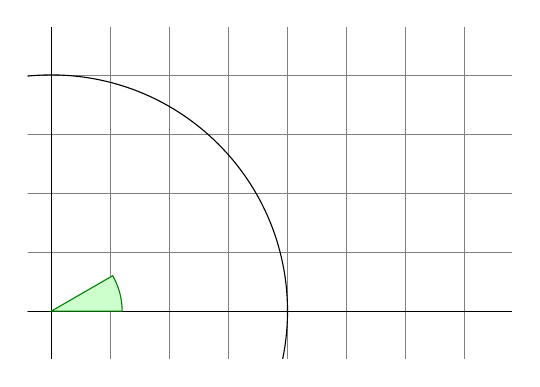
\begin{tikzpicture}[scale=3]
  \clip (-0.1,-0.2)
     rectangle (1.95,1.2);
  \draw[step=.25cm,gray,very thin]
       (-1.4,-1.4) grid (3.4,3.4);
  \draw (-1.5,0) -- (2.5,0);
  \draw (0,-1.5) -- (0,1.5);
  \draw (0,0) circle (1cm);
  \filldraw[fill=green!20!white,
            draw=green!50!black]
    (0,0) -- (3mm,0mm) 
         arc (0:30:3mm) -- cycle;
\end{tikzpicture}
\end{example}
If  you know other programming languages you
may notice the familiar semicolon (\texttt{;}) character that is used
to separate the different commands. With the \ci{usetikzlibrary}
command in the preamble you can enable a wide variety of additional
features for drawing special shapes, like this box which is slightly bent.
\begin{example}
\usetikzlibrary{%
  decorations.pathmorphing}
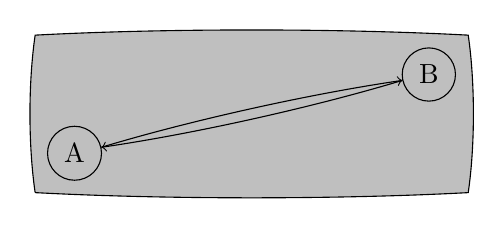
\begin{tikzpicture}[
     decoration={bent,aspect=.3}]
 \draw [decorate,fill=lightgray]
        (0,0) rectangle (5.5,2);
 \node[circle,draw] 
        (A) at (.5,.5) {A};
 \node[circle,draw] 
        (B) at (5,1.5) {B};
 \draw[->,decorate] (A) -- (B);
 \draw[->,decorate] (B) -- (A);
\end{tikzpicture}
\end{example}

You can even draw diagrams that look as if they came straight from a book pascal
programming spruced up with some fancy backgrounds. The code is a bit
more daunting than the example above, so I will just show you the
result of this one.

\begin{center}
\begin{tikzpicture}[point/.style={coordinate},thick,draw=black!50,>=stealth',
                    tip/.style={->,shorten >=1pt},every join/.style={rounded corners},
                    skip loop/.style={to path={-- ++(0,#1) -| (\tikztotarget)}},
                    hv path/.style={to path={-| (\tikztotarget)}},
                    vh path/.style={to path={|- (\tikztotarget)}},
                 terminal/.style={
            rounded rectangle,
            minimum size=6mm,
            very thick,draw=black!50,
            top color=white,bottom color=black!20,
            font=\ttfamily\scriptsize},
                nonterminal/.style={
                       rectangle,
                       minimum size=6mm,
                       very thick,
                       draw=red!50!black!50,         % 50% red and 50% black,
                       top color=white,              % a shading that is white at the top...
                       bottom color=red!50!black!20, % and something else at the bottom
                       font=\itshape\scriptsize}]
\matrix[column sep=4mm] {
  % First row:
  & & & & & & & & & & & \node (plus) [terminal] {+};\\
  % Second row:
  \node (p1) [point] {}; &     \node (ui1)    [nonterminal] {unsigned integer}; &
  \node (p2) [point] {}; &     \node (dot)    [terminal]    {.};                &
  \node (p3) [point] {}; &     \node (digit) [terminal]     {digit};            &
  \node (p4) [point] {}; &     \node (p5)     [point] {};                       &
  \node (p6) [point] {}; &     \node (e)      [terminal]    {E};                &
  \node (p7) [point] {}; &                                                      &
  \node (p8) [point] {}; &     \node (ui2)    [nonterminal] {unsigned integer}; &
  \node (p9) [point] {}; &     \node (p10)    [point]       {};\\
  % Third row:
  & & & & & & & & & & & \node (minus)[terminal] {-};\\
};
{ [start chain]
  \chainin (p1);
  \chainin (ui1)   [join=by tip];
  \chainin (p2)    [join];
  \chainin (dot)   [join=by tip];
  \chainin (p3)    [join];
  \chainin (digit) [join=by tip];
  \chainin (p4)    [join];
  { [start branch=digit loop]
    \chainin (p3) [join=by {skip loop=-6mm,tip}];
  }
  \chainin (p5)    [join,join=with p2 by {skip loop=6mm,tip}];
  \chainin (p6)    [join];
  \chainin (e)     [join=by tip];
  \chainin (p7)    [join];
  { [start branch=plus]
    \chainin (plus) [join=by {vh path,tip}];
    \chainin (p8)    [join=by {hv path,tip}];
  }
  { [start branch=minus]
    \chainin (minus) [join=by {vh path,tip}];
    \chainin (p8)    [join=by {hv path,tip}];
  }
  \chainin (p8)    [join];
  \chainin (ui2)   [join=by tip];
  \chainin (p9)    [join,join=with p6 by {skip loop=-11mm,tip}];
  \chainin (p10)   [join=by tip];
}
\end{tikzpicture}
\end{center}

\pagebreak
And there is more, if you have to draw plots of numerical data or
functions, you should have a closer look at the  \pai{pgfplot}
package. It provides everything you need to draw plots. It can even
call the external \texttt{gnuplot} command to evaluate actual
functions you wrote into the graph.

%%% Local Variables:
%%% TeX-master: "lshort.tex"
%%% mode: flyspell
%%% TeX-PDF-mode: t
%%% End:

% The Not So Short Introduction to LaTeX
%
% Copyright (C) 1995--2022 Tobias Oetiker, Marcin Serwin, Hubert Partl,
% Irene Hyna, Elisabeth Schlegl and Contributors.
%
% This document is free software: you can redistribute it and/or modify it
% under the terms of the GNU General Public License as published by the Free
% Software Foundation, either version 3 of the License, or (at your option) any
% later version.
%
% This document is distributed in the hope that it will be useful, but WITHOUT
% ANY WARRANTY; without even the implied warranty of MERCHANTABILITY or FITNESS
% FOR A PARTICULAR PURPOSE.  See the GNU General Public License for more
% details.
%
% You should have received a copy of the GNU General Public License along with
% this document.  If not, see <https://www.gnu.org/licenses/>.

% !TEX root = ./lshort.tex
%%%%%%%%%%%%%%%%%%%%%%%%%%%%%%%%%%%%%%%%%%%%%%%%%%%%%%%%%%%%%%%%%
% Contents: Customising LaTeX output
% $Id$
%%%%%%%%%%%%%%%%%%%%%%%%%%%%%%%%%%%%%%%%%%%%%%%%%%%%%%%%%%%%%%%%%
\chapter{Customising \LaTeX}\label{chap:custom}

\begin{intro}
  Documents produced with the commands you have learned up to this
  point will look acceptable to a large audience. While they are not
  fancy-looking, they obey all the established rules of good
  typesetting, which will make them easy to read and pleasant to look at.

  However, there are situations where \LaTeX{} does not provide a
  command or environment that matches your needs, or the output
  produced by some existing command may not meet your requirements.

  In this chapter, I will try to give some hints on
  how to teach \LaTeX{} new tricks and how to make it produce output
  that looks different from what is provided by default.
\end{intro}

\section{New Commands, Environments and Packages}

At the beginning of this book we have mentioned that \LaTeX{} allows us to
write documents using logical markup, with commands like \csi{emph} or \csi{section}. There
may be however situations where \LaTeX{} does not provide an appropriate command for the content you want to write about.
You may have noticed that all the
commands I introduce in this book are typeset in a box, and that they show up
in the index at the end of the book. There is no \LaTeX{} markup to format example code or commands, but \LaTeX{} allows me to define my own commands for this purpose. I
can write:

\begin{example}
\begin{lscommand}
  \csi{dum}
\end{lscommand}
\end{example}

In this example, I am using both a new environment called
\ei{lscommand}, which is responsible for drawing the box around the
command, and a new command named \csi{csi}, which typesets the command
name and makes a corresponding entry in the index. Check
this out by looking up the \csi{dum} command in the index at the back
of this book, where you'll find an entry for \csi{dum}, pointing to
every page where I mentioned the \csi{dum} command.

If I ever decide that I do not like having the commands typeset in
a box any more, I can simply change the definition of the
\ei{lscommand} environment to create a new look. This is much
easier than going through the whole document to hunt down all the
places where I have used some generic \LaTeX{} commands to draw a
box around some word.

\subsection{New Commands}\label{sec:new_commands}

You have already learned some basic command creation in
\autoref{sec:simple_commands}. The main command is the
\begin{lscommand}
  \csi{NewDocumentCommand}[name:M, argspec:m, definition:m]
\end{lscommand}
It requires three arguments: the \carg{name} of the command you want to create,
the \carg{argspec} (argument specification) and the \emph{definition} of the
command.

The \carg{argspec} argument specifies the number and types of arguments the
command receives. The two most important types are \cargv{m}, for
\emph{mandatory} and \cargv{o} for \emph{optional}. To create a command that
takes two optional arguments, then two mandatory, then again one optional and
finally three mandatory you would write \cargv{oommommm}. If the \carg{argspec}
argument is empty then the command will take no arguments, as you have already
seen.

This example defines a new command called \csi{tnss}. This is
short for \enquote{The Not So Short Introduction to \LaTeX}. Such a command
could come in handy if you had to write the title of this book over
and over again.

\begin{example}
\NewDocumentCommand{\tnss}{}{%
  The not so Short Introduction
    to \LaTeX}
This is \enquote{\tnss} \ldots{}
\enquote{\tnss}
\end{example}

The next example illustrates how to define a new command that takes two
arguments. In order to refer to the received arguments you use
\mintinline{latex}|#1| for the first argument, \mintinline{latex}|#2| for the
second, and so on.

\begin{example}
\NewDocumentCommand{\txsit}{mm}
 {This is the \emph{#1}
  #2 Introduction to \LaTeX}

% in the document body:
\txsit{not so}{short}

\txsit{very}{long}
\end{example}

If your command accepts an optional argument, but the user does not supply one,
a special marker \cargv{-NoValue-} will be inserted instead.
\begin{example}
\NewDocumentCommand{\txsit}{om}
{This is the \emph{#1}
  #2 Introduction to \LaTeX}

% in the document body:
\txsit{definitive}

\txsit[very]{long}
\end{example}
In order to test whether the user supplied a value, use
\begin{lscommand}
  \csi{IfValueTF}[argument:m, value version:m, no value version:m]
\end{lscommand}
macro.
\begin{example}
\NewDocumentCommand{\MyCommand}{o}{
  \IfValueTF {#1} {
    Optional argument: #1.
  } {
    No optional argument given.
  }%
}

\MyCommand\\
\MyCommand[hello]
\end{example}

There are two variations of it: \csi{IfValueT} and \csi{IfValueF} which may
be used if you only need output for one of the branches. The example with
\cargv{-NoValue-} in the output could be fixed by writing
\begin{example}
\NewDocumentCommand{\txsit}{om}
{This is the
  \IfValueT{#1}{\emph{#1} }%
  #2 Introduction to \LaTeX}

% in the document body:
\txsit{definitive}

\txsit[very]{long}
\end{example}
The commands \csi{IfNoValueTF}, \csi{IfNoValueT} and \csi{IfNoValueF}
work exactly the same, but the value\slash{}no-value branches are swapped.

Often you will want to use optional arguments when present but use some default
values when the user does not provide them. This could be achieved by
\csi{IfValueTF}, but with the \cargv{O} argument a default value can be set directly.
It works like \cargv{o} but allows setting a default
if no value is supplied. Write

\begin{example}
\NewDocumentCommand{\txsit}{O{not so}m}
{This is the \emph{#1}
  #2 Introduction to \LaTeX}

% in the document body:
\txsit{definitive}

\txsit[very]{long}
\end{example}

Another useful argument specification is \cargv{s}, short for star. This
argument allows providing different definitions based on whether the
starred or non-starred version of command was issued by the user. It uses
\csi{IfBooleanTF} command (and its variations\csih{IfBooleanT}\csih{IfBooleanF})
that works like the \csi{IfValueTF} command.

\begin{chktexignore}
  \begin{example}
\NewDocumentCommand{\txsit}{sO{not so}m}
{This is the \emph{#2}
  #3 Introduction to \LaTeX%
  \IfBooleanT{#1}{%
    : Superstar Edition%
  }%
}

% in the document body:
\txsit{long}\\
\txsit*{long}
\end{example}
\end{chktexignore}

These are just the most common argument specifications. For a full description,
take a look at the~\cite{usrguide3}.

As we have discussed in \autoref{sec:simple_commands}, \LaTeX{} will not allow
you to create a new command that would overwrite an existing one, you can do so
using \csi{RenewDocumentCommand}. It uses the same argument specification
syntax as the \csi{NewDocumentCommand} command.

In some cases you might want to use the \csi{ProvideDocumentCommand} command.
It works like \csi{NewDocumentCommand}, but if the command is already defined,
\LaTeX{} will silently ignore the new definition. Yet another variant is the
\csi{DeclareDocumentCommand}. It always creates the given command, overwriting
old definition if it exists.

\subsection{New Environments}
The \csi{NewDocumentEnvironment} command lets you create your own environments. It has the
following syntax:

\begin{lscommand}
  \small
  \csi{NewDocumentEnvironment}[name:m, argspec:m, at begin:m, at end:m]
\end{lscommand}
The \carg{argspec} argument is the same as in the
\csi{NewDocumentCommand} command. The contents of \carg{at begin} and \carg{at
  end} arguments will be inserted respectively when the commands
\csi{begin}[name: m] and \csi{end}[name: m] is encountered. The example
presented in \autoref{lst:kingenv} illustrates the usage of this command.
\begin{listing}
  \begin{example}
\NewDocumentEnvironment{king}{}{%
  \emph{Listen! For the
    king made a statement:}%
  \\[1em]%
} {%
  \\[1em]%
  \emph{This concludes
    the king's statement.}%
}

\begin{king}
My humble subjects \ldots
\end{king}
\end{example}
  \caption{An example of using \csi{NewDocumentEnvironment}
    command.}\label{lst:kingenv}
\end{listing}

Note that when environment argument are read, they are read \emph{after} the
\csi{begin}[name: m] command. This may be especially counterintuitive when we
consider the \cargv{s} specification. \autoref{lst:kingsenv} illustrates this.
\begin{listing}
  \begin{example}
\NewDocumentEnvironment{king}{s}{%
  \IfBooleanTF{#1}{
    \begin{center}
      \emph{Thus spoke Charles I:}
      \\[1em]%
    \end{center}%
  } {
    \emph{Listen! For the
      king made a statement:}%
      \\[1em]%
  }%
} {%
  \\[1em]%
  \emph{This concludes
    the king's statement.}%
}

\begin{king}*
My humble subjects \ldots
\end{king}
\end{example}
  \caption{An example of using the \cargv{s} specifier when defining a new
    environment.}\label{lst:kingsenv}
\end{listing}
If you want to create a starred version of an environment (similar to the
\hologo{AmSLaTeX} environments) you have to define it separately.
\begin{minted}{latex}
\NewDocumentEnvironment{king}{moo} { ... } { ... }
\NewDocumentEnvironment{king*}{moo} { ... } { ... }
\end{minted}
Obviously you can use the same internal commands to define them, for example
renaming the previous implementation to \cargv{kinginternal} making the
\cargv{king} and \cargv{king*} a thin wrapper around it.

The \csi{NewDocumentEnvironment} also introduces a special argument
specification: \cargv{+b}, short for body.\footnote{The \cargv{+} indicates
  that it may contain multiple paragraphs.} It is only allowed as the last
argument in the \carg{argspec}. It allows you to receive the body of the
environment as an argument.
\begin{example}
\NewDocumentEnvironment{twice}{+b} {%
  First time:\\ #1

  Second time:\\ #1
} {}

\begin{twice}
This will be printed twice!
\end{twice}
\end{example}
While this makes one of the \carg{at begin}, \carg{at end} arguments redundant,
they are still required. (In the example above we provided an empty \carg{at
  end}.)

Do not overuse \cargv{+b} as this will both add limitations to the environments
like \csi{verb} not being allowed inside and it will slow down the
typesetting.

Similar to the \csi{NewDocumentCommand}, \LaTeX{} makes sure that you do not
define an environment that already exists. If you ever want to change an
existing environment, use the \csi{RenewDocumentEnvironment} command. Its
arguments are the same as the \csi{NewDocumentEnvironment} command.

\subsection{Copying commands}\label{sec:copyingcommands}

When redefining commands you may want to use the original version of the
command. Your initial code may look like this
\begin{minted}{latex}
\RenewDocumentCommand{\emph}{m}{%
  \emph{#1}~(\enquote{#1} is emphasised)%
}
\end{minted}
but when you try to compile the document you will get the error message
\begin{verbatim}
! TeX capacity exceeded, sorry [input stack size=5000].
\end{verbatim}

To understand why this happens it is instructive to consider how \TeX{} expands
the defined commands. The above \csi{RenewDocumentCommand} tells the \TeX{}
engine that whenever \csi{emph}[foo:vm] is seen it must replace it with
\mintinline{latex}|\emph{foo}~(\enquote{foo} is emphasised)|. You may already see the
problem here. In the next stage it will again replace the \csi{emph}[foo:vm]
yielding
\begin{minted}[breaklines]{latex}
\emph{foo}~(\enquote{foo} is emphasised)~(\enquote{foo} is emphasised)
\end{minted}
This process will never end and at some point \TeX{}
simply gives up.

Note that
\begin{minted}{latex}
\NewDocumentCommand{\oldemph}{m}{\emph{#1}}
\RenewDocumentCommand{\emph}{m}{%
  \oldemph{#1}~(\enquote{#1} is emphasised)%
}
\end{minted}
will suffer the same fate since \mintinline{latex}|\oldemph{...}| %chktex 11 
will  be replaced by \TeX{} with \mintinline{latex}|\emph{...}| and %chktex 11
the  cycle repeats.

In order to avoid this problem a special command exists
\begin{lscommand}
  \csi{NewCommandCopy}[name:M, command:M]
\end{lscommand}
It makes the \carg{name} the exact copy of the \carg{command}. The following example shows how this works
\begin{example}[examplewidth=0.35\linewidth]
\NewDocumentCommand{\foo}{}{Batman!}

\NewDocumentCommand{\newfoo}{}{\foo}
\NewCommandCopy{\copiedfoo}{\foo}

\RenewDocumentCommand{\foo}{}{Na Na Na}

\foo{} \newfoo{} \copiedfoo{}
\end{example}

This is precisely the behaviour we need in order to redefine the \csi{emph}
command as we have tried to do earlier.
\begin{example}[examplewidth=0.35\linewidth]
\NewCommandCopy{\oldemph}{\emph}
\RenewDocumentCommand{\emph}{m}{%
  \oldemph{#1}~(\enquote{#1}
  is emphasised)%
}

And here it \emph{comes}.
\end{example}

\subsection{Command-line \LaTeX}

If you work on a Unix-like OS, you might be using Makefiles to build your
\LaTeX{} projects. In that connection it might be interesting to produce
different versions of the same document by calling \LaTeX{} with command-line
parameters. If you add the following structure to your document:

\begin{minted}{latex}
\IfBooleanTF{\blackandwhite} {
  % "black and white" mode; do something...
} {
  % "color" mode; do something different...
}
\end{minted}

Now compile document like this:
\begin{verbatim}
xelatex '\NewCommandCopy{\blackandwhite}{\BooleanTrue}
    \input{test.tex}'
\end{verbatim}
First the command \verb|\blackandwhite| is defined as the \csi{BooleanTrue} macro which
holds a special value used in \csi{IfBooleanTF} checks. Then the actual file is
read with input. By setting \verb|\blackandwhite| to \csi{BooleanFalse} the
colour version of the document would be produced.

\subsection{Your Own Package}

If you define a lot of new environments and commands, the preamble of
your document will get quite long. In this situation, it is a good
idea to create a \LaTeX{} package containing all your command and
environment definitions. Use the \csi{usepackage}
command to make the package available in your document.

\begin{listing}
  \begin{lined}{\textwidth}
    \begin{minted}{latex}
\ProvidesExplPackage{demopack}{2022-05-05}{0.1}{%
  Package by Tobias Oetiker
}

\NewDocumentCommand{\tnss}{} {
  The~not~so~Short~Introduction~to~\LaTeX
}
\NewDocumentCommand{\txsit}{O{not~so}} {
  The~\emph{#1}~Short~Introduction~to~\LaTeX
}

\NewDocumentEnvironment{king}{} {
  \begin{quote}
} {
  \end{quote}
}
\end{minted}
  \end{lined}
  \caption{Example Package.}\label{package}
\end{listing}

Writing a package basically consists of copying the contents of your document
preamble (with minor adjustments) into a separate file with a name ending in
\texttt{.sty}. There is one special command,
\begin{lscommand}
  \csi{ProvidesExplPackage}[name:m, date:m, version:m, description:m]
\end{lscommand}
for use at the very beginning of your package file. This command tells the
\LaTeX{} to process the  file in \emph{expl mode}. The most visible effect of
this is that all whitespace is ignored. You may have noticed that in many of
the examples above we had to end most lines with \ai{\%} to get correct spacing
in the output. In \emph{expl mode}, spaces have to be added explicitly if
needed at all. They are usually quite rare when writing a package. To insert
spaces, use the \ai{\~} character, which normally denotes non-breaking
space.\footnote{If you want to insert non-breaking space in \emph{expl mode},
  use \csi{nobreakspace}.} Paragraphs can be started with the \csi{par} command.

The arguments are used to provide information about package in the log file. If
you use this package and look at the log file you will find
\begin{verbatim}
Package: demopack 2022-05-05 v0.1 Package by Tobias Oetiker
\end{verbatim}
in the \eei{.log} file.

\csi{ProvidesExplPackage} will also issue a sensible error message when you try
to include a package twice. \autoref{package} shows a small example package
that contains the commands defined in the examples above.

\section{Fonts and Sizes}\label{sec:fontsize}

\subsection{Font Changing Commands}\index{font}\index{font size}

\LaTeX{} fonts are influenced by four parameters
\begin{description}
  \item[family] The collection of fonts. For example, \enquote*{Latin Modern
      Roman} or \enquote*{Source Code Pro}.
  \item[series] The weight of the font. For example, \enquote*{bold} or
    \enquote*{medium}.
  \item[shape] The shape of glyphs within a font family. For example,
    \enquote*{small caps} or \enquote*{italics}.
  \item[size] The size of the glyphs. For example, \enquote*{\qty{10}{pt}} or
    \enquote*{\qty{12}{pt}}.
\end{description}
\LaTeX{} automatically chooses the appropriate font family, series, shape and
size based on the logical structure of the document (sections, footnotes,
emphasis, \ldots). It is possible however to instruct \LaTeX{} manually which
font to use. It is important to note that not every combination of
family\slash{}series\slash{}shape exists as an actual font. \LaTeX{} will
complain if you try for something that does not exist.

\LaTeX{} predefines three font families to use throughout the document: the
upright or roman family accessible via \csi{textrm}, the \textsf{sans serif
  family} accessible via \csi{textsf} and monospace or typewriter family
accessible via \csi{texttt}.
\begin{example}
\textrm{Roman is the default
  in articles.} \\
\textsf{Sans serif is used in
  presentations.} \\
\texttt{Monospace is used in
  verbatim code blocks.}
\end{example}

There are only two predefined \LaTeX{} series: medium (\csi{textmd}) and bold
(\csi{textbf}).
\begin{example}
\textmd{The default.} \\
\textbf{Bold font.}
\end{example}

Shapes are a bit more complicated. The three basic shapes are: italics
(\csi{textit}), oblique or slanted\footnote{Oblique shape differs from the
  italics in that italic shape uses different glyphs while oblique shape uses
  the same glyphs but slanted. The difference is really obvious
  \fontspec{cmunui.otf} when you look at the unslanted italic
  font.} (\csi{textsl}) and small capitals (\csi{textsc}).
\begin{example}
\textit{Italic shape.} \\
\textsl{Slanted shape.} \\
\textsc{Small Capitals.}
\end{example}
However there are two additional shapes that are not provided by default
\LaTeX{} fonts: swash (\csi{textsw}), for decorative fonts and spaced caps and
small caps (\csi{textssc}). These are rarely used but may come in handy when
using custom fonts as described in \autoref{sec:fontspec}.
\begin{example}
\setmainfont{EB Garamond} %!hide
Question vs. \textsw{Question}
\end{example}
In addition two virtual shapes are provided: upright (\csi{textup}) and
upper-lowercase (\csi{textulc}). These are not actually shapes but utility
commands. The former one switches back to upright font while the latter
disables small capitals. The command \csi{textnormal} is just the combination
of the two.
\begin{example}
\textsl{\textsc{Back to
  \textup{upright.}}} \\
\textsl{\textsc{Back to
  \textulc{lowercase.}}} \\
\textsl{\textsc{Back to
  \textnormal{normal.}}}
\end{example}

All of the commands described above also exist in their switch version. Instead
of receiving the text via argument, they change the font permanently until it is
changed again. For example, the switch version of \csi{textit} and \csi{textrm}
are \csi{itshape} and \csi{rmfamily}, respectively. While the argument versions
are useful for defining commands, switch versions are especially useful when
defining your own environments.
\begin{example}
Only \textit{argument} is
affected. After \itshape
everything is in italics
until \upshape is encountered.
\end{example}
Both argument and switch versions of the described commands are presented in
\autoref{tbl:fonts}.
\begin{table}
  \caption{Default font changing commands of \LaTeX.}\label{tbl:fonts}
  \begin{tabular}{@{}lll@{}}
    \toprule
    Argument Command         & Switch           & Example                      \\
    \midrule
    \csi{textrm}[text:m]     & \csi{rmfamily}   & \textrm{\wi{roman}}          \\
    \csi{textsf}[text:m]     & \csi{sffamily}   & \textsf{\wi{sans serif}}     \\
    \csi{texttt}[text:m]     & \csi{ttfamily}   & \texttt{typewriter}          \\[6pt]
    \csi{textmd}[text:m]     & \csi{mdseries}   & \textmd{medium}              \\
    \csi{textbf}[text:m]     & \csi{bfseries}   & \textbf{\wi{bold face}}      \\[6pt]
    \csi{textup}[text:m]     & \csi{upshape}    & \textup{\wi{upright}}        \\
    \csi{textit}[text:m]     & \csi{itshape}    & \textit{\wi{italic}}         \\
    \csi{textsl}[text:m]     & \csi{slshape}    & \textsl{\wi{slanted}}        \\
    \csi{textsc}[text:m]     & \csi{scshape}    & \textsc{\wi{Small Caps}}     \\
    \csi{textsw}[text:m]     & \csi{swshape}    & \textsw{\wi{Queen of Swash}} \\[6pt]
    \csi{textnormal}[text:m] & \csi{normalfont} & \textnormal{document} font   \\
    \bottomrule
  \end{tabular}
\end{table}

When working with switch versions of fonts that are slanted right it is
important to remember about \wi{italic correction}. This is a small space after
the end of right slanting text that is sometimes necessary to avoid overlapping
letters. It is inserted using \csi{/} command.
\begin{chktexignore}  
\begin{example}
Without: {\itshape oof}bar \\
With: {\itshape oof\/}bar
\end{example}
\end{chktexignore}
The italic correction is handled automatically by the argument versions of the
commands.

In contrast to the previous font changing commands, the size of font can only
be controlled via switch versions. \LaTeX{} predefines some switches for
changing font size, see \autoref{sizes} and \autoref{tab:pointsizes} for their
description.
\begin{table}
  \caption{Commands changing font size.}\label{sizes}\index{font size}
  \begin{tabular}{@{}ll@{\qquad}ll@{}}
    \toprule
    Command                     & Size                             &
    Command                     & Size                               \\
    \midrule
    \csi{tiny}                  & \tiny tiny                       &
    \csi{Large}                 & \Large larger                      \\
    \csi{scriptsize}            & \scriptsize very small           &
    \csi{LARGE}                 & \LARGE very large                  \\
    \csi{footnotesize}          & \footnotesize  quite small       &
    \multirow{2}{*}{\csi{huge}} & \multirow{2}{*}{\huge huge}        \\
    \csi{small}                 & \small small                     &
                                &                                    \\
    \csi{normalsize}            & \normalsize  normal              &
    \multirow{2}{*}{\csi{Huge}} & \multirow{2.2}{*}{\Huge largest}   \\
    \csi{large}                 & \large large                     &
                                &                                    \\
    \bottomrule
  \end{tabular}
\end{table}

\begin{table}
  \caption[Absolute point sizes in standard classes.]{Absolute point sizes in
    standard classes depending on the class option. The default class option is
    \cargv{10pt}.}\label{tab:pointsizes}\label{tab:sizes}
  \sisetup{table-format=2.2}
  \begin{tabular}{@{}lSSS@{}}
    \toprule
                       & \multicolumn{3}{c}{Size (\unit{pt})}                                   \\
    \cmidrule(l){2-4}
    Command            & {\cargv{10pt}}                       & {\cargv{11pt}} & {\cargv{12pt}} \\
    \midrule
    \csi{tiny}         & 5                                    & 6              & 6              \\
    \csi{scriptsize}   & 7                                    & 8              & 8              \\
    \csi{footnotesize} & 8                                    & 9              & 10             \\
    \csi{small}        & 9                                    & 10             & 10.95          \\
    \csi{normalsize}   & 10                                   & 10.95          & 12             \\
    \csi{large}        & 12                                   & 12             & 14.4           \\
    \csi{Large}        & 14.4                                 & 14.4           & 17.28          \\
    \csi{LARGE}        & 17.28                                & 17.28          & 20.74          \\
    \csi{huge}         & 20.74                                & 20.74          & 24.88          \\
    \csi{Huge}         & 24.88                                & 24.88          & 24.88          \\
    \bottomrule
  \end{tabular}
\end{table}

When using these commands it is important to remember that the
line spacing is only updated after the paragraph ends. To avoid putting empty
lines before the closing curly brace you may use the \csi{par} command.
\begin{example}
{\Large Here the line spacing
  is not updated. A bit tight!}

{\Large Much better! I can
  breathe freely again!\par}
\end{example}

An arbitrary font size can be specified using the
\begin{lscommand}
  \csi{fontsize}[size: m, line skip: m]\csi{selectfont}
\end{lscommand}
command combo. The \carg{line skip} determines the height of the text line and
should be usually around \(1.2\) times larger than the \carg{size}.
\begin{example}[vertical_mode, examplewidth=0.7\linewidth]
\fontsize{2cm}{2.4cm}\selectfont A big one!
\end{example}

Fun fact: \LaTeX{} default font is a bit unusual in that it looks slightly
different depending on its size. The difference is presented in the table below
where the text written using different sizes was rescaled to the same height.
\begin{center}
  \begin{tabular}{@{}lll@{}}
    \toprule
    \csi{tiny}                           &
    \csi{normalsize}                     &
    \csi{Huge}                             \\
    \midrule
    \resizebox{!}{2em}{\tiny Text}       &
    \resizebox{!}{2em}{\normalsize Text} &
    \resizebox{!}{2em}{\Huge Text}         \\
    \bottomrule
  \end{tabular}
\end{center}

If you need to access even more font variants and shapes\footnote{For example
  the aforementioned \fontspec{cmunui.otf} upright italic shape.} check out
\citetitle{fntguide}~\cite{fntguide}.

\subsection{Danger, Will Robinson, Danger}

Note! Using explicit font setting commands defies the basic idea of
\LaTeX{} described in \autoref{sec:logical_structure}, which is to separate the
logical and visual markup. The fonts should get switched automatically
according to the requirements of the context. A simple rule of thumb: If you
use the same font changing command in several places in order to typeset a
special kind of information, you should use \csi{NewDocumentCommand} to define
a \enquote{logical wrapper command} for the font changing command.

\begin{example}
\NewDocumentCommand{\oops}{m}{%
 \textbf{#1}}
Do not \oops{enter} this room,
it's occupied by \oops{machines}
of unknown origin and purpose.
\end{example}

This approach has the advantage that you can decide at some later
stage that you want to use a visual representation of danger other
than \csi{textbf}, without having to wade through your document,
identifying all the occurrences of \csi{textbf} and then figuring out
for each one whether it was used for pointing out danger or for some other
reason.

\subsection{Advice}

To conclude this journey into the land of fonts and font sizes,
here is a little word of advice:\nopagebreak

\begin{quote}
  \underline{\textbf{Reme\(\mathfrak{mber}\)\Huge!}} \textit{The}
  \textsf{M\textbf{\LARGE O} \(\mathcal{R}\)\textsl{E}} fonts \Huge you
  \tiny use \footnotesize \textbf{in} a \small \texttt{document},
  \large \textit{the} \normalsize more \textsc{readable} and
  \textsl{\textsf{beautiful} it bec\large o\Large m\LARGE e\huge s}.
\end{quote}

\section{Custom Fonts with \pai{fontspec}}\label{sec:fontspec}

In the following examples we use Adobe Source fonts~\cites{sourceserif,
  sourcesans, sourcecodepro}. These fonts are included with \TeXLive{} \LaTeX{}
distributions and should be available in the directory
\begin{code}
  \nolinkurl{.../texmf-dist/fonts/opentype/adobe}
\end{code}
where the \cargv{...} denotes the install-path of \TeXLive{}.
\hologo{LuaTeX} checks this directory automatically, so it should work fine,
but if you are using \hologo{XeTeX} you must first install these fonts in your
system. You can also download and install them manually from the links provided
in the bibliography. Alternatively swap out their respective names with some other
fonts installed in your system.

Many free OpenType fonts are available at \url{https://fontlibrary.org/}.

\subsection{Main Document Fonts}

If you are not pleased with the default Latin Modern font, you can change it to
any font installed in your system using the \pai*{fontspec} package. It provides
three main commands for changing document fonts:
\begin{lscommand}
  \csi{setmainfont}[options: o, font: m] \\
  \csi{setsansfont}[options: o, font: m] \\
  \csi{setmonofont}[options: o, font: m]
\end{lscommand}
This commands change, respectively, the main font of the document, \textsf{the
  sans serif font used in the document} and \texttt{the monospace font in the
  document}.
\begin{example}
Normal text.
  \emph{Emphasised.} \\
\textsf{Sans serif text.
  \emph{Emphasised}.} \\
\texttt{Monospace text.
  \emph{Emphasised}.} \\

\setmainfont{Source Serif Pro}
\setsansfont{Source Sans Pro}
\setmonofont{Source Code Pro}
Normal text.
  \emph{Emphasised.} \\
\textsf{Sans serif text.
  \emph{Emphasised}.} \\
\texttt{Monospace text.
  \emph{Emphasised}.}
\end{example}
Note that it is best to put these commands in the preamble of your document,
because some fonts are frozen when the body starts.

The optional \carg{options} argument accepts key value lists that allow to
customise the font features. For example, many fonts contain,
old style numerals that are not used by default. You can pass
\cargv{Number=OldStyle} if you want to use them in your document.
\begin{example}
\setmainfont{Source Serif Pro}
0123456789

\setmainfont[
  Numbers=OldStyle,
]{Source Serif Pro}
0123456789
\end{example}

Some fonts also provide special glyphs for a given language. For example the
Latin Modern Font provides a special
\enquote{\setmainfont[Language=Polish]{Latin Modern Roman}fk} ligature for the
Polish language. You can set the \cargv{Language} key to a given language to
enable these features.
\begin{example}
agrafka

\setmainfont[
  Language=Polish,
]{Latin Modern Roman}
agrafka
\end{example}
The \pai{polyglossia} package activates these features automatically so you
don't have to worry about them if you use it.

If your font supports it you may wish to enable automatic fractions insertion
with \cargv{Fractions=On} key.
\begin{example}
1/2 3/4 123/456

\setmainfont[
  Fractions=On,
]{Latin Modern Roman}
1/2 3/4 123/456

\setmainfont[
  Fractions=On,
]{Source Serif Pro}
1/2 3/4 123/456
\end{example}

The OpenType font format defines a lot of more font features, that may or may not
be supported by your font of choice. Consult with the \pai*{fontspec} package
documentation for a comprehensive description and examples.

\subsection{Specifying Fonts via Filenames}\label{ssec:fonts_filename}

If you do not want to install fonts in your system or you are working on a
collaborative project where not everybody has the necessary fonts installed on their system,
you can add font files to your project and specify the fonts directly via their filenames.
In this case you must specify
font variations manually. Because the filenames are usually very similar, it is
possible to enter them using \cargv{*} patterns, where \cargv{*} is replaced by
the main name defined. Extension may also be passed via the \cargv{Extension}
key to avoid repetition. See \autoref{lst:fontloading} for a comparison of font
loading techniques. If the font files are not present in the same directory as
the document you may have to specify it directly using the \cargv{Path} key.
\begin{listing}
  \begin{example}[vertical_mode, examplewidth=0.8\linewidth]
\setmainfont{Source Serif Pro}
Normal text. \textit{Italics.} \textbf{Bold.}
\textit{\textbf{Bold italics.}} \\

\setmainfont{SourceSerifPro-Regular.otf}
Normal text. \textit{Italics.} \textbf{Bold.}
\textit{\textbf{Bold italics.}} \\
 
\setmainfont[
  ItalicFont=SourceSerifPro-RegularIt.otf,
  BoldFont=SourceSerifPro-Bold.otf,
  BoldItalicFont=SourceSerifPro-BoldIt.otf,
]{SourceSerifPro-Regular.otf}
Normal text. \textit{Italics.} \textbf{Bold.}
\textit{\textbf{Bold italics.}} \\

\setmainfont[
  Extension=.otf,
  UprightFont=*-Regular,
  ItalicFont=*-RegularIt,
  BoldFont=*-Bold,
  BoldItalicFont=*-BoldIt,
]{SourceSerifPro}
Normal text. \textit{Italics.} \textbf{Bold.}
\textit{\textbf{Bold italics.}}
\end{example}
  \caption{Comparison of font loading with the \pai{fontspec}
    package.}\label{lst:fontloading}
\end{listing}

The default \LaTeX{} fonts are rather atypical in that they distinguish between
\textit{italics} and \textsl{slanted} font. Most fonts do not do this, so
\pai{fontspec} defines slanted font to be the same as italics. This may be
fixed by setting the \cargv{SlantedFont} key explicitly.
\begin{example}[vertical_mode, examplewidth=0.7\linewidth]
\setmainfont{Latin Modern Roman}
\textit{italics} vs. \textsl{slanted}

\setmainfont[
  SlantedFont=Latin Modern Roman Slanted,
]{Latin Modern Roman}
\textit{italics} vs. \textsl{slanted}
\end{example}

\subsection{Defining New Fonts}

So far we have only talked about changing the fonts for the whole document. It
is possible however to define new fonts that are used only sporadically
throughout the document, for emphasis or decorative purposes. It is possible to
do so using the
\begin{lscommand}
  \csi{newfontfamily}[command: M, options: o, font: m]
\end{lscommand}
It defines new \carg{command} that works like to the \csi{rmfamily} or
\csi{sffamily} commands.
\begin{example}
\newfontfamily{\sourcefamily}[
  Numbers=OldStyle,
]{Source Serif Pro}

Normal text when suddenly
\ldots{} \sourcefamily
a different font! 0123456789
\end{example}
This is especially useful when working with multiple languages as you have
already seen in \autoref{sec:polyglossia}.

The \csi{newfontfamily} checks whether the font family is already defined and
raises an error if it is. As in \autoref{sec:new_commands} the
\csi{renewfontfamily} and \csi{providefontfamily} are available if you want to
redefine existing font families.

\subsection{Math Fonts}\label{sec:math_fonts}

The package \pai{unicode-math}, introduced in \autoref{chap:math}, uses
\pai{fontspec} under the hood and already enables you to use any OpenType math
font within your document. The main command to do so is called
\csi{setmathfont}. It accepts either a font name or a filename. In contrast to
the text fonts that often consist of multiple files, math fonts typically
consist of a single file, thus specifying it via a filename is not as
complicated as presented in \autoref{ssec:fonts_filename}.
\begin{code}
  \begin{minted}{latex}
\setmathfont{STIX Two Math}
  \end{minted}
\end{code}
is equivalent to
\begin{code}
  \begin{minted}{latex}
\setmathfont{STIXTwoMath-Regular.otf}
  \end{minted}
\end{code}
and the latter works in both \hologo{LuaLaTeX} and \hologo{XeLaTeX}. While
changing math fonts throughout the document is possible, it may lead to some
problems; prefer to set them in the preamble for the whole document.
\begin{example}[standalone, paperheight=2.5cm, paperwidth=6cm]
\usepackage{unicode-math}%!hide
\setmainfont{EB Garamond}
\setmathfont{Garamond Math}
% ...

\begin{document} %!hide
\noindent %!hide
Now we are using Garamond fonts.
\[
  \symrm{e}^{\symrm{\pi}
    \symrm{i}} + 1 = 0 \quad
  \sum_{i=0}^\infty \iint_a^b
  \lim_{h\to0}\frac{\sqrt[3]{
    \symbb{A}}}{2^h}\,\symrm{d}x
\]
\end{document}%!hide
\end{example}

Not all math fonts have the same character coverage. For example, the default
font doesn't have lowercase script letters. If you don't want to switch the
fonts entirely but just use some characters from a different font, you
can use the \cargv{range} key in the options to the \csi{setmathfont} command.
\begin{example}[standalone, paperheight=1cm, paperwidth=6cm]
\usepackage{unicode-math}%!hide
\begin{document} %!hide
\noindent %!hide
\(xyz = \symscr{Hello}\) vs.\
\setmathfont[
  range=scr,
]{STIX Two Math}
\(xyz = \symscr{Hello}\)
\end{document}%!hide
\end{example}
You can also set it to exact Unicode ranges if you need more control over
replaced symbols.

Some fonts define two types of script font \emph{roundhand} and \emph{chancery}. These are
normally available as the first stylistic set feature of the font. You can map
\csi{symcal} which is normally a synonym for \csi{symscr}, to produce the
alternative script letters.
\begin{example}[standalone, paperheight=1cm, paperwidth=6cm]
\usepackage{unicode-math}%!hide
\begin{document} %!hide
% TODO: Waiting for unicode-math fix
\setmathfont{STIX Two Math}
\setmathfont[
  range={cal, bfcal},
  StylisticSet=1,
]{STIX Two Math}

\noindent %!hide
\(\symscr{ABCDabcd}\) vs.\
\(\symcal{ABCDabcd}\) 
\end{document}%!hide
\end{example}

The default behaviour of the \csi{not} command, is to combine the negating glyph
with the following symbol. This usually produces satisfactory results. If the
font defines a dedicated negated symbol it is probably better to use it in such
situations. The \csi{not} command is able to use a predefined mapping to use
such glyphs based on the negated symbol. If the default mapping does not
contain the combination, or if you prefer to use a different negation you can
create a new mapping by using \csi{NewNegationCommand}.
\begin{example}
\(\not\cong\) vs.\
\NewNegationCommand{%
    \cong}{\simneqq}%
\(\not\cong\)
\end{example}

\section{Colours}\label{sec:colors}\index{colours}

\subsection{Coloured Text}
In the \autoref{sec:logical_structure} we have used different text colours to
illustrate an example. These can be obtained with the \pai*{xcolor} package. It
provides three commands to change the colour of text:
\begin{lscommand}
  \csi{color}[model: o, color: m] \\
  \csi{textcolor}[model: o, color: m, text: m]
  \csi{mathcolor}[model: o, color: m, text: m]
\end{lscommand}
The \csi{color} is a switch version while \csi{textcolor} and \csi{mathcolor}
only apply to their argument. If no \carg{model} is specified, then
\carg{color} is specified as colour expression. The simplest colour expression
is just the name of the colour, for example \cargv{yellow} or \cargv{red}.
\begin{example}
\textcolor{yellow}{foo} \\
\color{red} baz
\[
  \mathcolor{blue}{
    \sum_{k=0}
  }^{10} i
\]
\end{example}
The list of predefined colours can be found in \autoref{tbl:basecolors}. You can
also pass \cargv{dvipsnames}, \cargv{svgnames} or \cargv{x11names} as a package
options to extend the predefined colours. Consult the package documentation for
a full list.
\begin{table}
  \ExplSyntaxOn
  \NewDocumentCommand{\DemoColor}{m}{
    \raisebox{0.15cm}{\cargv{#1}} &
    \fcolorbox{black}{#1}{\phantom{\rule{0.5cm}{0.5cm}}}
  }
  \ExplSyntaxOff
  \caption{Basic colours predefined by the \pai{xcolor}
    package.}\label{tbl:basecolors}
  \begin{tabular}{@{}lc*2{@{\qquad}lc}@{}}
    \toprule
    Name                 & Demo                  &
    Name                 & Demo                  &
    Name                 & Demo                                       \\
    \midrule
    \DemoColor{black}    & \DemoColor{lightgray} & \DemoColor{purple} \\
    \DemoColor{blue}     & \DemoColor{lime}      & \DemoColor{red}    \\
    \DemoColor{brown}    & \DemoColor{magenta}   & \DemoColor{teal}   \\
    \DemoColor{cyan}     & \DemoColor{olive}     & \DemoColor{violet} \\
    \DemoColor{darkgray} & \DemoColor{orange}    & \DemoColor{white}  \\
    \DemoColor{gray}     & \DemoColor{pink}      & \DemoColor{yellow} \\
    \DemoColor{green}    &                       &                    \\
    \bottomrule
  \end{tabular}
\end{table}

Another type of colour expression is a mix of two colours. The syntax is
\begin{code}
  \cargv{\carg{first color}!\carg{percentage}!\carg{second color}}.
\end{code}
The resulting colour will be the result of mixing
\qty[parse-numbers=false]{\carg{percentage}}{\percent} of the \carg{first
  color} and \qty[parse-numbers=false]{100-\carg{percentage}}{\percent} of the
\carg{second color}. If you omit the \carg{second color} it defaults to white.
\begin{example}
\textcolor{green!100!red}{C}%
\textcolor{green!80!red}{o}%
\textcolor{green!60!red}{l}%
\textcolor{green!40!red}{o}%
\textcolor{green!20!red}{r}%
\textcolor{green!0!red}{s} \\
\textcolor{blue!100}{B}%
\textcolor{blue!75}{l}%
\textcolor{blue!50}{u}%
\textcolor{blue!25}{e}
\end{example}
Colour mixing is left associative so
\begin{code}
  \cargv{\carg{A}!\carg{n}!\carg{B}!\carg{m}!\carg{C}}
\end{code}
means calculate the mixture of \carg{A} and \carg{B} and then mixture of the
result and \carg{C}. You can also use the minus sign before the expression to
get the complementary colour.
\begin{example}
\color{green!20!red!60!blue}
\LaTeX{} \\
\color{-green!20!red!60!blue}
\LaTeX{}
\end{example}

\subsection{Models}

While colour mixing via expression is useful for simple colour specification, it
is often the case that we want to use colour that is defined in terms of its RGB
or HSB values. Different input method colours can be specified using the optional
\carg{model} argument. Note that it is case-sensitive.

The simplest model is \cargv{Gray}. It accepts a single number from \(0\)to
\(15\) and produces a grey colour with the given brightness.
\begin{example}
\textcolor[Gray]{0}{Zero}    \\
\textcolor[Gray]{3}{Three}   \\
\textcolor[Gray]{7}{Seven}   \\
\textcolor[Gray]{11}{Eleven} \\
\textcolor[Gray]{15}{Fifteen}
\end{example}

You can input RGB values in three ways: \cargv{rgb}, \cargv{RGB} and
\cargv{HTML} models. The \cargv{HTML} model accepts a hexadecimal colour code.
The code may be either upper or lowercase.
\begin{example}
\textcolor[HTML]{e63946}{e63946}
\textcolor[HTML]{06D6A0}{06D6A0}
\end{example}
The \cargv{rgb} model accepts three decimal numbers, each between \(0\) and
\(1\), while the \cargv{RGB} model accepts three integers from \(0\) to \(255\).
\begin{example}
\textcolor[RGB]{255, 204, 102}{
  255, 204, 102
} \\
\textcolor[rgb]{0.4, 0.4, 1.0}{
  0.4, 0.4, 1.0
}
\end{example}

If you prefer the subtractive colour model, both \cargv{cmy} and \cargv{cmyk} are
available. They accept decimal numbers between \(0\) and \(1\) to specify
the amount of each colour.
\begin{example}
\textcolor[cmy]{0.7, 0.4, 0.3}{
  0.7, 0.4, 0.3
} \\
\textcolor[cmyk]{
  0.7, 0.4, 0.3, 0.5
}{
  0.7, 0.4, 0.3, 0.5
}
\end{example}

There are three models that enable defining colours by HSB\@: \cargv{hsb},
\cargv{Hsb} and \cargv{HSB}. The first two accept three decimal numbers for
each value, the difference being that the \cargv{Hsb} accepts hue as an angle
in degrees, that is a number between \(0\) and \(360\). The \cargv{hsb} accepts
it as a number between \(0\) and \(1\), while saturation and brightness
are passed the same way in both model---as a number between \(0\) and \(1\).
\begin{example}
\textcolor[hsb]{
  0.4, 0.8, 0.75
}{
  0.4, 0.8, 0.75
}\\
\textcolor[Hsb]{
  144, 0.8, 0.75
}{
  144, 0.8, 0.75
}
\end{example}
The \cargv{HSB} in turn accepts all three as integers---each between \(0\) and
\(240\).
\begin{example}
\textcolor[HSB]{
  144, 200, 120
}{
  144, 200, 120
}
\end{example}

If you are writing a paper about light you may also find that the \cargv{wave}
model comes in handy. It allows you to specify a colour by its wavelength. It
accepts a single decimal number that represents a wavelength in visible
spectrum in nanometres.
\begin{example}
\textcolor[wave]{452}{
  If a light has wavelength
  \qty{452}{\nm} it looks
  like this.  
} \\
\textcolor[wave]{700}{
  Light with wavelength above
  \qty{814}{\nm} is called
  infrared.
}
\end{example}

\subsection{Defining Your Own Colours}

If you want to use a given colour more than once it makes sense to define
it as a macro. While you could use the \csi{NewDocumentCommand} to define it,
the \pai{xcolor} package provides a better way via the
\begin{lscommand}
  \csi{definecolor}[name: m, model: m, value: m].
\end{lscommand}
command. Using it makes it possible to use the newly defined colour in colour
mixing and such.
\begin{example}
\definecolor{MyRed}{wave}{712}
\textcolor{MyRed}{MyRed is
  the perfect colour for you!}
\textcolor{MyRed!60}{Tints
  are also available!}
\end{example}
Be careful though, since it doesn't guard against redefinition. If you want to
check whether you haven't redefined some colour put \csi{tracingcolors} in your
preamble. This will produce warnings when redefinition happens.

If you want to make sure a colour is present but don't want to redefine it if it
already exists then \csi{providecolor} does exactly that. There is also
\csi{colorlet} that simply creates a copy of a given colour similar to the
\csi{NewCommandCopy} command.

Colours defined in different models may need to be converted when mixing them.
This may lead to a situation where \mintinline{latex}|\color{a!75!b}| will
result in different colour than \mintinline{latex}|\color{b!25!a}|. Keep that in
mind when mixing your own colours.

\subsection{Colourful Pages and Boxes}

So far we have only considered changing the text colour. It is however possible
to also change the background colour of the document page. To do this use the
\begin{lscommand}
  \csi{pagecolor}[model: o, color: m]
\end{lscommand}
command, which accepts the same arguments as the \csi{color} command. If you
want to revert to the default transparent background you may do so with the
\csi{nopagecolor} command.
\begin{example}[standalone, paperheight=1cm]
\usepackage{xcolor} %!hide
\begin{document} %!hide
\pagecolor{orange} \color{-orange}
Small is colourful \ldots?
\end{document} %!hide
\end{example}

If you only want to specify a background of some text instead of the whole page
you can use the
\begin{lscommand}
  \csi{colorbox}[model: o, color: m, text: m] \\
  \csi{fcolorbox}[model: o, color: m, model: o, color: m, text: m]
\end{lscommand}
commands. The first one only colours the background, while the second one
allows also drawing a frame (the \enquote*{f} stands for \enquote{framed}).
\begin{example}
It is \colorbox{gray}{curious}
how much a document can be
enhanced or ruined by
\fcolorbox{blue}{red}{
  colours.
}
\end{example}
Boxes are explored further in \autoref{sec:boxes}.

\section{Lengths and Spacing}

\subsection{\LaTeX{} Units}\index{units (\TeX)}\index{dimensions}%
\label{sec:dimensions}
\begingroup
\DeclareSIUnit{\in}{in}
\DeclareSIUnit{\pt}{pt}
\DeclareSIUnit{\bp}{bp}
\DeclareSIUnit{\sp}{sp}
\DeclareSIUnit{\dd}{dd}
\ExplSyntaxOn
\NewDocumentCommand{\DimVal}{m}{
  \num{\dim_to_decimal_in_sp:n {#1}}
}
\NewDocumentCommand{\fnum}{mm}{
  \num[
    number-mode=text,
    parse-numbers=false,
  ]{
    \sfrac{
      \num[number-mode=math,parse-numbers=true]{#1}
    }{
      \num[number-mode=math,parse-numbers=true]{#2}
    }
  }
}

\NewDocumentCommand{\fqty}{mmm}{
  \qty[
    number-mode=text,
    parse-numbers=false,
  ]{
    \sfrac{
      \num[number-mode=math,parse-numbers=true]{#1}
    }{
      \num[number-mode=math,parse-numbers=true]{#2}
    }
  }{#3}
}
\ExplSyntaxOff

Throughout this booklet we have often presented commands that accept length as
one of its parameters such as \csi{\bs} or \csi{fontsize}. When introducing
them we have used \unit{\cm} and \unit{\pt} which stand for centimetre and
point, but these are not the only units available in \LaTeX{}.

The most fundamental unit in \LaTeX{} is \unit{\sp} which stands for
\emph{scaled point}. Its width is equal to \fqty{1}{65536}{\pt}, where
\qty{1}{\pt} is equal to \fnum{1}{72.27} of an international inch which in turn
is defined as exactly \qty{25.4}{\mm}. All units in \TeX{} are ultimately
represented as a whole numbers of \unit{sp}. See \autoref{units} for the exact
values.
\begin{table}
  \caption{\LaTeX{} Units.}\label{units}\index{units}
  \begin{tabular}{@{}clrrl@{}}
    \toprule
    Unit     & Meaning                                                                                                 & Definition            & {Value (\unit{\sp})} & Demo            \\
    \midrule
    \ltx|cm| & centimetre                                                                                              & \qty{0.01}{\m}        & \DimVal{1cm}         & \demowidth{1cm} \\
    \ltx|mm| & millimetre                                                                                              & \qty{0.001}{\m}       & \DimVal{1mm}         & \demowidth{1mm} \\
    \ltx|in| & inch                                                                                                    & \qty{25.4}{\mm}       & \DimVal{1in}         & \demowidth{1in} \\
    \ltx|pt| & point                                                                                                   & \fqty{1}{72.27}{\in}  & \DimVal{1pt}         & \demowidth{1pt} \\
    \ltx|sp| & scaled point                                                                                            & \fqty{1}{65536}{\pt}  & \DimVal{1sp}         & \demowidth{1sp} \\
    \ltx|pc| & pica                                                                                                    & \qty{12}{\pt}         & \DimVal{1pc}         & \demowidth{1pc} \\
    \ltx|dd| & didot                                                                                                   & \qty{0.376065}{\mm}   & \DimVal{1dd}         & \demowidth{1dd} \\
    \ltx|cc| & cicero                                                                                                  & \qty{12}{\dd}         & \DimVal{1cc}         & \demowidth{1cc} \\
    \ltx|nd| & new didot                                                                                               & \qty{0.375}{\mm}      & \DimVal{1nd}         & \demowidth{1nd} \\
    \ltx|bp| & big point                                                                                               & \fqty{1}{72}{\in}     & \DimVal{1bp}         & \demowidth{1bp} \\[6pt]
    \ltx|em| & \multicolumn{3}{m{7cm}}{roughly width of an \enquote*{M} in the current font}                           & \demowidth{1em}                                                \\
    \ltx|ex| & \multicolumn{3}{m{7cm}}{roughly height of an \enquote*{x} in the current font}                          & \demowidth{1ex}                                                \\
    \ltx|mu| & \multicolumn{3}{m{7cm}}{equal to \fqty{1}{18}{em}, where \unit{em} is taken from the current math font} & \demowidth{0.05556em}                                          \\
    \bottomrule
  \end{tabular}
\end{table}

The last three units mentioned in the table are relative to the current font
used. Historically they were related to the \enquote*{M} and \enquote*{x}
glyphs in a given font but today they are arbitrarily set by fonts. These units
are useful if we want the length to scale proportionally when used with
different font sizes. The \mintinline{latex}|em| unit is usually used for
horizontal lengths, while the \mintinline{latex}|ex| is used for vertical
lengths. The \mintinline{latex}|mu| unit can only be used in math mode for math
spacing (see \autoref{sec:math-spacing}).
\begin{example}
\begin{minipage}[b]{0.5\linewidth} %!hide
foo\\[1ex] bar
\end{minipage}\begin{minipage}[b]{0.5\linewidth}%!hide

\tiny foo\\[1ex] bar
\end{minipage}%!hide
\end{example}

The desktop publishing point (DTP point) is the \emph{de facto} standard point
as used in most programs, and it is defined as \fqty{1}{72}{\in}. For
historical reasons the default \TeX{} points are a bit smaller, while the DTP
points are called \enquote{big points}. While this shouldn't be noticeable in
normal circumstances, remember to use \mintinline{latex}|bp| if exact point
values are required of you.
\begin{example}
\fontsize{12pt}{15pt}\selectfont
Text in 12 \TeX{} points.

\fontsize{12bp}{15bp}\selectfont
Text in 12 DTP points.
\end{example}
\endgroup

\subsection{Horizontal Space}\label{sec:hspace}

\LaTeX{} determines the spaces between words and sentences automatically.
However, similarly to commands described in \autoref{sec:math_spacing}, there are
ways to influence the spaces in normal text. For example, to add horizontal
space, you can use:\index{horizontal!space}
\begin{lscommand}
  \csi{hspace}[length: m]
\end{lscommand}
The \carg{length} argument can be specified using the units described in previous
section in the usual way. You can use decimal and even negative numbers as
values.
\begin{example}
This\hspace{1.5cm}is a space
of \qty{1.5}{\cm}. A bit too
cramped\hspace{-5pt}here.
\end{example}
The space added that way will disappear if it lands on the end of a line,
similarly to an interword spacing. If you want to retain the extra space, use the
starred version of the command.
\begin{example}
The gap here is\hspace{1cm}%
\linebreak missing.

Here the gap is\hspace*{1cm}%
\linebreak not missing.
\end{example}

So far all the lengths we have seen have been \emph{rigid}\index{rigid
  length}\index{length!rigid}, that is the length is exactly as specified. But
you probably noticed that the spaces between words are not rigid---they can
stretch and shrink, so that \TeX{} can make the right margin equal. Lengths
that can do that are called \emph{rubber} lengths\index{rubber
  length}\index{length!rubber}.

Such lengths can be specified using a special \ltx{plus} and \ltx{minus}
syntax. For example to specify that a space can stretch if a need arises you
can specify it by writing \ltx{plus} followed by the maximum allowed stretch.
\begin{example}
This small\hspace{1em plus 2cm}%
space may grow if a need arises.

Here\hspace{1em plus 2cm}the
need\linebreak very much arises.
\end{example}
The additional space can extend even beyond the specified maximum, but in such
cases \LaTeX{} will print a warning.

The shrinking can be specified in a similar way using the \ltx{minus} syntax.
\begin{example}
This\hspace{1em minus 2em}%
space may disappear if it gets
too crampy.
\end{example}

When there are multiple rubber spaces in text \TeX{} calculates the amount of
'stretch` proportionally to the specified maximum. Thus if \TeX{} needs
additional \qty{2}{\cm} of whitespace and one length has \ltx{plus 1cm} while
the other has \ltx{plus 3cm} modifier, it will result in the first one being
enlarged by \(\left(\frac{1}{1+3}\right) \times \qty{2}{\cm}\) while the second
one by \(\left(\frac{3}{1+3}\right) \times \qty{2}{\cm}\).
\begin{example}
This\hspace{0pt plus 3cm}is
stretched\hspace{0pt plus 1cm}%
three\linebreak times as much.
\end{example}

With these informations you can use the spaces to automatically centre the text
in a page by setting the allowed stretching to a high number.
\begin{example}
\hspace*{0pt plus 100cm}Hello
\hspace*{0pt plus 100cm}
\linebreak
\end{example}
This approach will, however, interfere with the spacing inside the centred
expression, since the spaces are still distributed proportionally. The effect
will be getting smaller if you set the allowed stretching to a larger number
but it will still be present. For situations like these, \TeX{} actually
supports a concept of infinitely stretchable space---by using the special
\cargv{fill} unit, allowed only as stretching and shrinking value, we can
ensure that all the other rubber lengths will not stretch.\footnote{\TeX{}
  actually recognises three orders of infinity: \cargv{fil}, \cargv{fill} and
  \cargv{filll}, but as a document author you should stick to using only the
  second one. The first order infinity---\cargv{fil}---is used by some of the
  internal \LaTeX{} such as \cs{\bs} or \cs{newpage}. The third one can be used
  to disallow stretching of the second order infinity when it's needed in some
  very rare circumstances.}
\begin{example}
\hspace*{0pt plus 1fill}%
No\hspace{0pt plus 100cm}
stretching allowed.%
\hspace*{0pt plus 1fill}%
\linebreak
\end{example}

Because the \cargv{fill} value is often used with zero width space \LaTeX{}
defines a macro that simplifies entering it---the
\begin{lscommand}
  \csi{stretch}[n: m]
\end{lscommand}
command.
\begin{example}
\hspace*{\stretch{1}}
is equivalent to
\hspace*{0pt plus 1fill}
\linebreak
\end{example}
The \carg{n} argument is the coefficient by which the \cargv{fill} is
multiplied. Recall that the spaces are distributed proportionally and this is
still the case when infinities are involved.
\begin{example}
x\hspace{\stretch{1}}%
x\hspace{\stretch{3}}x
\end{example}

Still, the most common value to use is \ltx{\hspace{0pt plus 1fill}} and so
\LaTeX{} defines \csi{hfill} that is equivalent to it. It's often used when you
want to flush the rest of the line right.
\begin{example}
Peter Pan\hfill Neverland

Dear Wendy, \ldots
\end{example}

\subsection{Vertical Space}

You have already seen that vertical space between lines can be inserted using
\csi{\bs} command. However, it does not work well when used for spacing between
paragraphs---the reason being that it always starts a new line, so if it's used
at the end of paragraph, it will end in an empty line.
\begin{example}
Paragraph.\\

There's an empty line above.
\end{example}
\LaTeX{} has a dedicated command for setting the space between paragraphs, the
\begin{lscommand}
  \csi{vspace}[length: m]
\end{lscommand}
command. It works similarly to the \cs{hspace} command, however when used
inside a line it will only produce the space after the line is ended.
\begin{example}
Some\vspace{1em} text that
spans multiple lines.
\end{example}
Since it does not produce empty lines when used, it is perfect for inserting a
space between paragraphs. Similarly to the \cs{hspace} command, the space will
be discarded if it lands at the end of a page---use the starred version if this
is not desirable.

The rubber lengths, \csi{stretch} and \csi{vfill} work for vertical space too. However, since manual vertical spacing is
much more common compared to manual horizontal spacing, \LaTeX{} also declares
three semantic commands for inserting them:
\begin{lscommand}
  \csi{bigskip} \\
  \csi{medskip} \\
  \csi{smallskip}
\end{lscommand}
The exact sizes of these skips is dependent on the class used. You can access
them as length by appending \enquote{amount} to their name, for example,
\csi{medskipamount}. These are useful when creating your own environments or to
indicate a thought break between paragraphs.\index{vertical space}

There also exist the \csi{addvspace command}, which works similarly to the
\cs{vspace} command, however when multiple such commands are entered one after
another, only the one with the biggest length will be used. Note that using it
will lead to an error if it is not used between paragraphs.
\begin{example}
Hello.

\addvspace{1pt}
\addvspace{1em}
\addvspace{1cm}
There is \qty{1}{\cm} space
above me.
\end{example}
This command is useful if you want to ensure that a vertical space is present
but avoid entering several of them accidentally.

\subsection{Length Variables}

Like many things in \LaTeX, lengths can be stored inside commands to allow
reuse.
\begin{example}
\NewDocumentCommand{%
  \mylength}{}{2em}
foo\hspace{\mylength}bar
\end{example}
However, \LaTeX{} provides dedicated length variables, which are much better
suited for the purpose. These are created using
\begin{lscommand}
  \csi{newlength}[variable: M]
\end{lscommand}
and set using
\begin{lscommand}
  \csi{setlength}[variable: M, length: m]
\end{lscommand}
It's important to note that \csi{newlength} declares the length globally, but
\csi{setlength} only affects the current group. If you declare a length
variable without setting it, it will have a default value of zero.

In contrast to the command approach, length variables are stored as numbers and
not as text. This allows you to to do simple arithmetic operations, for
example, to scale them by prepending them with a number.
\begin{example}
\newlength{\mylength}
\setlength{\mylength}{2em}
foo\hspace{0.5\mylength}bar%
\hspace{2\mylength}baz
\end{example}
In order to increase an existing length variable you can use \csi{addtolength}.
\begin{example}
\setlength{\mylength}{2em} %!hide
foo\hspace{\mylength}bar\\
\addtolength{\mylength}{2em}
foo\hspace{\mylength}bar
\end{example}

Since length variables are not stored as text macros, but as \TeX{} internal
numbers, trying to typeset them in a document results in an error. To translate
them back into their textual representation use the \csi{the} command. Note
that their value will always be printed using points as units.
\begin{chktexignore}  
\begin{example}
\setlength{\mylength}{1cm}
\the\mylength
\end{example}
\end{chktexignore}

Lengths can be also determined dynamically from the content. The following
commands allow you to determine the width, height and depth of a \LaTeX{} text
and assign it to length variable.
\begin{lscommand}
  \csi{settoheight}[variable: M, element: m]\\
  \csi{settodepth}[variable: M, element: m] \\
  \csi{settowidth}[variable: M, element: m]
\end{lscommand}
The element height is calculated by taking into account the part of the element
that extends above baseline, while the depth takes into account the part that
extends below baseline.
\begin{example}[vertical_mode, examplewidth=0.85\linewidth]
\newlength{\myheight} \settoheight{\myheight}{Major}
\newlength{\mydepth} \settodepth{\mydepth}{Major}
\newlength{\mywidth} \settowidth{\mywidth}{Major}
The word Major has width of \the\mywidth, height of
\the\myheight{} and depth of \the\mydepth.
\end{example}

These commands are especially useful when creating your own environments
requiring complicated alignment or spacing. An example of using them is
presented in \autoref{lst:fun_with_lengths}.

\begin{listing}
  \begin{example}[vertical_mode, examplewidth=0.85\linewidth]
\newlength{\vardescindent}
\NewDocumentEnvironment{vardesc}{m}{%
  \settowidth{\vardescindent}{#1:\ }%
  \RenewDocumentCommand{\item}{so}{%
    \IfBooleanTF{##1}{#1: }{\\\hspace*{\vardescindent}}%
    \IfValueT{##2}{##2 ---}%
  }%
  \ignorespaces
}{}

\[  a^2+b^2=c^2 \]
\begin{vardesc}{Where}
  \item*[\(a\), \(b\)] are adjacent to the right angle
    of a right-angled triangle.
  \item[\(c\)] is the hypotenuse of the triangle and
    feels lonely.
  \item[\(d\)] finally does not show up here at all.
    Isn't that puzzling?
\end{vardesc}
\end{example}
  \caption{An example of using \cs{settowidth} to align all of the
    definitions to a preceding phrase.}\label{lst:fun_with_lengths}
\end{listing}

As you will see \LaTeX{} uses length variables for many things. When
typesetting a document you can use some of them when setting lengths to make them
relative. For example, the \csi{linewidth} length holds the length of the
current line. You can use it when inserting a picture to make it fill the page
or scale it to take up half the space available.
\begin{example}
\includegraphics[
  width=0.5\linewidth,
]{example-image}
\end{example}

\section{The Layout of the Document}

\subsection{Document Class Options}\label{sec:documentclassoptions}

The easiest way to influence the layout of the document is to pass options to
the
\begin{lscommand}
  \csi{documentclass}[options: o, class: m]
\end{lscommand}
command at the beginning of your file. The available classes where already
described in \autoref{documentclasses} on \autopageref{documentclasses}. The
\carg{options} have to be separated by commas. The most common options for the
standard document classes are listed in \autoref{options}.

\begin{table}
  \RenewDocumentCommand{\arraystretch}{}{1.2}
  \caption{Document Class Options.}\label{options}
  \begin{tabular}{@{}>{\RaggedRight}p{2.5cm}p{9cm}@{}}
    \toprule
    Options                                  & Description                   \\
    \midrule
    \cargv{10pt}, \cargv{11pt}, \cargv{12pt} & Sets the size
    of the main font in the document. If no option is specified,
    \cargv{10pt} is assumed.\index{document font size}\index{base
    font size}                                                               \\
    \cargv{a4paper}, \cargv{letterpaper}     & Defines the paper size.
    The default size can be configured when installing \LaTeX. Besides that,
    \cargv{a5paper}, \cargv{b5paper}, \cargv{executivepaper}, and
    \cargv{legalpaper} can be specified. Note that it only affects the layout
    of margins, not the PDF paper size itself, see \autoref{sec:page_layout}
    for more details.\index{legal paper}\index{paper
      size}\index{A4 paper}\index{letter paper}\index{A5 paper}\index{B5
    paper}\index{executive paper}                                            \\
    \cargv{fleqn}                            & Typesets
    displayed formulae left-aligned instead of centred.                      \\
    \cargv{leqno}                            & Places
    the numbering of formulae on the left hand side instead of the right.    \\
    \cargv{titlepage}, \cargv{notitlepage}   & Specifies
    whether a new page should be started after the \wi{document title}
    or not. The \cli{article} class does not start a new page by
    default, while \cli{report} and \cli{book} do.\index{title}              \\
    \cargv{onecolumn}, \cargv{twocolumn}     & Instructs
    \LaTeX{} to typeset the document in \wi{one column} or \wi{two column}s. \\
    \cargv{twoside, oneside}                 & Specifies whether
    double or single sided output should be generated. The classes
    \cli{article} and \cli{report} are \wi{single sided} and the
    \cli{book} class is \wi{double sided} by default. Note that this
    option concerns the style of the document only. The option
    \cargv{twoside} does \emph{not} tell the printer you use that it
    should actually make a two-sided printout.                               \\
    \cargv{landscape}                        & Changes the
    layout of the document to print in landscape mode.                       \\
    \cargv{openright, openany}               & Makes chapters begin
    either only on right hand pages or on the next page available. This does
    not work with the \cli{article} class, as it does not know about
    chapters. The \cli{report} class by default starts chapters on
    the next page available and the \cli{book} class starts them on
    right hand pages.                                                        \\
    \bottomrule
  \end{tabular}
\end{table}

For example, if an input file for a \LaTeX{} document starts with the line
\begin{code}
\csi{documentclass}[{11pt, twoside, a4paper}: vo, article: vm]
\end{code}
then it instructs \LaTeX{} to typeset the document as an article with a base
font size of eleven points, and to produce a layout suitable for double sided
printing\footnote{Note that this only influences the appearance of the document
  to be adequate for double sided printing---you still have to pass proper
  instructions to your printer to print it on both sides.} on A4 paper.

If you do not like the appearance of the standard \LaTeX{} classes, the easiest
way to change it is to use some alternatives. For example, the
\pai*{koma-script} package provides alternatives that produce documents with European
typography traditions in mind. Another popular package is \pai*{memoir}, which
provides a single \cli{memoir} class with extensive customization options. On
\href{https://www.ctan.org/}{CTAN} you can find many more specialized classes
that will let you produce documents as prescribed by various universities or
typographical traditions.

\subsection{Page Styles}

\LaTeX{} supports three predefined \wi{header}\slash\wi{footer}
combinations---so-called \wi{page style}s. The \carg{style} parameter
of the\index{page style!plain@\texttt{plain}}\index{plain@\texttt{plain}}\index{page
  style!headings@\texttt{headings}}\index{headings@\texttt{headings}}\index{page
  style!empty@\texttt{empty}}\index{empty@\texttt{empty}}
\begin{lscommand}
  \csi{pagestyle}[style: m]
\end{lscommand}
command defines which one to use. \autoref{pagestyle} lists the predefined
page styles.

\begin{table}
  \caption{The Predefined Page Styles of \LaTeX.}\label{pagestyle}
  \begin{tabular}{lp{8cm}}
    \toprule
    Style              & Description                                      \\
    \midrule
    \cargv{plain}      & prints the page numbers on the bottom
    of the page, in the middle of the footer. This is the default page
    style.                                                                \\
    \cargv{headings}   & prints the current chapter heading
    and the page number in the header on each page, while the footer
    remains empty.  (This is the style used in this document)             \\
    \cargv{empty}      & sets both the header and the footer
    to be empty.                                                          \\
    \cargv{myheadings} & similar to the \cargv{headings} style but leaves
    the headers and footers empty allowing for them to be defined by
    the author. A description of how to do this is in
    \autoref{sec:fancy}.                                                  \\
    \bottomrule
  \end{tabular}
\end{table}

It is possible to change the page style of the current page with the command
\begin{lscommand}
  \csi{thispagestyle}[style: m]
\end{lscommand}

You may also control the style of the displayed page numbers. To change it use
the
\begin{lscommand}
  \csi{pagenumbering}[style: m]
\end{lscommand}
command, where \carg{style} is one of the styles presented in
\autoref{tb:numberings}.

\begin{table}
  \caption{Possible argument of the \csi{pagenumbering}
    command.}\label{tb:numberings}
  \begin{tabular}{@{}ll@{}}
    \toprule
    Style          & Description                                   \\
    \midrule
    \cargv{arabic} & Arabic numerals (1, 2, 3, \ldots)             \\
    \cargv{roman}  & Lowercase Roman numerals (i, ii, iii, \ldots) \\
    \cargv{Roman}  & Uppercase Roman numerals (I, II, III, \ldots) \\
    \cargv{alph}   & Lowercase Latin letters (a, b, c, \ldots)     \\
    \cargv{Alph}   & Uppercase Latin letters (A, B, C, \ldots)     \\
    \bottomrule
  \end{tabular}
\end{table}

If would like more control over the apparance of your headers and footers, refere to \autoref{sec:fancy} on \autopageref{sec:fancy}.

\subsection{Line Spacing}\index{line spacing}

When using custom fonts, you may find that the default line spacing does not
match your taste. You could redefine it using the \csi{fontsize} commands,
however, this will be overwritten once you use size changing commands described
in \autoref{sizes}.

To make such adjustments easier \LaTeX{} defines the
\begin{lscommand}
  \csi{linespread}[factor: m]
\end{lscommand}
command. Once used, each line skip will be multiplied by the \carg{factor}.
Note, that outside the preamble, you must follow it by \csi{selectfont} for the
changes to be visible.
\begin{example}
\linespread{0.9}\selectfont
If you want to save paper, set
the linespread to a value
below 1 to sacrifice a bit of
space between lines.

\linespread{1.1}\selectfont
On the other hand, if your
assignment is short a few
pages, setting it to a value
above 1 might just save you
some typing.
\end{example}

Using the \csi{linespread} command it's also possible to create an effect of
\enquote{one and a half} or \enquote{double} line spacing. Recall that the
default line spacing is around \qty{1.2}{em}. Thus if you want to make the
document use double line spacing you have to set the \carg{factor} to
\(\sfrac{2}{1.2} \approx 1.667\).

Note that setting the \csi{linespread} will change the line spacing
\emph{everywhere}---including footnotes, table of contents and floats. Doing so
is not always desirable, so another approach is to set the \csi{baselineskip}
length. This will only affect the line spacing of the main document text.
Similarly to the size changing commands it affects the whole paragraph.
\begin{example}
{\setlength{\baselineskip}{%
  1.5\baselineskip}
This paragraph is typeset with
the baseline skip set to 1.5 of
what it was before. Note the
par command at the end of the
paragraph.\par}

Here the line spacing returns
to normal, because line skip
changes are local to a group.
\end{example}

Yet another approach is to use a dedicated package, like \pai*{setspace} that
defines \csi{doublespacing} and similar commands. Note that in general you
should avoid using excessive line spacing, unless you are emulating an old
document look.

\subsection{Paragraph Formatting}\label{parsp}

In \LaTeX{}, there are two lengths influencing paragraph layout:
\csi{parindent} defines how much a paragraph is indented, while \csi{parskip}
is the amount of space inserted between paragraphs.
\begin{example}
\setlength{\parindent}{0pt}
\setlength{\parskip}{%
  \medskipamount}

On the web it is common to
separate paragraphs by some
space instead of indenting.

Like this.
\end{example}
Beware, that these lengths also affect the table of contents---its lines get
spaced more loosely. To avoid this, you might want to put the two commands
after the \cs{tableofcontents} command or to not use them at all, because
you'll find that most professional books use indenting and not spacing to
separate paragraphs.

If you want to indent a paragraph that is not indented, use \csi{indent} at the
beginning of the paragraph. Obviously, this will only have an effect when
\csi{parindent} is not set to zero. In continental Europe it is sometimes the
case that every paragraph should be indented, even after sections. To avoid
using ths \csi{indent} command everywhere, simply use the \pai*{indentfirst}
package in your preamble.
\begin{example}[standalone, paperheight=2.5cm, paperwidth=0.5\linewidth]
\usepackage{indentfirst}
% ...

\begin{document} %!hide
\section{Title}

The first paragraph is now
indented.
\end{document} %!hide
\end{example}

To create a non-indented paragraph, use \csi{noindent} as the first command of
the paragraph. This might come in handy when you start a document with body
text and not with a sectioning command.

\subsection{Page Layout}\label{sec:page_layout}
\begingroup
\LshortExampleSetup{
  standalone,
  template=empty,
  paperwidth=6cm,
}
As you have seen, \LaTeX{} allows you to specify the \wi{paper size} via
options in the \cs{documentclass} command. It then automatically picks the
right text \wi{margins}, but sometimes you may not be happy with the predefined
values. Naturally, you can customize them to your liking. But before you start
making the margins as narrow as possible to cram the text in, take a few
seconds to think. As with most things in \LaTeX, there are good reasons for the
page layout to be as it is.

Sure, compared to your off-the-shelf page of your favourite WYSIWYG editor, the
margins look awfully wide. But take a look at your favourite, professionally
printed book and count the number of characters on a standard text line. You
will find that most lines contain between 45 and 80 characters. Now do the same
on your \LaTeX{} page. You will find that the same relationship holds.
Empirical studies suggest that averaging around 66 characters per line creates
the optimal reading experience for readers. If you want to save space when
printing your document consider using \cargv{twocolumn} option or smaller page
sizes.

With that warning in place let us proceed to the proper introduction of
\pai*{geometry} package that allows you to easily customize the page dimensions
of your document. It is worth noting that simply including the package in your
preamble will result in considerably narrower margins, (the very thing we
warned you to avoid) so only use the package if you intend to set them
manually or use the \cargv{pass} option that disables most of the package
functions but retains the paper size adjustments.

As we have mentioned in \autoref{options}, simply setting \cargv{a5paper} (or
similar) option will only adjust margins of the document without changing the
paper dimensions themselves. The simplest way to fix that is to add the
\pai{geometry} package to your preamble. It will read the page size option
and adjust it accordingly. The package itself also supports many more page
sizes, such as \cargv{a0paper} or \cargv{a6paper}.
\begin{example}
\documentclass{article}

\usepackage[
  a6paper,
  landscape,
]{geometry}

\begin{document}
This document is typeset on
A6 paper in landscape mode.
\end{document}
\end{example}

If the predefined dimensions are not enough you can always set it directly
using \cargv{paperheight} and \cargv{paperwidth} keys.
\begin{example}
\documentclass{article} %!hide
\usepackage[
  paperwidth=6cm,
  paperheight=3cm
]{geometry}
% ...

\begin{document} %!hide
This page has dimensions of
6 by 3 centimetres.
\end{document} %!hide
\end{example}

As we have indicated, the package is also capable of adjusting the margins. The
simplest way to do so is to use the \cargv{left}, \cargv{right}, \cargv{top},
and \cargv{bottom} options, each of which sets the size of the respective
margin.
\begin{example}[paperheight=4cm]
\documentclass{article} %!hide
\usepackage[
  paperheight=\height, %!hide
  paperwidth=\width, %!hide
  top=0.5cm,
  bottom=1cm,
  left=1.5cm,
  right=2cm,
]{geometry}
% ...
%!hidebegin
\usepackage{blindtext}
\sloppy
\begin{document}
\blindtext
\end{document}
\end{example}
Note that by default the header and footer are not considered part of the
page body, so they may not fit on page if the margins are too narrow (like in
the example above). If you want to include them when considering margins use
the \cargv{includefoot} and/or \cargv{includehead} options.

One of the killer features of the \pai{geometry} package is its ability to
calculate the correct margin sizes based on other metrics. For example, we can
declare that we want the text to have a given width via \cargv{textwidth}
option and that each page should have a given number of lines via \cargv{lines}
option and the appropriate sizes of margins will be calculated automatically.
\begin{example}[paperheight=4cm]
\documentclass{article} %!hide
\usepackage[
  paperheight=\height, %!hide
  paperwidth=\width, %!hide
  textwidth=5cm,
  lines=3
]{geometry}
% ...
%!hidebegin
\usepackage{blindtext}
\sloppy
\begin{document}
\blindtext
\end{document}
\end{example}
There are many more options to influence the margins: specifying their ratios
(\cargv{ratio}), defining them to take up certain percent of available paper
size (\cargv{scale}), or including binding offset (\cargv{bindingoffset}).
Check out the package documentation~\cite{pack:geometry} for a full list with
examples.

A useful option for prototyping your layout is the \cargv{showframe} option
that draws frames around document body and margins to easier evaluate the
chosen layout.
\endgroup
\section{Fancy Headers}\label{sec:fancy}

\subsection{Basic commands}

%$$ Not sure if the overall conversational tone of this subsection is in keeping
%$$ with the bulk of the rest of the document.

The \pai*{fancyhdr} package provides a few simple commands that allow you to
customise the header and footer lines of your document. It defines an
additional page style \cargv{fancy} and a set of commands to customise it to
your liking. By default, it only adds a line separating the header from the page
body.
\begin{example}[standalone, paperheight=3cm]
\geometry{includefoot, includehead, headsep=.5em, footskip=1em} %!hide
%!showbegin %!hide
\documentclass{article}

%!showend %!hide
\usepackage{fancyhdr}
\pagestyle{fancy}

\begin{document}
\noindent %!hide
This statement is false.
\end{document}
\end{example}

The primary command of the package is
\begin{lscommand}
  \csi{fancyhf}[places: o, field: m]
\end{lscommand}
The \carg{places} is a comma separated list of places where the \carg{field} should be displayed. There are total of 12 different places and each is identified by a
combination of three letters:
\begin{itemize}
  \item The first specifies whether the location is in the header (\cargv{H}) or
        in the footer (\cargv{F}).
  \item The second letter specifies the location within the header or footer:
        \cargv{L} for left, \cargv{C} for centre, and \cargv{R} for right.
  \item The third letter defines whether the field should be printed on even
        (\cargv{E}) or odd (\cargv{O}) pages. If the document is not two sided,
        then all pages are treated as odd.
\end{itemize}
For example, the combination \cargv{FCE} identifies the centre part of the
footer on even pages. If any of the letters is omitted, then the identifier
points toward all positions specifiable by the omitted letter. For example,
\cargv{HR} is right side of the header on both odd and even pages.
\begin{example}[template=empty, standalone, paperheight=2.3cm, paperwidth=6cm, to_page=2,vertical_pages]
\documentclass[twoside]{article}

%!hidebegin
\usepackage[paperheight=\height,
    paperwidth=\width,
    margin=0.3cm,
    includefoot,
    includehead,
    headsep=.5em,
    footskip=1em
]{geometry}
%!hideend
\usepackage{fancyhdr}
\pagestyle{fancy}

\fancyhf[HCE]{A}
\fancyhf[L]{\emph{B}}
\fancyhf[FR]{\textbf{C}}
\fancyhf[HCO, HRE]{\textsl{D}}

\begin{document}
\noindent %!hide
The next statement is false.
The previous statement is true.
\end{document}
\end{example}

There are two additional commands, \csi{fancyhead} and \csi{fancyfoot}, that
work in the same way, except that they respectively assume \cargv{H} and
\cargv{F} in their \carg{places} argument, unless otherwise specified.
\begin{example}[standalone, paperheight=3.5cm]
\geometry{includefoot, includehead, headsep=.5em, footskip=1em} %!hide
\sloppy %!hide
\usepackage{csquotes} %!hide
\usepackage{fancyhdr}%!hide
\pagestyle{fancy}%!hide

\fancyhead[L]{A}
\fancyfoot[R]{B}

\begin{document}%!hide
\noindent %!hide
\enquote{Yields a falsehood when
appended to its own quotation}
yields a falsehood when appended
to its own quotation.
\end{document}%!hide
\end{example}

The lines drawn by the \pai{fancyhdr} package may also be customised. To change
%$$ Inserted comma after 'thickness'.
their thickness, redefine the
\begin{lscommand}
  \csi{headrulewidth} \\
  \csi{footrulewidth}
\end{lscommand}
macros to the desired size.
\begin{example}[standalone, paperheight=3cm, paperwidth=3cm]
\geometry{includefoot, includehead, headsep=.5em, footskip=1em} %!hide
\sloppy %!hide
\usepackage{fancyhdr} %!hide
\pagestyle{fancy} %!hide
\RenewDocumentCommand{\headrulewidth}{}{.2cm}
\RenewDocumentCommand{\footrulewidth}{}{.5cm}

\begin{document}%!hide
\noindent %!hide
Do not read this sentence.
\end{document}%!hide
\end{example}

By default, headers and footers are as long as the text on the page. If you want
to extend or shorten them, use the
\begin{lscommand}
  \csi{fancyhfoffset}[places: o, offset: m]
\end{lscommand}
Added comma after \csi{fancyhf}.
command. The \carg{places} argument is the same as in \csi{fancyhf}, except that
it cannot contain \cargv{C}.
\begin{example}[standalone, paperheight=3cm]
\geometry{includehead, includefoot, headsep=.5em, footskip=1em} %!hide
\sloppy %!hide
\usepackage{fancyhdr}%!hide
\pagestyle{fancy}%!hide
\fancyhfoffset[L]{-1cm}
\fancyhfoffset[R]{.2cm}

\begin{document}%!hide
\noindent %!hide
If this sentence is true,
then \(2 + 2 = 5\).
\end{document}%!hide
\end{example}
The command \csi{fancyheadoffset} and \csi{fancyfootoffset} are
used the same way as \csi{fancyf}, but they only modify header or footer respectively.

\subsection{Contents of the headers}

%$$ Not sure if the overall conversational tone of this subsection is in keeping
%$$ with the bulk of the rest of the document.

The default footer of the article class contains the current page number. To
use it inside the fancy header, simply use the command \csi{thepage}.
\begin{example}[standalone, paperheight=2.5cm, to_page=2, vertical_pages]
\geometry{includehead, includefoot, headsep=.5em, footskip=1em} %!hide
\sloppy %!hide
\usepackage{fancyhdr}%!hide
\pagestyle{fancy}%!hide
\fancyhf{Page~\thepage}

\begin{document}%!hide
\noindent %!hide
This statement is dedicated to
all statements that are not
dedicated to themselves.
\end{document}%!hide
\end{example}

It is often useful to have the header and footer contain information based on
the content of the page. These are called \enquote{marks} in \LaTeX{}
terminology. Before we talk about the default ones, let's consider how you can
define your own using the \pai{extramarks}\footnote{\pai{extramarks} is part
  of \pai*{fancyhdr}.} package.
\begin{lscommand}
  \csi{extramarks}[left:m, right:m] \\
  \csi{firstleftxmark} \\
  \csi{firstrightxmark} \\
  \csi{lastleftxmark} \\
  \csi{lastrightxmark}
\end{lscommand}
The \csi{extramarks} command sets the contents of \carg{left} and \carg{right}
marks. Then you can access these marks inside the headers by using the appropriate
command. The \texttt{first}- commands refer to the first mark occurring on the
page, while the \texttt{last}- refer to the last one.
\begin{example}[standalone, paperheight=4cm]
\geometry{includehead, includefoot, headsep=.5em, footskip=1em} %!hide
\sloppy %!hide
\usepackage{fancyhdr}%!hide
\usepackage{extramarks}
\pagestyle{fancy}%!hide

\fancyhead[L]{\firstleftxmark}
\fancyhead[R]{\lastleftxmark}
\fancyfoot[L]{\firstrightxmark}
\fancyfoot[R]{\lastrightxmark}

\begin{document} %!hide
\noindent %!hide
The second statement is false.
\extramarks{One}{2 is false}
The third statement is false.
\extramarks{Two}{3 is false}
The first statement is false.
\extramarks{Three}{1 is false}
\end{document} %!hide
\end{example}

Let us now look at the default marks defined by \LaTeX{}. After loading
\pai{extramarks}, these may be set and accessed similarly:
\begin{lscommand}
  \csi{markboth}[left:m, right:m] \\
  \csi{firstleftmark} \\
  \csi{firstrightmark} \\
  \csi{lastleftmark} \\
  \csi{lastrightmark}
\end{lscommand}
The only difference between these and the extra marks is that \LaTeX{} classes
automatically fill them. Hence, if you are not careful, you may lose your
content.\footnote{You may prevent this by setting the pagestyle to
  \cargv{myheadings} and then redefining it to use it with \pai{fancyhdr} as
  described later.}
For example, in the article class, \carg{left} is set by the \csi{section}
command, while \carg{right} is set by the \csi{subsection} command.
\begin{example}[standalone, paperheight=5cm]
\geometry{includehead, includefoot, headsep=.5em, footskip=1em} %!hide
\sloppy %!hide
\usepackage{fancyhdr}%!hide
\usepackage{extramarks}%!hide
\pagestyle{fancy}%!hide
\fancyhead[L]{\firstleftmark}
\fancyhead[R]{\lastleftmark}
\fancyfoot[L]{\firstrightmark}
\fancyfoot[R]{\lastrightmark}

\begin{document}%!hide
\section{First}
\subsection{Sub}
\section{Second}
\subsection{Sub}
\end{document}%!hide
\end{example}
Note that \csi{firstrightmark} is empty in the above example. This is caused by
the fact that \csi{section} commands set both marks, leaving the right one
empty.

You may have noticed that section titles are typeset in uppercase when provided
by -\texttt{mark} commands. To disable this use the \csi{nouppercase} command inside the
\csi{fancyhf} command.
\begin{example}[standalone, paperheight=3cm]
\geometry{includehead, includefoot, headsep=.5em, footskip=1em} %!hide
\sloppy %!hide
\usepackage{fancyhdr}%!hide
\usepackage{extramarks}%!hide
\pagestyle{fancy}%!hide
\fancyhead[R]{%
  \nouppercase{\firstleftmark}%
}

\begin{document}%!hide
\section{Today}
is opposite day.
\end{document}%!hide
\end{example}

\subsection{Advanced commands}

If you want even more control over section titles, you can redefine the
\csi{sectionmark}.\footnote{Or \csi{chaptermark}, \csi{subsectionmark} \ldots} The
command receives the section title as its first argument, while the section
number is available as \csi{thesection}.
\begin{example}[standalone, paperheight=4.5cm, paperwidth=4cm]
\geometry{includehead, includefoot, headsep=.5em, footskip=1em} %!hide
\sloppy %!hide
\usepackage{fancyhdr}%!hide
\usepackage{extramarks}%!hide
\pagestyle{fancy}%!hide
\fancyhead[R]{\firstleftmark}
\RenewDocumentCommand{\sectionmark}{m}{%
  \markboth{%
    Section no.\,\thesection: #1}{}%
}

\begin{document}%!hide
\section{Person}
There exists a person such that
if they are reading this then
everybody is reading this.
\end{document}%!hide
\end{example}
If you only want to change the right mark, use the \csi{markright} command.

By default, the field in the centre of the header or footer will expand equally
to the left and right. This is usually the desired behaviour, but in some
cases it may overlap with either left or right text, while still having some
space on the other side.
\begin{example}[standalone, paperheight=3cm]
\geometry{includehead, includefoot, headsep=.5em, footskip=1em} %!hide
\sloppy %!hide
\usepackage{fancyhdr}%!hide
\usepackage{extramarks}%!hide
\pagestyle{fancy}%!hide
\fancyhead[L]{\thepage}
\fancyhead[C]{\firstleftmark}
\fancyhead[R]{Jane Doe}

\begin{document}%!hide
\section{Section}
Section by Jane Doe
\end{document}%!hide
\end{example}
In this situation you may want to use the
\begin{lscommand}
  \csi{fancycenter}[distance:o, stretch:o, left:m, centre:m, right:m]
\end{lscommand}
command, which automatically shifts the centre toward the shorter text. The
\carg{distance} is the minimum distance by which the elements are always
surrounded (\cargv{1em}, by default). The \carg{stretch} controls the preference
for shifting the \carg{centre}; \cargv{1} means shift only when and as much
as necessary. Higher numbers will start shifting sooner and more aggressively.
The default is \cargv{3}. This command writes over the whole header\slash{}footer
space so it should only be put in one place (typically \cargv{C}) and other
places (\cargv{L,R}) should be empty.
\begin{example}[standalone, paperheight=3cm]
\geometry{includehead, includefoot, headsep=.5em, footskip=1em} %!hide
\sloppy %!hide
\usepackage{fancyhdr}%!hide
\usepackage{extramarks}%!hide
\pagestyle{fancy}%!hide
\fancyhead[L,R]{}
\fancyhead[C]{%
  \fancycenter%
    {\thepage}%
    {\firstleftmark}%
    {Jane Doe}%
}

\begin{document}%!hide
\section{Section}
Section by Jane Doe
\end{document}%!hide
\end{example}

You may want to present different headers or footers when the corresponding
page starts with a float or ends with a footnote. The \pai{fancyhdr} package
defines four commands that let you achieve this.
\begin{lscommand}
  \csi{iftopfloat}[true branch:m, false branch:m] \\
  \csi{ifbotfloat}[true branch:m, false branch:m] \\
  \csi{iffloatpage}[true branch:m, false branch:m] \\
  \csi{iffootnote}[true branch:m, false branch:m]
\end{lscommand}
Commands \csi{iftopfloat} and \csi{ifbotfloat} execute their \carg{true branch}
if a float sits at the top or bottom of the page (respectively).

Similarly, \csi{iffloatpage} checks whether
the page is a special float-only page, while \csi{iffootnote} checks for a
footnote at the bottom of the page.
\begin{example}[standalone, paperheight=4cm, to_page=2, vertical_pages]
\geometry{includehead, includefoot, headsep=.5em, footskip=1em} %!hide
\sloppy %!hide
\usepackage{fancyhdr}%!hide
\usepackage{extramarks}%!hide
\pagestyle{fancy}%!hide

\fancyhead[C]{%
  \iftopfloat{%
    A float is below me%
  } {}
}
\fancyfoot[C]{%
  \iffootnote{%
    A footnote is above me%
  } {%
    \thepage%
  }%
}

\begin{document}%!hide
\noindent %!hide
Ignore this footnote.%
\footnote{Read this.}
\begin{figure}[t]
  \centering
  A floating float.
  \caption{Hmm}
\end{figure}
\end{document}%!hide
\end{example}

The ruled lines in headers and footers are created by invoking \csi{headrule}
and \csi{footrule} commands. If you want finer control over the lines, consider
redefining these macros. Use \csi{headruleskip} and \csi{footruleskip} to raise
or lower them, if necessary.
\begin{example}[standalone, paperheight=4cm, paperwidth=3.2cm]
\geometry{includehead, includefoot, headsep=.5em, footskip=1em} %!hide
\sloppy %!hide
\usepackage{fancyhdr}%!hide
\usepackage{extramarks}%!hide
\pagestyle{fancy}%!hide
\RenewDocumentCommand{\headrule}{}{
  \rule{0.05\headwidth}{0.2cm}%
  \rule[0.1cm]{0.9\headwidth}{\headrulewidth}%
  \rule{0.05\headwidth}{0.2cm}%
}

\RenewDocumentCommand{\headruleskip}{}{-0.2cm}

\begin{document}%!hide
\noindent %!hide
My age is the first number not
nameable in under twenty words.
\end{document} %!hide
\end{example}

While working on a longer document, you may want to have several page styles for
different occasions. You may also notice that some commands (\csi{chapter} and
\csi{maketitle}, for example) change the page style to \cargv{plain}.
The solution to both of these problems is the
\begin{lscommand}
  \csi{fancypagestyle}[name:m, code:m]
\end{lscommand}
command. The \carg{name} is the name of page style to (re)define, while the %chktex 36
\carg{code} is the code to set the page style. All page styles declared this
way use the \cargv{fancy} page style as their basis, so if empty \carg{code} is
given they will match \cargv{fancy} exactly.
\begin{example}[standalone, paperheight=3cm]
\geometry{includehead, includefoot, headsep=.5em, footskip=1em} %!hide
\sloppy %!hide
\usepackage{fancyhdr}%!hide
\usepackage{extramarks}%!hide
\fancypagestyle{mine}{
  \fancyhead[L]{My style}
}
\pagestyle{mine}

\begin{document}%!hide
%!showbegin %!hide
Were you expecting a paradox here?
%!showend !hidebegin
\noindent
You may be disappointed.
\end{document}
\end{example}
%$$ I don't think I understand the above example.
%$$ The connection between 'paradox' on the left, and 'disappointed' on the 
%$$ right isn't obvious. Did I miss something?

\section{Boxes}\label{sec:boxes}
\LaTeX{} builds up its pages by pushing around boxes. At first, each
letter is a little box, which is then glued to other letters to form
words. These are again glued to other words, but with special glue,
which is elastic so that a series of words can be squeezed or
stretched as to exactly fill a line on the page.

I admit, this is a very simplistic version of what really happens, but the
point is that \TeX{} operates on glue and boxes. Letters are not the only
things that can be boxes. You can put virtually everything into a box,
including other boxes. Each box will then be handled by \LaTeX{} as if it
were a single letter.

In earlier chapters you encountered some boxes, although I did
not tell you. The \ei{tabular} environment and the \csi{includegraphics}, for
example, both produce a box. This means that you can easily arrange two
tables or images side by side. You just have to make sure that their
combined width is not larger than the text width.

You can also pack a paragraph of your choice into a box with either
the

\begin{lscommand}
  \csi{parbox}\verb|[|\emph{pos}\verb|]{|\emph{width}\verb|}{|\emph{text}\verb|}|
\end{lscommand}

\noindent command or the

\begin{lscommand}
  \verb|\begin{|\ei{minipage}\verb|}[|\emph{pos}\verb|]{|\emph{width}\verb|}| text
  \verb|\end{|\ei{minipage}\verb|}|
\end{lscommand}

\noindent environment. The \texttt{pos} parameter can take one of the letters
\texttt{c, t} or \texttt{b} to control the vertical alignment of the box,
relative to the baseline of the surrounding text. \texttt{width} takes
a length argument specifying the width of the box. The main difference
between a \ei{minipage} and a \csi{parbox} is that you cannot use all commands
and environments inside a \ei{parbox}, while almost anything is possible in
a \ei{minipage}.

While \csi{parbox} packs up a whole paragraph doing line breaking and
everything, there is also a class of boxing commands that operates
only on horizontally aligned material. We already know one of them;
it's called \csi{mbox}. It simply packs up a series of boxes into
another one, and can be used to prevent \LaTeX{} from breaking two
words. As boxes can be put inside boxes, these horizontal box packers
give you ultimate flexibility.

\begin{lscommand}
  \csi{makebox}\verb|[|\emph{width}\verb|][|\emph{pos}\verb|]{|\emph{text}\verb|}|
\end{lscommand}

\noindent \texttt{width} defines the width of the resulting box as
seen from the outside.\footnote{This means it can be smaller than the
  material inside the box. You can even set the
  width to 0pt so that the text inside the box will be typeset without
  influencing the surrounding boxes.}  Besides the length
expressions, you can also use \csi{width}, \csi{height}, \csi{depth}, and
\csi{totalheight} in the width parameter. They are set from values
obtained by measuring the typeset \emph{text}. The \emph{pos} parameter takes
a one letter value: \textbf{c}enter, flush\textbf{l}eft,
flush\textbf{r}ight, or \textbf{s}pread the text to fill the box.

The command \csi{framebox} works exactly the same as \csi{makebox}, but
it draws a box around the text.

The following example shows you some things you could do with
the \csi{makebox} and \csi{framebox} commands.

\begin{example}
\makebox[\textwidth]{%
    c e n t r a l}\par
\makebox[\textwidth][s]{%
    s p r e a d}\par
\framebox[1.1\width]{Guess I'm
    framed now!} \par
\hspace{1cm} %!hide
\framebox[0.8\width][r]{Bummer,
    I am too wide} \par
\framebox[1cm][l]{never
    mind, so am I}
Can you read this?
\end{example}

Now that we control the horizontal, the obvious next step is to go for
the vertical.\footnote{Total control is only to be obtained by
  controlling both the horizontal and the vertical \ldots}
No problem for \LaTeX{}. The

\begin{lscommand}
  \csi{raisebox}\verb|{|\emph{lift}\verb|}[|\emph{extend-above-baseline}\verb|][|\emph{extend-below-baseline}\verb|]{|\emph{text}\verb|}|
\end{lscommand}

\noindent command lets you define the vertical properties of a
box. You can use \csi{width}, \csi{height}, \csi{depth}, and
\csi{totalheight} in the first three parameters, in order to act
upon the size of the box inside the \emph{text} argument.

\begin{example}[examplewidth=0.45\linewidth]
\raisebox{0pt}[0pt][0pt]{\Large%
\textbf{Aaaa\raisebox{-0.3ex}{a}%
\raisebox{-0.7ex}{aa}%
\raisebox{-1.2ex}{r}%
\raisebox{-2.2ex}{g}%
\raisebox{-4.5ex}{h}}}
she shouted, but not even the next
one in line noticed that something
terrible had happened to her.
\end{example}

\section{Rules}\label{sec:rule}

A few pages back you may have noticed the command

\begin{lscommand}
  \csi{rule}\verb|[|\emph{lift}\verb|]{|\emph{width}\verb|}{|\emph{height}\verb|}|
\end{lscommand}

\noindent In normal use it produces a simple black box.

\begin{example}
\rule{3mm}{.1pt}%
\rule[-1mm]{5mm}{1cm}%
\rule{3mm}{.1pt}%
\rule[1mm]{1cm}{5mm}%
\rule{3mm}{.1pt}
\end{example}

\noindent This is useful for drawing vertical and horizontal
lines. The line on the title page, for example, has been created with a
\csi{rule} command.

\bigskip
\begin{FlushRight}
  The End.
\end{FlushRight}

%

% Local Variables:
% TeX-master: "lshort2e"
% mode: latex
% mode: flyspell
% End:

\appendix
\appendix
\chapter{Installing \LaTeX}
\begin{intro}
Knuth published the source to \TeX{} back in a time when nobody knew
about OpenSource and/or Free Software. The License that comes with \TeX{}
lets you do whatever you want with the source, but you can only call the
result of your work \TeX{} if the program passes a set of tests Knuth has
also provided. This has lead to a situation where we have free \TeX{}
implementations for almost every Operating System under the sun. This chapter
will give some hints on what to install on Linux, Mac OS X and Windows, to
get a working \TeX{} setup.
\end{intro}

\section{What to Install}

For using \LaTeX{} on any computer system, you need several programs.

\begin{enumerate}

\item The \TeX{}/\LaTeX{} program for processing your \LaTeX{} source files
into typeset PDF or DVI documents.

\item A text editor for editing your \LaTeX{} source files. Some products even let
you start the \LaTeX{} program from within the editor.

\item A PDF/DVI viewer program for previewing and printing your
documents.

\item A program to handle \PSi{} files and images for inclusion into
your documents.

\end{enumerate}

For all platforms there are many programs that fit the requirements above.
Here we just tell about the ones we know, like and have some experience
with.

\section{\TeX{} on Mac OS X}

\subsection{Get a \TeX{} Distribution}

Just download \wi{MacTeX}. It is a
pre-compiled \LaTeX{} distribution for OS X. \wi{MacTeX} provides a full \LaTeX{}
installation plus a number of additional tools. Get Mac\TeX{} from
\url{http://www.tug.org/mactex/}.

If you are already using Macports or Fink for installing Unix software under
OS~X, install \LaTeX{} using these package managers. Macport users install
\LaTeX{} with \framebox{\texttt{port install texlive}},
Fink users use the command \framebox{\texttt{fink install texlive}}.

\subsection{Picking an Editor}

The most popular open source editor for \LaTeX{} on the mac seems to be
\TeX{}shop.  Get a copy from \url{http://www.uoregon.edu/~koch/texshop}. It
is also contained in the \wi{MacTeX} distribution.

Another fine editor is Texmaker. Apart from being a useful editor it has the
advantage of running on Windows, Mac and Unix/Linux equally well. Go to
\url{http://www.xm1math.net/texmaker} for further Information. Note there is
also a forked version of Texmaker called TexmakerX on
\url{http://texmakerx.sourceforge.net/} it promises additional functionality.

Recent \TeX Live distributions contain the \TeX{}works editor 
\url{http://texworks.org/} which is a multi-platform editor based on the \TeX{}Shop
design. Since \TeX{}works uses the Qt toolkit, it is available on any platform
supported by this toolkit (MacOS X, Windows, Linux.) 

\subsection{Treat yourself to \wi{PDFView}}

Use PDFView for viewing PDF files generated by \LaTeX{}, it integrates tightly
with your \LaTeX{} text editor. PDFView is an open-source application, available from the PDFView website on\\
\url{http://pdfview.sourceforge.net/}. After installing, open
PDFViews preferences dialog and make sure that the \emph{automatically reload
documents} option is enabled and that PDFSync support is set appropriately.

\section{\TeX{} on Windows}

\subsection{Getting \TeX{}}

First, get a copy of the excellent MiK\TeX\index{MiKTeX@MiK\TeX} distribution from\\
\url{http://www.miktex.org/}. It contains all the basic programs and files
required to compile \LaTeX{} documents.  The coolest feature in my eyes, is
that MiK\TeX{} will download missing \LaTeX{} packages on the fly and install them
magically while compiling a document. Alternatively you can also use
the TeXlive distribution which exists for Windows, Unix and Mac OS to
get your base setup going \url{http://www.tug.org/texlive/}.

\subsection{A \LaTeX{} editor}

\LaTeX{} is a programming language for text documents. \wi{TeXnicCenter}
uses many concepts from the programming-world to provide a nice and
efficient \LaTeX{} writing environment in Windows. Get your copy from\\
\url{http://www.texniccenter.org/}. TeXnicCenter integrates nicely with
MiKTeX. Version 2.0 of TeXnicCenter will support Unicode, the recent alpha version
seems to be quite stable.

Other excellent choice is the editor provided by the LEd project available
on \url{http://www.latexeditor.org}.

See the note on Texmaker in the Mac section above for a third choice.

Recent \TeX Live distributions contain the \TeX{}works Editor
\url{http://texworks.org/}. It supports Unicode and requires at least Windows XP.

\subsection{Document Preview}

You will most likely be using Yap for DVI preview as it gets installed with
MikTeX. For PDF you may want to look at Sumatra
PDF \url{http://blog.kowalczyk.info/software/sumatrapdf/}. I mention Sumatra PDF
because it lets you jump from any position in the pdf document back into
corresponding position in your source document.

\subsection{Working with graphics}

Working with high quality graphics in \LaTeX{} means that you have to use
\EPSi{} (eps) or PDF as your picture format. The program that helps you
deal with this is called \wi{GhostScript}. You can get it, together with its
own front-end \wi{GhostView}, from \url{http://www.cs.wisc.edu/~ghost/}.

If you deal with bitmap graphics (photos and scanned material), you may want
to have a look at the open source Photoshop alternative \wi{Gimp}, available
from \url{http://gimp-win.sourceforge.net/}.

\section{\TeX{} on Linux}

If you work with Linux, chances are high that \LaTeX{} is already installed
on your system, or at least available on the installation source you used to
setup. Use your package manager to install the following packages:

\begin{itemize}
\item texlive -- the base \TeX{}/\LaTeX{} setup.
\item emacs (with AUCTeX) -- an editor that integrates tightly with \LaTeX{} through the add-on AUCTeX package.
\item ghostscript -- a \PSi{} preview program.
\item xpdf and acrobat -- a PDF preview program.
\item imagemagick -- a free program for converting bitmap images.
\item gimp -- a free Photoshop look-a-like.
\item inkscape -- a free illustrator/corel draw look-a-like.
\end{itemize}

If you are looking for a more windows like graphical editing environment,
check out Texmaker or \TeX{}works. See the note in the Mac section above.

Most Linux distros insist on splitting up their \TeX{} environments into a
large number of optional packages, so if something is missing after your
first install, go check again.

% The Not So Short Introduction to LaTeX
%
% Copyright (C) 1995--2022 Tobias Oetiker, Marcin Serwin, Hubert Partl,
% Irene Hyna, Elisabeth Schlegl and Contributors.
%
% This document is free software: you can redistribute it and/or modify it
% under the terms of the GNU General Public License as published by the Free
% Software Foundation, either version 3 of the License, or (at your option) any
% later version.
%
% This document is distributed in the hope that it will be useful, but WITHOUT
% ANY WARRANTY; without even the implied warranty of MERCHANTABILITY or FITNESS
% FOR A PARTICULAR PURPOSE.  See the GNU General Public License for more
% details.
%
% You should have received a copy of the GNU General Public License along with
% this document.  If not, see <https://www.gnu.org/licenses/>.

% !TEX root = ./lshort.tex
% chktex-file 11
\chapter{Things You Shouldn't Use}

\begin{intro}
  \LaTeX{} has been around for well over 30 years now. And it has remained
  largely backward compatible. This means you can easily steal snippets from
  a friends document written ten years ago and use them in your document today.
  In many instances this work without any problem. But even though \LaTeX{} seems happy
  with the old code, you still should not do it. Have a look!
\end{intro}

\begingroup
\ExplSyntaxOn
\NewDocumentCommand{\instead}{mm}{
  \begin{tabular}{@{}l@{}l@{}}
    \toprule
    Instead~of                         & Use \\
    \midrule
    \begin{minipage}[t]{0.5\textwidth}
      #1
    \end{minipage} &
    \begin{minipage}[t]{0.5\textwidth}
      #2
    \end{minipage}        \\
    \bottomrule
  \end{tabular}
  \medskip
  \par\noindent
  \nopagebreak
  \peek_remove_spaces:n {
    \lshort_gobblepars:
  }
}

\NewDocumentCommand{\chto}{+v+v}{
  \begin{trivlist}
    \item
    \begin{minipage}{0.4\textwidth}
      \mintinline{latex}:#1:
    \end{minipage}
    \hspace{\stretch{1}}
    \(\longrightarrow\)
    \hspace{\stretch{1}}
    \begin{minipage}{0.4\textwidth}
      \mintinline{latex}:#2:
    \end{minipage}
  \end{trivlist}
}
\NewDocumentCommand{\vchto}{+v+v}{
  \begin{center}
    \mintinline{latex}:#1:\\[.2cm]
    \(\big\downarrow\)\\[.2cm]
    \mintinline{latex}:#2:
  \end{center}
}

\NewCommandCopy{\oldsec}{\section}
\RenewDocumentCommand{\section}{m}{\oldsec{\ldots{}~for~#1}}
\ExplSyntaxOff

\section{Display Math}\label{sec:display_math}
\instead{
\ai{\$\$}
} {
\csi{[}, \csi{]} \\
\ei*{equation*}\\
\ei*{displaymath}\\
(All with the \pai{amsmath} package.)
}

\ai{\$\$} is \hologo{plainTeX} syntax and it cannot be modified. The
\ei{displaymath} and \csi{[} are \hologo{LaTeX} commands that are a bit better
in terms of spacing and features, but most importantly they can be redefined.
With \pai{amsmath}, both of them are redefined to be synonyms for the
\ei{equation*} which produces optimal and consistent spacing.

\chto|$$ 2 + 2 = 4 $$||\[ 2 + 2 = 4 \]| %chktex 45

\section{Inline Math}
\instead{
  \ai{\$}
} {
  \csi{(}, \csi{)}
}

Like \autoref{sec:display_math}, \ai{\$} is also \hologo{plainTeX} syntax
and it cannot be redefined. Currently, there are no visual differences between
\ai{\$} and the new version, but it may become an
issue if you want to modify the command yourself. Also, the \csi{(}, \csi{)} commands
can detect math mode nesting and produce an error if it happens.

\chto|$ 2 + 2 = 4 $||\( 2 + 2 = 4 \)|

\section{Typesetting Math}
\instead{
  \csi{over} \\
  \csi{choose} \\
  \csi{overwithdelims} \\
  \csi{atop} \\
  \csi{atopwithdelims} \\
  \csi{above} \\
  \csi{abovewithdelims}
} {
  \csi{frac} \\
  \csi{binom} (\pai{amsmath}) \\
  \csi{genfrac} (\pai{amsmath})
}

These are \hologo{plainTeX} commands for producing fractions, binomial
coefficients and related structures. Due to their unusual syntax, their use may
lead to ambiguous code. It's better to use the commands described in
\autoref{sec:fractions}.
\begin{chktexignore}
\chto|{a \over b}||\frac{a}{b}|
\chto|{a \choose b}|
|\usepackage{amsmath}
% ...
\binom{a}{b}|
\end{chktexignore}

\section{Defining New Commands}\label{sec:def}
\instead{
  \csi{newcommand} \\
  \csi{renewcommand} \\
  \csi{def}
} {
  \csi{NewDocumentCommand} \\
  \csi{RenewDocumentCommand} \\
  \csi{DeclareDocumentCommand}
}

Both \csi{newcommand} and \csi{renewcommand} are \hologo{LaTeX2e} macros. They
are not as expressive as \texttt{...DocumentCommand} family
described in \autoref{sec:new_commands}. Their syntax only allows a single
optional argument with default value (specified as second optional argument)
followed by few mandatory ones (specified as number in first optional
argument).
\begin{chktexignore}
  \vchto|\newcommand{\foo}[4][bar]{ ... }|
  |\NewDocumentCommand{\foo}{O{bar}mmmm}{ ... }|
\end{chktexignore}

The \csi{def} command is a \hologo{plainTeX} primitive. It \emph{always} defines
the command, even if it was already defined. This is usually not desirable, but
if it's needed you can use \csi{DeclareDocumentCommand}.
\begin{chktexignore}
  \vchto|\def\foo#1#2#3{ ... }|
  |\NewDocumentCommand{\foo}{mmm}{ ... }|
\end{chktexignore}

\section{Copying Commands}
\instead{
  \csi{let}
} {
  \csi{NewCommandCopy} \\
  \csi{RenewCommandCopy} \\
  \csi{DeclareCommandCopy}
}

Like \autoref{sec:def}, \csi{let} is also a \hologo{plainTeX} primitive that
does not guard against accidental redefinition. Moreover it does not work
correctly with some \hologo{LaTeX} commands. Use \csi{NewCommandCopy} as
described in \autoref{sec:copyingcommands}.
\chto|\let\foo\bar||\NewCommandCopy\foo\bar|

\section{Aligning Equations}
\instead{
  \ei*{eqnarray} \\
  \ei*{eqnarray*}
}{
  \ei*{align}  \\
  \ei*{align*} \\
  (Both in \pai{amsmath}.)
}

\ei{eqnarray} and \ei{eqnarray*} are \hologo{LaTeX} environments that allow
aligning equations. However spacing around the binary operators in these environments is far
from ideal. Therefore, it is recommended to always use the \ei{align} environments
from \pai{amsmath} or \ei{IEEEeqnarray} as described in
\autoref{sec:aligned_equations}.
\begin{chktexignore}
\chto
|\begin{eqnarray}
  f(x) & = &  1 + 2 \\
  g(x) & > & 52
\end{eqnarray}|
|\usepackage{amsmath}
% ...
\begin{align}
  f(x) & = 1 + 2 \\
  g(x) & > 52
\end{align}|
\end{chktexignore}

\section{Changing Fonts}
\instead{
  \csi{bf} \\
  \csi{rm} \\
  \csi{sf} \\
  \csi{tt} \\
  \csi{it} \\
  \csi{sc} \\
  \csi{sl}
}{
  \csi{bfseries} \\
  \csi{rmfamily} \\
  \csi{sffamily} \\
  \csi{ttfamily} \\
  \csi{itshape}  \\
  \csi{scshape}  \\
  \csi{slshape}
}

These are \hologo{plainTeX} commands. Each of them resets the font to normal
before changing it, so for example bold italics cannot be achieved using them.
Use newer commands as described in \autoref{sec:fontsize}.
\chto|{\bf foo}||\textbf{foo}|
\chto|{\bf foo}||{\bfseries foo}|

\section{Changing Text Alignment}
\instead{
  \ei*{flushleft}  \\
  \ei*{flushright} \\
  \ei*{center}
}{
  \ei*{FlushLeft} \\
  \ei*{FlushRight} \\
  \ei*{Center} \\
  (\pai{ragged2e})
}

The default \hologo{LaTeX2e} environments for changing text alignment make it
nearly impossible to hyphenate words inside them. Therefore, it is recommended
to use the \pai{ragged2e} equivalents, as described in
\autoref{sec:ragged}, that make the text less \enquote*{ragged} than it
should be.
\begin{chktexignore}  
\chto|\begin{center}
  text
\end{center}|
|\usepackage{ragged2e}
% ...
\begin{Center}
  text
\end{Center}|
\end{chktexignore}

\section{Typesetting Quotations}
\instead{
  \texttt{``} \\
  \texttt{,,} \\
  \texttt{<<} \\
  \texttt{>>} \\
  \texttt{''}
}{
  \csi{enquote} \\
  \csi{enquote*}
}

The \TeX{} version of entering quotes was to rely on ligatures for the given
quotation mark. This method is not context aware and cannot be customized.
Using \pai{csquotes} package as described in \autoref{sec:csquotes} allows
greater control over the typesetting of the quotations.

\chto|``quote''||\usepackage{csquotes}
% ...
\enquote{quote}|

\section{Printing Verbatim}
\instead{
  \ei{verbatim}
}{
  \ei{verbatim} (from the \pai{verbatim} package)
}

\LaTeX{} comes with a \ei{verbatim} environment built into the core, however there are problems
with it. Firstly, due to the way delimiting is handled you cannot put spaces
\begin{chktexignore}
  between \mintinline{latex}|\end| and \mintinline{latex}|{verbatim}|.
\end{chktexignore}
The second and more important problem is that it reads the whole input at once
which risks overflowing \TeX{}'s memory. The \pai{verbatim} package described
in \autoref{sec:verbatim} solves both of these problems.
\begin{chktexignore}
\chto|\begin{verbatim}
  code
\end{verbatim}||\usepackage{verbatim}
% ...
\begin{verbatim}
  code
\end{verbatim}|
\end{chktexignore}

\section{Adding a Bibliography}
\instead{
  \ei{natbib} and \texttt{bibtex}
}{
  \ei{biblatex} and \texttt{biber}
}

As was already mentioned in the \autoref{chap:bibliography} before
\texttt{biber} there was \texttt{bibtex}. It used the \ei{natbib} package for
typesetting the bibliography itself. Both are no longer maintained and
don't handle UTF-8 input, so they should be avoided. However, the \ei{natbib}
styles (\eei{.bst} files) don't work with \ei{biblatex}, so if you are forced to
use such a bibliograph style, you don't have a choice.
\chto|\usepackage{natbib}||\usepackage{biblatex}|

\section{Creating Relations and Operators}
\instead{
  \csi{stackrel} \\
  \csi{stackbin}
}{
  \csi{overset}
}

The commands are primitives that always define the underlying symbol to be
either a relation or binary operator. The \csi{overset} detects this based on
the symbol that is overset. See \autoref{sec:math_accents} for an example of
usage.
\chto|\stackrel{f}{=}||\overset{f}{=}|
\chto|\stackbin{f}{+}||\overset{f}{+}|

\section{Changing Math Font}
\instead{
  \csi{mathrm}  \\
  \csi{mathit}  \\
  \csi{mathbf}  \\
  \csi{mathcal} \\
  \csi{mathscr} \\
  \csi{mathbb}  \\
  \csi{mathfrak}
}{
  \csi{symrm}   \\
  \csi{symit}   \\
  \csi{symbf}   \\
  \csi{symcal}  \\
  \csi{symscr}  \\
  \csi{symbb}   \\
  \csi{symfrak} \\
  (\pai{unicode-math} package)
}

When \LaTeX{} typesets operators it uses \mintinline{latex}{\math...} commands
to typeset their name, usually \csi{mathrm}. This uses a different font
compared to the symbols used in mathematics.
\begin{example}
\(\mathit{ffi}\) vs.\
  \(\symit{ffi}\)
\end{example}
These commands should not be used for changing the font for symbols. For
historical reasons, some of the \mintinline{latex}{\math...} commands are
actually just synonyms for the symbol versions. For example there is no
\csi{mathscr} version for math operators, so it is just a synonym for
\csi{symscr}. For operators it is better to use the \csi{DeclareMathOperator}
command.

\vchto|\(\mathrm{foo}(\mathcal{F})\)||\DeclareMathOperator{\foo}{foo}
% ...
\(\foo(\symcal{F})\)|

\section{Spacing}
\instead{
  \csi{vskip} \\
  \csi{hskip} \\
  \csi{mskip} \\
  \csi{kern}  \\
  \csi{mkern}
}{
  \csi{vspace} \\
  \csi{hspace} \\
  \csi{mspace} (\pai{amsmath} package)
}

These commands are \TeX{} primitives that use non-standard syntax, which may
lead to weird errors. It is preferable to use the \LaTeX{} equivalents, which
use the standard syntax. The \csi{kern} primitive acts as a vertical space when used between two paragraphs, and as a horizontal space when used inside a paragraph.
\begin{chktexignore}  
\chto|\vskip 1cm||\vspace{1cm}|
\chto|\mskip 1mu||\mspace{1mu}|
\end{chktexignore}

\endgroup

\include{license}
\backmatter
\printbibliography[heading=bibintoc]
\refstepcounter{chapter}
\addcontentsline{toc}{chapter}{Index}
\printindex
\end{document}

%

% Local Variables:
% TeX-master: "lshort2e"
% mode: latex
% mode: flyspell
% End:
